%=================================================================
% MIT LICENSE
%=================================================================
% Copyright (c) 2024 Techneatium
%
% Permission is hereby granted, free of charge, to any person obtaining a copy
% of this software and associated documentation files (the "Software"), to deal
% in the Software without restriction, including without limitation the rights
% to use, copy, modify, merge, publish, distribute, sublicense, and/or sell
% copies of the Software, and to permit persons to whom the Software is
% furnished to do so, subject to the following conditions:
%
% The above copyright notice and this permission notice shall be included in all
% copies or substantial portions of the Software.
%
% THE SOFTWARE IS PROVIDED "AS IS", WITHOUT WARRANTY OF ANY KIND, EXPRESS OR
% IMPLIED, INCLUDING BUT NOT LIMITED TO THE WARRANTIES OF MERCHANTABILITY,
% FITNESS FOR A PARTICULAR PURPOSE AND NONINFRINGEMENT. IN NO EVENT SHALL THE
% AUTHORS OR COPYRIGHT HOLDERS BE LIABLE FOR ANY CLAIM, DAMAGES OR OTHER
% LIABILITY, WHETHER IN AN ACTION OF CONTRACT, TORT OR OTHERWISE, ARISING FROM,
% OUT OF OR IN CONNECTION WITH THE SOFTWARE OR THE USE OR OTHER DEALINGS IN THE
% SOFTWARE.
%=================================================================

%-----------------------------------------------------------------
% BEGIN DOCUMENT
%-----------------------------------------------------------------
\documentclass[fontInter, a5, oneside]{TechCheck}
\title{techschecks_f16}
\author{Techneatium}

\setaircraftlong{F-16C BLOCK 50} % sets long label for title page
\setaircraftshort{F-16C} % sets short label for header
\settabnumber{10} % sets number of tabs for document
\setcounter{secnumdepth}{3}

\makeglossaries
\newacronym{crm}{CRM}{Combined radar mode}
\newacronym{tws}{TWS}{Track while scan}
\newacronym{rws}{RWS}{Range while search}
\newacronym{acm}{ACM}{Air combat mode}
\newacronym{hud}{HUD}{Heads up display}
\newacronym{fcr}{FCR}{Fire control radar}
\newacronym{mfd}{MFD}{Multi function display}
\newacronym{tms}{TMS}{Target management switch}
\newacronym{dms}{DMS}{Display management switch}
\newacronym{stt}{STT}{Single target Track}
\newacronym{dtt}{DTT}{Dual target track}
\newacronym{sam2}{SAM}{Surface to air missile}
\newacronym{sam}{SAM}{Situational awarness mode}
\newacronym{nctr}{NCTR}{Non-cooperative target recognition}
\newacronym{iff}{IFF}{Identify friend or foe}
\newacronym{bvr}{BVR}{Beyond visual range}
\newacronym{dlz}{DLZ}{Dynamic launch zone}
\newacronym{asec}{ASEC}{Allowable steering error circle}
\newacronym{asc}{ASC}{Attack steering cue}
\newacronym{tll}{TLL}{Target locator line}
\newacronym{aam}{AAM}{Air-to-air missile}
\newacronym{amraam}{AMRAAM}{Advanced medium range air-to-air missile}
\newacronym{hmcs}{HMCS}{Helmet-mounted cueing system}
\newacronym{hmd}{HMD}{Helmet-mounted display}
\newacronym{osb}{OSB}{Option select button}
\newacronym{eegs}{EEGS}{Enhanced envelope gunsight}
\newacronym{los}{LOS}{Line of sight}
\newacronym{epu}{EPU}{Emergency power unit}
\newacronym{lg}{LG}{Landing gear}
\newacronym{flcs}{FLCS}{Flight control system}
\newacronym{jfs}{JFS}{Jet fuel starter}
\newacronym{ufc}{UFC}{Up front controller}
\newacronym{mmc}{MMC}{Multi mission computer}
\newacronym{gps}{GPS}{Global positioning system}
\newacronym{dl}{DL}{Datalink}
\newacronym{ecm}{ECM}{Electronic counter measures}
\newacronym{rpm}{RPM}{Revolutions per minute}
\newacronym{dbu}{DBU}{Digital back up}
\newacronym{ap}{AP}{Autopilot}
\newacronym{tgp}{TGP}{Targeting pod}
\newacronym{aoa}{AOA}{Angle of attack}
\newacronym{ded}{DED}{Data entry display}
\newacronym{icp}{ICP}{Integrated control panel}
\newacronym{aar}{AAR}{Air-to-air refueling}
\newacronym{ar}{AR}{Aerial refueling}

% Determine which files included in output
\includeonly{
	chapters/titlepage,
    chapters/frontmatter,
	chapters/part_proc,
	chapters/proc_basic,
	chapters/proc_em,
	chapters/part_sys,
	chapters/systems,
	chapters/sensors_aa,
	chapters/sensors_ag,
	chapters/part_weap,
	chapters/weapons_ag,
	chapters/weapons_aa,
	chapters/part_ttp,
	chapters/ttp_aa,
	chapters/part_supp,
	chapters/supp_figures,
	chapters/index_glossary,
}

% \AddToHook{shipout/foreground}{
%   \begin{tikzpicture}[remember picture,overlay]
%     \node[
% 		black!45,
% 		rotate=60,
% 		scale=5,
% 		opacity=0.4, 
% 		align=center,
% 		font=\normalfont,
% 	] at (current page.center) {Draft Release \\ Do not Distribute!}; 
%   \end{tikzpicture}
% }

\color{color1} % set main font color for whole document
\begin{document}
	%-----------------------------------------------------------------
% TITLE PAGE
%-----------------------------------------------------------------
	% deactivate header and footer
	\pagestyle{superempty}
	
    % set geometry and create black area for thumbtabs
	\fronttitleprep%

	% title blocks
	\begin{tikzpicture}[overlay, remember picture]
		% title
		\node[
			anchor=north west,
			xshift=-5mm,
			yshift=-5mm,
			font=\Huge
		] (techcheck) at (current page text area.north west) {%
			\fontspec[
				Path=./fonts/,
				Ligatures=TeX,
				LetterSpace=5.0,
			]{Spartan MB-Light}
			Tech's Checks
		};
		\node[
			anchor=north west,
			yshift=-0.5em,
			fill=color1,
			text=white,
			minimum width=\textwidth,
			font=\huge,
		](name) at (techcheck.south west) {%
			\fontspec[
				Path=./fonts/,
				Ligatures=TeX,
			]{Spartan MB-SemiBold}%
			\aircraftlong%
		};
		\node[
			anchor=north west,
			yshift=-0.5em,
			font=\large
		] () at (name.south west) {%
			\fontspec[
				Path=./fonts/,
				Ligatures=TeX,
				LetterSpace=5.0,
			]{Spartan MB-Light}
			REV: \today
		};
		\node[
			xshift=10mm,
			yshift=0mm,
		](pic) at (current page text area.west) {%
			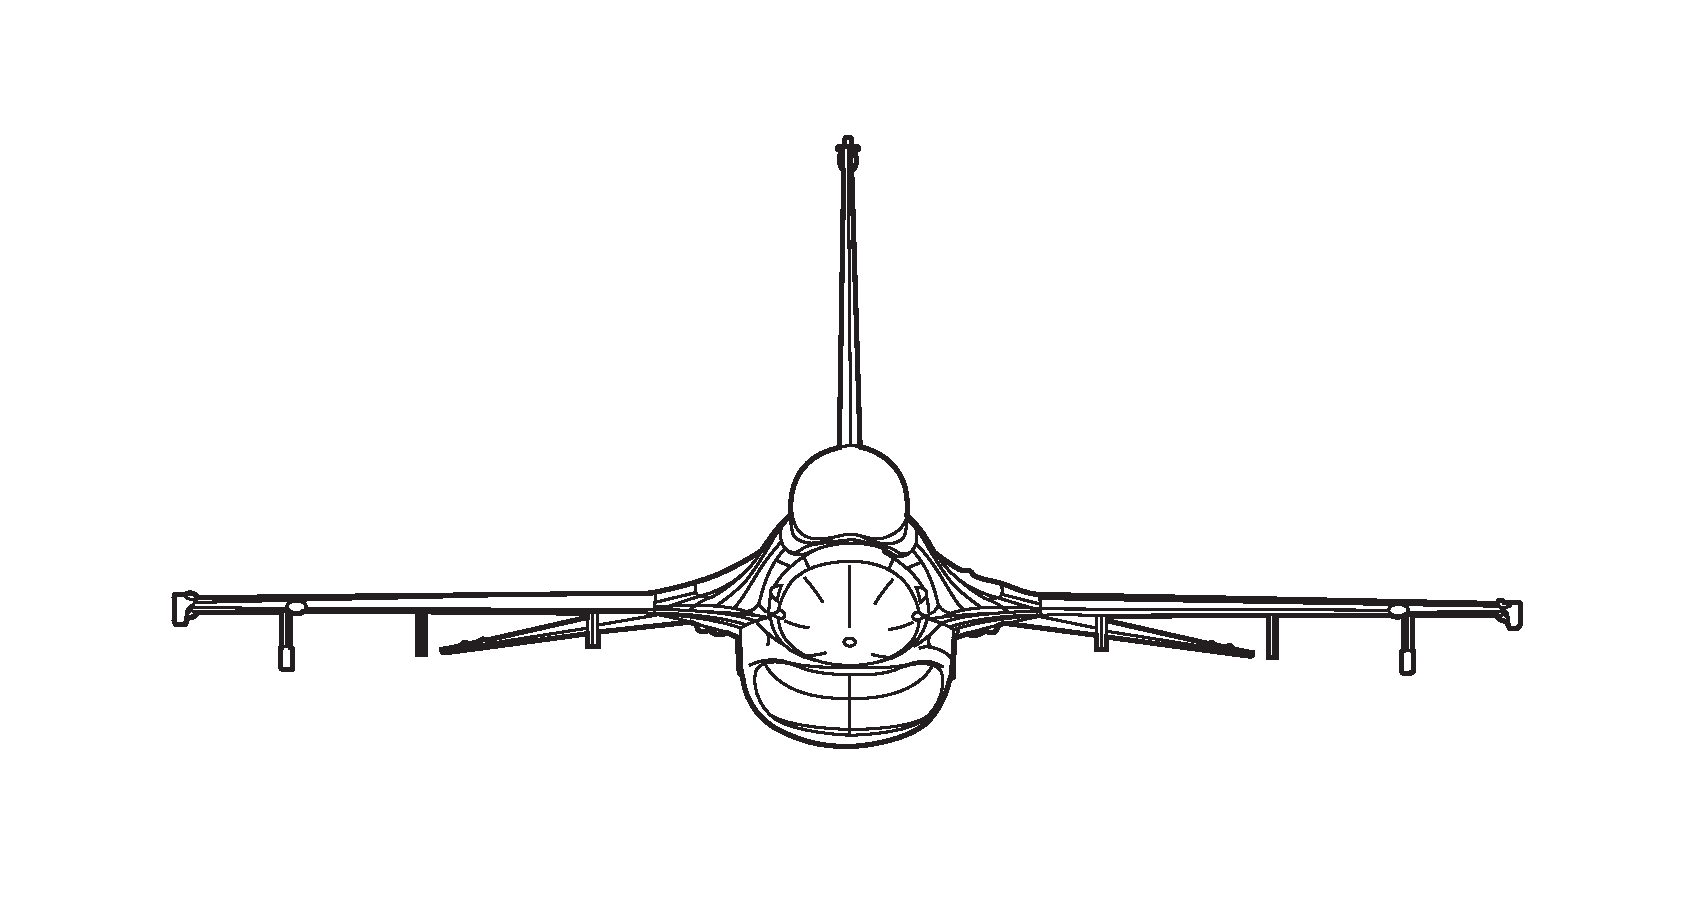
\includegraphics[%
				width=2\textwidth,%
			]{diagrams/aircraft/wireframe_front.pdf}%
		};
		% gold band for edition
		\node[
			anchor=south,
			xshift=-5mm,
			yshift=0mm,
			minimum width=\textwidth,
			font=\large,
			fill=techyellow,
		] (gold) at (current page text area.south) {%
			\fontspec[
				Path=./fonts/,
				Ligatures=TeX,
			]{Spartan MB-Medium Italic}%
			Gold Edition%
		};
		% authors
		\node[
			anchor=south east,
			xshift=-0mm,
			yshift=2em,
			font=\large,
		] (goldwolf) at (gold.north east) {
			\fontspec[
				Path=./fonts/,
				Ligatures=TeX,
			]{Spartan MB-Light Italic}%
			and Goldwolf%
		};
		\node[
			anchor=south east,
			xshift=-0mm,
			yshift=0em,
			font=\large,
		] (techneatium) at (goldwolf.north east) {
			\fontspec[
				Path=./fonts/,
				Ligatures=TeX,
			]{Spartan MB-Light Italic}
			By Techneatium%
		};
	\end{tikzpicture}

	% label for hyperrefs back to frontpage
	\label{frontpage}
	% make thumbfronts
	\thumbfront{Procedures \\ {\footnotesize Normal}}{0}{1}
	\cyclechpcolor%
	\thumbfront{Procedures \\ {\footnotesize Emergency}}{1}{2}
	\cyclechpcolor%
	\thumbfront{Aircraft \\ Systems}{2}{3}
	\cyclechpcolor%
	\thumbfront{Sensors \\ {\footnotesize A-A}}{3}{4}
	\cyclechpcolor%
	\thumbfront{Sensors \\ {\footnotesize A-G}}{4}{5}
	\cyclechpcolor%
	\thumbfront{Weapons \\ {\footnotesize A-G}}{5}{6}
	\cyclechpcolor%
	\thumbfront{Weapons \\ {\footnotesize A-A}}{6}{7}
	\cyclechpcolor%
	\thumbfront{Appendix}{7}{A}
	\thumbwide%

    \restoregeometry
	\clearpage

	\begin{tikzpicture}[overlay, remember picture]
		% logos
		\node[
			anchor=center,
			xshift=-\textwidth/4,
			yshift=-40mm,
		](logotc) at (current page text area.north) {%
			\IfFileExists{%
				figs/diagrams/logos/techschecks.pdf%
			}{%
				\includegraphics[%
					height=\textwidth/3,%
					page=1,%
				]{diagrams/logos/techschecks.pdf}%
			}{}%
		};
		\node[
			anchor=center,
			xshift=\textwidth/4,
			yshift=-40mm,
		](logogoldwolf) at (current page text area.north) {%
			\IfFileExists{%
				figs/diagrams/logos/goldwolf.pdf%
			}{%
				\includegraphics[%
					height=\textwidth/3,%
					page=1,%
				]{diagrams/logos/goldwolf.pdf}%
			}{}%
			
		};
		% thanks
		\node[
			anchor=south west,
			xshift=0mm,
			yshift=0mm,
			minimum width=\textwidth/1.5,
			text width=\textwidth/1.5,
			font=\normalsize,
			align=left,
		] (thanks) at (current page text area.south west) {%
			\fontspec[
				Path=./fonts/,
				Ligatures=TeX,
				LetterSpace=5.0,
			]{Spartan MB-Light Italic}
			Special thanks to \hfill\\
			\hfill Mythic \\
			\hfill TheMerryMarlin \\
			\hfill The UOAF Community
		};
		\node[
			anchor=south west,
			xshift=0mm,
			yshift=2em,
			minimum width=\textwidth/1.5,
			text width=\textwidth/1.5,
			font=\large,
			align=left,
		] (morkvitnir) at (thanks.north west) {%
			\fontspec[
				Path=./fonts/,
				Ligatures=TeX,
				LetterSpace=5.0,
			]{Spartan MB-Italic}
			Custom typefaces by \hfill\\
			\hfill Morkvitnir
		};
	\end{tikzpicture}
	\cleardoublepage
	\resetchpcolor


	\frontmatter
	\pagestyle{empty}
	\tableofcontents
\etocsettocstyle{}{}% removes "Contents" frome following tocs

\chapter*{BEFORE TAKEOFF READ THIS}
\thumbnar

\begin{tcolorbox}[
    enhanced, 
    colback=white, 
    colframe=color1, 
    colbacktitle=white, 
    coltitle=color1, 
    sharp corners, 
    attach boxed title to top center={yshift=2mm},
    boxed title style={
        sharp corners,
        drop shadow=color1!100
    }, 
    title=\LARGE\textbf{DISCLAIMER}
]
    \textbf{%
        This document represents a personal project
        and is intended for entertainment purposes only.
        Do not use for real life training purposes or scenarios.
    }
\end{tcolorbox}

\bigskip

\begin{multicols}{2}
    \cbstart {\Large\textbf{OBLIGATORY STEPS}}
    
    \medskip

    Procedural steps marked by solid bars long the page edge,
    as demonstrated here, 
    can not be skipped without impacting mission capability signficantly.

    \medskip 

    \textbf{Warning} -- this does \textbf{not} mean that all information which is not marked is therefore optional.
    \cbend 

    \vfill\null
    \columnbreak

    {\Large\textbf{NOTES AND WARNINGS}}

    \notebox{
        Additional information to be emphasized, usually related but not necessary information regarding a system or procedure.
    }

    \warningbox{
        Information which must be adhered to for proper system operation without malfunction or damage.
    }
\end{multicols}

\cleardoublepage
	
	% restart page counter, pagenumber styling
	\mainmatter
	% reactivate header and footer
	\pagestyle{body}

	\part{Procedures}
	\chapter{BASIC PROCEDURES}
\thumbtab{Procedures}{0}
\localtableofcontents
\cleardoublepage

\marginfigeometry

\section{START-UP}

\subsection{PRE-START}
\begin{checklistenumerate}
    \blueitem{\hyperref[fig:proc:prestart:flcscheck]{FLCS Check}}{
    \marginpar{
        \captionsetup{type=figure}
        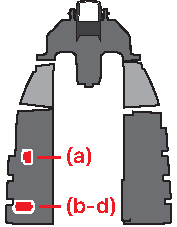
\includegraphics[width=\marginparwidth]{diagrams/cockpit/flcs_check.pdf}
        \caption{\textbf{FLCS Check}}
        \label{fig:proc:prestart:flcscheck}
    }
    \begin{subenumerate}
        \item \textbf{Main PWR Switch}\cbstart \dotfill \textbf{BATT}\cbend
        \begin{itemize}
            \item \textbf{FLCS RLY Light} --- \textbf{ON}
        \end{itemize}
        \item \textbf{FLCS PWR TEST} \dotfill \textbf{TEST (hold)}
        \item \textbf{Test Lights} \dotfill \textbf{Verify}
        \begin{itemize}
            \item \textbf{ACFT BATT TO FLCS} --- \textbf{ON}
            \item \textbf{FLCS PMG} --- \textbf{ON}
            \item \textbf{FLCS PWR} --- \textbf{ON}
            \item \textbf{FLCS RLY} --- \textbf{OFF}
        \end{itemize}
        \item \textbf{FLCS PWR TEST} \dotfill \textbf{Release}
    \end{subenumerate}}
    \blueitem{\hyperref[fig:proc:prestart:mainpower]{Main Power}}{
    \marginpar{
        \captionsetup{type=figure}
        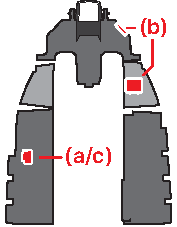
\includegraphics[width=\marginparwidth]{diagrams/cockpit/main_power.pdf}
        \caption{\textbf{Main Power}}
        \label{fig:proc:prestart:mainpower}
    }
    \begin{subenumerate}
        \item \textbf{Main PWR Switch}\cbstart \dotfill \textbf{MAIN}\cbend
        \item \textbf{Warning Lights} \dotfill \textbf{Check}
        \begin{itemize}
            \item \textbf{ELEC SYS} --- \textbf{ON}
            \item \textbf{HYD/OIL PRESS} --- \textbf{ON}
            \item \textbf{FLCS RLY} --- \textbf{ON}
            \item \textbf{SEC} --- \textbf{ON}
            \item \textbf{ENGINE} --- \textbf{ON}
        \end{itemize}
        \item \textbf{EPU Lights} \dotfill \textbf{Confirm OFF}
        \begin{itemize}
            \item \textbf{EPU GEN Light} --- \textbf{OFF}
            \item \textbf{EPU PMG Light} --- \textbf{OFF}
        \end{itemize}
    \end{subenumerate}}
\end{checklistenumerate}

\clearpage

\subsection{ENGINE START}
\begin{checklistenumerate}
    \blueitem{Engine Start}{\cbstart
    \marginpar{
        \captionsetup{type=figure}
        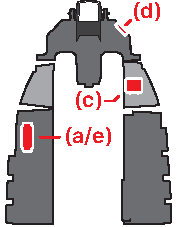
\includegraphics[width=\marginparwidth]{diagrams/cockpit/engine_start.pdf}
        \caption{\textbf{Engine Start}}
    }
    \begin{subenumerate}
        \item \textbf{JFS Switch} \dotfill \textbf{START 2}
        \item \textbf{Throttle} \dotfill \textbf{IDLE} \\
        \hfill (once 20\% RPM reached)
        \item \textbf{SEC Light} \dotfill \textbf{OFF} 
        \item \textbf{ENGINE Warning Light} \dotfill \textbf{OFF} \\
        \hfill (once 60\% RPM reached)
        \item \textbf{JFS Switch} \dotfill \textbf{Confirm OFF}
    \end{subenumerate}\cbend}
    \blueitem{ENG Instruments}{
    \marginpar{
        \captionsetup{type=figure}
        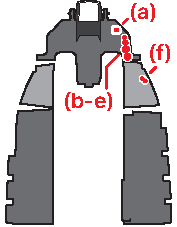
\includegraphics[width=\marginparwidth]{diagrams/cockpit/engine_instruments.pdf}
        \caption{\textbf{ENG Instruments}}
    }
    \begin{subenumerate}
        \item \textbf{FUEL FLOW} --- 700-1700 PPH
        \item \textbf{OIL Pressure} --- 15 PSI (minimum)
        \item \textbf{NOZ POS} --- greater than 95\%
        \item \textbf{RPM} --- 62-80\% 
        \item \textbf{FTIT} --- 650C or less
        \item \textbf{HYD PRES A \& B} --- 2850-3250 PSI
    \end{subenumerate}}
\end{checklistenumerate}

\notebox{
    \begin{itemize}
        \item \textbf{Can close Canopy prior to advancing Throttle to IDLE to reduce cockpit noise}
    \end{itemize}
}

\clearpage

\subsection{POST-START}
\begin{checklistenumerate}
    \blueitem{TEST Panel}{
    \marginpar{
        \captionsetup{type=figure}
        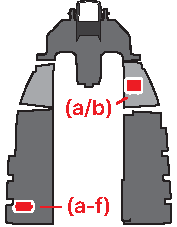
\includegraphics[width=\marginparwidth]{diagrams/cockpit/test_panel.pdf}
        \caption{\textbf{TEST Panel}}
    }
    \begin{subenumerate}
        \item \textbf{PROBE HEAT Switch} \dotfill \textbf{PROBE HEAT} \\
        \hfill verify PROBE HEAT Caution Light --- off
        \item \textbf{PROBE HEAT Switch} \dotfill \textbf{TEST} \\
        \hfill verify PROBE HEAT C. Light --- flashing
        \item \textbf{PROBE HEAT Switch} \dotfill \textbf{OFF}
        \item \textbf{FIRE \& OHEAT DETECT} \dotfill \textbf{TEST}
        \item \textbf{OXY QTY Test Switch} \dotfill \textbf{TEST}
        \item \textbf{MAL \& IND LTS Button} \dotfill \textbf{TEST}
    \end{subenumerate}}
    \blueitem{AVIONICS Panel}{\cbstart
    \marginpar{
        \captionsetup{type=figure}
        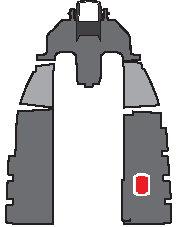
\includegraphics[width=\marginparwidth]{diagrams/cockpit/avionics_ins.pdf}
        \caption{\textbf{Avionics \& INS}}
    }
    \begin{subenumerate}
        \item \textbf{MMC Switch} \dotfill \textbf{MMC}
        \item \textbf{ST STA Switch} \dotfill \textbf{ST STA}
        \item \textbf{MFD Switch} \dotfill \textbf{MFD}
        \item \textbf{UFC Switch} \dotfill \textbf{UFD}
        \item \textbf{GPS Switch} \dotfill \textbf{GPS}
        \item \textbf{DL Switch} \dotfill \textbf{DL}
        \item \textbf{MIDS LVT Knob} \dotfill \textbf{ON}
    \end{subenumerate}}
    \blueitem{INS Alignment}{
    \begin{subenumerate}
        \item \textbf{EGI/INS} \dotfill \textbf{Desired ALIGN Mode} \\
        \begin{itemize}
            \item \textbf{NORM} --- full align, approx. 8 min
            \item \textbf{STOR HDG} --- quick align, approx. 90 sec
        \end{itemize}
    \end{subenumerate}}
    \blueitem{SNSR PWR Panel}{
    \marginpar{
        \captionsetup{type=figure}
        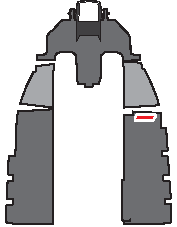
\includegraphics[width=\marginparwidth]{diagrams/cockpit/snsr_pwr.pdf}
        \caption{\textbf{SNSR PWR Panel}}
    }
    \begin{subenumerate}
        \item \textbf{LEFT HDPT Switch} \dotfill \textbf{As Required} \\
        \hfill (if HTS pod installed)
        \item \textbf{RIGHT HDPT Switch} \dotfill \textbf{As Required} \\
        \hfill (if targeting pod installed)
        \item \textbf{FCR Switch} \dotfill \textbf{FCR}
        \item \textbf{RDR ALT Switch} \dotfill \textbf{RDR ALT}
    \end{subenumerate}\cbend}
\end{checklistenumerate}

\clearpage

\begin{checklistenumerate}[resume]
    \blueitem{HUD Setup}{\cbstart
    \marginpar{
        \captionsetup{type=figure}
        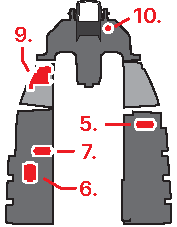
\includegraphics[width=\marginparwidth]{diagrams/cockpit/hud_sai.pdf}
        \caption{\textbf{HUD, C\&I, ECM, SPD BRK, WHEELS Down, SAI}}
    }
    \begin{subenumerate}
        \item \textbf{HUD Control Panel} \dotfill \textbf{As Desired}
        \item \textbf{HUD Brightness} \dotfill \textbf{As Desired} 
    \end{subenumerate}\cbend}
    \blueitem{C\&I Knob}{\textbf{UFC}}
    \blueitem{ECM Panel}{\cbstart\textbf{As Desired}\cbend}
    \blueitem{SPD BRK Check}{\textbf{Cycle} (back to closed)}
    \blueitem{WHEELS Down Lights}{Verify \textbf{Three Green}}
    \blueitem{\cbstart  Standby Attitude Indicator\cbend}{\textbf{Set}}
    \blueitem{Tests \& Checks}{\hyperref[subsec:testschecks]{\textbf{See \Cref{subsec:testschecks} Tests \& Checks}}}
% \end{checklistenumerate}

% \clearpage

% \begin{checklistenumerate}[resume]
    \blueitem{Avionics Setup}{
    \marginpar{
        \captionsetup{type=figure}
        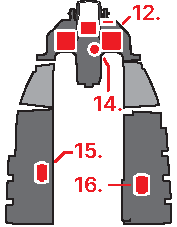
\includegraphics[width=\marginparwidth]{diagrams/cockpit/final_setup.pdf}
        \caption{\textbf{Final Setup}}
    }
    \cbstart\textbf{Program As Required}}
    \blueitem{Canopy}{\textbf{Close and Lock}}
    \blueitem{Altimeter}{\textbf{Set and Check}}
    \blueitem{Exterior Lights}{\textbf{As Desired}}
    \blueitem{INS Knob}{\textbf{NAV}\cbend}
    \blueitem{NWS}{\textbf{Engage}}
    \blueitem{Throttle}{\textbf{Advance} (Check brakes \& NWS)}
    \blueitem{Flight Instruments}{\textbf{Check}}
\end{checklistenumerate}

% \clearpage

\warningbox{
    \begin{itemize}
        \item \textbf{Aircraft Rearming can interrupt INS align}
        \begin{itemize}
            \item If interrupted recycle INS knob to off, then back to align
            \item Recommend rearming either before or after INS align
        \end{itemize}
    \end{itemize}
}

\clearpage

\subsection{TESTS \& CHECKS}
\label{subsec:testschecks}
\begin{checklistenumerate}
    \blueitem{ENG SEC Mode}{
    \marginpar{
        \captionsetup{type=figure}
        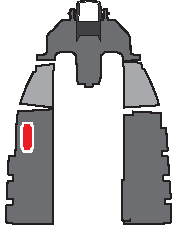
\includegraphics[width=\marginparwidth]{diagrams/cockpit/check_eng_sec.pdf}
        \caption{\textbf{ENG SEC Mode}}
    }
    \begin{subenumerate}
        \item \textbf{ENG CONT Switch} \dotfill \textbf{SEC}
        \begin{itemize}
            \item \textbf{SEC Caution Light} --- \textbf{ON}
            \item \textbf{RPM} --- Stabilized
            \item \textbf{Throttle} --- Snap to \textbf{MIL}, then to \textbf{IDLE} when RPM reaches 85\% 
            \item \textbf{NOZ POS} --- < 10\% within 30s after \textbf{SEC} selection
        \end{itemize}
        \item \textbf{ENG CONT Switch} \dotfill \textbf{PRI}
        \begin{itemize}
            \item \textbf{SEC Caution Light} --- \textbf{OFF}
            \item \textbf{NOZ POS} --- > 94\% 
        \end{itemize}
    \end{subenumerate}}
    \blueitem{FLCS BIT}{
    \marginpar{
        \captionsetup{type=figure}
        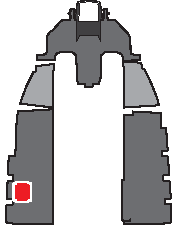
\includegraphics[width=\marginparwidth]{diagrams/cockpit/check_flcs_bit.pdf}
        \caption{\textbf{FLCS BIT}}
    }
    \begin{subenumerate}
        \item \textbf{FLCS BIT Switch} \dotfill \textbf{BIT}
        \begin{itemize}
            \item \textbf{FLCP RUN Light} --- Illuminates
        \end{itemize}
        \item \textbf{BIT Completion}
        \begin{itemize}
            \item \textbf{Duration} --- Approx. 45s
            \item \textbf{FLCP RUN Light} --- Extinguishes
            \item \textbf{BIT Switch} --- Returns to \textbf{OFF}
            \item \textbf{FAIL Light} --- Verify \textbf{OFF}
            \item \textbf{FLCS Warning Light} --- Verify \textbf{OFF}
        \end{itemize}
    \end{subenumerate}}
\end{checklistenumerate}

\clearpage

\begin{checklistenumerate}[resume]
    \blueitem{FUEL QTY Check}{
    \marginpar{
        \captionsetup{type=figure}
        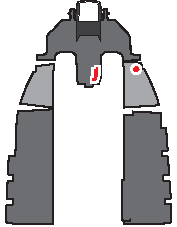
\includegraphics[width=\marginparwidth]{diagrams/cockpit/check_fuel_qty.pdf}
        \caption{\textbf{FUEL QTY Check}}
    }
    \begin{subenumerate}
        \item \textbf{FUEL QTY SEL Knob} \dotfill \textbf{TEST}
        \begin{itemize}
            \item \textbf{FR/AL Pointers} --- 2000 $\pm$ 100 lbs
            \item \textbf{Totalizer} --- 6000 $\pm$ 100 lbs
        \end{itemize}
        \item \textbf{FUEL QTY SEL Knob} \dotfill \textbf{NORM}
        \begin{itemize}
            \item \textbf{AL Pointer} --- 2675/2810 lbs
            \item \textbf{FR POINTER} --- 3100/3250 lbs
        \end{itemize}
        \item \textbf{FUEL QTY SEL Knob} \dotfill \textbf{RSVR}
        \begin{itemize}
            \item Each indicator approx. 460/480 lbs
        \end{itemize}
        \item \textbf{FUEL QTY SEL Knob} \dotfill \textbf{INT WING}
        \begin{itemize}
            \item Each indicator approx. 525/550 lbs
        \end{itemize}
        \item \textbf{FUEL QTY SEL Knob} \dotfill \textbf{EXT WING}
        \begin{itemize}
            \item Each indicator approx.\\
            \hfill 2300/2420 lbs  (if loaded)
        \end{itemize}
        \item \textbf{FUEL QTY SEL Knob} \dotfill \textbf{As Desired}
    \end{subenumerate}}
    \blueitem{DBU Check}{
    \marginpar{
        \captionsetup{type=figure}
        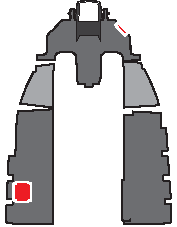
\includegraphics[width=\marginparwidth]{diagrams/cockpit/check_dbu.pdf}
        \caption{\textbf{DBU Check}}
    }
    \begin{subenumerate}
        \item \textbf{DIGITAL BACKUP Switch} \dotfill \textbf{BACKUP}
        \begin{itemize}
            \item \textbf{DBU ON Light} --- \textbf{Illuminates}
        \end{itemize}
        \item Operate Controls --- check for normal control surface response
        \item \textbf{DIGITAL BACKUP Switch} \dotfill \textbf{OFF}
    \end{subenumerate}}
    \blueitem{Trim Check}{
    \marginpar{
        \captionsetup{type=figure}
        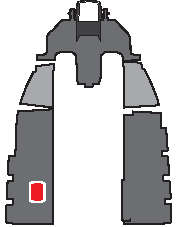
\includegraphics[width=\marginparwidth]{diagrams/cockpit/check_trim.pdf}
        \caption{\textbf{Trim Check}}
    }
    \begin{subenumerate}
        \item \textbf{TRIM/AP DISC Swtich} \dotfill \textbf{DISC}
        \item \textbf{Stick Trim} \dotfill Activate in Pitch \& Roll
        \begin{itemize}
            \item No control surface motion 
            \item No TRIM wheel or indicator motion
        \end{itemize} 
        \item \textbf{TRIM/AP DISC Swtich} \dotfill \textbf{NORM}
        \item \textbf{Stick Trim} \dotfill Check \& Center
        \begin{itemize}
            \item Control surface motion 
            \item TRIM wheel motion
        \end{itemize} 
        \item \textbf{Yaw Trim Knob} \dotfill \textbf{Center}
    \end{subenumerate}}
\end{checklistenumerate}

\clearpage

\begin{checklistenumerate}[resume]
    \blueitem{MPO Check}{
    \marginpar{
        \captionsetup{type=figure}
        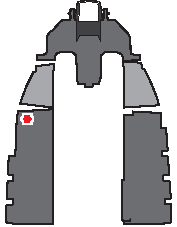
\includegraphics[width=\marginparwidth]{diagrams/cockpit/check_mpo.pdf}
        \caption{\textbf{MPO Check}}
    }
    \begin{subenumerate}
        \item \textbf{Stick} \dotfill \textbf{Full Forward \& Hold}
        \item \textbf{MPO Switch} \dotfill \textbf{OVRD \& Hold}
        \begin{itemize}
            \item Horizontal Tail trailing edges move farther down
        \end{itemize} 
        \item \textbf{Stick \& MPO} \dotfill Release
    \end{subenumerate}}
    \blueitem{EPU Check}{
    \marginpar{
        \captionsetup{type=figure}
        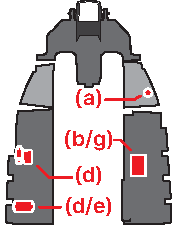
\includegraphics[width=\marginparwidth]{diagrams/cockpit/check_epu.pdf}
        \caption{\textbf{EPU Check}}
    }
    \begin{subenumerate}
        \item \textbf{EPU FUEL Qty} \dotfill \textbf{95-102 Percent}
        \item \textbf{OXYGEN} \dotfill \textbf{100\%}
        \item \textbf{Throttle} \dotfill 10\% above \textbf{IDLE}
        \item \textbf{EPU/GEN TEST Switch} \dotfill \textbf{EPU/GEN \& Hold}
        \begin{itemize}
            \item \textbf{EPU AIR Light} --- \textbf{ON}
            \item \textbf{EPU GEN/PMG Lights} --- \textbf{OFF}
            \item \textbf{FLCS PWR Lights} --- \textbf{ON}
            \item \textbf{EPU Run Light} --- \textbf{ON} minimum 5s
        \end{itemize} 
        \item \textbf{EPU/GEN TEST Switch} \dotfill \textbf{OFF}
        \item \textbf{Throttle} \dotfill \textbf{IDLE}
        \item \textbf{OXYGEN} \dotfill \textbf{NORMAL}
    \end{subenumerate}}
\end{checklistenumerate}

\marginfigrestore
\marginfigeometry

\section{TAKEOFF \& LANDING}

\subsection{PRE-TAKEOFF}
\begin{checklistenumerate}
    \blueitem[ALT FLAPS Switch]\dotfill\textbf{Verify Norm}
    \blueitem[Trim]\dotfill\textbf{Check}
    \blueitem[ENG CONT Switch]\dotfill\textbf{Verify PRI}
    \blueitem[Speedbrakes]\dotfill\textbf{Closed}
    \blueitem[Canopy]\dotfill\textbf{Verify Closed \& Locked}
    \blueitem[IFF]\dotfill\textbf{Set \& Check}
    \blueitem[FUEL QTY Select Knob]\dotfill\textbf{NORM}
    \blueitem[STORES CONFIG Switch]\dotfill\textbf{As Required}
    
    \begin{itemize}
        \item \textbf{CAT I} --- \textbf{A-A Loadouts} 
        \item \textbf{CAT III} --- \textbf{A-G / Wing tank Loadouts}
    \end{itemize}
    \blueitem[PROBE HEAT Switch]\dotfill\textbf{PROBE HEAT}
    \blueitem[Ejection Safety Lever]\cbstart\dotfill\textbf{Arm (down)}\cbend
    \blueitem[Flight Controls]\dotfill\textbf{Cycle}
    \blueitem[Oil Pressure]\dotfill\textbf{15-65 psi}
    \blueitem[TGP]\dotfill\textbf{STOW} (if installed)
    \blueitem[Warning \& Caution Lights]\dotfill\textbf{Verify Off}
\end{checklistenumerate}

\subsection{TAKEOFF}

\begin{checklistenumerate}
    \blueitem[Runup]\cbstart
    \begin{enumerate}
        \item \textbf{Brake} \dotfill \textbf{Hold}
        \item \textbf{Throttle} \dotfill \textbf{90\%}\cbend
    \end{enumerate}
    \blueitem[Runup Check]
    \begin{enumerate}
        \item \textbf{Parking Brake} \dotfill \textbf{Verify disengaged}
        \item \textbf{Engine Parameters} \dotfill \textbf{Nominal}
        \begin{itemize}
            \item \textbf{HYD/OIL PRES} --- \textbf{OFF}
            \item \textbf{Oil Pressure}
            \begin{itemize}
                \item \textbf{30-80 psi}
                \item \textbf{at least 15 psi higher than idle}
            \end{itemize}
            \item \textbf{FTIT} --- \textbf{less than 935deg}
            \item \textbf{HYD PRESS A \& B} --- \textbf{2850-3250psi}
        \end{itemize}
    \end{enumerate}
\end{checklistenumerate}

\clearpage

\begin{checklistenumerate}[resume]
    \blueitem[Takeoff Roll]\cbstart
    \marginpar{
        \captionsetup{type=table}
        \centering
        \caption{Takeoff Speeds}
        \label{tab:proc:takeoff:speed}
        \begin{tabular}{c c}
            \toprule 
            \textbf{Weight} & \textbf{TO Speed} \\
            \textbf{[lbs]} & \textbf{[kts]} \\
            \midrule 
            20000 & 128 \\
            \midrule 
            24000 & 142 \\
            \midrule 
            28000 & 156 \\
            \midrule 
            32000 & 168 \\
            \midrule 
            36000 & 178 \\
            \midrule 
            40000 & 188 \\
            \midrule 
            44000 & 198 \\
            \bottomrule
        \end{tabular}
    }
    \begin{enumerate}
        \item \textbf{Brake} \dotfill \textbf{Release}
        \item \textbf{Throttle} \dotfill \textbf{As Desired}\cbend
        \begin{itemize}
            \item \textbf{NOZ POS} --- \textbf{< 15\%} after 5 sec at \textbf{MIL/AB}
        \end{itemize}
    \end{enumerate}
    
    At 70 kts

    \begin{enumerate}[start=3]
        \item \textbf{NWS} \dotfill \textbf{Disengaged}
    \end{enumerate}
    \blueitem[Rotation]\cbstart
    At 10-15kts below takeoff speed, reference \cref{tab:proc:takeoff:speed}

    \begin{enumerate}
        \item \textbf{Attitude} \dotfill \textbf{8-12 deg nose high}
    \end{enumerate}

    Once positive rate has been achieved
    
    \begin{enumerate}[start=2]
        \item \textbf{Gear} \dotfill \textbf{UP}\cbend%
    \end{enumerate}%
    \marcautionbox{%
        \small\textbf{Exceeding 13 deg AOA can result in a tail strike!}%
    }%
\end{checklistenumerate}

\begin{figure}[htbp]
    \centering
    \begin{tikzpicture}[auto, node distance=10mm, x=1mm, y=1mm, very thick, line cap=round,
        >={Latex[round]}
        ]

        % coordinates
        \coordinate (startpoint) at (0,0);
        \coordinate (70kts) at (25,0);
        \coordinate (rotate) at (50,0);
        \coordinate (runwaystart) at (-5,-2.5);
        \coordinate (runwayend) at (70,-2.5);

        % runway
        \draw[thick, fill]
        ($(runwaystart)+(0,-0.25)$) -- ($(runwaystart)+(0,0.25)$) -- 
        ($(runwayend)+(0,0.25)$) -- ($(runwayend)+(0,-0.25)$) -- 
        cycle;

        % path
        \draw[very thick, ->]
        (startpoint) -- (70kts);
        \draw[very thick, ->]
        (70kts) -- (rotate);
        \draw[very thick, ->]
        (rotate) -- ++(5,0) arc (270:300:10) -- ++(30:10);

        % nodes
        \node[above, align=center] at (startpoint) {\small\textbf{Brakes} \\ \small\textbf{Runup}};
        \node[above, align=center] at (70kts) {\small\textbf{70kts} \\ \small\textbf{NWS Off}};
        \node[above, align=center] at (rotate) {\small\textbf{128-198kts} \\ \small\textbf{Rotate}};

    \end{tikzpicture}
    \caption{Takeoff Profile}
\end{figure}

\clearpage

\subsection{PRE-LANDING}

\begin{checklistenumerate}
    \blueitem[Fuel]\dotfill\textbf{Check}
    \blueitem[Landing Light]\dotfill\textbf{ON}
    \blueitem[Altimeter]\dotfill\textbf{Set \& Check}
    \blueitem[Attitude References]\dotfill\textbf{Check}
    \blueitem[Anti-Ice]\dotfill\textbf{As Required}
    \blueitem[TGP]\dotfill\textbf{STOW} (if installed)
\end{checklistenumerate}

\subsection{LANDING}

\begin{checklistenumerate}
    \blueitem[Approach] Align aircraft with runway
    \marginpar{
        \captionsetup{type=figure}
        \centering
        \begin{tikzpicture}[figstyle]

            % coordinates
            \coordinate (approach) at (5,-15);
            \coordinate (break) at (5,20);
            \coordinate (downwind) at (-15,20);
            \coordinate (base) at (-15,-15);
            \coordinate (final) at (-7.5,-22.5);
            \coordinate (shortfinal) at (0,-15);
            \coordinate (touchdown) at (0,0);
            \coordinate (rollout) at (0,20);

            % runway
            \draw[thick]
            ($(touchdown)+(-2,-5)$) -- ($(touchdown)+(2,-5)$) -- 
            ($(touchdown)+(2,25)$) -- ($(touchdown)+(-2,25)$) -- 
            cycle;
            \draw[thick]
            ($(touchdown)+(-1.33,-1)$) -- ($(touchdown)+(-1.33,1)$)
            ($(touchdown)+(-0.66,-1)$) -- ($(touchdown)+(-0.66,1)$)
            ($(touchdown)+(0.66,-1)$) -- ($(touchdown)+(0.66,1)$)
            ($(touchdown)+(1.33,-1)$) -- ($(touchdown)+(1.33,1)$);

            % pattern
            \draw[ultra thick, ->] 
            (approach) -- (break);
            \draw[ultra thick] 
            (break) arc (0:180:10);
            \draw[ultra thick, >->] 
            (downwind) -- (base);
            \draw[ultra thick] 
            (base) arc (180:270:7.5);
            \draw[ultra thick] 
            (final) arc (270:360:7.5);
            \draw[ultra thick, >-] 
            (shortfinal) -- (touchdown);
            \draw[ultra thick, ->] 
            (touchdown) -- (rollout);

            % nodes
            \node[right] at (approach) {\textbf{1.}};
            \node[right] at (break) {\textbf{2.}};
            \node[left] at (downwind) {\textbf{3.}};
            \node[left] at (base) {\textbf{4.}};
            \node[below] at (final) {\textbf{5.}};
            \node[left] at (shortfinal) {\textbf{6.}};
            \node[left=2mm] at (touchdown) {\textbf{7.}};
            \node[left=2mm] at (rollout) {\textbf{8.}};

        \end{tikzpicture}
        \caption{Overhead pattern}
        \label{fig:proc_basic:landing:overhead}
    }

    \marnotebox{
        \small\textbf{\Cref{fig:proc_basic:landing:overhead,fig:proc_basic:landing:overhead2} are illustrated with extended approach and downwind sections for clarity}
    }

    \begin{itemize}
        \item \textbf{Altitude} --- \textbf{1500 ft AGL}
        \item \textbf{Airspeed} --- \textbf{300 kts CAS}
    \end{itemize}
    \blueitem[Overhead Break] Break left/right over desired touchdown point, \textbf{\underline{maintain level turn}}

    \begin{itemize}
        \item \textbf{Speedbrakes} --- \textbf{As Required}
        \item \textbf{Throttle} --- \textbf{As Required}
        \item \textbf{Bank} --- \textbf{70 deg}
        \item \textbf{Break} --- \textbf{1\% of airspeed in G}
    \end{itemize}
    \blueitem[Downwind Leg] Roll out on opposite heading of runway, max 13 deg AoA

    \begin{itemize}
        \item \textbf{Altitude} --- \textbf{1500 ft AGL}
        \item \textbf{Airspeed} --- \textbf{200-220 kts CAS}
        \item \textbf{Gear} --- \textbf{Down}
    \end{itemize}
    \blueitem[Base Turn] Initiate abeam of desired touchdown point (wingtip at end of runway)

    \begin{itemize}
        \item \textbf{Attitude} --- \textbf{8-10 deg nose low}
        \item \textbf{AoA} --- \textbf{< 13 deg}
    \end{itemize}
    \blueitem[Final Turn] Use throttle to maintain AoA, stick to maintain attitude, goal is to roll wings-level at

    \begin{itemize}
        \item \textbf{1 mile} from desired touchdown point
        \item \textbf{Altitude} --- \textbf{300 ft AGL}
        % \item \textbf{AoA} --- \textbf{max 13 deg}
        \item \textbf{Flightpath} --- align  with \textbf{2.5 deg HUD marker} and runway threshold
    \end{itemize}
\end{checklistenumerate}

\clearpage

\begin{checklistenumerate}[resume]
    \blueitem[Short Final] Once over runway
    
    \marginpar{
        \captionsetup{type=figure}
        \centering
        \begin{tikzpicture}[figstyle]

            % coordinates
            \coordinate (approach) at (5,-15);
            \coordinate (break) at (5,20);
            \coordinate (downwind) at (-15,20);
            \coordinate (base) at (-15,-15);
            \coordinate (final) at (-7.5,-22.5);
            \coordinate (shortfinal) at (0,-15);
            \coordinate (touchdown) at (0,0);
            \coordinate (rollout) at (0,20);

            % runway
            \draw[thick]
            ($(touchdown)+(-2,-5)$) -- ($(touchdown)+(2,-5)$) -- 
            ($(touchdown)+(2,25)$) -- ($(touchdown)+(-2,25)$) -- 
            cycle;
            \draw[thick]
            ($(touchdown)+(-1.33,-1)$) -- ($(touchdown)+(-1.33,1)$)
            ($(touchdown)+(-0.66,-1)$) -- ($(touchdown)+(-0.66,1)$)
            ($(touchdown)+(0.66,-1)$) -- ($(touchdown)+(0.66,1)$)
            ($(touchdown)+(1.33,-1)$) -- ($(touchdown)+(1.33,1)$);

            % pattern
            \draw[ultra thick, ->] 
            (approach) -- (break);
            \draw[ultra thick] 
            (break) arc (0:180:10);
            \draw[ultra thick, >->] 
            (downwind) -- (base);
            \draw[ultra thick] 
            (base) arc (180:270:7.5);
            \draw[ultra thick] 
            (final) arc (270:360:7.5);
            \draw[ultra thick, >-] 
            (shortfinal) -- (touchdown);
            \draw[ultra thick, ->] 
            (touchdown) -- (rollout);

            % nodes
            \node[right] at (approach) {\textbf{1.}};
            \node[right] at (break) {\textbf{2.}};
            \node[left] at (downwind) {\textbf{3.}};
            \node[left] at (base) {\textbf{4.}};
            \node[below] at (final) {\textbf{5.}};
            \node[left] at (shortfinal) {\textbf{6.}};
            \node[left=2mm] at (touchdown) {\textbf{7.}};
            \node[left=2mm] at (rollout) {\textbf{8.}};

        \end{tikzpicture}
        \caption{Overhead pattern (duplicated)}
        \label{fig:proc_basic:landing:overhead2}
    }

    \begin{itemize}
        \item \textbf{Flightpath} --- shift \textbf{300-500 ft} down runway
        \item \textbf{Flare} --- gently pull back on stick
        \item \textbf{Throttle} --- \textbf{Idle}
        \item \textbf{AoA} --- \textbf{< 13 deg}
    \end{itemize}
    \blueitem[Touchdown]
    \blueitem[Landing Roll] Maintain nose-high position for aerobraking until 100 kts
    \begin{itemize}
        \item \textbf{AoA} --- \textbf{< 13 deg}
        \item \textbf{Speedbrakes} --- \textbf{Open}
        \item \textbf{Brakes} --- \textbf{As Required}
    \end{itemize}
    \blueitem[Taxi]
    \begin{itemize}
        \item \textbf{NWS} --- \textbf{Engaged}
    \end{itemize}
\end{checklistenumerate}

\clearpage

\subsection{POST-LANDING}
\begin{checklistenumerate}
    \blueitem[PROBE HEAT Switch]\dotfill\textbf{OFF}
    \blueitem[ECM Power]\dotfill\textbf{OFF}
    \blueitem[Speedbrakes]\dotfill\textbf{Close}
    \blueitem[Ejection Safety Lever]\dotfill\textbf{Safe (up)}
    \blueitem[IFF Master Knob]\dotfill\textbf{STBY}
    \blueitem[Landing/Taxi Light]\dotfill\textbf{As Desired}
    \blueitem[Armament Switches]\dotfill\textbf{Safe}
    \blueitem[Avionics]\dotfill\textbf{Off}
    \begin{itemize}
        \item \textbf{HUD Thumbwheels} --- \textbf{Off}
        \item \textbf{SNSR PWR Switches} --- \textbf{Off}
        \item \textbf{AVIONICS PWR Switches} --- \textbf{Off}
    \end{itemize}
    \blueitem[Engine Shutdown]
    \begin{enumerate}
        \item \textbf{Throttle} \dotfill \textbf{Off}
        \item \textbf{Lights} \dotfill \textbf{Check}
        \begin{itemize}
            \item \textbf{JFS Light} --- \textbf{Off}
            \item \textbf{EPU GEN Light} --- \textbf{Off}
            \item \textbf{EPU PMG Light} --- \textbf{Off}
        \end{itemize}
        \item \textbf{Main PWR Switch} \dotfill \textbf{OFF}
    \end{enumerate}
    \blueitem[Oxygen Regulator]\dotfill\textbf{Off}
    \blueitem[Canopy]\dotfill\textbf{Open}
\end{checklistenumerate}

\marginfigrestore
\marginfigeometry

\section{IN-FLIGHT}

\subsection{AIR-TO-AIR REFUELING}

\begin{checklistenumerate}
    \blueitem{Safe Aircraft}{
    \marginpar{
        \captionsetup{type=figure}
        \centering
        \begin{tikzpicture}[auto, node distance=10mm, x=1mm, y=1mm, very thick, line cap=round,
            >={Latex[round]}
            ]
            
            \node[] (fig) at (0,0) {
                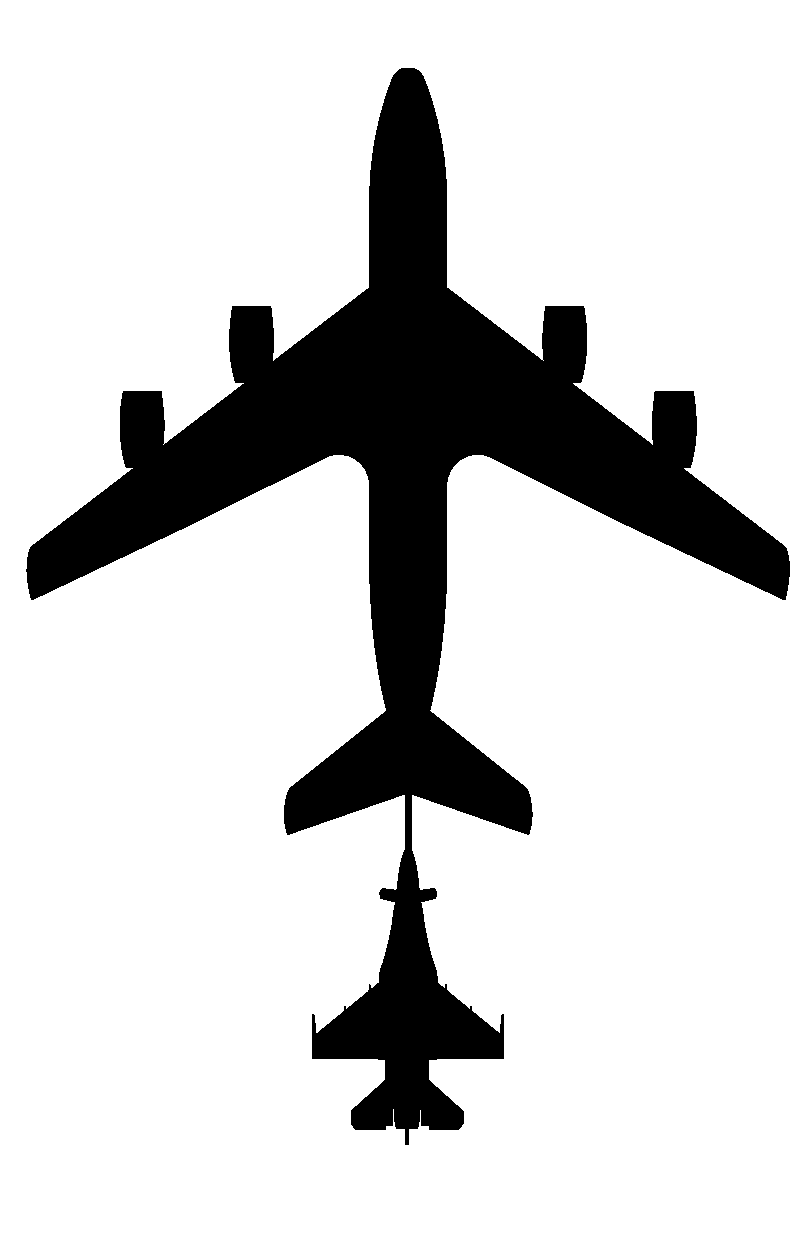
\includegraphics[
                    width=0.5\marginparwidth,
                    angle=270,
                ]{diagrams/aircraft/silhouette_tanker_f16_top.pdf}
            };
    
            % Annotations
            \node[
                draw, 
                ellipse, 
                dashed, 
                font=\footnotesize, 
                align=center,
                minimum width=25mm,
                minimum height=15mm,
                yshift=8mm,
                xshift=8mm,
            ] (obs) at (fig.north west) {Observation \\ area};
            \node[
                dashed, 
                font=\footnotesize, 
                align=center,
                anchor=east,
                xshift=3mm,
            ] (fuel) at (fig.west) {Refueling \\ area};
            \node[
                draw, 
                ellipse, 
                dashed, 
                font=\footnotesize, 
                align=center,
                minimum width=25mm,
                minimum height=15mm,
                yshift=-8mm,
                xshift=8mm,
            ] (reform) at (fig.south west) {Reform \\ area};
        \end{tikzpicture}
        \caption{Refueling areas}
        \label{fig:proc_basic:aarefueling:areas}
    }
    \begin{subenumerate}
        \item \textbf{Master Arm} \dotfill \textbf{OFF}
        \item \textbf{Laser Arm} \dotfill \textbf{OFF}
        \item \textbf{RF Switch} \dotfill \textbf{SILENT}
    \end{subenumerate}}
    \blueitem{Configure for Refueling}{
    \begin{subenumerate}
        \item \textbf{AIR REFUEL Switch}\cbstart \dotfill \textbf{Open}
        \item \textbf{AR Status Light} \dotfill \textbf{Verify RDY}\cbend
        \item \textbf{HOT MIC/CIPHER Switch} \dotfill \textbf{HOT MIC}
        \item \textbf{Exterior Lights} \dotfill \textbf{As required}
        \item \textbf{DED BINGO Page} \dotfill \textbf{Monitor}
    \end{subenumerate}
    
    If DED mirroring to HUD is desired 
    
    \begin{subenumerate}[start=6]
        \item \textbf{DED Data/PFL Switch} \dotfill \textbf{DED Data} 
    \end{subenumerate}}
    \blueitem{Refuel\cbstart}{
    \marginpar{
        \captionsetup{type=figure}
        \centering
        \begin{tikzpicture}[auto, node distance=10mm, x=1mm, y=1mm, very thick, line cap=round,
            >={Latex[round]}
            ]
            
            \node[] (figl) at (-5,0) {
                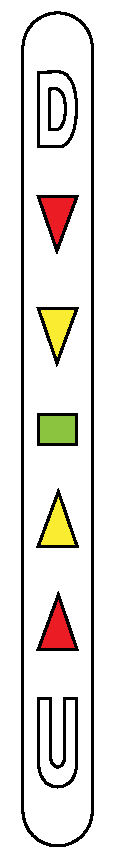
\includegraphics[
                    height=\marginparwidth,
                ]{diagrams/aircraft/tanker_lights_vertical.pdf}
            };

            \node[] (figr) at (5,0) {
                
\includegraphics[
                    height=\marginparwidth,
                ]{diagrams/aircraft/tanker_lights_longitudinal.pdf}
            };

            % Annotations
            \node[lannot, text width=8mm, font=\footnotesize] (mode) at ($(figl.west)+(-1mm,15mm)$) {Down};
            \draw[annotptr] (mode.east) -- ++(3mm, 0mm);

            \node[lannot, text width=8mm, font=\footnotesize] (mode) at ($(figl.west)+(-1mm,-15mm)$) {Up};
            \draw[annotptr] (mode.east) -- ++(3mm, 0mm);
            
            \node[rannot, text width=8mm, font=\footnotesize] (mode) at ($(figr.east)+(1mm,15mm)$) {Fwd};
            \draw[annotptr] (mode.west) -- ++(-3mm, 0mm);
            
            \node[rannot, text width=8mm, font=\footnotesize] (mode) at ($(figr.east)+(1mm,-15mm)$) {Aft};
            \draw[annotptr] (mode.west) -- ++(-3mm, 0mm);
        \end{tikzpicture}
        \caption{Tanker director lights, can be considered as commands to pilot}
        \label{fig:proc_basic:aarefueling:lights}
    }
    \begin{subitemize}
        \item Fly into refueling area, reference \cref{fig:proc_basic:aarefueling:areas}, allow boom operator to fly boom into refueling port
        \item \textbf{AR/NWS Light} illuminates to indicate contact
        \item Reference director lights to maintain position within boom limits, reference \cref{fig:proc_basic:aarefueling:lights}
        \item Monitor refueling progress on DED/HUD
    \end{subitemize}}
    \blueitem{Post-Refueling}{
    \begin{subenumerate}
        \item \textbf{A/R DISC Button} \dotfill \textbf{Press}
        \item \textbf{AIR REFUEL Switch} \dotfill \textbf{Close}\cbend
        \item \textbf{HOT MIC/CIPHER Switch} \dotfill \textbf{OFF}
        \item \textbf{FUEL QTY} \dotfill \textbf{Check}
        \item \textbf{AR Status Light} \dotfill \textbf{Verify Off}
        \item \textbf{Exterior Lights} \dotfill \textbf{As required}
    \end{subenumerate}}
    \blueitem{Rearm Aircraft}{
    \begin{subenumerate}
        \item \textbf{RF Switch} \dotfill \textbf{As Required}
        \item \textbf{Laser Arm} \dotfill \textbf{As Required}
        \item \textbf{Master Arm} \dotfill \textbf{As Required}
    \end{subenumerate}}
\end{checklistenumerate}

\marginfigrestore

\cleardoublepage
	\cyclechpcolor
	\chapter[EMERGENCY PROCEDURES --- WIP]{EMERGENCY PROCEDURES}
\thumbtab{Em Proc}{1}
\localtableofcontents
\thispagestyle{plain}
\cleardoublepage
	\part{Systems}
	\cyclechpcolor
	\chapter{AIRCRAFT SYSTEMS --- WIP}
\thumbtab{A/C Systems}{1}
\localtableofcontents
\thispagestyle{plain}
\cleardoublepage

% \section{FLIGHT CONTROL SYSTEMS}

% \clearpage

% \section{NAVIGATION SYSTEMS}

% \clearpage

% \section{COMMUNICATION SYSTEMS}

% \clearpage

% \section{DEFENSIVE SYSTEMS}

% \clearpage

% \cleardoublepage
	\cyclechpcolor
	\chapter{A-A SENSORS}
\thumbtab{A-A SENSORS}{2}
\localtableofcontents
\cleardoublepage

\section{APG-68 FCR}

\subsection{OVERVIEW}
\begin{tcoloritemize}
    \blueitem{A-A Modes}{
    \begin{subitemize}
        \item \textbf{CRM} --- \textbf{C}ombined \textbf{R}adar \textbf{M}ode, \break see \Cref{subsec:crm}
        \begin{itemize}
            \item \textbf{RWS} --- \textbf{R}ange \textbf{W}hile \textbf{S}earch, \break see \Cref{subsec:rws}
            \item \textbf{TWS} --- \textbf{T}rack \textbf{W}hile \textbf{S}can, \break see \Cref{subsec:tws}
        \end{itemize}
        \item \textbf{ACM} --- \textbf{A}ir \textbf{C}ombat \textbf{M}ode, see \Cref{subsec:acm}
        \item \textbf{STT} --- \textbf{S}ingle \textbf{T}arget \textbf{T}rack, see \Cref{subsec:stt}
    \end{subitemize}}
    \blueitem{A-G Modes}{\textbf{Work In Progress}
    \begin{subitemize}
        \item \textbf{GM} --- \textbf{G}round \textbf{M}ap
        \item \textbf{GMT} --- \textbf{G}round \textbf{M}oving \textbf{T}arget
    \end{subitemize}}
\end{tcoloritemize}

\begin{figure}[htbp]
    \centering
    \begin{tikzpicture}[auto, node distance=10mm,x=1mm, y=1mm, very thick,
        >={Latex[round]}
        ]
        
        % \node[<options>](<coordinate name>)at(<coordinate>){<text>};
        \node[
            hyperref node=subsec:stt,
            rectangle, 
            rounded corners,
            minimum width=90mm,
            minimum height=7.5mm,
            draw,
        ](stt)at(0,0){\blue{STT}--- \Cref{subsec:stt}};
        \node[
            hyperref node=subsec:crm,
            rectangle,
            rounded corners,
            minimum width=25mm,
            minimum height=7.5mm,
            draw,
        ](crm)at(0,30){\begin{tabular}{c}\blue{CRM}\\ \Cref{subsec:crm}\end{tabular}};
        \node[
            hyperref node=subsec:rws,
            rectangle,
            rounded corners,
            minimum width=25mm,
            minimum height=7.5mm,
            draw,
        ](rws)at(0,15){\begin{tabular}{c}\blue{RWS}\\ \Cref{subsec:rws}\end{tabular}};
        \node[
            hyperref node=subsec:tws,
            rectangle,
            rounded corners,
            minimum width=25mm,
            minimum height=7.5mm,
            draw,
        ](tws)at(32.5,15){\begin{tabular}{c}\blue{TWS}\\ \Cref{subsec:tws}\end{tabular}};
        \node[
            hyperref node=subsec:acm,
            rectangle,
            rounded corners,
            minimum width=25mm,
            minimum height=7.5mm,
            draw,
        ](acm)at(0,-30){\begin{tabular}{c}\blue{ACM}\\ \Cref{subsec:acm}\end{tabular}};
        \node[
            rectangle,
            rounded corners,
            minimum width=25mm,
            minimum height=7.5mm,
            draw,
        ](bore)at(0,-15){\textbf{BORE}};
        \node[
            rectangle,
            rounded corners,
            minimum width=25mm,
            minimum height=7.5mm,
            draw,
        ](hud)at(32.5,-30){\textbf{HUD}};
        \node[
            rectangle,
            rounded corners,
            minimum width=25mm,
            minimum height=7.5mm,
            draw,
        ](vert)at(0,-45){\textbf{Vertical}};

        % Lines
        \draw [->]
            (crm) -- (rws);
        \draw [->, rounded corners]
            (crm) -| (tws);
        \draw [->]
            let
                \p1=(rws.south),
                \p2=(stt.north),
            in
                (\p1) -- (\x1,\y2);
        \draw [->]
            let
                \p1=(tws.south),
                \p2=(stt.north),
            in
                (\p1) -- (\x1,\y2);
        \draw [->]
            (acm) -- (bore);
        \draw [->]
            (acm) -- (hud);
        \draw [->]
            (acm) -- (vert);
        \draw [->]
            let
                \p1=(bore.north),
                \p2=(stt.south),
            in
                (\p1) -- (\x1,\y2);
        \draw [->]
            let
                \p1=(hud.north),
                \p2=(stt.south),
            in
                (\p1) -- (\x1,\y2);
        \draw [->, rounded corners]
            let
                \p1=(vert.west),
                \p2=(stt.south),
            in
                (\p1) -- (\x1-22.5mm,\y1) -- (\x1-22.5mm,\y2);
                
    \end{tikzpicture}
    \caption{\textbf{A-A Radar Modes Overview}}
\end{figure}

\subsection{CRM}
\label{subsec:crm}

\begin{tcoloritemize}
    \blueitem{CRM}{
        \textbf{C}ombined \textbf{R}adar \textbf{M}ode --- Combines A-A search submodes:

        \begin{subitemize}
            \item \textbf{RWS} --- \textbf{R}ange \textbf{W}hile \textbf{S}earch,
            see \Cref{subsec:rws}
            \item \textbf{TWS} --- \textbf{T}rack \textbf{W}hile \textbf{S}can,
            see \Cref{subsec:tws}
        \end{subitemize}

        Selected by default on FCR start-up
    }
    \blueitem{Change CRM \break Submode}{
    \begin{subitemize}
        \item \textbf{OSB 2} \dotfill \textbf{Press}
        \item Or \textbf{TMS} \dotfill \textbf{Right Long}
    \end{subitemize}}
\end{tcoloritemize}

\begin{figure}[htbp]
    \centering
    \begin{tikzpicture}[auto, node distance=10mm,x=1mm, y=1mm, very thick,
        >={Latex[round]}
        ]
        
        \path[
            fill=color2!20,
            rounded corners,
        ] (-50,90) -- (50,90) -- (50,45) -- (-50,45) -- cycle;
        \node[
            anchor=north west,
        ](mark)at(-50,90){\scriptsize \blue{Supports AIM-120 Launch}};
        \path[
            fill=color2!60,
            rounded corners,
        ] (-47.5,85) -- (0,85) -- (0,90) -- (50,90) -- (50,75) -- (-47.5,75) -- cycle;
        \node[
            anchor=north east,
        ](mark)at(50,90){\scriptsize \textbf{\color{white}RWR Launch Warning}};
        % \node[<options>](<coordinate name>)at(<coordinate>){<text>};
        \node[
            hyperref node=subsec:rws,
            rectangle,
            rounded corners,
            minimum width=15mm,
            minimum height=15mm,
            draw,
        ](rws)at(0,0){\blue{RWS}};
        \node[
            rectangle,
            rounded corners,
            minimum width=25mm,
            minimum height=7.5mm,
            draw,
            fill=white,
        ](sam)at(0,50){\textbf{SAM}};
        \node[
            rectangle,
            rounded corners,
            minimum width=25mm,
            minimum height=7.5mm,
            draw,
            fill=white,
        ](dtt)at(-32.5,65){\textbf{DTT}};
        \node[
            hyperref node=subsec:tws,
            rectangle,
            rounded corners,
            minimum width=15mm,
            minimum height=15mm,
            draw,
        ](tws)at(32.5,0){\blue{TWS}};
        \node[
            rectangle,
            rounded corners,
            minimum width=25mm,
            minimum height=7.5mm,
            draw,
            fill=white,
        ](systgt)at(32.5,20){\textbf{System Tgt}};
        \node[
            rectangle,
            rounded corners,
            minimum width=25mm,
            minimum height=7.5mm,
            draw,
            fill=white,
        ](cursortgt)at(32.5,35){\textbf{Cursor Tgt}};
        \node[
            rectangle,
            rounded corners,
            minimum width=25mm,
            minimum height=7.5mm,
            draw,
            fill=white,
        ](bug)at(32.5,50){\textbf{Bugged}};
        \node[
            hyperref node=subsec:stt,
            rectangle, 
            rounded corners,
            minimum width=90mm,
            minimum height=7.5mm,
            draw, 
            fill=white,
        ](stt)at(0,80){\blue{STT}};
        
        % Lines
        \draw [->]
            (rws) -- node[pos=0.5, left]{\scriptsize\textbf{TMS FWD}} (sam);
        \draw [<->]
            (rws) -- node[pos=0.5, above]{\scriptsize\textbf{TMS RIGHT}}node[pos=0.5, below]{\scriptsize\textbf{(long)}} (tws);
        \draw [->, rounded corners]
            (sam) -| node[pos=0.25, above]{\scriptsize\textbf{TMS FWD}}node[pos=0.25, below]{\scriptsize\textbf{(2nd Tgt)}} (dtt);
        \draw [->]
            (tws) -- node[pos=0.5, left]{\scriptsize\textbf{TMS FWD}} (systgt);
        \draw [->]
            (systgt) -- node[pos=0.5, left]{\scriptsize\textbf{Cursor Over}} (cursortgt);
        \draw [->]
            (cursortgt) -- node[pos=0.5, left]{\scriptsize\textbf{TMS FWD}} (bug);
        \draw [->]
            let
                \p1=(dtt.north),
                \p2=(stt.south)
            in
                (\p1) -- node[pos=0.5, left]{\scriptsize\textbf{TMS FWD}} (\x1,\y2);
        \draw [->]
            let
                \p1=(sam.north),
                \p2=(stt.south)
            in
                (\p1) -- node[pos=0.5, left]{\scriptsize\textbf{TMS FWD}}node[pos=0.5, right]{\scriptsize\textbf{(1st Tgt)}} (\x1,\y2);
        \draw [->]
            let
                \p1=(bug.north),
                \p2=(stt.south)
            in
                (\p1) -- node[pos=0.5, left]{\scriptsize\textbf{TMS FWD}} (\x1,\y2);
    \end{tikzpicture}
    \caption{\textbf{CRM Radar Modes Overview}}
    \label{fig:crmoverview}
\end{figure}

\clearpage

\subsubsection{A-A SEARCH SCAN PATTERN}

\begin{tcoloritemize}
    \blueitem{Radar Gimbal Limits}{
    APG-68 is mechanically scanned on 2 axis gimbal

    \begin{subitemize}
        \item \textbf{Azimuth} --- \pm60 deg (120 deg coverage)
        \item \textbf{Vertical} --- \pm60 deg (120 deg coverage)
    \end{subitemize}}
    \blueitem{Azimuth Scan Pattern}{
    Horizontal scan volume controlled by selecting limits of gimbal azimuth
    \begin{subitemize}
        \item \textbf{Azimuth search patterns}
        \begin{itemize}
            \item \textbf{A6} --- \pm60 deg
            \item \textbf{A3} --- \pm30 deg (centered on cursor)
            \item \textbf{A1} --- \pm10 deg (centered on cursor)
        \end{itemize}
        \item \textbf{Cycled via}
        \begin{itemize}
            \item \textbf{OSB 18} cycles available azimuth patterns
            \item Walking cursor off side of FCR display in RWS cycles A6/A3
        \end{itemize}
        \item \textbf{TWS \& DTT modes use a special \pm25 deg, \\ 
        3 bar scan pattern}
        \begin{itemize}
            \item \textbf{A2} --- \pm25 deg (centered on cursor / target)
        \end{itemize}
    \end{subitemize}
    Reference \cref{fig:sensors_aa:apg68:crm:azscan} for graphical representation
    }
    \blueitem{Bar Scan Pattern}{
    Elevation scan volume controlled by selecting number of ``bars'' (horizontal sweeps)
    \begin{subitemize}
        \item \textbf{B4} / \textbf{B2} / \textbf{B1} --- cycled via \textbf{OSB 17}
        \item \textbf{B3} --- selected by TWS \& DTT modes
    \end{subitemize}
    Reference \cref{fig:sensors_aa:apg68:crm:barscan} for graphical representation
    }
\end{tcoloritemize}

\begin{figure}[htbp]
    \centering
    \begin{tikzpicture}[auto, node distance=10mm, x=1mm, y=1mm, very thick, line cap=round,
        >={Latex[round]}
        ]

        \node[
            anchor=east
        ] (mfd) at (0,0) {
            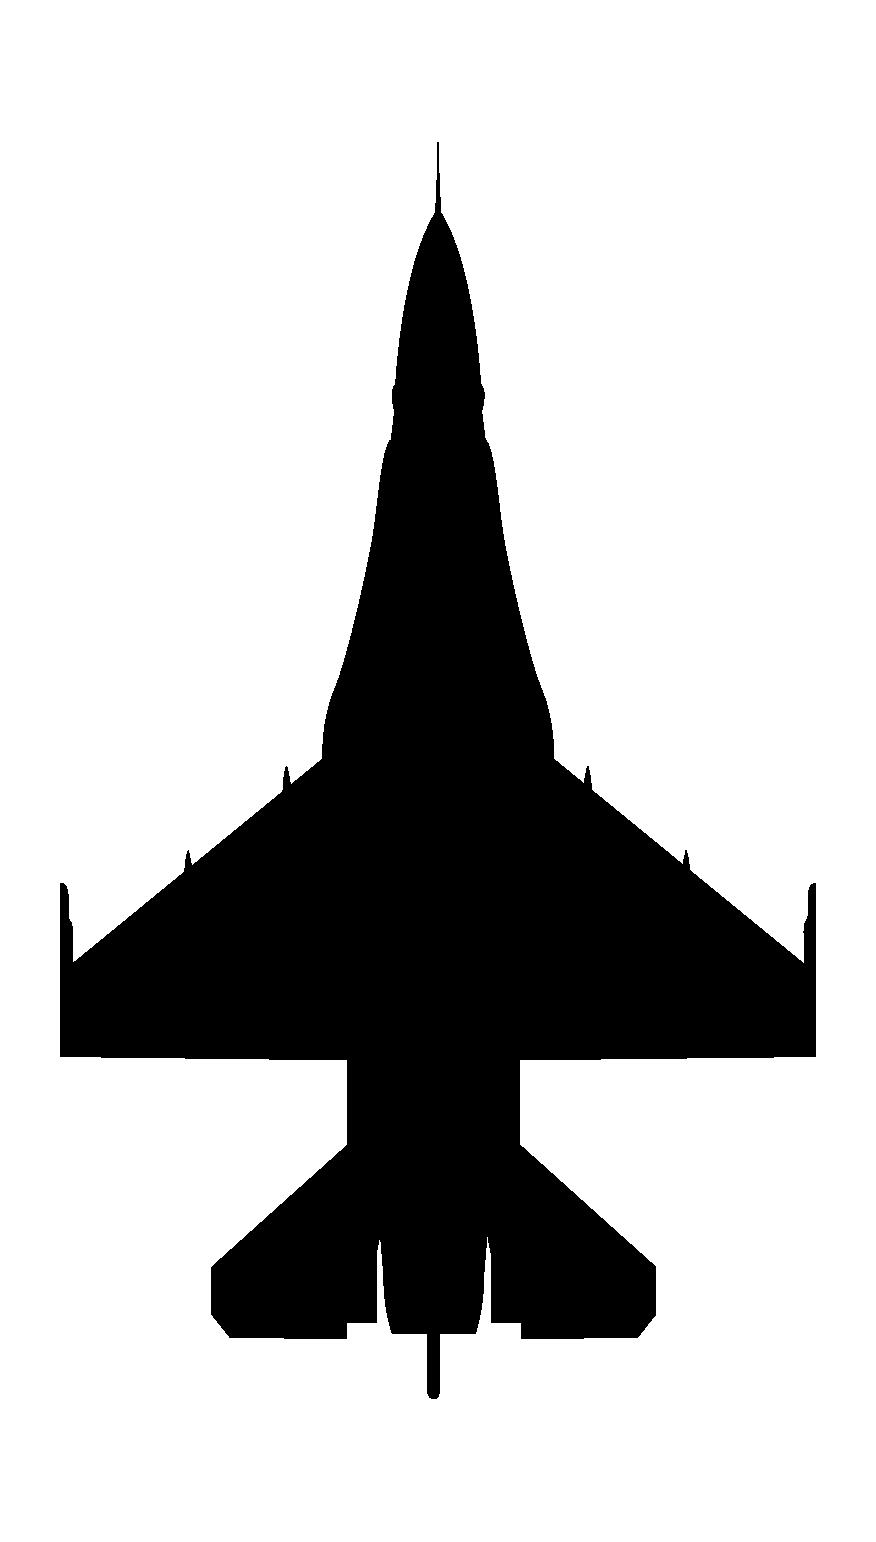
\includegraphics[
                height=15mm,
                angle=-90,
            ]{diagrams/aircraft/silhouette_f16_top.pdf}
        };

        \coordinate (offset) at (-3.5,0);
        \coordinate (center) at ($(offset)+(0:38)$);

        \draw[]
        (offset) -- node[pos=1, above right, font=\small\bfseries] {A6} +(60:30) arc (60:-60:30) -- cycle;
        \draw[]
        (offset) -- node[pos=1, above right, font=\small\bfseries] {A3} +(30:32) arc (30:-30:32) -- cycle;
        \draw[]
        (offset) -- +(25:34) arc (25:-25:34) -- node[pos=0, right, font=\small\bfseries] {A2} cycle;
        \draw[]
        (offset) -- node[pos=1, right, font=\small\bfseries] {A1} +(10:36) arc (10:-10:36) -- cycle;
        \draw[color2, fill=color2!20]
        (offset) -- +(1.5:38) arc (1.5:-1.5:38) -- cycle;

        \node[anchor=west, align=left, font=\small\bfseries, color2] at (center) {BEAMWIDTH};
    \end{tikzpicture}
    \caption{
        FCR azimuth scan \& limits. 
        Note that the A6 pattern scans the entire azimuth range of the radar.
        The varying radii for the different azimuth settings are for illustrative purposes.
    }
    \label{fig:sensors_aa:apg68:crm:azscan}
\end{figure}

\begin{figure}[htbp]
    \centering
    \begin{tikzpicture}[auto, node distance=10mm, x=1mm, y=1mm, very thick, line cap=round,
        >={Latex[round]}
        ]

        \node[
            anchor=east
        ] (mfd) at (0,0) {
            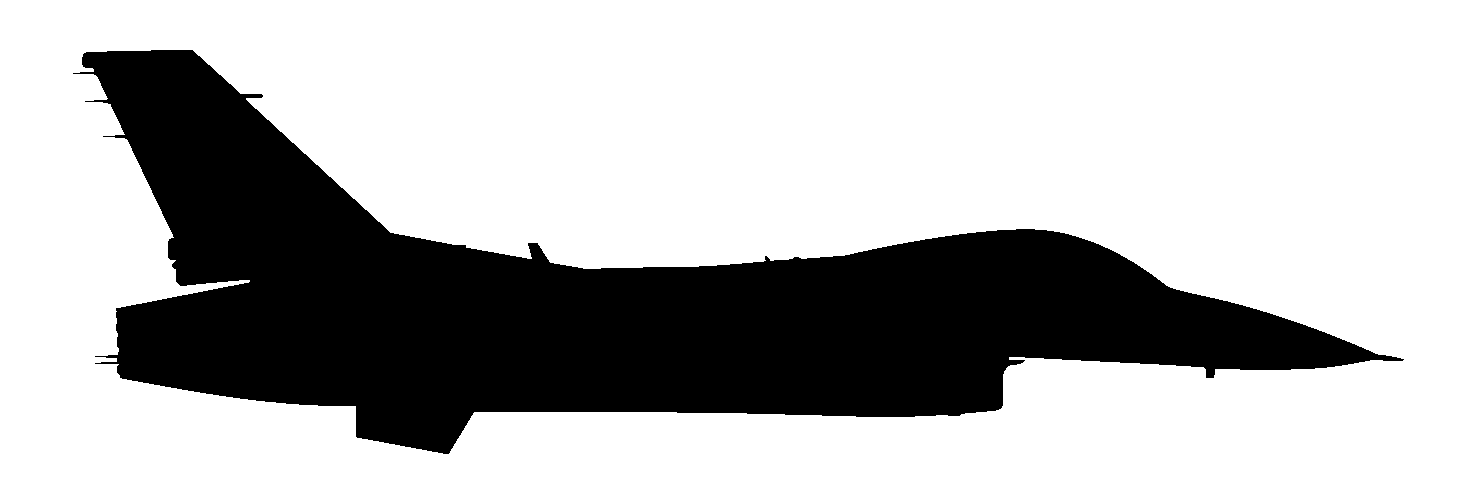
\includegraphics[
                width=15mm,
            ]{diagrams/aircraft/silhouette_f16_side.pdf}
        };

        \coordinate (offset) at (-2.5,-1);
        \coordinate (4bar) at ($(offset) + (36:35)$);
        \coordinate (3bar) at ($(offset) + (12:35)$);
        \coordinate (2bar) at ($(offset) + (-12:35)$);
        \coordinate (1bar) at ($(offset) + (-36:35)$);

        \node[font=\small\bfseries] at ($(4bar)+(5,2.5)$) {4B};
        \node[font=\small\bfseries] at ($(3bar)+(5,0)$) {3B};
        \node[font=\small\bfseries] at ($(2bar)+(5,0)$) {2B};
        \node[font=\small\bfseries] at ($(1bar)+(5,-2.5)$) {1B};

        \draw[]
        (offset) -- node[pos=1, above, font=\small\bfseries] {+/- 60 deg} +(60:35) arc (60:-60:35) -- cycle;
        \draw[color2, fill=color2!20]
        (offset) -- +(41.75:35) arc (41.75:31.25:35) -- cycle;
        \draw[color2, fill=color2!20]
        (offset) -- +(16.65:35) arc (16.65:7.35:35) -- cycle;
        \draw[color2, fill=color2!20]
        (offset) -- +(-8.45:35) arc (-8.45:-15.55:35) -- cycle;
        \draw[color2, fill=color2!20]
        (offset) -- +(-33.55:35) arc (-33.55:-38.45:35) -- cycle;

        \coordinate (4boffset) at ($(4bar) + (15,2.5)$);
        \coordinate (3boffset) at ($(3bar) + (15,0)$);
        \coordinate (2boffset) at ($(2bar) + (15,0)$);
        \coordinate (1boffset) at ($(1bar) + (15,-2.5)$);

        % 4bar
        \filldraw[color2!20] ($(4boffset) + (22.5,3.75)$) circle (2.5);

        \draw[->, rounded corners, ultra thick,]
        (4boffset)
        -- ($(4boffset) + (0,3.75)$)  -- ($(4boffset) + (20,3.75)$);
        \draw[->, rounded corners, ultra thick,]
        ($(4boffset) + (20,3.75)$)
        -- ($(4boffset) + (40,3.75)$) -- ++(0,-2.5)
        -- ++(-39,0) -- ++(0, -2.5)
        -- ++(39,0) -- ($(4boffset) + (+40,-3.75)$)
        -- ($(4boffset) + (20,-3.75)$);
        \draw[rounded corners, ultra thick,]
        ($(4boffset) + (20,-3.75)$)
        -- ($(4boffset) + (0,-3.75)$) 
        -- (4boffset);

        \draw[dashed, rounded corners=5]
        ($(4boffset) + (-2.5,6.25)$) -- ($(4boffset) + (42.5,6.25)$)
        -- ($(4boffset) + (42.5,-6.25)$) -- ($(4boffset) + (-2.5,-6.25)$)
        -- cycle;

        \draw[color2, ultra thick] ($(4boffset) + (22.5,3.75)$) circle (2.5);

        % 3bar
        \draw[->, rounded corners, ultra thick,]
        ($(3boffset) + (2.5,0)$) -- (3boffset)
        -- ($(3boffset) + (0,2.5)$) -- ($(3boffset) + (20,2.5)$);
        \draw[->, rounded corners, ultra thick,]
        ($(3boffset) + (20,2.5)$)
        -- ($(3boffset) + (40,2.5)$) -- ++(0,-2.5)
        -- ($(3boffset) + (20,0)$);
        \draw[->, rounded corners, ultra thick,]
        ($(3boffset) + (20,0)$)
        -- ($(3boffset) + (0,0)$) -- ++(0, -2.5)
        -- ($(3boffset) + (+20,-2.5)$);
        \draw[rounded corners, ultra thick,]
        ($(3boffset) + (+20,-2.5)$)
        -- ($(3boffset) + (+40,-2.5)$) -- ++(0,2.5)
        -- ($(3boffset) + (2.5,0)$);

        \draw[dashed, rounded corners=5]
        ($(3boffset) + (-2.5,5)$) -- ($(3boffset) + (42.5,5)$)
        -- ($(3boffset) + (42.5,-5)$) -- ($(3boffset) + (-2.5,-5)$)
        -- cycle;

        % 2bar
        \draw[->, rounded corners, ultra thick,]
        (2boffset)
        -- ($(2boffset) + (0,1.25)$) -- ($(2boffset) + (20,1.25)$);
        \draw[->, rounded corners, ultra thick,]
        ($(2boffset) + (20,1.25)$)
        -- ($(2boffset) + (40,1.25)$)
        -- ($(2boffset) + (40,-1.25)$) -- ($(2boffset) + (20,-1.25)$);
        \draw[rounded corners, ultra thick,]
        ($(2boffset) + (20,-1.25)$)
        -- ($(2boffset) + (0,-1.25)$)
        -- (2boffset);

        \draw[dashed, rounded corners=5]
        ($(2boffset) + (-2.5,3.75)$) -- ($(2boffset) + (42.5,3.75)$)
        -- ($(2boffset) + (42.5,-3.75)$) -- ($(2boffset) + (-2.5,-3.75)$)
        -- cycle;

        % 1bar
        \draw[->, rounded corners, ultra thick,]
        ($(1boffset) + (0,0)$) -- ($(1boffset) + (15,0)$);
        \draw[->, rounded corners, ultra thick,]
        ($(1boffset) + (40,0)$) -- ($(1boffset) + (25,0)$);
        \draw[rounded corners, ultra thick,]
        ($(1boffset) + (25,0)$) -- ($(1boffset) + (0,0)$);

        \draw[dashed, rounded corners=5]
        ($(1boffset) + (-2.5,2.5)$) -- ($(1boffset) + (42.5,2.5)$)
        -- ($(1boffset) + (42.5,-2.5)$) -- ($(1boffset) + (-2.5,-2.5)$)
        -- cycle;
    \end{tikzpicture}
    \caption{
        FCR elevation scan \& limits. 
        The radar beam --- blue circle --- tracks along the illustrated scan pattern in a loop, resulting in the dashed scan volume. 
        Note that the scan patterns are not drawn to scale.
    }
    \label{fig:sensors_aa:apg68:crm:barscan}
\end{figure}

\clearpage

\subsubsection{MFD CONTROLS}

\begin{tcoloritemize}
    \blueitem{Radar Mode}{
    \textbf{OSB 1} opens page allowing selection of radar mode

    \begin{subitemize}
        \item \textbf{Left Side (OSB 19-20)} --- A-A Modes
        \begin{itemize}
            \item CRM --- see \cref{subsec:crm}
            \item ACM --- see \cref{subsec:acm}
        \end{itemize}
        \item \textbf{Right Side (OSB 6-9)} --- A-G Modes
        \begin{itemize}
            \item See \cref{sec:fcr-ag}
        \end{itemize}
        \item \textbf{STBY (OSB 10)} --- places FCR in standby
    \end{subitemize}}
    \blueitem{Field of View}{
    \textbf{OSB 3} cycles field of view

    \begin{subitemize}
        \item \textbf{EXP} --- expanded field of view
        \item \textbf{NORM} --- normal field of view
    \end{subitemize}

    HOTAS \textbf{EXPAND/FOV} switch also cycles FOV}
    \blueitem{Override}{Pressing \textbf{OVRD (OSB 4)}  places FCR in standby}
    \blueitem{FCR Control}{\textbf{CNTL (OSB 5)} opens FCR control page}
    \blueitem{Datalink Mode}{\textbf{OSB 6} cycles datalink operating mode (WIP)}
    \blueitem{Declutter}{\textbf{DCLT (OSB 11)} opens FCR declutter page, allowing pilot to deselect symbology elements}
    \blueitem{Elevation Bar \break Select}{\textbf{OSB 17} cycles elevation bar search pattern}
    \blueitem{Azimuth Select}{
    \textbf{OSB 18} cycles azimuth search pattern}
    \blueitem{Range Select}{
    \textbf{OSB 19-20} adjusts FCR display range scale
    
    \begin{subitemize}
        \item \textbf{Can be cycled by ``walking'' cursor off top/bottom of display}
    \end{subitemize}
    }
\end{tcoloritemize}

\notebox{
    \textbf{Azimuth and range can also be cycled by ``walking'' acquisition cursor of side of FCR display}
}

\begin{figure}[htbp]
    \centering
    \begin{tikzpicture}[auto, node distance=10mm, x=1mm, y=1mm, very thick, line cap=round,
        >={Latex[round]}
        ]
        
        \node[] (fig) at (0,0) {
            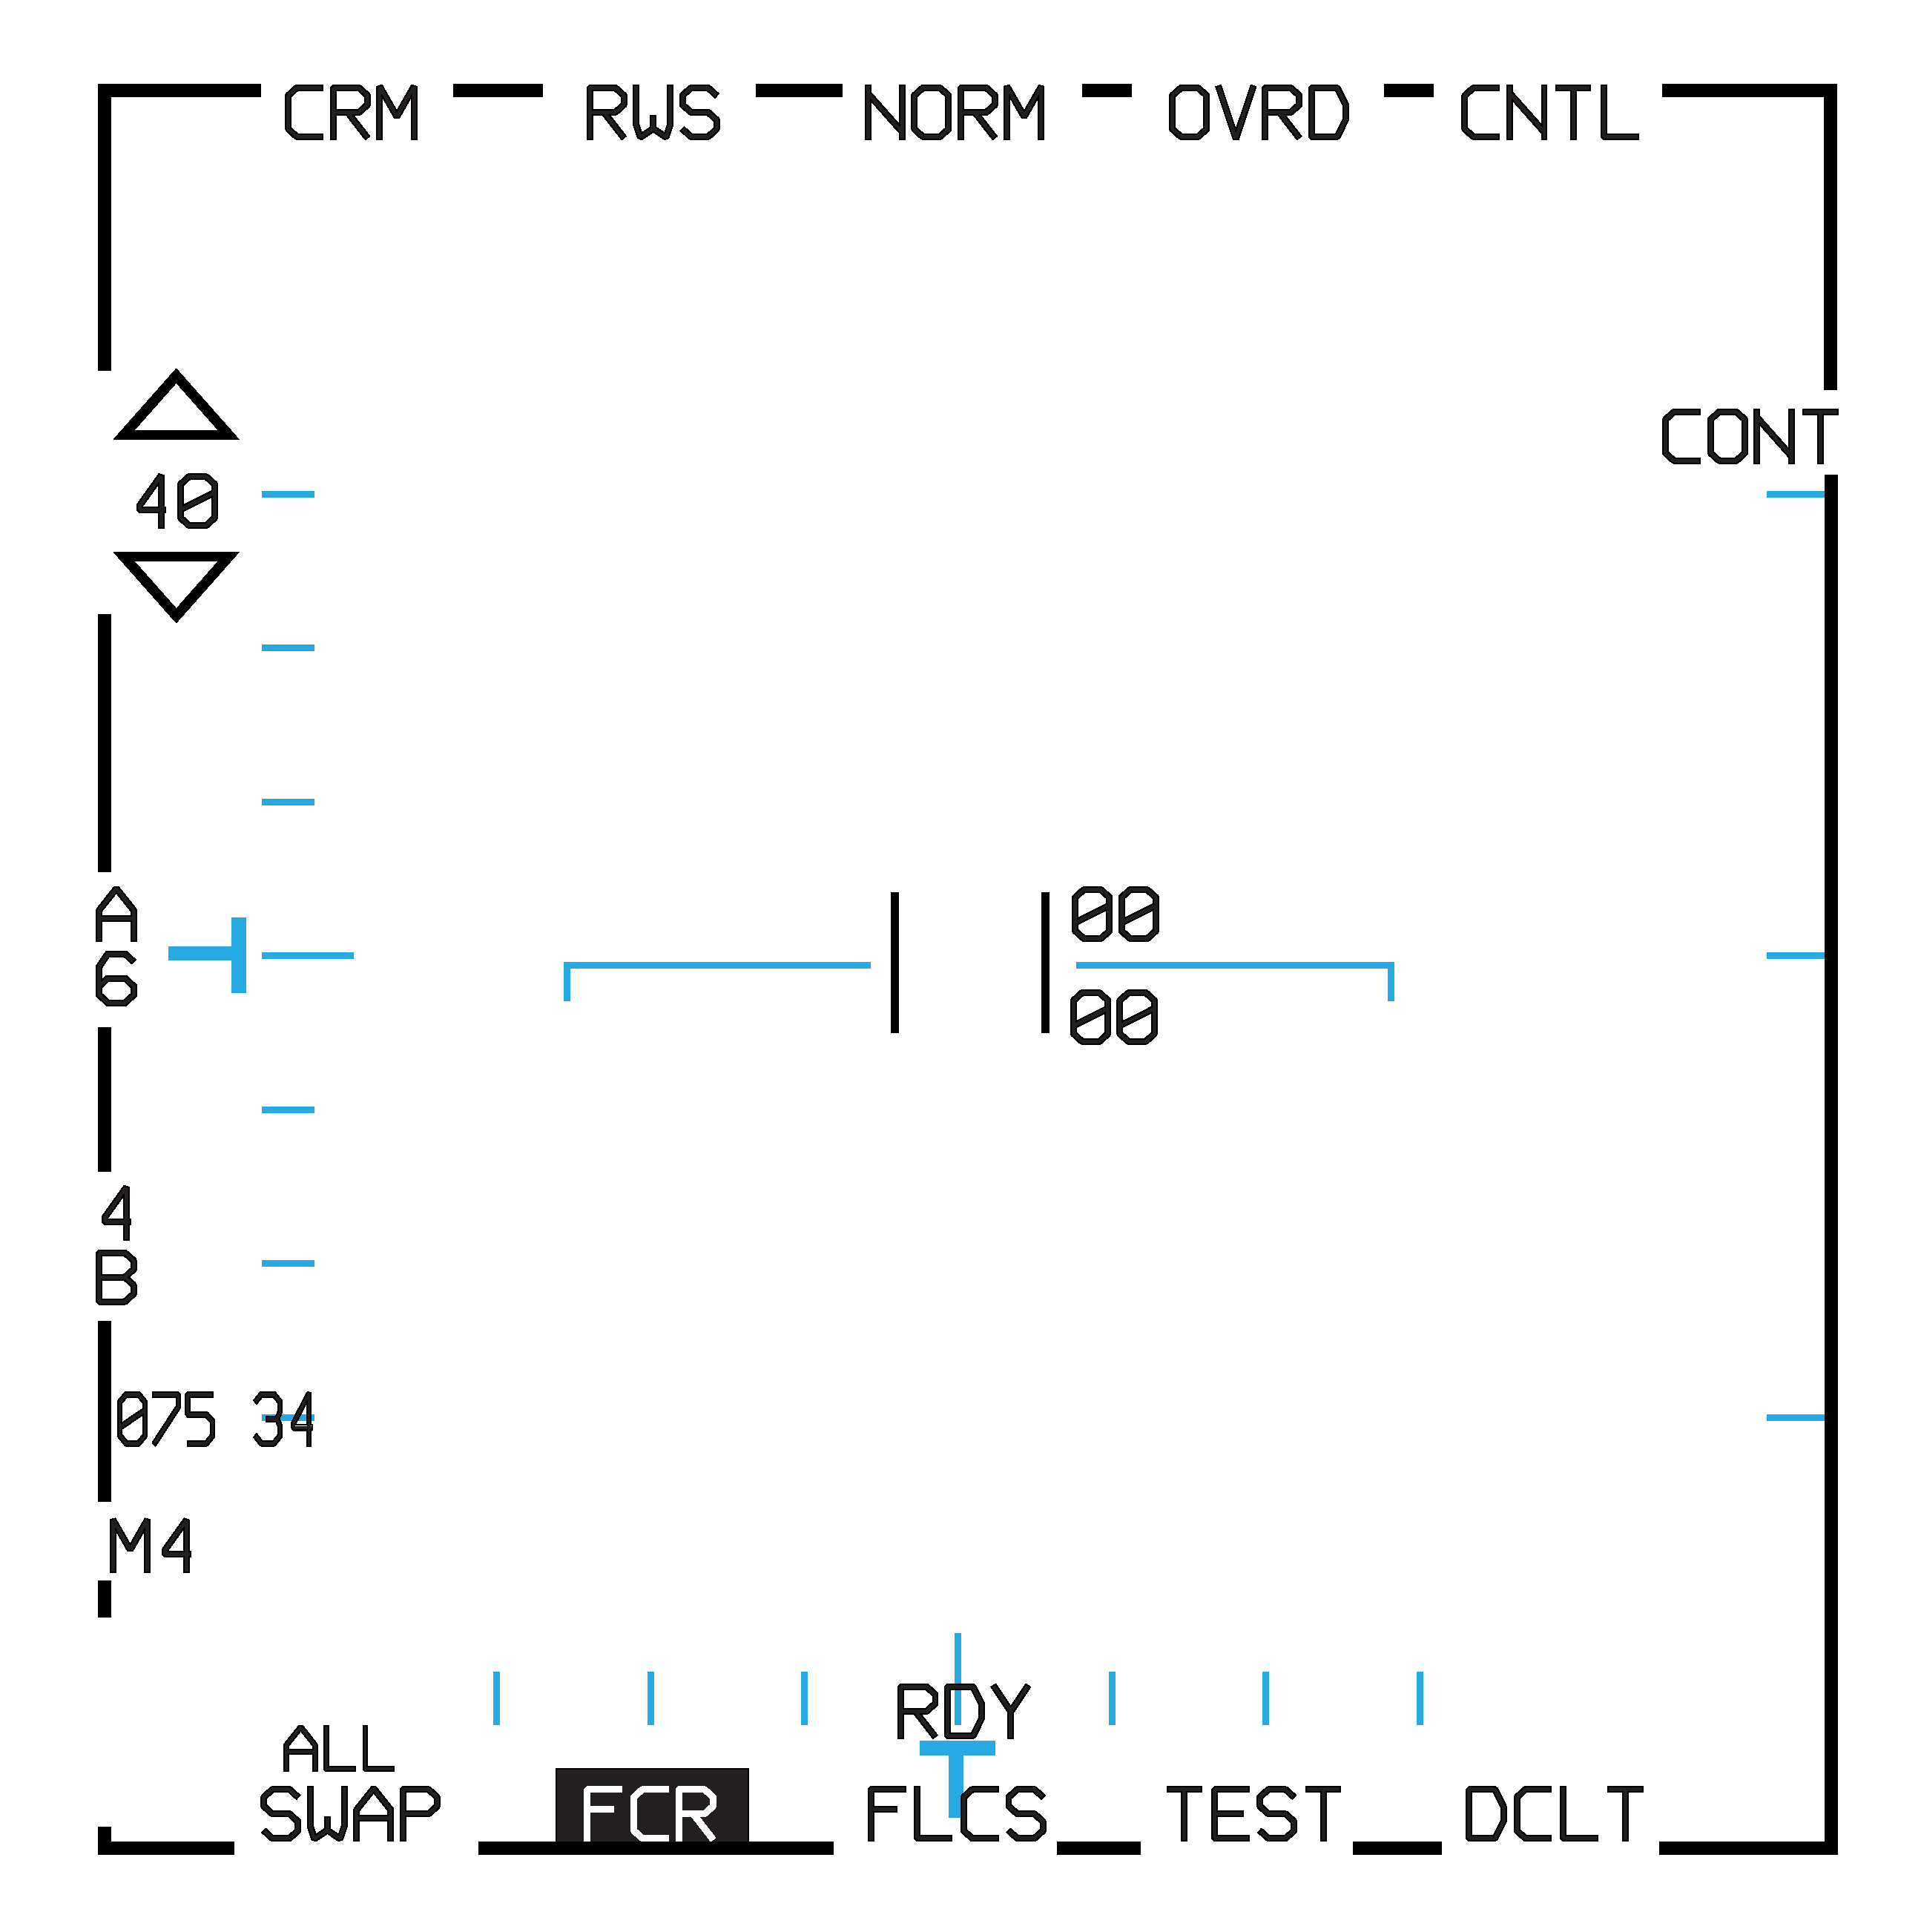
\includegraphics[
                height=75mm,
            ]{mfd/fcr_aa/rws_homepage.pdf}
        };

        % Annotations
        \node[lannot] (mode) at ($(fig.west)+(0mm,38mm)$) {FCR mode};
        \draw[->, red] (mode.east) -- ++(12mm, 0mm) -- (-24mm,35mm);

        \node[lannot] (submode) at ($(fig.west)+(0mm,28mm)$) {CRM \\ submode};
        \draw[->, red] (submode.east) -- ++(23mm, 0mm) -- (-13mm, 31mm);

        \node[lannot] (rsel) at ($(fig.west)+(0mm,18mm)$) {Range select};
        \draw[->, red] (rsel.east) -- ++(4.5mm, 0mm);

        \node[lannot] (asel) at ($(fig.west)+(0mm,0.5mm)$) {Azimuth select};
        \draw[->, red] (asel.east) -- ++(4.5mm, 0mm);

        \node[lannot] (bsel) at ($(fig.west)+(0mm,-10.5mm)$) {Elevation bar select};
        \draw[->, red] (bsel.east) -- ++(4.5mm, 0mm);

        \node[annot, anchor=south, align=center] (fov) at ($(fig.north)+(0mm,0mm)$) {FOV select};
        \draw[->, red] (fov.south) -- ++(0mm, -3.5mm);

        \node[rannot] (cntl) at ($(fig.east)+(0mm,38mm)$) {Control};
        \draw[->, red] (cntl.west) -- ++(-13mm, 0mm) -- (23mm, 35mm);

        \node[rannot] (ovrd) at ($(fig.east)+(0mm,28mm)$) {Override};
        \draw[->, red] (ovrd.west) -- ++(-24mm, 0mm) -- (12mm, 31mm);

        \node[rannot] (dl) at ($(fig.east)+(0mm,20.5mm)$) {Datalink mode};
        \draw[->, red] (dl.west) -- ++(-4mm,0mm);

        \node[rannot] (acq) at ($(fig.east)+(0mm,10mm)$) {Acquisition cursor};
        \draw[->, red] (acq.west) -- ++(-30mm, 0mm) -- (3mm,5mm);

        \node[rannot] (sj) at ($(fig.east)+(0mm,-8mm)$) {Horizon \\indicator};
        \draw[->, red] (sj.west) -- ++(-20mm, 0mm) -- (12mm,-1mm);

        \node[rannot] (dclt) at ($(fig.east)+(0mm,-38mm)$) {Declutter};
        \draw[->, red] (dclt.west) -- ++(-13mm, 0mm) -- (23mm, -35mm);
    \end{tikzpicture}
    \caption{FCR page with basic controls \& symbology marked. Note that FCR is illustrated in default mode immediately after startup.}
\end{figure}

\clearpage

\subsection{RWS}
\label{subsec:rws}
\begin{tcoloritemize}
    \blueitem[RWS]
    \textbf{R}ange \textbf{W}hile \textbf{S}earch

    \begin{itemize}
        \item \textbf{Fast, Long(er)-Range Search}
        \begin{itemize}
            \item radar scans selectable search volume
            \item displays raw target position returns
        \end{itemize}
        \item \textbf{No track data} 
        \begin{itemize}
            \item exact target range, velocity, angle, etc.
            \item but can transition to advanced modes
        \end{itemize}
        % (exact target range, velocity, angle, etc.)
        % --- but can transition to advanced modes
    \end{itemize}
\end{tcoloritemize}

\begin{figure}[htbp]
    \centering
    \begin{tikzpicture}[auto, node distance=10mm, x=1mm, y=1mm, very thick, line cap=round,
        >={Latex[round]}
        ]
        
        \node[] (fig) at (0,0) {
            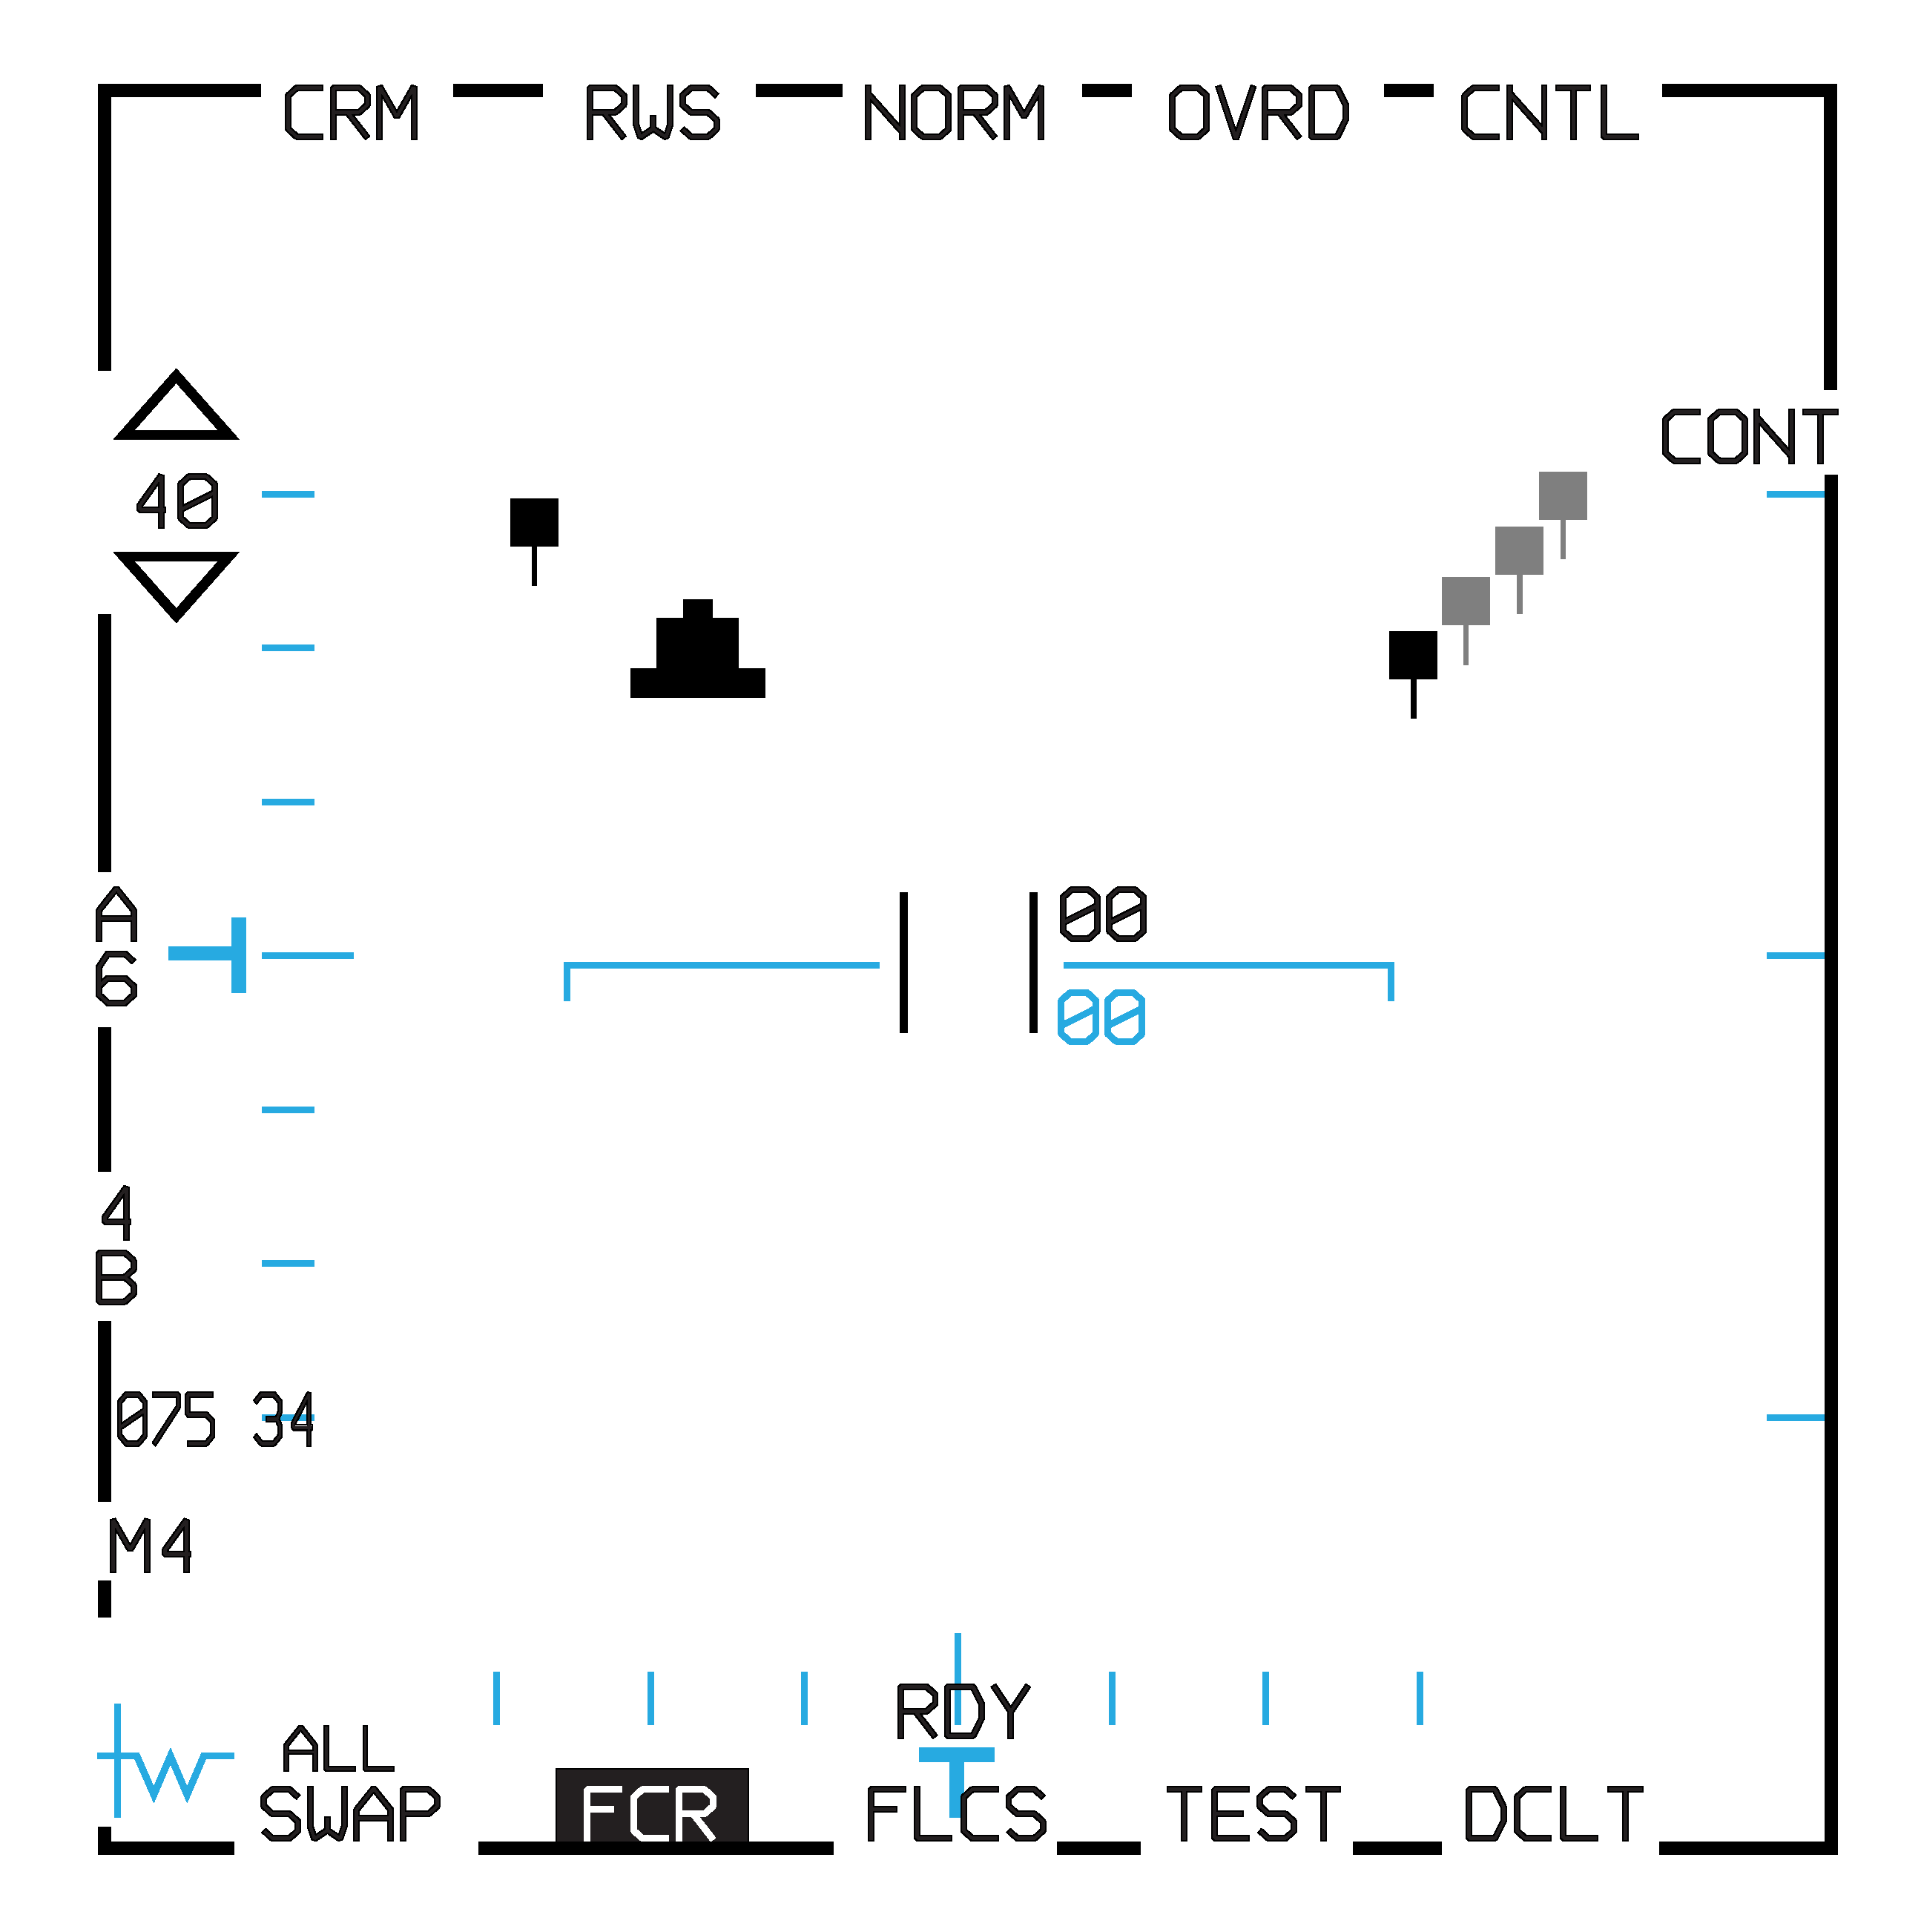
\includegraphics[
                height=75mm,
            ]{mfd/fcr_aa/rws_search.pdf}
        };

        % Annotations
        \node[lannot] (rsel) at ($(fig.west)+(0mm,18mm)$) {Range select};
        \draw[annotptr] (rsel.east) -- ++(4.5mm, 0mm);

        \node[lannot] (asel) at ($(fig.west)+(0mm,0.5mm)$) {Azimuth select};
        \draw[annotptr] (asel.east) -- ++(4.5mm, 0mm);

        \node[lannot] (bsel) at ($(fig.west)+(0mm,-10.5mm)$) {Elevation bar select};
        \draw[annotptr] (bsel.east) -- ++(4.5mm, 0mm);

        \node[rannot] (ret) at ($(fig.east)+(0mm,28mm)$) {RWS \\ returns};
        \draw[annotptr] (ret.west) -- ++(-16mm, 0mm) -- (18mm,18mm);
        \draw[annotptr] (ret.west) -- ++(-50mm, 0mm) -- (-16mm,20mm);

        \node[rannot] (stpt) at ($(fig.east)+(0mm,6mm)$) {Current STPT};
        \draw[annotptr] (stpt.west) -- ++(-42mm, 0mm) -- (-7mm,9mm);

        \node[rannot] (acq) at ($(fig.east)+(0mm,-10mm)$) {Acquisition cursor};
        \draw[annotptr] (acq.west) -- ++(-30mm, 0mm) -- (3mm,-5mm);
    \end{tikzpicture}
    \caption{RWS FCR mode symbology.}
\end{figure}

\begin{tcoloritemize}
    \blueitem[SAM \break Submode]
    \textbf{S}ituational \textbf{A}warness \textbf{M}ode

    \begin{itemize}
        \item \textbf{Target is ``Bugged''} (Pseudo-Track)
        \begin{itemize}
            \item can guide AIM-120C (w/o STT Lock)
            \item DLZ displayed if missile selected
        \end{itemize}
        \item \textbf{RWS search  continues}
        \begin{itemize}
            \item scan pauses on SAM target
            \item FCR manages scan volume
        \end{itemize}
    \end{itemize}
    \blueitem[DTT \break Submode]
    \textbf{D}ual \textbf{T}arget \textbf{T}rack

    \begin{itemize}
        \item \textbf{2 Targets ``Bugged''} --- primary / secondary
        \begin{itemize}
            \item can guide AIM-120C on \textbf{\underline{primary target}}
            \item DLZ displayed if missile selected
        \end{itemize}
        \item \textbf{TMS Left --- swaps primary / secondary}
        \item \textbf{RWS search  continues}
        \begin{itemize}
            \item scan pauses on both primary / secondary
            \item FCR manages scan volume
        \end{itemize}
        \item \textbf{Within 10nm search pattern inhibited} --- radar only scans primary/secondary targets
        \item \textbf{Once \underline{either} target within 3nm automatically transitions to STT}
    \end{itemize}
    \blueitem[Spotlight]
        
    \textbf{Narrow scan centered on acquisition cursor}
    \begin{itemize}
        \item \textbf{Narrow scan}
        \begin{itemize}
            \item 4 bar elevation 
            \item \pm10 deg azimuth
        \end{itemize}
        \item Useful to rapidly acquire radar returns from target at known position
        \item \textbf{Activated by holding TMS Forward >1 sec}
        \begin{itemize}
            \item enters SAM submode if target detected under Acquisition Cursor
            \item returns to previous search pattern if no target under Acquisition Cursor when released
        \end{itemize}
    \end{itemize}
\end{tcoloritemize}

\begin{figure}[htbp]
    \centering
    \begin{tikzpicture}[auto, node distance=10mm, x=1mm, y=1mm, very thick, line cap=round,
        >={Latex[round]}
        ]
        
        \node[] (fig) at (0,0) {
            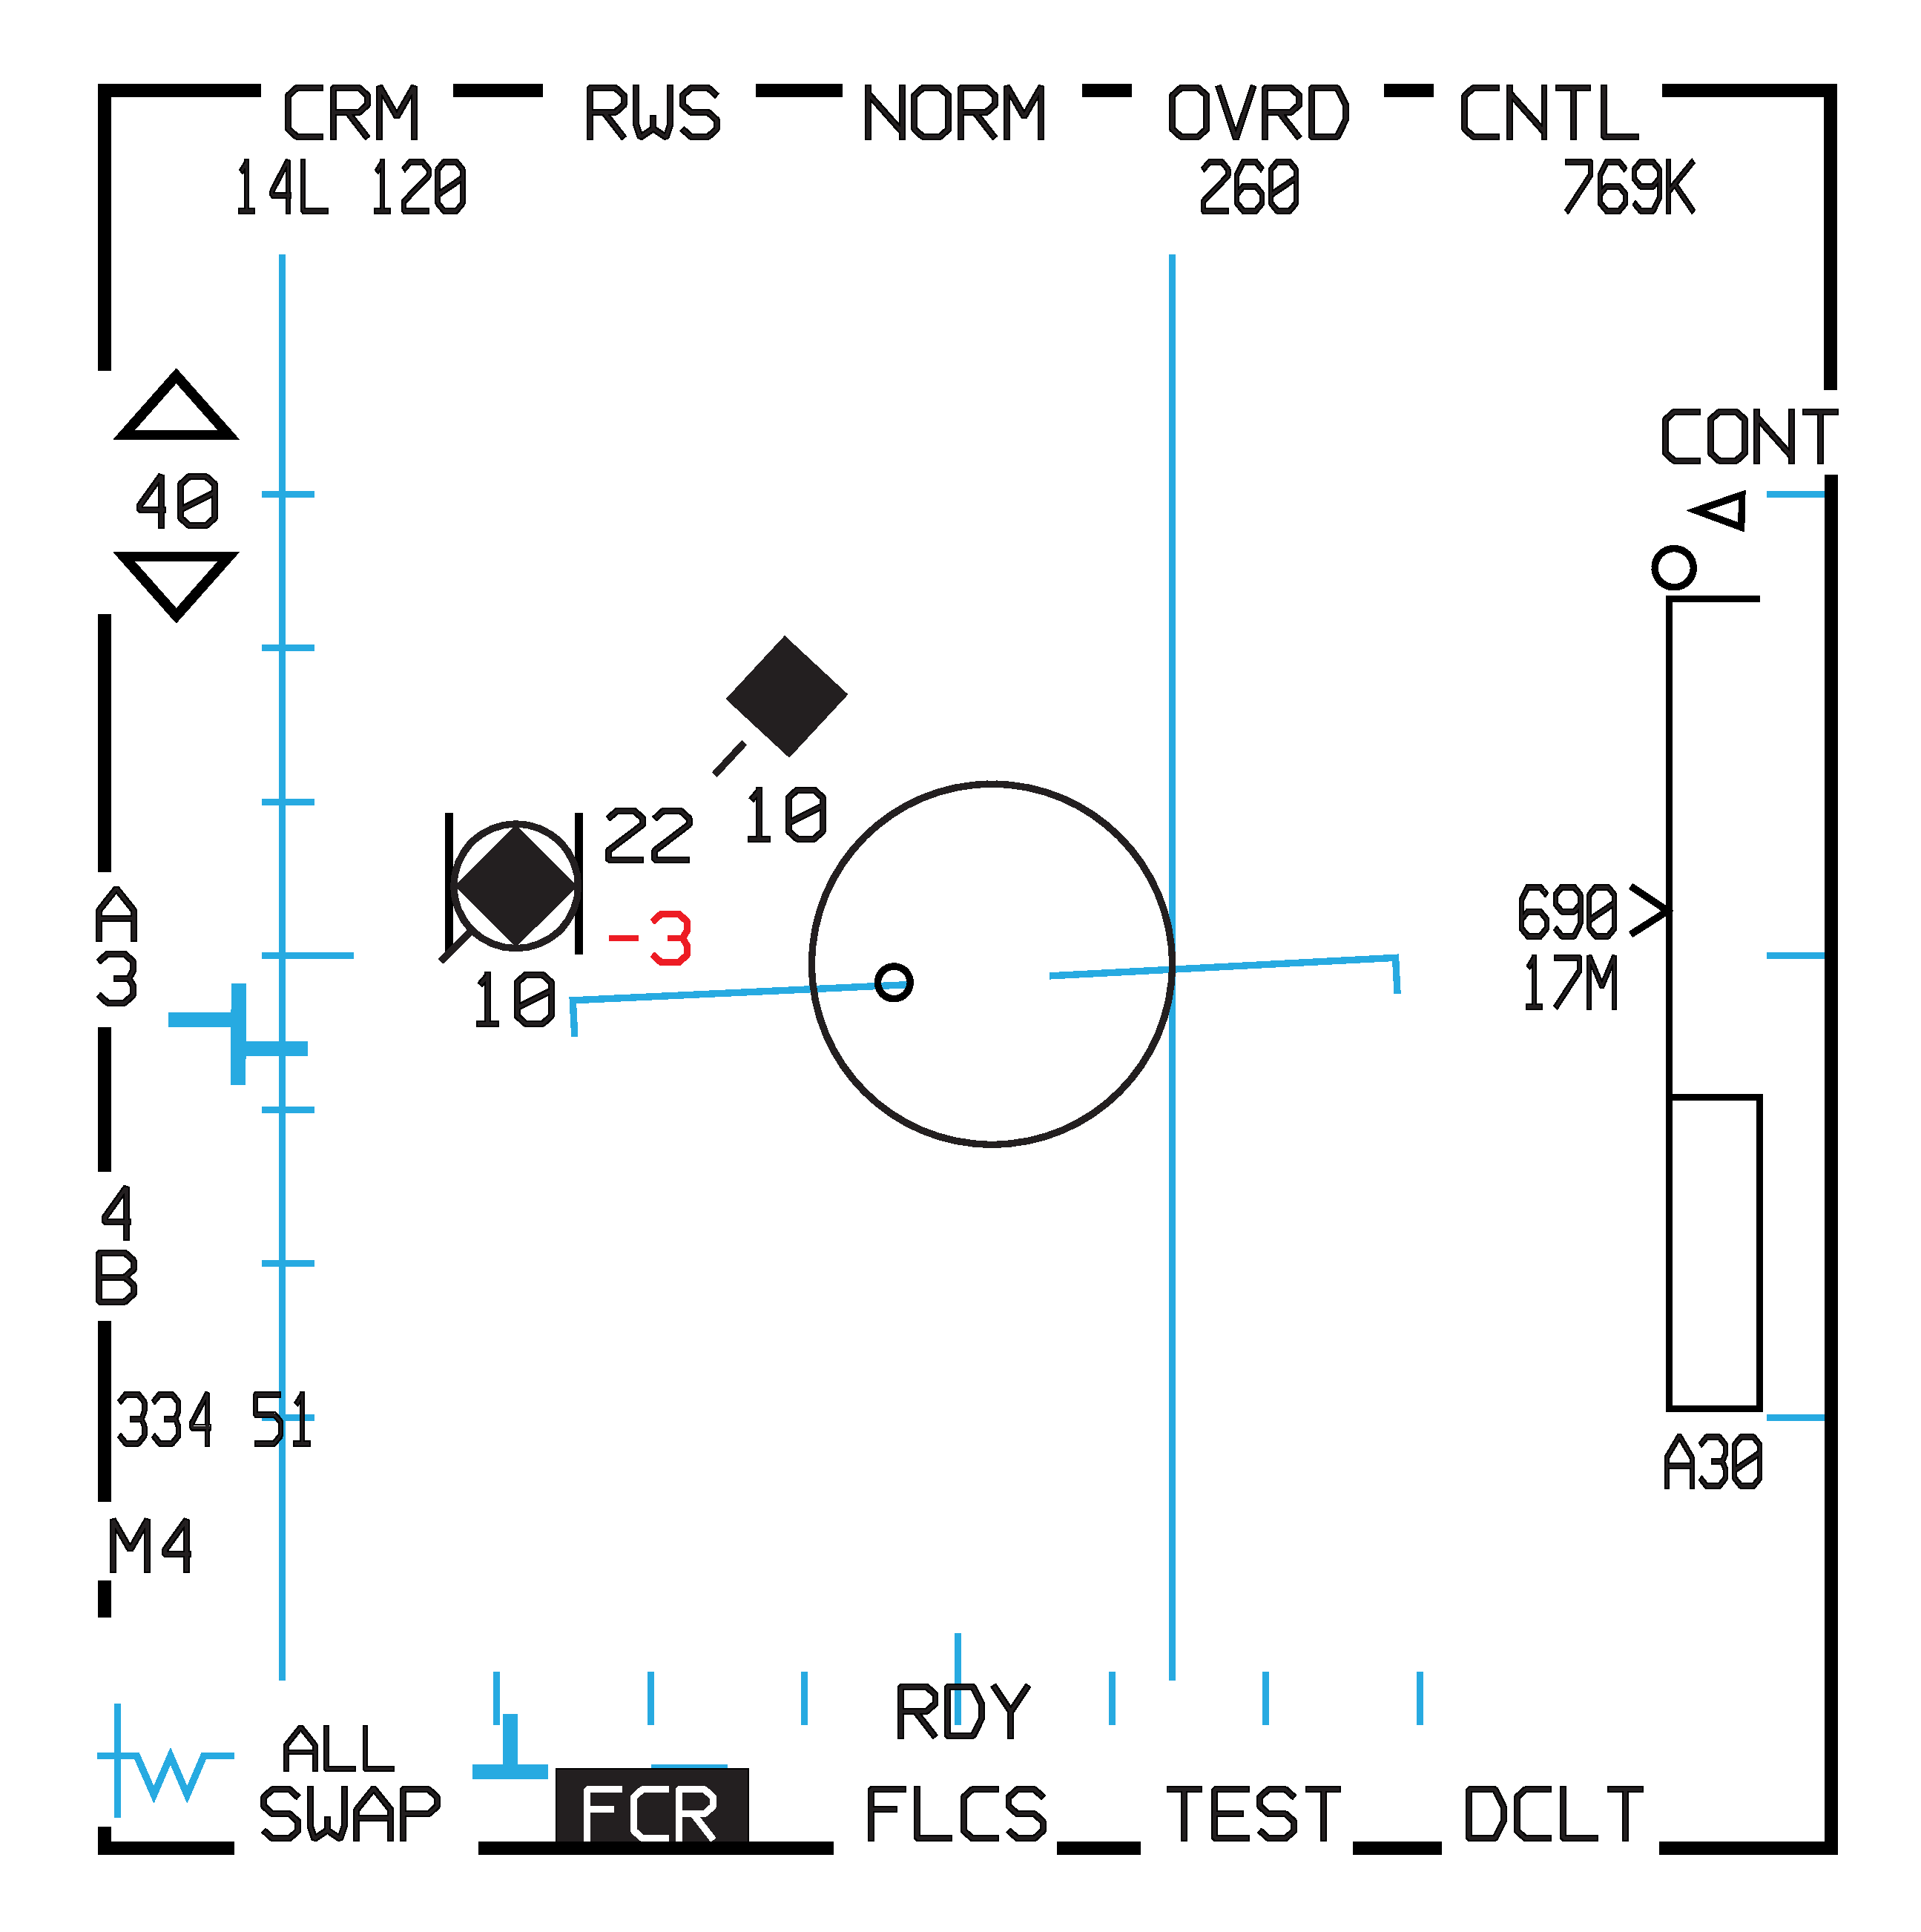
\includegraphics[
                height=75mm,
            ]{mfd/fcr_aa/rws_sam_dtt.pdf}
        };

        % Annotations
        \node[lannot] (asp) at ($(fig.west)+(0mm,30.25mm)$) {Aspect};
        \draw[annotptr] (asp.east) -- ++(9mm, 0mm);

        \node[lannot] (trk) at ($(fig.west)+(0mm,24mm)$) {Track};
        \draw[annotptr] (trk.east) -- ++(12mm, 0mm) -- ++(4mm, 4mm);

        \node[lannot] (sec) at ($(fig.west)+(0mm,10.25mm)$) {Secondary target};
        \draw[annotptr] (sec.east) -- ++(27mm, 0mm);

        \node[lannot] (prim) at ($(fig.west)+(0mm,-7mm)$) {Primary target \& cursor};
        \draw[annotptr] (prim.east) -- ++(15mm, 0mm) -- ++(4mm, 6mm);

        \node[rannot] (clos) at ($(fig.east)+(0mm,30.25mm)$) {Closure};
        \draw[annotptr] (clos.west) -- ++(-9mm, 0mm);

        \node[rannot] (as) at ($(fig.east)+(0mm,24mm)$) {Airspeed};
        \draw[annotptr] (as.west) -- ++(-22mm, 0mm) -- ++(-4mm, 4mm);

        \node[rannot] (dlz) at ($(fig.east)+(0mm,-2mm)$) {DLZ \\ {\footnotesize see \cref{fig:aa_weap:aim120:dlz}}};
        \draw[annotptr] (dlz.west) -- ++(-8mm, 0mm);

        \node[rannot] (asec) at ($(fig.east)+(0mm,-24mm)$) {ASC / ASEC \\ {\footnotesize see \cref{fig:aa_weap:aim120:asc_asec}}};
        \draw[annotptr] (asec.west) -- ++(-26mm, 0mm) -- (4mm,-7mm);

        \node[annot, anchor=south, align=left, text width=35mm] (fov) at ($(fig.north)+(-6.5mm,0mm)$) {Azimuth scan limits};
        \draw[annotptr] (fov.south) -- ++(0mm, -15mm) -- ++(12mm, -6mm);
    \end{tikzpicture}
    \caption{RWS SAM / DTT submode symbology. Additional information on primary target is displayed at top of FCR page.}
\end{figure}

\marginfigeometry

\subsubsection{SELECT RWS MODE}
\begin{checklistenumerate}
    \blueitem[FCR Switch] \textbf{FCR}
    \blueitem[Desired MFD] \textbf{FCR Page}, verify \textbf{SOI}
    \blueitem[Radar Mode]
        \textbf{CRM} (default), verify

        \begin{itemize}
            \item \textbf{Dogfight/Missile Override} --- \textbf{NORM}
            \item \textbf{Radar Mode (OSB 1)} --- shows \textbf{CRM}
        \end{itemize}
    \blueitem[CRM Submode]
        \textbf{RWS} (default), cycle via 

        \begin{itemize}
            \item \textbf{TMS Right (long)} / \textbf{OSB 2} 
        \end{itemize}
\end{checklistenumerate}

\subsubsection{SAM / DTT ACQUISITION}
\label{subsec:rws:samdttacq}
\begin{checklistenumerate}
    \blueitem[Locate Targets]
    \begin{enumerate}
        \item Correlate onboard/offboard sensors
        \begin{itemize}
            \item raw radar returns, RWR pings
            \item AWACS calls, datalink targets
        \end{itemize}
        \item Place targets within radar scan volume
    \end{enumerate}
    \blueitem[SAM Acquisition]
    \marginpar{
        \captionsetup{type=figure}
        \centering
        \begin{tikzpicture}[figstyle]
            
            \node[boxedmarfigstyle] (search) at (0,0) {
                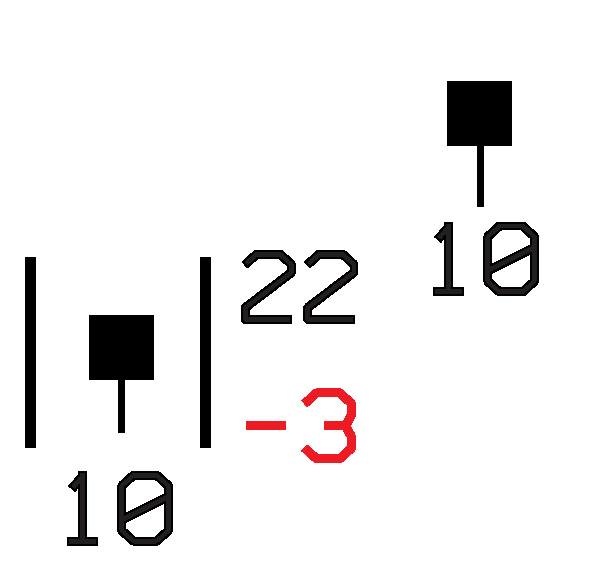
\includegraphics[
                    scale=0.25,
                ]{mfd/fcr_aa/rws_sam_dtt_subfig_01.pdf}
            };
            \node[boxedmarfigstyle] (sam) at (0,-35) {
                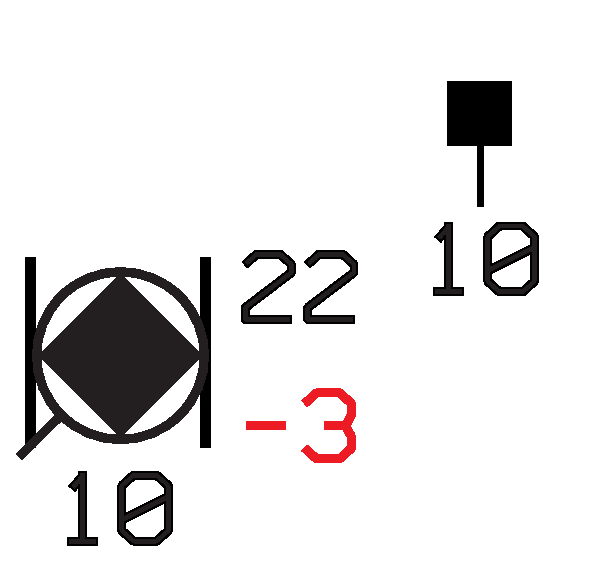
\includegraphics[
                    scale=0.25,
                ]{mfd/fcr_aa/rws_sam_dtt_subfig_02.pdf}
            };

            \draw[->]
            (search) -- node[right, align=center, font=\small] {\textbf{TMS} \textbf{FWD}}(sam);
        \end{tikzpicture}
        \caption{SAM Acquisition}
    }
    \begin{enumerate}
        \item \textbf{Target} \dotfill under Acquisition Cursor
        \item \textbf{TMS} \dotfill \textbf{Forward (hold)}
        \item \textbf{Target} \dotfill Verify \textbf{Bugged}
    \end{enumerate}
    \begin{itemize}
        \item Can guide AIM-120C on Bugged target
        \item DLZ displayed if missile selected
        \item RWS search continues
    \end{itemize}
    \blueitem[DTT Acquisition] (if desired)
    \marginpar{
        \captionsetup{type=figure}
        \centering
        \begin{tikzpicture}[figstyle]
            
            \node[boxedmarfigstyle] (sam) at (0,0) {
                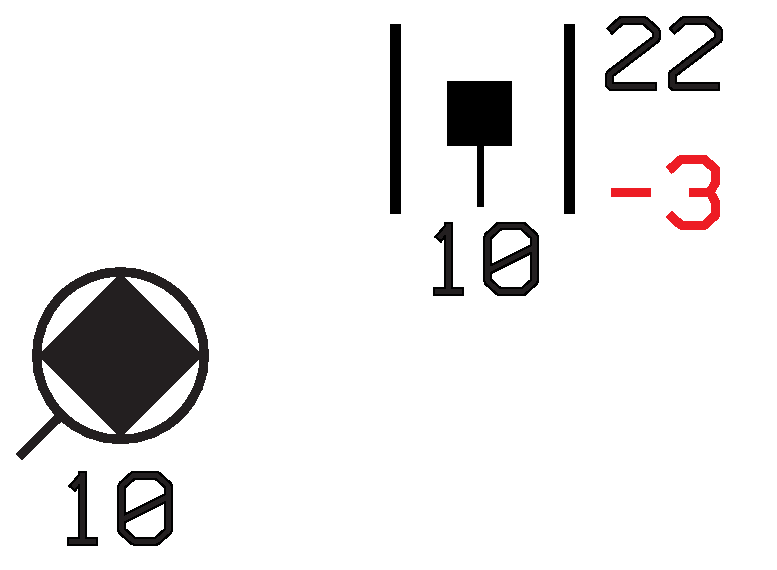
\includegraphics[
                    scale=0.25,
                ]{mfd/fcr_aa/rws_sam_dtt_subfig_03.pdf}
            };
            \node[boxedmarfigstyle] (dtt) at (0,-35) {
                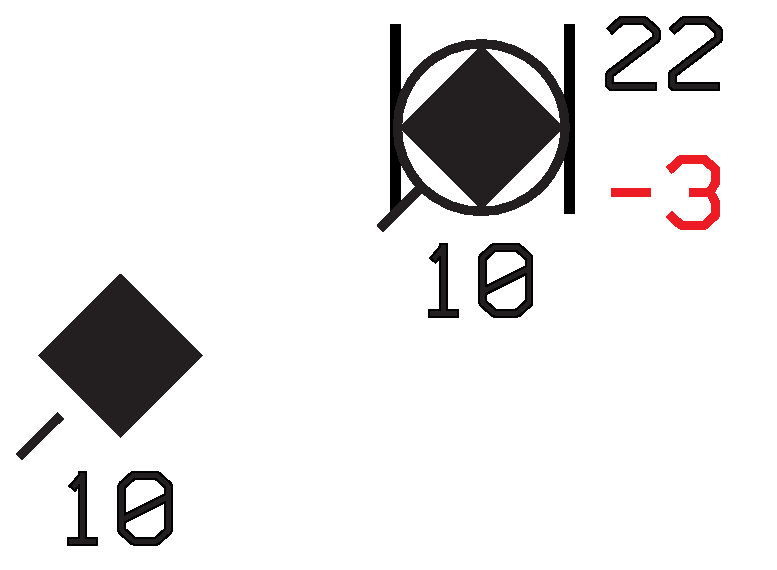
\includegraphics[
                    scale=0.25,
                ]{mfd/fcr_aa/rws_sam_dtt_subfig_04.pdf}
            };

            \draw[->]
            (sam) -- node[right, align=center, font=\small] {\textbf{TMS} \textbf{FWD}}(dtt);
        \end{tikzpicture}
        \caption{DTT Acquisition}
    }
    \begin{enumerate}
        \item \textbf{Target 2} \dotfill under Acquisition Cursor
        \item \textbf{TMS} \dotfill \textbf{Forward (hold)}
    \end{enumerate}

    To swap primary / secondary target

    \begin{enumerate}[start=3]
        \item \textbf{TMS} \dotfill \textbf{Left}
    \end{enumerate}
    \blueitem[STT Lock] (if desired)
    \begin{enumerate}
        \item \textbf{Target} \dotfill under Acquisition Cursor
        \item \textbf{TMS} \dotfill \textbf{Forward}
    \end{enumerate}
\end{checklistenumerate}

\subsubsection{SPOTLIGHT ACQUISITION}
\begin{checklistenumerate}
    \blueitem[Locate Targets]
    \begin{enumerate}
        \item Correlate onboard/offboard sensors
        \begin{itemize}
            \item raw radar returns, RWR pings
            \item AWACS calls, datalink targets
        \end{itemize}
        \item Place target within radar scan limits
    \end{enumerate}
    \blueitem[Spotlight Search]
    \marginpar{
        \captionsetup{type=figure}
        \centering
        \begin{tikzpicture}[figstyle]
            
            \node[
                boxedmarfigstyle,            
            ] (cursoroff) at (0,0) {
                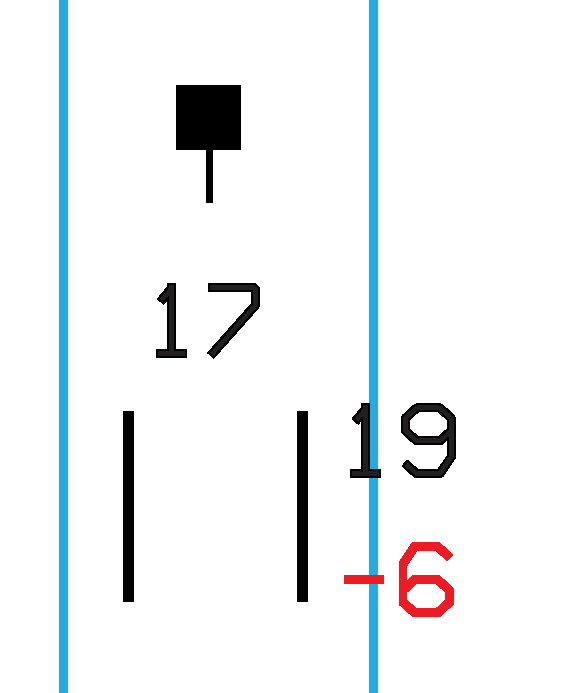
\includegraphics[
                    scale=0.25,
                ]{mfd/fcr_aa/rws_spotlight_subfig_cursor_off.pdf}
            };
            \node[
                boxedmarfigstyle,                
                below=10 of cursoroff,
            ] (cursoron) {
                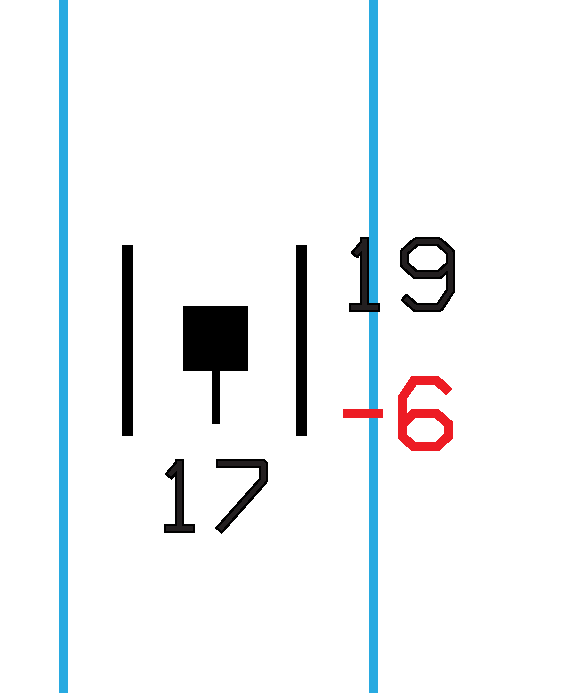
\includegraphics[
                    scale=0.25,
                ]{mfd/fcr_aa/rws_spotlight_subfig_cursor_on.pdf}
            };
            \node[
                boxedmarfigstyle,                
                below=10 of cursoron,
            ] (bugged) {
                
\includegraphics[
                    scale=0.5,
                ]{mfd/fcr_aa/tgt_bugged.pdf}
            };

            % lines
            \draw[->]
            ($(cursoroff.north) + (0,5)$) -- node[pos=0, above, align=left, font=\small] {\textbf{TMS} \textbf{FWD (hold)}}(cursoroff);
            \draw[->]
            (cursoroff) -- node[right, align=left, font=\small] {\textbf{Slew over} \\ \textbf{target}}(cursoron);
            \draw[->]
            (cursoron) -- node[right, align=left, font=\small] {\textbf{TMS FWD} \\ \textbf{(release)}}(bugged);

            % labels
            \node[
                anchor=north west,
                align=left,
                font=\bfseries\footnotesize,
            ] (labelbugged) at (bugged.north west) {Bugged \\ Target};
        \end{tikzpicture}
        \caption{Spotlight Search}
    }
    \begin{enumerate}
        \item \textbf{Target} \dotfill near Acquisition Cursor
        \item \textbf{TMS} \dotfill \textbf{Forward (hold)}
        \begin{itemize}
            \item FCR enters \pm10deg scan around acquisition cursor
        \end{itemize}
    \end{enumerate}
    \blueitem[SAM Acquisition]
    \begin{enumerate}
        \item \textbf{Target} \dotfill under Acquisition Cursor
        \item \textbf{TMS} \dotfill \textbf{Forward (release)}
        \item \textbf{Target} \dotfill Verify \textbf{Bugged}
    \end{enumerate}
    \begin{itemize}
        \item Can guide AIM-120C on Bugged target
        \item DLZ displayed if missile selected
        \item RWS search continues
    \end{itemize}
    \blueitem[STT Lock] (if desired)
    \begin{enumerate}
        \item \textbf{Target} \dotfill under Acquisition Cursor
        \item \textbf{TMS} \dotfill \textbf{Forward}
    \end{enumerate}
\end{checklistenumerate}

\marginfigrestore

\clearpage

\subsection{TWS}
\label{subsec:tws}
\begin{tcoloritemize}
    \blueitem[TWS]
    \textbf{T}rack \textbf{W}hile \textbf{S}can --- reference \cref{fig:sensors_aa:apg68:tws:search} for symbology

    \begin{itemize}
        \item \textbf{Multi-target tracking mode}
        \begin{itemize}
            \item allows multi-target AIM-120 engagement
            \item targets not locked --- \textbf{\underline{no RWR warning}}
        \end{itemize}
        \item \textbf{FCR builds trackfiles for each target}
        \begin{itemize}
            \item predicts target movement between scans
            \item slow update rate --- target maneuvers can cause radar to lose track
        \end{itemize}
        \item \textbf{Trackfiles can be in several states}
        \begin{itemize}
            \item search / Track / System / Cursor / Bugged
        \end{itemize}
    \end{itemize}
    
    Reference \cref{subsec:sensorsaa:apg68:tws:trackfile} for trackfile explanation \& \cref{fig:sensorsaa:apg68:tws:trackfile} for trackfile symbology
\end{tcoloritemize}

\begin{figure}[htbp]
    \centering
    \begin{tikzpicture}[auto, node distance=10mm, x=1mm, y=1mm, very thick, line cap=round,
        >={Latex[round]}
        ]
        
        \node[] (mfd) at (0,0) {
            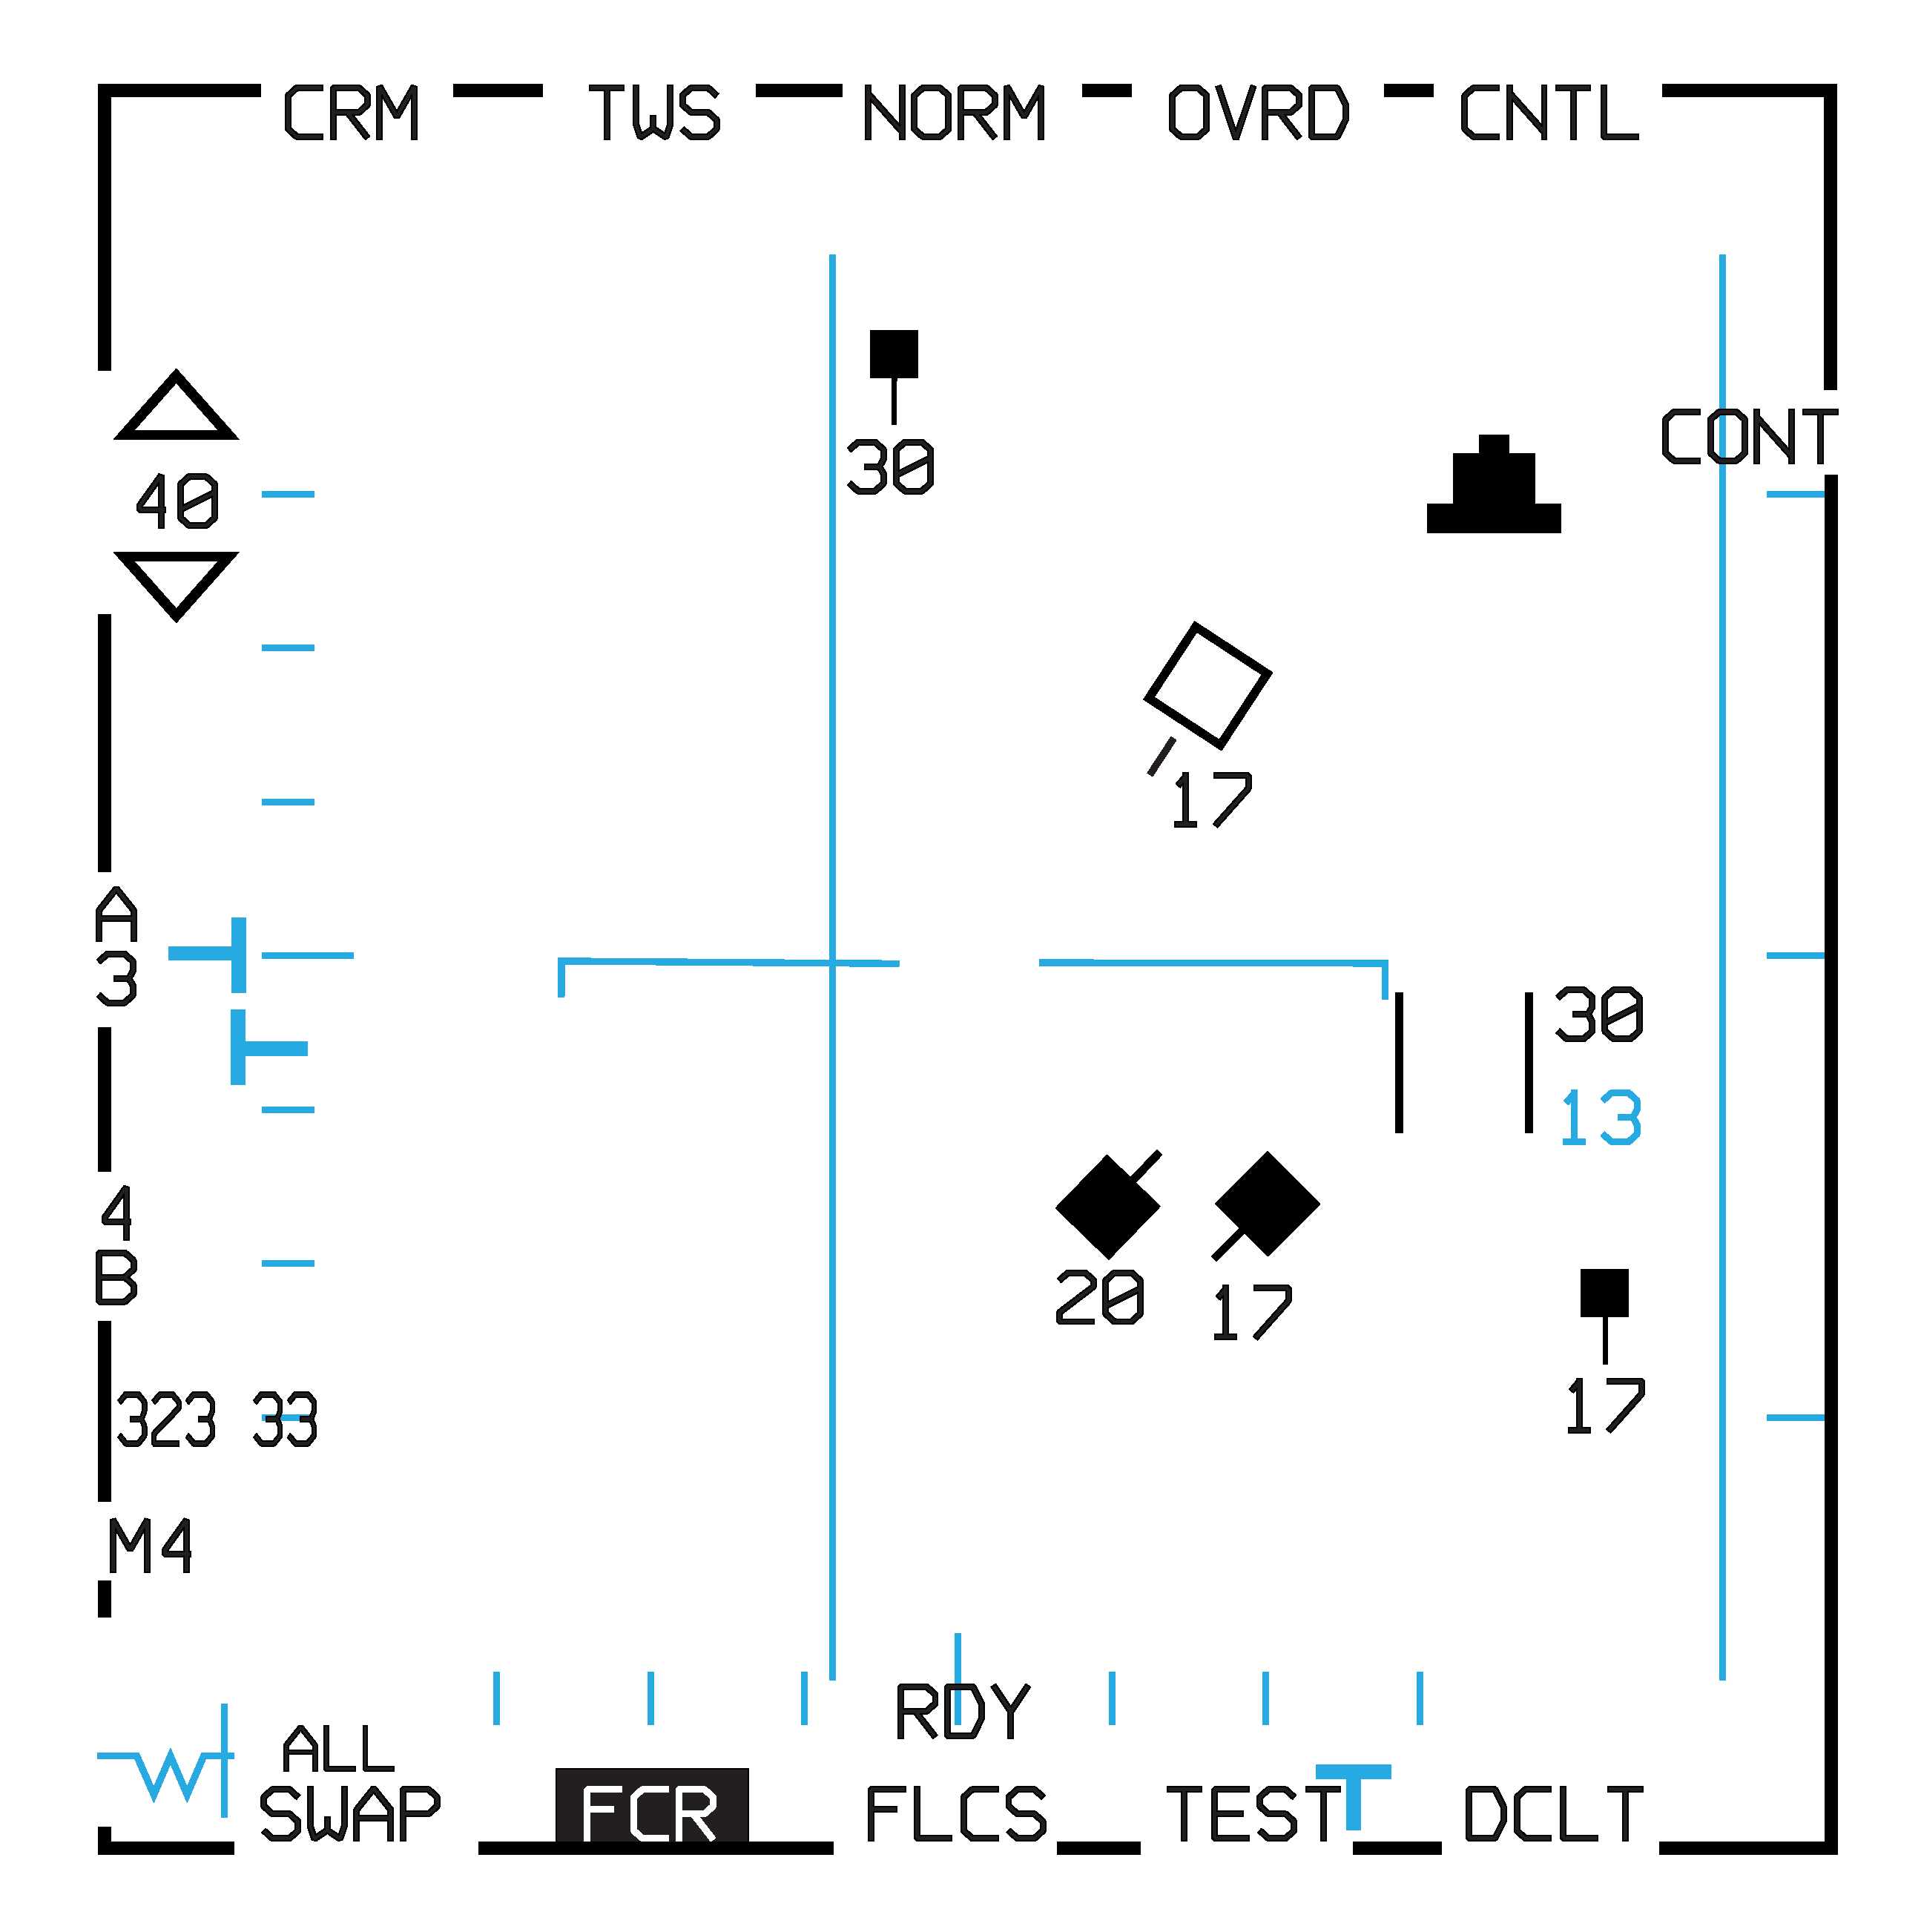
\includegraphics[
                height=75mm,
            ]{mfd/fcr_aa/tws_search.pdf}
        };

        % Annotations
        \node[lannot] (search) at ($(fig.west)+(0mm,28mm)$) {Search target};
        \draw[annotptr] (search.east) -- ++(30mm, 0mm) -- ++(4mm, -4mm);

        \node[lannot] (sec) at ($(fig.west)+(0mm,8mm)$) {Azimuth scan limits};
        \draw[annotptr] (sec.east) -- ++(32mm, 0mm);

        \node[rannot] (as) at ($(fig.east)+(0mm,24mm)$) {Current STPT};
        \draw[annotptr] (as.west) -- ++(-12mm, 0mm) -- ++(-3mm, -3mm);

        \node[rannot] (system) at ($(fig.east)+(0mm,10mm)$) {System \\ target};
        \draw[annotptr] (system.west) -- ++(-26mm, 0mm);

        \node[rannot] (cursor) at ($(fig.east)+(0mm,-4mm)$) {Acquisition cursor};
        \draw[annotptr] (cursor.west) -- ++(-11mm, 0mm);

        \node[rannot] (searchr) at ($(fig.east)+(0mm,-15mm)$) {Search \\ target};
        \draw[annotptr] (searchr.west) -- ++(-11mm, 0mm);

        \node[rannot] (asec) at ($(fig.east)+(0mm,-26mm)$) {Track \\ targets};
        \draw[annotptr] (asec.west) -- ++(-20mm, 0mm) -- ++(-6mm,10mm);
    \end{tikzpicture}
    \caption{Basic TWS search FCR page symbology.}
    \label{fig:sensors_aa:apg68:tws:search}
\end{figure}

\begin{figure}[htbp]
    \centering
    \begin{subfigure}[b]{0.15\linewidth}
        \centering
        
\includegraphics[
            scale=0.75,
        ]{mfd/fcr_aa/tgt_search.pdf}
        \caption{Search}
        \label{fig:sensorsaa:apg68:tws:trackfile:search}
    \end{subfigure}
    \begin{subfigure}[b]{0.15\linewidth}
        \centering
        
\includegraphics[
            scale=0.75,
        ]{mfd/fcr_aa/tgt_track.pdf}
        \caption{Track}
        \label{fig:sensorsaa:apg68:tws:trackfile:track}
    \end{subfigure}
    \begin{subfigure}[b]{0.15\linewidth}
        \centering
        
\includegraphics[
            scale=0.75,
        ]{mfd/fcr_aa/tgt_system.pdf}
        \caption{System}
        \label{fig:sensorsaa:apg68:tws:trackfile:system}
    \end{subfigure}
    \begin{subfigure}[b]{0.15\linewidth}
        \centering
        
\includegraphics[
            scale=0.75,
        ]{mfd/fcr_aa/tgt_cursor.pdf}
        \caption{Cursor}
        \label{fig:sensorsaa:apg68:tws:trackfile:cursor}
    \end{subfigure}
    \begin{subfigure}[b]{0.15\linewidth}
        \centering
        
\includegraphics[
            scale=0.75,
        ]{mfd/fcr_aa/tgt_bugged.pdf}
        \caption{Bugged}
        \label{fig:sensorsaa:apg68:tws:trackfile:bugged}
    \end{subfigure}
    \caption{TWS Track Symbols}
    \label{fig:sensorsaa:apg68:tws:trackfile}
\end{figure}

\subsubsection{TRACKFILE STATES}
\label{subsec:sensorsaa:apg68:tws:trackfile}
\begin{tcoloritemize}
    \blueitem[Search Target]

    \textbf{Initial state for radar returns}
    \begin{itemize}
        \item not enough information to generate track
        \item automatic transition to track after 1-2 radar sweeps
        \item \textbf{Display} --- similar to RWS radar brick
    \end{itemize}

    Reference \cref{fig:sensorsaa:apg68:tws:trackfile:search}
    \blueitem[Track Target]
    
    \textbf{FCR automatically correlates radar return data to form track files}
    \begin{itemize}
    \item tracks target velocity, angle, altitude etc.
    \item \textbf{\underline{maximum of 10 trackfiles}}, lowest priority dropped if exceeded
    \item can be manually transitioned to higher modes by pilot to prioritize
    \end{itemize}

    Reference \cref{fig:sensorsaa:apg68:tws:trackfile:track}
    \blueitem[System Target]
    
    \textbf{Allows pilot to designate targets of interest}
    \begin{itemize}
        \item for monitoring
        \item for future weapons employment
        \item \textbf{no additional radar energy allocated to System Targets}
    \end{itemize}

    Reference \cref{fig:sensorsaa:apg68:tws:trackfile:system}
    \blueitem[Cursor Target]
        
    \textbf{Acquisition Cursor ``snaps'' to nearby System Targets} --- therefore named Cursor Targets
    \begin{itemize}
        \item \textbf{scan centered on Cursor Target}
        \begin{itemize}
            \item 3 bar elevation
            \item $\pm$25 deg azimuth pattern 
            \item reduces chance of losing track
        \end{itemize}
    \end{itemize}

    Reference \cref{fig:sensorsaa:apg68:tws:trackfile:cursor,fig:sensorsaa:apg68:tws:cursorsymb}
    \blueitem[Bugged Target]
        
    \textbf{Selected for weapons employment}
    \begin{itemize}
        \item can guide AIM-120C (w/o STT Lock)
        \item DLZ displayed if missile selected
        \item launched AIM-120 will continue to guide even if another target is bugged --- \textbf{\underline{allows for multi-target engagement}} 
        \item \textbf{scan Centered on Bugged Target}
        \begin{itemize}
            \item 3 bar elevation
            \item $\pm$25 deg azimuth pattern 
            \item reduces chance of losing track
        \end{itemize}
        \item \textbf{TMS Right --- Cycles through System Targets in range order} (bugs closest if none bugged)
    \end{itemize}

    Reference \cref{fig:sensorsaa:apg68:tws:trackfile:bugged,fig:sensorsaa:apg68:tws:buggedsymb}
    \blueitem[Spotlight] \textbf{Narrow scan centered on acquisition cursor}
    \begin{itemize}
        \item \textbf{narrow scan}
        \begin{itemize}
            \item 4 bar elevation 
            \item \pm10 deg azimuth
        \end{itemize}
        \item allows pilot to override TWS scan priority
        \item \textbf{activated by holding TMS Forward >1 sec}
    \end{itemize}
\end{tcoloritemize}

\begin{figure}[htbp]
    \centering
    \begin{tikzpicture}[auto, node distance=10mm, x=1mm, y=1mm, very thick, line cap=round,
        >={Latex[round]}
        ]
        
        \node[] (mfd) at (0,0) {
            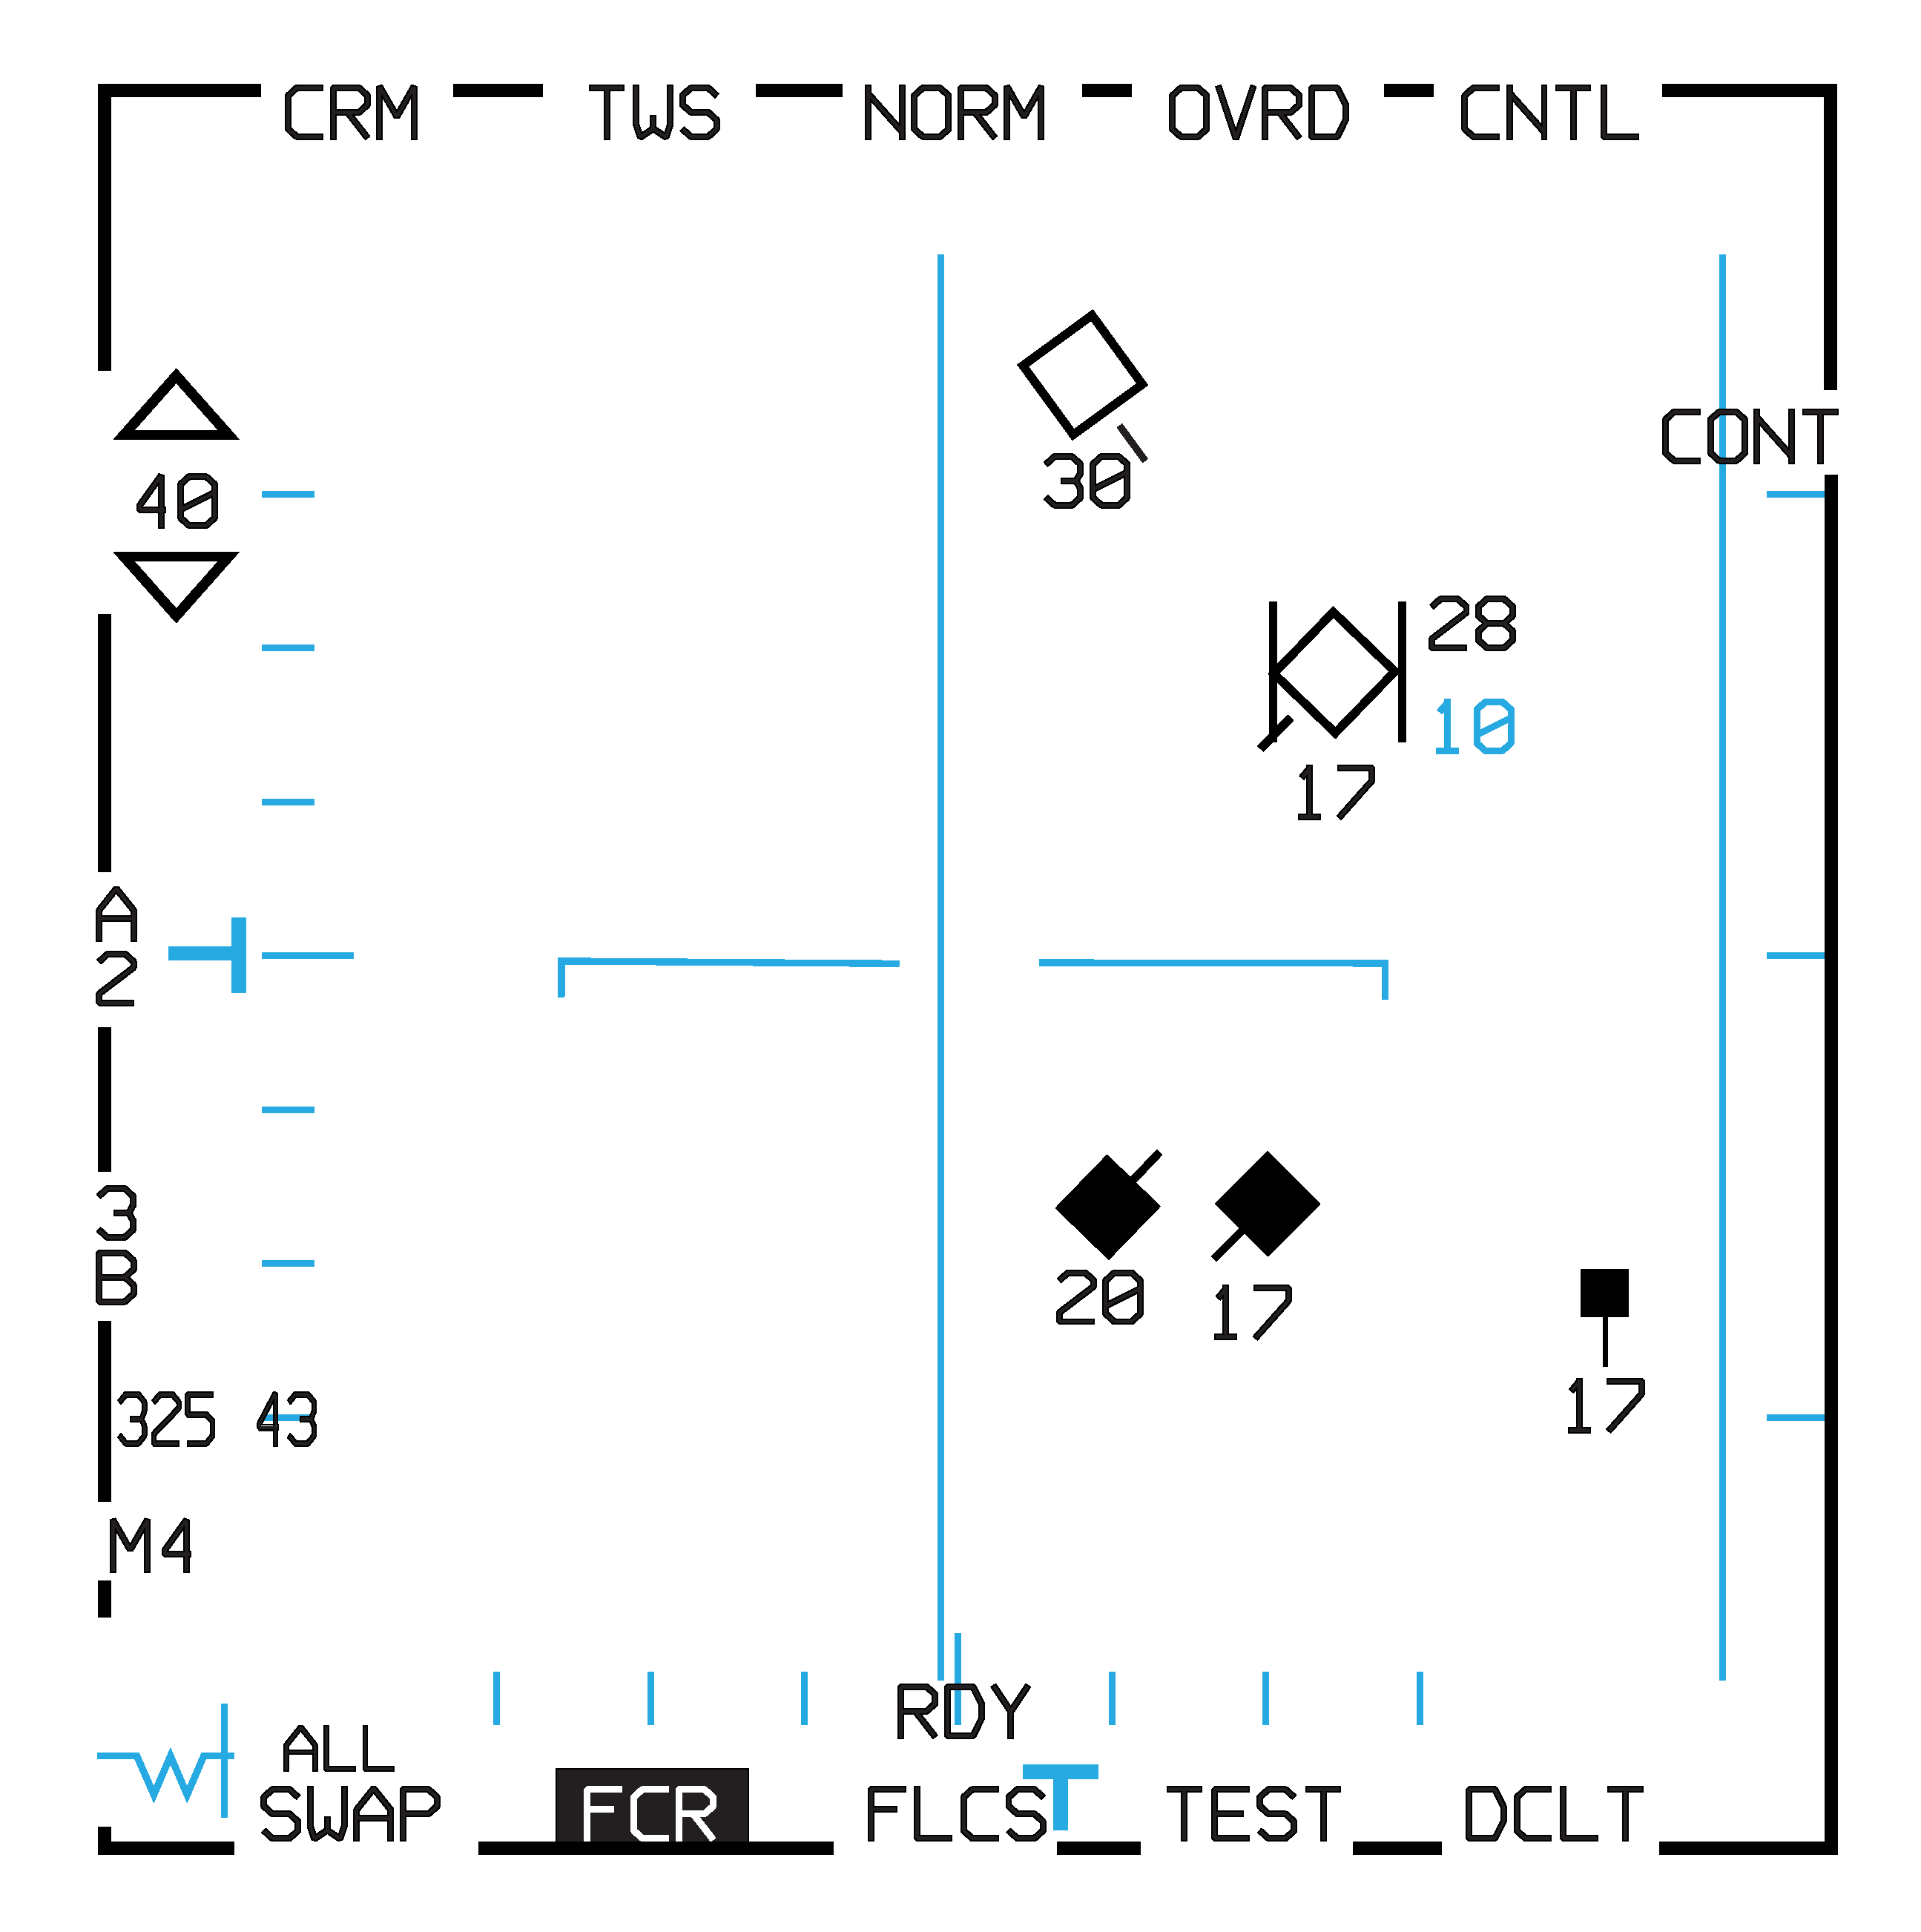
\includegraphics[
                height=75mm,
            ]{mfd/fcr_aa/tws_cursor.pdf}
        };

        % Annotations
        \node[lannot] (system) at ($(fig.west)+(0mm,29mm)$) {System \\ target};
        \draw[annotptr] (system.east) -- ++(37mm, 0mm) -- ++(4mm, -4mm);

        \node[lannot] (sec) at ($(fig.west)+(0mm,8mm)$) {Azimuth scan limits};
        \draw[annotptr] (sec.east) -- ++(36mm, 0mm);

        \node[rannot] (cursor) at ($(fig.east)+(0mm,11mm)$) {Cursor \\ target};
        \draw[annotptr] (cursor.west) -- ++(-15mm, 0mm);

        \node[rannot] (searchr) at ($(fig.east)+(0mm,-15mm)$) {Search \\ target};
        \draw[annotptr] (searchr.west) -- ++(-11mm, 0mm);

        \node[rannot] (asec) at ($(fig.east)+(0mm,-26mm)$) {Track \\ targets};
        \draw[annotptr] (asec.west) -- ++(-20mm, 0mm) -- ++(-6mm,10mm);
    \end{tikzpicture}
    \caption{TWS FCR page symbology with cursor target}
    \label{fig:sensorsaa:apg68:tws:cursorsymb}
\end{figure}

\begin{figure}[htbp]
    \centering
    \begin{tikzpicture}[auto, node distance=10mm, x=1mm, y=1mm, very thick, line cap=round,
        >={Latex[round]}
        ]
        
        \node[] (mfd) at (0,0) {
            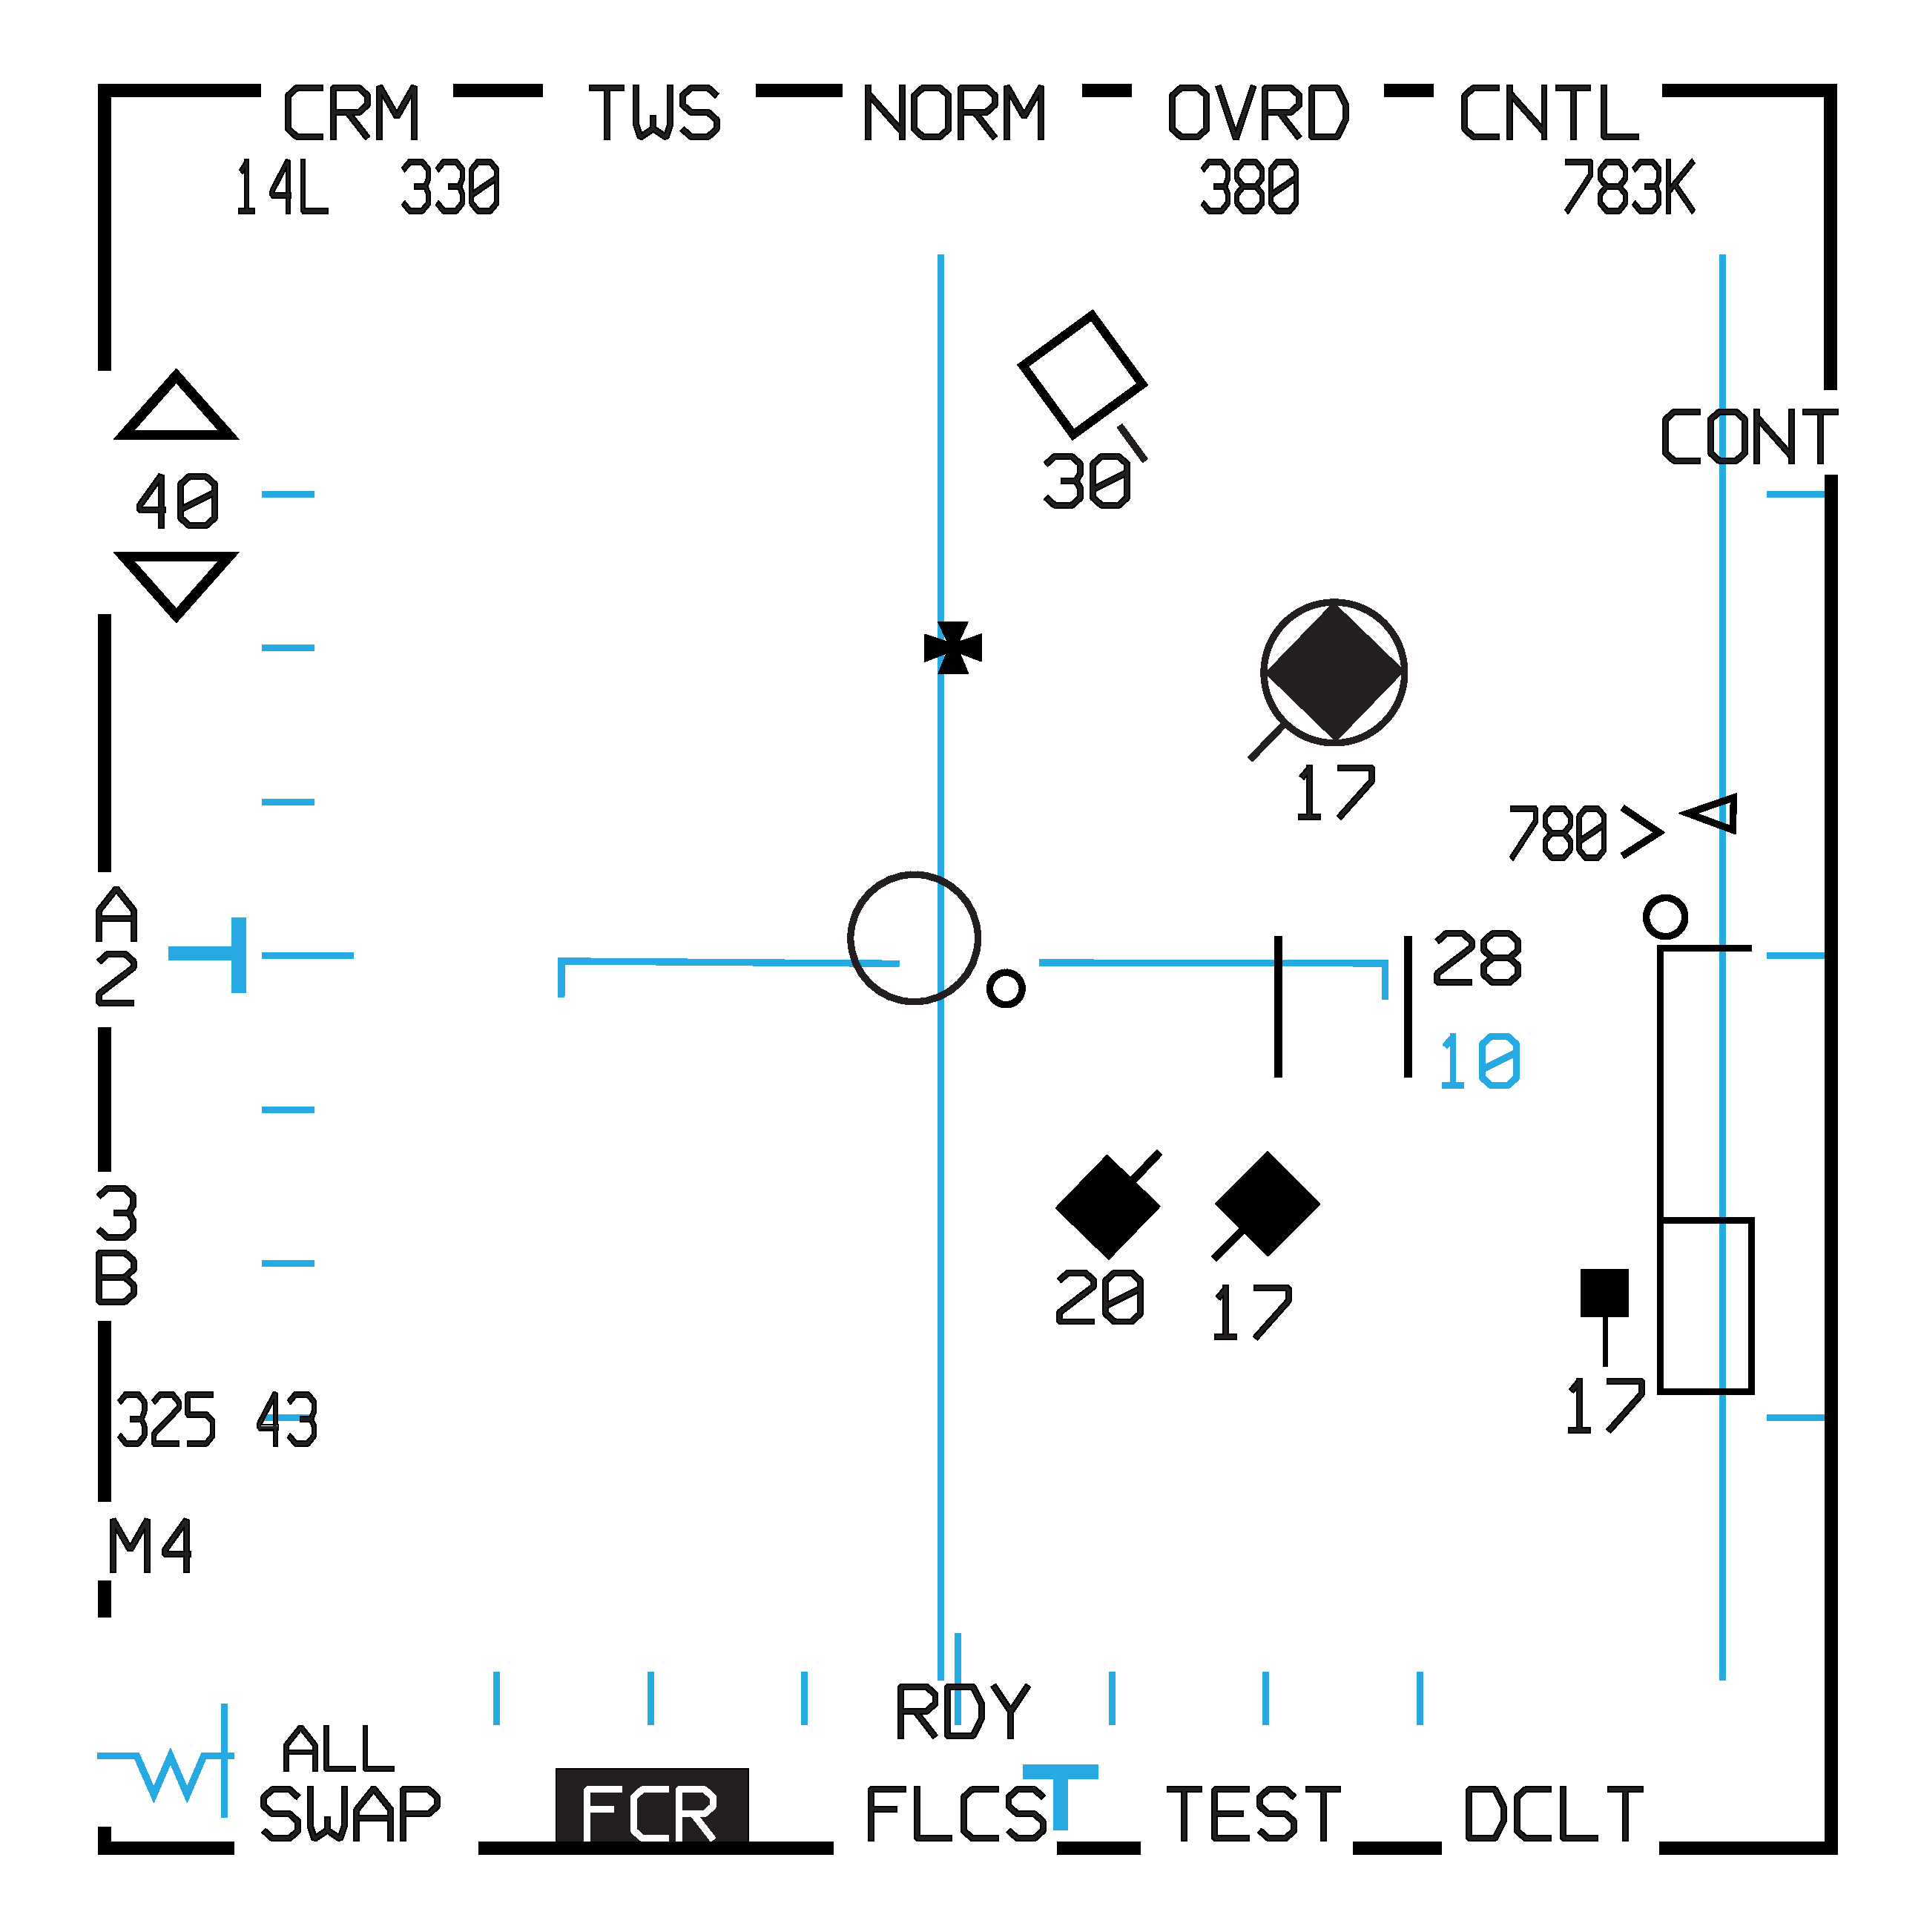
\includegraphics[
                height=75mm,
            ]{mfd/fcr_aa/tws_bugged.pdf}
        };

        % Annotations
        \node[lannot] (asp) at ($(fig.west)+(0mm,30.25mm)$) {Aspect};
        \draw[annotptr] (asp.east) -- ++(9mm, 0mm);

        \node[lannot] (trk) at ($(fig.west)+(0mm,24mm)$) {Track};
        \draw[annotptr] (trk.east) -- ++(12mm, 0mm) -- ++(4mm, 4mm);

        % \node[lannot] (system) at ($(fig.west)+(0mm,15mm)$) {System \\ target};
        % \draw[annotptr] (system.east) -- ++(37mm, 0mm) -- ++(4mm, 4mm);

        \node[lannot] (cross) at ($(fig.west)+(0mm,7mm)$) {Steering \\ cross};
        \draw[annotptr] (cross.east) -- ++(32mm, 0mm) -- ++(4mm, 4mm);

        % \node[lannot] (sec) at ($(fig.west)+(0mm,-8mm)$) {Azimuth scan limits};
        % \draw[annotptr] (sec.east) -- ++(36mm, 0mm);

        \node[lannot] (asec) at ($(fig.west)+(0mm,-6mm)$) {ASC / ASEC \\ {\footnotesize see \cref{fig:aa_weap:aim120:asc_asec}}};
        \draw[annotptr] (asec.east) -- ++(30mm, 0mm) -- ++(4mm, 4mm);

        \node[rannot] (clos) at ($(fig.east)+(0mm,30.25mm)$) {Closure};
        \draw[annotptr] (clos.west) -- ++(-9mm, 0mm);

        \node[rannot] (as) at ($(fig.east)+(0mm,24mm)$) {Airspeed};
        \draw[annotptr] (as.west) -- ++(-22mm, 0mm) -- ++(-4mm, 4mm);

        \node[rannot] (bug) at ($(fig.east)+(0mm,11mm)$) {Bugged \\ target};
        \draw[annotptr] (bug.west) -- ++(-20mm, 0mm);

        \node[rannot] (dlz) at ($(fig.east)+(0mm,-10mm)$) {DLZ \\ {\footnotesize see \cref{fig:aa_weap:aim120:dlz}}};
        \draw[annotptr] (dlz.west) -- ++(-7mm, 0mm);

        \node[rannot] (asec) at ($(fig.east)+(0mm,-26mm)$) {Track \\ targets};
        \draw[annotptr] (asec.west) -- ++(-20mm, 0mm) -- ++(-6mm,10mm);
    \end{tikzpicture}
    \caption{
        TWS FCR page symbology with bugged target. 
        Note that ``shoot'' symbology (DLZ, ASEC, steering cross) 
        as well as additional information about the bugged target is displayed.
    }
    \label{fig:sensorsaa:apg68:tws:buggedsymb}
\end{figure}

\marginfigeometry

\subsubsection{SELECT TWS MODE}
\begin{checklistenumerate}
    \blueitem[FCR Switch] \textbf{FCR}
    \blueitem[Desired MFD] \textbf{FCR Page}, verify \textbf{SOI}
    \blueitem[Radar Mode]
    \textbf{CRM} (default), verify

    \begin{itemize}
        \item \textbf{Dogfight/Missile Override} --- \textbf{NORM}
        \item \textbf{Radar Mode (OSB 1)} --- shows \textbf{CRM}
    \end{itemize}
    \blueitem[CRM Submode]
    \textbf{TWS}, cycle via 

    \begin{itemize}
        \item \textbf{TMS Right (long)} / \textbf{OSB 2} 
    \end{itemize}
\end{checklistenumerate}

\subsubsection{MULTI-TARGET ACQUISITION}
\label{subsec:tws:multiacq}
\begin{checklistenumerate}
    \blueitem[Track Target Acquisition]
    \label{subsec:sensorsaa:apg68:tws:multi:trk}
    \marginpar{
        \captionsetup{type=figure}
        \centering
        \begin{tikzpicture}[figstyle]
            
            \node[
                boxedmarfigstyle,            
            ] (search) at (0,0) {
                
\includegraphics[
                    scale=0.5,
                ]{mfd/fcr_aa/tgt_search.pdf}
            };
            \node[
                boxedmarfigstyle,               
                below=10 of search,
            ] (track) {
                
\includegraphics[
                    scale=0.5,
                ]{mfd/fcr_aa/tgt_track.pdf}
            };
            \node[
                boxedmarfigstyle,
                below=17.5 of track,
            ] (system) {
                
\includegraphics[
                    scale=0.5,
                ]{mfd/fcr_aa/tgt_system.pdf}
            };
            \node[
                boxedmarfigstyle,                
                below=12.5 of system,
            ] (cursor) {
                
\includegraphics[
                    scale=0.5,
                ]{mfd/fcr_aa/tgt_cursor.pdf}
            };
            \node[
                boxedmarfigstyle,                
                below=10 of cursor,
            ] (bugged) {
                
\includegraphics[
                    scale=0.5,
                ]{mfd/fcr_aa/tgt_bugged.pdf}
            };

            % lines
            \draw[->]
            (search) -- node[right, align=left, font=\small] {\textbf{Automatic}}(track);
            \path (search) -- node[left, align=right, font=\small] {\ref{subsec:sensorsaa:apg68:tws:multi:trk}}(track);
            \draw[->]
            (track) -- node[right, align=left, font=\small] {\textbf{TMS FWD} \\ \footnotesize\textbf{(repeat for all} \\ \footnotesize\textbf{desired targets)}}(system);
            \draw[>-]
            ($(track.south)!0.5!(system.north) + (-5,0)$) -- ++(0,2) arc (180:0:2.5) -- ++(0,-4) arc (360:180:2.5) -- node[left, align=right, font=\small, pos=1] {\ref{subsec:sensorsaa:apg68:tws:multi:sys}} ++(0,2);
            \draw[->]
            (system) -- node[right, align=left, font=\small] {\textbf{Slew Cursor} \\ \textbf{near target}}(cursor);
            \draw[->]
            (cursor) -- node[right, align=left, font=\small] {\textbf{TMS FWD}}(bugged);
            \path (cursor) -- node[left, align=right, font=\small] {\ref{subsec:sensorsaa:apg68:tws:multi:bug}}(bugged);

            % labels
            \node[
                anchor=north west,
                align=left,
                font=\bfseries\footnotesize,
            ] (labelsearch) at (search.north west) {Search \\ Target};
            \node[
                anchor=north west,
                align=left,
                font=\bfseries\footnotesize,
            ] (labeltrack) at (track.north west) {Track \\ Target};
            \node[
                anchor=north west,
                align=left,
                font=\bfseries\footnotesize,
            ] (labelsystem) at (system.north west) {System \\ Target};
            \node[
                anchor=north west,
                align=left,
                font=\bfseries\footnotesize,
            ] (labelcursor) at (cursor.north west) {Cursor \\ Target};
            \node[
                anchor=north west,
                align=left,
                font=\bfseries\footnotesize,
            ] (labelbugged) at (bugged.north west) {Bugged \\ Target};
        \end{tikzpicture}
        \caption{TWS trackfile acquisition flow}
    }
    \begin{enumerate}
        \item Correlate onboard/offboard sensors to locate targets
        \begin{itemize}
            \item raw radar returns, RWR pings
            \item AWACS calls, datalink targets
        \end{itemize}
        \item Place targets within radar scan volume
        \item FCR automatically generates Track Targets once sufficient data available
    \end{enumerate}
    \blueitem[System Target Acquisition]
    \label{subsec:sensorsaa:apg68:tws:multi:sys}
    \begin{enumerate}
        \item \textbf{Target} \dotfill under Acquisition Cursor
        \item \textbf{TMS} \dotfill \textbf{Forward} 
    \end{enumerate}
    Repeat for all desired Track Targets,
    or to upgrade all Track Targets:
    \begin{enumerate}
        \item \textbf{TMS} \dotfill \textbf{Right}
    \end{enumerate}
    \blueitem[Upgrade to Bugged Target]
    \label{subsec:sensorsaa:apg68:tws:multi:bug}
    \begin{enumerate}
        \item \textbf{Target} \dotfill under Acquisition Cursor
        \item \textbf{TMS} \dotfill \textbf{Forward}
    \end{enumerate}
    To select closest System Target 
    \begin{enumerate}
        \item \textbf{TMS} \dotfill \textbf{Right}
    \end{enumerate}
    To cycle through System Targets in range order
    \begin{enumerate}
        \item \textbf{TMS} \dotfill \textbf{Right}
    \end{enumerate}
    \blueitem[STT Lock] (if desired)
    \begin{enumerate}
        \item \textbf{Bugged Target} \dotfill under Acq Cursor
        \item \textbf{TMS} \dotfill \textbf{Forward}
    \end{enumerate}
\end{checklistenumerate}

\marginfigrestore

\subsection{ACM}
\label{subsec:acm}
\begin{tcoloritemize}
    \blueitem{ACM}{
    \textbf{A}ir \textbf{C}ombat \textbf{M}ode

    \begin{subitemize}
        \item \textbf{Used to automatically lock targets while maneuvering}
        \item \textbf{Sub-Modes}
        \begin{itemize}
            \item \textbf{HUD Scan} --- 30x20 deg 
            \item \textbf{BORE} --- Boresight (3x3 deg)
            \item \textbf{Vertical Scan} --- 10x60 deg
            \item \textbf{Slewable} --- WIP
        \end{itemize}
    \end{subitemize}}
\end{tcoloritemize}

\begin{figure}[htbp]
    \centering
    \begin{tikzpicture}[auto, node distance=10mm, x=1mm, y=1mm, very thick,
        >={Latex[round]}
        ]
        
        % \node[<options>](<coordinate name>)at(<coordinate>){<text>};
        \node[
            hyperref node=subsec:acm,
            rectangle,
            rounded corners,
            minimum width=15mm,
            minimum height=15mm,
            draw,
        ](acm)at(0,0){\blue{ACM}};
        \node[
            rectangle,
            rounded corners,
            minimum width=20mm,
            minimum height=7.5mm,
            draw,
        ](bore)at(0,20){\textbf{BORE}};
        \node[
            rectangle,
            rounded corners,
            minimum width=20mm,
            minimum height=7.5mm,
            draw,
        ](hud)at(32.5,0){\textbf{HUD}};
        \node[
            rectangle,
            rounded corners,
            minimum width=20mm,
            minimum height=7.5mm,
            draw,
        ](vert)at(0,-20){\textbf{Vertical}};
        \node[
            hyperref node=subsec:stt,
            rectangle, 
            rounded corners,
            minimum width=90mm,
            minimum height=7.5mm,
            draw, 
        ](stt)at(0,35){\blue{STT}};
                
        % Lines
        \draw [->]
            (acm) -- node[pos=0.5, left]{\scriptsize\textbf{TMS FWD}} (bore);
        \draw [->]
            (acm) -- node[pos=0.5, above]{\scriptsize\textbf{TMS}}node[pos=0.5, below]{\scriptsize\textbf{RIGHT}} (hud);
        \draw [->]
            (acm) -- node[pos=0.5, left]{\scriptsize\textbf{TMS AFT}} (vert);
        \draw [->]
            let
                \p1=(bore.north),
                \p2=(stt.south),
            in
                (\p1) -- node[pos=0.5, left]{\scriptsize\textbf{Automatic}} (\x1,\y2);
        \draw [->]
            let
                \p1=(hud.north),
                \p2=(stt.south),
            in
                (\p1) -- node[pos=0.5, left]{\scriptsize\textbf{Automatic}} (\x1,\y2);
        \draw [->, rounded corners]
            let
                \p1=(vert.west),
                \p2=(stt.south),
            in
                (\p1) -- (\x1-22.5mm,\y1) -- node[pos=0.5, left]{\scriptsize\textbf{Automatic}} (\x1-22.5mm,\y2);
                
    \end{tikzpicture}
    \caption{ACM Radar Modes Overview}
    \label{fig:acmoverview}
\end{figure}

\begin{figure}[htbp]
    \centering
    \begin{tikzpicture}[auto, node distance=10mm, x=1mm, y=1mm, very thick, line cap=round,
        >={Latex[round]}
        ]
        
        \node[] (fig) at (0,0) {
            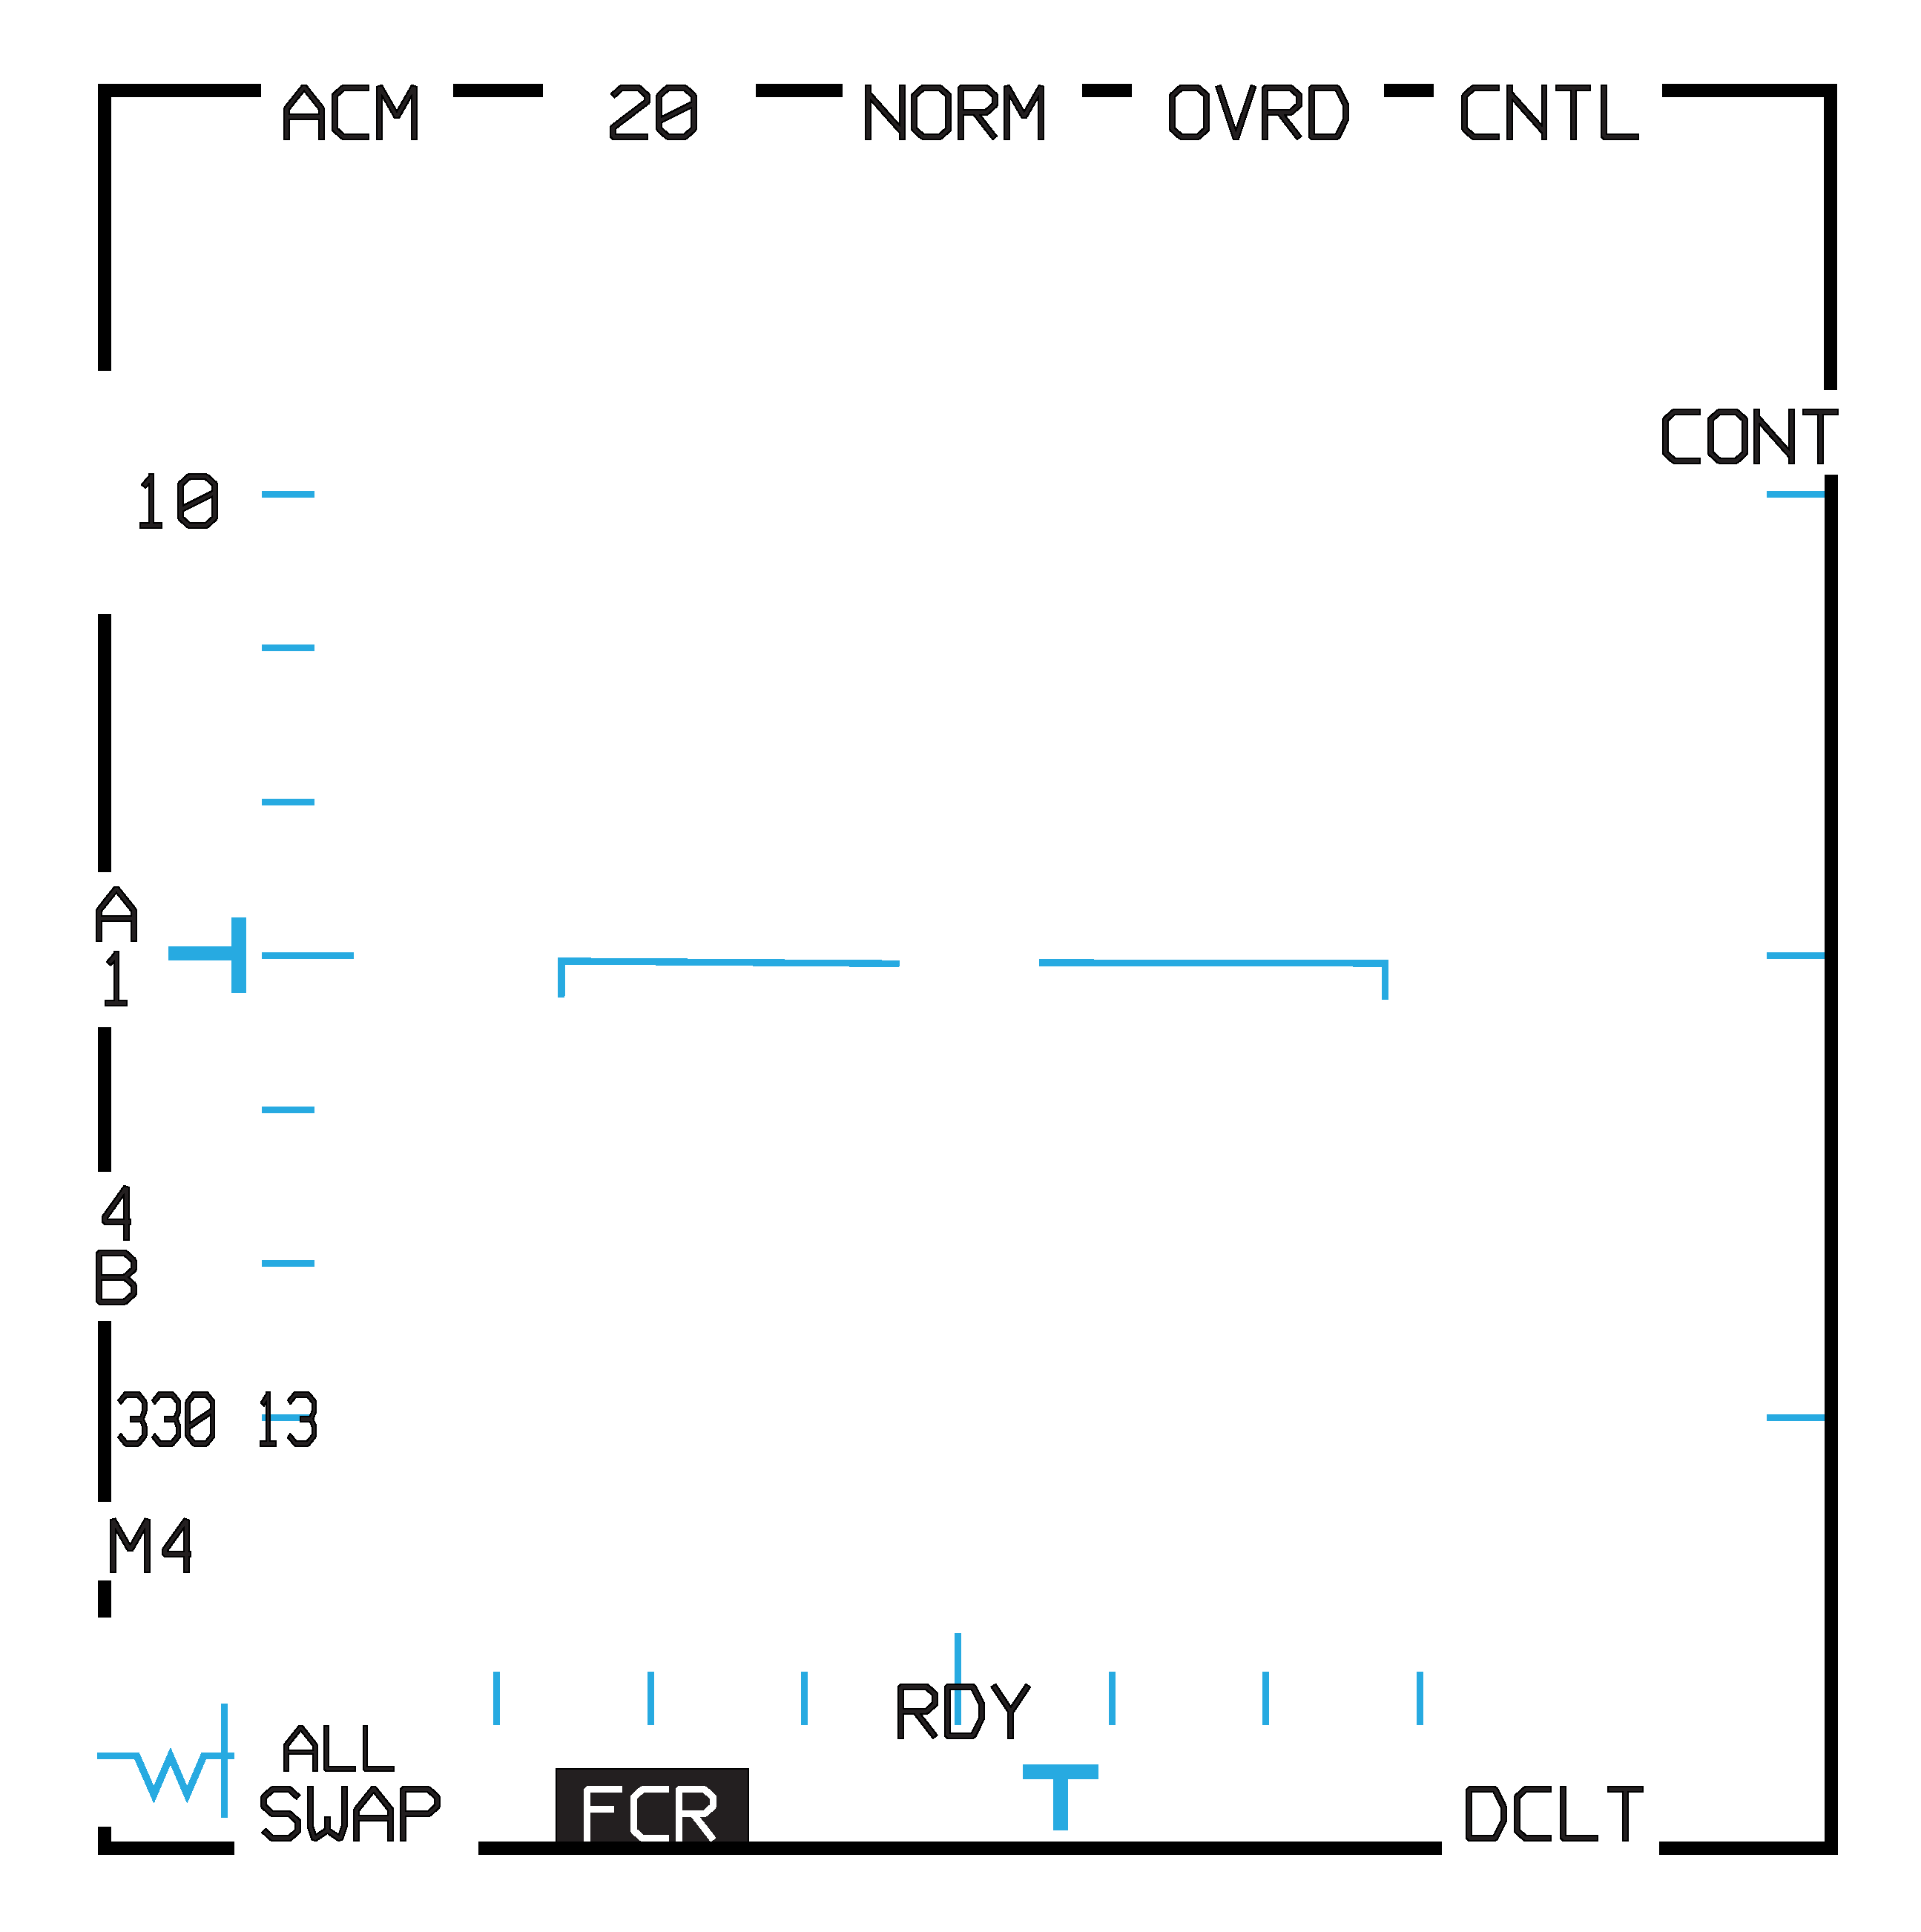
\includegraphics[
                height=75mm,
            ]{mfd/fcr_aa/acm_homepage.pdf}
        };

        % Annotations
        \node[lannot] (mode) at ($(fig.west)+(0mm,38mm)$) {FCR mode};
        \draw[->, red] (mode.east) -- ++(12mm, 0mm) -- (-24mm,35mm);

        \node[lannot] (submode) at ($(fig.west)+(0mm,28mm)$) {ACM \\ submode};
        \draw[->, red] (submode.east) -- ++(23mm, 0mm) -- (-13mm, 31mm);

        \node[lannot] (rsel) at ($(fig.west)+(0mm,18mm)$) {Range scale};
        \draw[->, red] (rsel.east) -- ++(4.5mm, 0mm);

        \node[lannot] (asel) at ($(fig.west)+(0mm,0.5mm)$) {Azimuth};
        \draw[->, red] (asel.east) -- ++(4.5mm, 0mm);

        \node[lannot] (bsel) at ($(fig.west)+(0mm,-10.5mm)$) {Elevation \\ bar};
        \draw[->, red] (bsel.east) -- ++(4.5mm, 0mm);

        \node[annot, anchor=south, align=center] (fov) at ($(fig.north)+(0mm,0mm)$) {FOV select};
        \draw[->, red] (fov.south) -- ++(0mm, -3.5mm);

        \node[rannot] (cntl) at ($(fig.east)+(0mm,38mm)$) {Control};
        \draw[->, red] (cntl.west) -- ++(-13mm, 0mm) -- (23mm, 35mm);

        \node[rannot] (ovrd) at ($(fig.east)+(0mm,28mm)$) {Override};
        \draw[->, red] (ovrd.west) -- ++(-24mm, 0mm) -- (12mm, 31mm);

        \node[rannot] (dl) at ($(fig.east)+(0mm,20.5mm)$) {Datalink mode};
        \draw[->, red] (dl.west) -- ++(-4mm,0mm);

        \node[rannot] (sj) at ($(fig.east)+(0mm,-8mm)$) {Horizon \\indicator};
        \draw[->, red] (sj.west) -- ++(-20mm, 0mm) -- (12mm,-1mm);

        \node[rannot] (dclt) at ($(fig.east)+(0mm,-38mm)$) {Declutter};
        \draw[->, red] (dclt.west) -- ++(-13mm, 0mm) -- (23mm, -35mm);
    \end{tikzpicture}
    \caption{ACM FCR page symbology}
\end{figure}

\begin{figure}[htbp]
    \centering
    \begin{subfigure}[t]{0.3\linewidth}
        \centering
        \begin{tikzpicture}[figstyle]
            
            \draw[color2, fill=color2!20, dashed, rounded corners]
            (-15, 10) -- (15,10) -- (15,-10) -- (-15,-10) -- cycle;

            \node[] (fig) at (0,0) {
                
\includegraphics[
                    scale=0.25,
                ]{hud/acm/subfig_hud.pdf}
            };

        \end{tikzpicture}
        \caption{HUD}
    \end{subfigure}
    \begin{subfigure}[t]{0.3\linewidth}
        \centering
        \begin{tikzpicture}[figstyle]

            \draw[color2, fill=color2!20, dashed] 
            (0,-3) circle [x radius=4, y radius=6];
            
            \node[] (bore) at (0,0) {
                
\includegraphics[
                    scale=0.25,
                ]{hud/acm/subfig_bore.pdf}
            };
    
        \end{tikzpicture}
        \caption{BORE}
    \end{subfigure}
    \begin{subfigure}[t]{0.3\linewidth}
        \centering
        \begin{tikzpicture}[figstyle]

            \draw[color2, fill=color2!20, dashed, rounded corners]
            (-2.5, 30) -- (2.5,30) -- (2.5,-8) -- (-2.5,-8) -- cycle;
            
            \node[] (vert) at (0,0) {
                \includegraphics[
                    scale=0.25,
                ]{hud/acm/subfig_vert.pdf}
            };
    
        \end{tikzpicture}
        \caption{Vertical}
    \end{subfigure}
    \caption{
        ACM Scan Patterns shown with the relevant HUD symbology. 
        The dashed lines indicate the scan volume for illustrative purposes and are not to scale.
    }
\end{figure}

\begin{figure}[htbp]
    \centering
    \begin{tikzpicture}[auto, node distance=10mm, x=1mm, y=1mm, very thick, line cap=round,
        >={Latex[round]}
        ]

        \node[draw, rounded corners] (fig) at (0,0) {
            \includegraphics[
                height=75mm,
            ]{hud/acm/bore.pdf}
        };

        % Annotations
        \node[lannot] (bs) at ($(fig.west)+(-2.5mm,34mm)$) {Boresight cross};
        \draw[->, red] (bs.east) -- ++(34mm,0mm) -- ++(4mm,-4mm);

        \node[lannot] (eegs) at ($(fig.west)+(-2.5mm,24mm)$) {EEGS funnel};
        \draw[->, red] (eegs.east) -- ++(32mm,0mm);

        \node[lannot] (acc) at ($(fig.west)+(-2.5mm,13.5mm)$) {Acceleration};
        \draw[->, red] (acc.east) -- ++(16mm,0mm);

        \node[lannot] (cas) at ($(fig.west)+(-2.5mm,0mm)$) {Airspeed \\ {\footnotesize calibrated}};
        \draw[->, red] (cas.east) -- ++(7mm,0mm);

        \node[lannot] (dgft) at ($(fig.west)+(-2.5mm,-15mm)$) {Mode};
        \draw[->, red] (dgft.east) -- ++(9mm,0mm) -- ++(4mm, -4mm);

        \node[lannot] (mgrs) at ($(fig.west)+(-2.5mm,-32mm)$) {MGRS lines};
        \draw[->, red] (mgrs.east) -- ++(10mm,0mm);

        \node[rannot] (bore) at ($(fig.east)+(2.5mm,13mm)$) {Scan zone indicator};
        \draw[->, red] (bore.west) -- ++(-38mm, 0mm);

        \node[rannot] (alt) at ($(fig.east)+(2.5mm,0mm)$) {Altimeter};
        \draw[->, red] (alt.west) -- ++(-12mm, 0mm);

        \node[rannot] (arc) at ($(fig.east)+(2.5mm,-12mm)$) {Attitude arc};
        \draw[->, red] (arc.west) -- ++(-28mm, 0mm);

        \node[rannot] (slant) at ($(fig.east)+(2.5mm,-25.25mm)$) {Target slant range};
        \draw[->, red] (slant.west) -- ++(-20mm, 0mm);
    \end{tikzpicture}
    \caption{ACM HUD Symbology. Shown in BORE submode.}
\end{figure}

\begin{figure}[htbp]
    \centering
    \begin{tikzpicture}[auto, node distance=10mm, x=1mm, y=1mm, very thick, line cap=round,
        >={Latex[round]}
        ]

        \node[draw, rounded corners] (fig) at (0,0) {
            \includegraphics[
                height=60mm,
            ]{hmd/dgft.pdf}
        };

        % Annotations
        \node[lannot] (rwr) at ($(fig.west)+(-2.5mm,22.5mm)$) {RWR};
        \draw[->, red] (rwr.east) -- ++(7mm,0mm);

        \node[lannot] (acc) at ($(fig.west)+(-2.5mm,16.5mm)$) {Acceleration};
        \draw[->, red] (acc.east) -- ++(8mm,0mm) -- ++(4mm, -2mm);

        \node[lannot] (cas) at ($(fig.west)+(-2.5mm,9.5mm)$) {Airspeed};
        \draw[->, red] (cas.east) -- ++(5.5mm,0mm);

        \node[lannot] (cross) at ($(fig.west)+(-2.5mm,2mm)$) {Aiming cross};
        \draw[->, red] (cross.east) -- ++(28mm,0mm) -- ++(5mm,5mm);

        \node[lannot] (dgft) at ($(fig.west)+(-2.5mm,-6.5mm)$) {Mode};
        \draw[->, red] (dgft.east) -- ++(7mm,0mm);

        \node[lannot] (hdg) at ($(fig.west)+(-2.5mm,-26mm)$) {Heading \\ {\footnotesize HMD LOS}};
        \draw[->, red] (hdg.east) -- ++(22mm,0mm);

        \node[rannot] (acq) at ($(fig.east)+(2.5mm,22.5mm)$) {Acquisition circle};
        \draw[->, red] (acq.west) -- ++(-28mm,0mm) -- ++(-4mm,-4mm);

        \node[rannot] (alt) at ($(fig.east)+(2.5mm,9.5mm)$) {Altimeter};
        \draw[->, red] (alt.west) -- ++(-6mm, 0mm);

        \node[rannot] (range) at ($(fig.east)+(2.5mm,-1mm)$) {Target slant range};
        \draw[->, red] (range.west) -- ++(-10mm, 0mm) -- ++(-4mm, -4mm);

        \node[rannot] (stpt) at ($(fig.east)+(2.5mm,-14.5mm)$) {Distance to STPT};
        \draw[->, red] (stpt.west) -- ++(-8mm, 0mm);
    \end{tikzpicture}
    \caption{
        ACM HMD Symbology. 
        Shown in BORE submode. 
        Note that RWR indication is of highest threat 
        with diamond indicating direction of threat 
        and gap indicating current HMD LOS.
    }
\end{figure}

\begin{tcoloritemize}
    \blueitem{HUD Submode}{
    \begin{subitemize}
        \item \textbf{30x20 deg scan} --- slightly larger than HUD
        \item \textbf{Lock Range} --- 10 nm
        \item \textbf{Selected with TMS Right} --- default mode upon ACM selection
        \item \textbf{Default ACM mode} --- but in \textbf{NO RAD} (non-radiating) state
        \item \textbf{Displays}
        \begin{itemize}
            \item \textbf{FCR Format} --- displays \textbf{ACM 20}
            \item \textbf{HUD} --- no special symbology
        \end{itemize}
    \end{subitemize}}
    \blueitem{BORE Submode}{
    \begin{subitemize}
        \item \textbf{Small, 1-beamwidth scan}
        \begin{itemize}
            \item centered 3 deg below gun cross
            \item useful for precisely locking up target
        \end{itemize}
        \item \textbf{Lock Range} --- 20 nm
        \item \textbf{Selected with TMS Forward}
        \item \textbf{Scan slaves to HMD} (if equipped and powered)
        \item \textbf{Displays}
        \begin{itemize}
            \item \textbf{FCR Format} --- displays \textbf{ACM BORE}
            \item \textbf{HUD} --- Boresight Cross at center of radar scan zone
            \item \textbf{HMD} --- Oval centered on HMD aiming cross
        \end{itemize}
    \end{subitemize}}
    \blueitem{Vertical \break Submode}{
    \begin{subitemize}
        \item \textbf{10x60 deg scan}
        \begin{itemize}
            \item centered 23 deg above gun cross
            \item useful during turning engagement to lock target ``across the circle''
        \end{itemize}
        \item \textbf{Lock Range} --- 10 nm
        \item \textbf{Selected with TMS Aft}
        \item \textbf{Displays}
        \begin{itemize}
            \item \textbf{FCR Format} --- displays \textbf{ACM 60}
            \item \textbf{HUD} --- Vertical line
        \end{itemize}
    \end{subitemize}}
    \blueitem{Slewable \break Submode --- WIP}{
    \begin{subitemize}
        \item \textbf{Scan} --- WIP
        \item \textbf{Lock Range} --- WIP
        \item \textbf{Slew} --- \textbf{CURSOR/ENABLE Control}
        \item \textbf{Displays}
        \begin{itemize}
            \item \textbf{FCR Format} --- displays \textbf{ACM SLEW}
            \item \textbf{HUD} --- WIP
        \end{itemize}
    \end{subitemize}}
    \blueitem{NO RAD}{Upon selection of \textbf{ACM} or dropping target lock the radar is placed in non-radiating state}
\end{tcoloritemize}

\marginfigeometry

\subsubsection{HUD / BORE / VERTICAL ACQUISITION}
\begin{checklistenumerate}
    \blueitem{FCR Setup}{
    \marginpar{
        \captionsetup{type=figure}
        \begin{subfigure}[t]{\linewidth}
            \centering
            \begin{tikzpicture}[auto, node distance=10mm, x=1mm, y=1mm, very thick, line cap=round,
                >={Latex[round]}
                ]
    
                \draw[color2, fill=color2!20, dashed, rounded corners]
                (-15, 10) -- (15,10) -- (15,-10) -- (-15,-10) -- cycle;
                
                \node[] (hud) at (0,0) {
                    \includegraphics[
                        scale=0.25,
                    ]{hud/acm/subfig_hud.pdf}
                };
        
            \end{tikzpicture}
            \caption{HUD}
        \end{subfigure}
        \begin{subfigure}[t]{0.45\linewidth}
            \centering
            \begin{tikzpicture}[auto, node distance=10mm, x=1mm, y=1mm, very thick, line cap=round,
                >={Latex[round]}
                ]
    
                \draw[color2, fill=color2!20, dashed] 
                (0,-3) circle [x radius=4, y radius=6];
                
                \node[] (bore) at (0,0) {
                    \includegraphics[
                        scale=0.25,
                    ]{hud/acm/subfig_bore.pdf}
                };
        
            \end{tikzpicture}
            \caption{BORE}
        \end{subfigure}
        \begin{subfigure}[t]{0.45\linewidth}
            \centering
            \begin{tikzpicture}[auto, node distance=10mm, x=1mm, y=1mm, very thick, line cap=round,
                >={Latex[round]}
                ]
    
                \draw[color2, fill=color2!20, dashed, rounded corners]
                (-2.5, 30) -- (2.5,30) -- (2.5,-8) -- (-2.5,-8) -- cycle;
                
                \node[] (vert) at (0,0) {
                    \includegraphics[
                        scale=0.25,
                    ]{hud/acm/subfig_vert.pdf}
                };
        
            \end{tikzpicture}
            \caption{Vertical}
        \end{subfigure}
        \caption{HUD / BORE / VERTICAL Symbology}
    }
    \begin{subenumerate}
        \item \textbf{FCR Switch} \dotfill \textbf{FCR}
        \item \textbf{Desired MFD} \dotfill \textbf{FCR Page}
    \end{subenumerate}}
    \blueitem{Enter ACM}{
    \begin{subenumerate}
        \item \textbf{Dogfight/Missile Override} \dotfill \textbf{DGFT}
        \item \textbf{Radar Mode (OSB 2)} \dotfill verify \textbf{ACM}
    \end{subenumerate}}
    \blueitem{Select ACM Submode}{
    \begin{subitemize}
        \item \textbf{HUD} (default ACM mode) \dotfill \textbf{TMS Right}
        \item \textbf{Bore} \dotfill \textbf{TMS Forward}
        \item \textbf{Vertical} \dotfill \textbf{TMS Aft}
    \end{subitemize}}
    \blueitem{Target Acquisition}{
    \begin{subenumerate}
        \item Maneuver aircraft to place target within selected ACM scan volume 
        \item Wait for automatic transition to STT 
    \end{subenumerate}}
    \blueitem{Target Rejection}{%
    To unlock target
    \begin{subenumerate}
        \item \textbf{TMS} \dotfill \textbf{Aft}
    \end{subenumerate}
    Radar returns to \textbf{HUD} submode in \textbf{NO RAD} 
    }
\end{checklistenumerate}

\subsubsection{HMD ACQUISITION}
\begin{checklistenumerate}
    \blueitem{FCR/MFD Setup}{
    \marginpar{
        \captionsetup{type=figure}
        \centering
        \includegraphics[
            height=25mm,
        ]{hmd/dgft_subfig_bore.pdf}
        \caption{HMD acquisition circle}
    }
    \begin{subenumerate}
        \item \textbf{FCR Switch} \dotfill \textbf{FCR}
        \item \textbf{Desired MFD} \dotfill \textbf{FCR Page}
        \item \textbf{HMD Brightness} \dotfill \textbf{On}
    \end{subenumerate}}
    \blueitem{Enter ACM}{
    \begin{subenumerate}
        \item \textbf{Dogfight/Missile Override} \dotfill \textbf{DGFT}
        \item \textbf{Radar Mode (OSB 2)} \dotfill verify \textbf{ACM}
    \end{subenumerate}}
    \blueitem{Select ACM Bore Submode}{
    \begin{subitemize}
        \item \textbf{Bore} \dotfill \textbf{TMS Forward}
    \end{subitemize}}
    \blueitem{Target Acquisition}{
    \begin{subenumerate}
        \item Maneuver aircraft to place target within 60 deg of nose 
        \item Place target within HMD acquisition circle
        \item Wait for automatic transition to STT 
    \end{subenumerate}}
    \blueitem{Target Rejection}{%
    To unlock target
    \begin{subenumerate}
        \item \textbf{TMS} \dotfill \textbf{Aft}
    \end{subenumerate}
    Radar returns to \textbf{HUD} submode in \textbf{NO RAD} 
    }
\end{checklistenumerate}

\subsubsection{SLEWABLE ACQUISITION --- WIP}

\marginfigrestore

\subsection{STT}
\label{subsec:stt}
\begin{tcoloritemize}
    \blueitem{STT}{
    \textbf{S}ingle \textbf{T}arget \textbf{T}rack
    \begin{subitemize}
        \item \textbf{FCR continually scans one target}
        \begin{itemize}
            \item high update frequency \& precision for weapon guidance
            \item \underline{target RWR will detect STT lock}
        \end{itemize}
        \item \textbf{FCR search ceases during STT lock}
        \item \textbf{Entered by}
        \begin{itemize}
            \item locking bugged target from \textbf{TWS/RWS} with \textbf{TMS Forward}
            \item placing target in search volume of \textbf{ACM} (lock occurs automatically)
        \end{itemize}
        \item \textbf{Exited with TMS Aft} --- returns to search mode
    \end{subitemize}}
    \blueitem{Display}{
    \begin{subitemize}
        \item \textbf{Target state} shown at top of FCR page
        \begin{itemize}
            \item aspect angle 
            \item ground track 
            \item airspeed 
            \item closure rate
        \end{itemize}
    \end{subitemize}}
    \blueitem{NCTR}{
    \textbf{N}on-\textbf{C}ooperative \textbf{T}arget \textbf{R}ecognition
    \begin{subitemize}
        \item \textbf{FCR attempts to identify locked target}
        \begin{itemize}
            \item measures turbine parameters to produce \underline{likely} contact aircraft type
            \item NCTR is only available in STT
        \end{itemize}
        \item \textbf{NCTR imposes additional requirements}
        \begin{itemize}
            \item target must be within 20-25nm
            \item radar must ``see'' compressor/turbine blades
        \end{itemize}
        \item \textbf{Activated with IFF interrogation (TMS Left long)}
        \item \textbf{Hostile NCTR identification counts towards ROE matrix} (combined with IFF return)
    \end{subitemize}}
\end{tcoloritemize}

\begin{figure}[htbp]
    \centering
    \begin{tikzpicture}[auto, node distance=10mm, x=1mm, y=1mm, very thick, line cap=round,
        >={Latex[round]}
        ]
        
        \node[] (mfd) at (0,0) {
            \includegraphics[
                height=100mm,
                page={37},
            ]{F16_apg68_RWS_HomePage&SAM_v6-1.pdf}
        };

        \node[] at (0,-20) {\color{red}\textbf{MISSING ANNOTATIONS}};
    \end{tikzpicture}
    % \fbox{
    % \begin{minipage}[t][75mm][t]{100mm}
    %     \center{\large\textbf{MFD --- FCR --- STT}}
    %     \begin{itemize}
    %         \item Show standard STT lock
    %         \item should clearly mark target state, steering cues, dlz, NCTR
    %     \end{itemize}
    % \end{minipage}
    % }
    \caption{FCR page with STT lock and NCTR ID}
\end{figure}


\clearpage 

\section{IFF --- WIP}
\label{sec:iff}

\begin{tcoloritemize}
    \blueitem{IFF}{
    \textbf{I}dentify \textbf{F}riend or \textbf{F}oe
    \begin{itemize}
        \item \textbf{Unknown contacts can be ``interrogated'' to determine if friendly}
        \item \textbf{Works via transponder system}
        \begin{itemize}
            \item Interrogater sends coded pulse
            \item Friendly transponder return matching coded pulse
        \end{itemize}
        \item \textbf{Controlled via dedicated IFF panel}
        \begin{itemize}
            \item Must be powered on separately from FCR to function
        \end{itemize}
        \item \textbf{Friendly IFF replies displayed as green circles on FCR MFD}
    \end{itemize}}
    \blueitem{Manual \break Interrogation}{
    Manual IFF interrogation can be initiated in 2 modes

    \begin{itemize}
        \item \textbf{Scan} --- Interrogates entire radar scan volume
        \begin{itemize}
            \item Activated by pressing \textbf{TMS Left (short)}
            \item \textbf{SCAN} appears next to \textbf{OSB 16} on FCR page
        \end{itemize}
        \item \textbf{LOS} (\textbf{L}ine \textbf{O}f \textbf{S}ight) --- Interrogates locked target or scan volume around acquisition cursor
        \begin{itemize}
            \item Actived by pressing \textbf{TMS Left (long)}
            \item \textbf{LOS} appears next to \textbf{OSB 16} on FCR page
        \end{itemize}
    \end{itemize}}
\end{tcoloritemize}

\warningbox{
    \textbf{Lack of IFF return does \underline{not} necessarily mean target is hostile} 
    \begin{itemize}
        \item system relies on active participation of interrogated target
        \item depending on ROE, additional information may be required prior to weapon employment
    \end{itemize}
}

\notebox{
    \textbf{IFF has independent transponder, can function even when FCR is not radiating}
}

% \subsubsection{IFF DED PAGE}

% \begin{figure}[htbp]
%     \centering
%     \fbox{
%     \begin{minipage}[t][30mm][t]{100mm}
%         \center{\large\textbf{IFF DED Display}}
%         \begin{itemize}
%             \item Standard DED display (with IFF information bottom left)
%         \end{itemize}
%     \end{minipage}
%     }
%     \caption{DED IFF Status}
% \end{figure}

% \subsubsection{INTG DED PAGE}

% \subsubsection{IFF CONTROL PANEL}

% \begin{figure}[htbp]
%     \centering
%     \fbox{
%     \begin{minipage}[t][75mm][t]{100mm}
%         \center{\large\textbf{IFF Panel}}
%         \begin{itemize}
%             \item Show IFF panel (\underline{just} IFF panel)
%         \end{itemize}
%     \end{minipage}
%     }
%     \caption{IFF Control Panel}
% \end{figure}


% \begin{tcoloritemize}
%     \blueitem{Master Switch}{
%     Controls operating mode of IFF system when \textbf{C\&I Switch} is set to \textbf{BACKUP}

%     \begin{itemize}
%         \item \textbf{OFF} --- removes power from system
%         \item \textbf{STBY} --- system is powered but in standby mode
%         \item \textbf{NORM} --- normal operating mode
%     \end{itemize}
%     }
%     \blueitem{M-4 Code Switch}{}
%     \blueitem{C \& I Switch}{
%     Selects source for \textbf{C}ommunications \textbf{\&} \textbf{I}FF control

%     \begin{itemize}
%         \item \textbf{BACKUP}
%         \begin{itemize}
%             \item \textbf{UHF} and \textbf{IFF} panels used to control relevant systems
%             \item Can be activated without system fault
%         \end{itemize}
%         \item \textbf{UFC} --- \textbf{U}p \textbf{F}ront \textbf{C}ontrols
%         \begin{itemize}
%             \item Sets input source as UFC (ICP \& DED) for both IFF and UHF
%         \end{itemize}
%     \end{itemize}}
%     \blueitem{Enable Switch}{}
%     \blueitem{Mode 1 / 3 Selectors}{}
%     \blueitem{Mode 4 Reply Switch}{}
%     \blueitem{Mode 4 Monitor Switch}{}
% \end{tcoloritemize}

\marginfigeometry

\subsection{INTERROGATION}
\label{sec:iff:interrogation}
\begin{checklistenumerate}
    \blueitem{Prerequisites}{
    % \marginpar{
    %     \captionsetup{type=figure}
    %     \fbox{
    %         \begin{minipage}[t][40mm][t]{\marginparwidth}
    %             \center{\textbf{IFF Control Panel Location}}
    %             \begin{itemize}[leftmargin=1em]
    %                 \item show panel location like in start up
    %             \end{itemize}
    %         \end{minipage}
    %     }
    %     \caption{IFF Control Panel}
    % }
    % TODO: add iff figures!
    \begin{itemize}
        \item \textbf{C\&I Switch} \dotfill \textbf{UFC}
        \item \textbf{IFF Master Mode Switch} \dotfill \textbf{NORM}
        \item \textbf{Desired MFD} \dotfill \textbf{FCR Page}, \textbf{SOI}
    \end{itemize}
    
    Not necessary, but highly recommended
    
    \begin{itemize}
        \item \textbf{FCR Switch} \dotfill \textbf{FCR}
    \end{itemize}}
    \blueitem{Locate Targets}{
    \begin{enumerate}
        \item Correlate onboard/offboard sensors
        \begin{itemize}
            \item raw radar returns, RWR pings
            \item AWACS calls, datalink targets
        \end{itemize}
        \item Place target within radar scan volume
    \end{enumerate}}
    \blueitem{Interrogate}{
    % \marginpar{
    %     \captionsetup{type=figure}
    %     \fbox{
    %         \begin{minipage}[t][80mm][t]{\marginparwidth}
    %             \center{\textbf{IFF Return Symbology}}
    %             \begin{itemize}[leftmargin=1em]
    %                 \item show symbology elements for IFF returns (friendly and non friendly)
    %             \end{itemize}
    %         \end{minipage}
    %     }
    %     \caption{IFF Symbology}
    % }
    % TODO: add me!

    \smallskip
    To interrogate the entire radar scan volume

    \begin{enumerate}
        \item \textbf{TMS} \dotfill \textbf{Left (short)}
    \end{enumerate}

    To interrogate the currently locked target or volume around the cursor 

    \begin{enumerate}
        \item \textbf{TMS} \dotfill \textbf{Left (long)}
    \end{enumerate}}
    \blueitem{Evaluate Returns}{After 1-3 sec IFF replies should appear

    \begin{itemize}
        \item Friendlies are marked by green circles
        \item Depending on avionics and radar mode, radar tracks may be marked in green to indicate friendly
    \end{itemize}}
\end{checklistenumerate}

\marginfigrestore

\clearpage

\section{DATALINK --- WIP}

\cleardoublepage
	\cyclechpcolor
	\chapter[A-G SENSORS --- WIP]{A-G SENSORS}
\thumbtab{A-G Sensors}{4}
\localtableofcontents
\thispagestyle{plain}
\cleardoublepage

% \section{APG-68 FCR}
% \label{sec:fcr-ag}

% \subsection{GM}

% \subsection{GMT}

% \section{LITENING TGP}

% \clearpage 

% \section{HARM TARGETING SYSTEM}

% \cleardoublepage
	\part{Weapons}
	\cyclechpcolor
	\part{Weapons}

\chapter{A-G WEAPONS --- WIP}
\thumbtab{A-G}{4}
\localtableofcontents
\cleardoublepage

% \section{SELECTIVE JETTISON}

% \clearpage

% \section{M-61 CANNON}

% \clearpage 

% \section{UNGUIDED ORDNANCE}

% \subsection{MARK 80-SERIES}
% \subsection{ROCKETS}
% \subsection{CBU-87}
% \subsection{CBU-97}
% \subsection{BDU-33 - TRAINING BOMB}
% \subsection{BDU-50LD/HD - TRAINING BOMB}

% \clearpage 

% \section{LASER-GUIDED ORDNANCE}

% \subsection{GBU-10/12 - PAVEWAY II}
% \subsection{GBU-24 - PAVEWAY III}
% \subsection{BDU-50LGB - TRAINING LGB}

% \clearpage 

% \section{GPS-GUIDED ORDNANCE}
% \subsection{JDAM}
% \subsection{JSOW}
% \subsection{CBU-103/105 - WCMD}

% \clearpage

% \section{AGM-65 MAVERICK}

% \clearpage 

% \section{AGM-88C HARM}

% \subsection{ALIC TABLES}
% \subsection{HAS MODE}
% \subsection{POS MODE}

% \cleardoublepage
	\cyclechpcolor
	\chapter{A-A WEAPONS}
\thumbtab{A-A}{6}
\localtableofcontents
\thispagestyle{plain}
\cleardoublepage

\section{AIR-TO-AIR GUNNERY}

\subsection{M-61 VULCAN}
\label{subsec:m61}

\begin{figure}[htbp]
    \centering
    \fbox{
    \begin{minipage}[t][40mm][t]{100mm}
        \center{\large\textbf{M-61 OVERVIEW}}
        \begin{itemize}
            \item Some kind of overview figure
            \item maybe showing side on profile of the weapon?
        \end{itemize}
    \end{minipage}
    }
    \caption{M-61 Vulcan}
\end{figure}

\begin{tcoloritemize}
    \blueitem{M-61 Vulcan}{
    Internally mounted, high fire-rate, 20mm rotary ``Gattling'' cannon.
    In service since 1959

    \begin{subitemize}
        \item \textbf{Fire Rate} --- 6000rpm
        \item \textbf{Round Size} --- 20mm
        \item \textbf{Ammo Capacity} --- 510 rounds
    \end{subitemize}}
    \blueitem{Ammunition Types}{
    \begin{subitemize}
        \item \textbf{HEI} --- \textbf{H}igh \textbf{E}xplosive \textbf{I}ncendiary
        \item \textbf{HEI-T} --- \textbf{H}igh \textbf{E}xplosive \textbf{I}ncendiary-\textbf{T}racer
        \item \textbf{AP} --- \textbf{A}rmor \textbf{P}iercing
        \item \textbf{TP} --- \textbf{T}arget \textbf{P}ractice
        \item \textbf{SAPHEI} --- \textbf{S}emi \textbf{A}rmor \textbf{P}iercing \textbf{H}igh \textbf{E}xplosive \textbf{I}ncendiary
    \end{subitemize}}
    \blueitem{Gunsight / \break Cueing Modes}{
    \begin{subitemize}
        \item \textbf{EEGS} --- \textbf{E}nhanced \textbf{E}nvelope \textbf{G}un\textbf{S}ight \\
        \hyperref[subsec:m61:eegssymb]{See \Cref{subsec:m61:eegssymb}}
        \item \textbf{Employment w/o radar track (EEGS level II)} \\
        \hyperref[subsec:m61:eegslvl2]{See \Cref{subsec:m61:eegslvl2}}
        \item \textbf{Employment with radar track (EEGS level V)} \\
        \hyperref[subsec:m61:eegslvl5]{See \Cref{subsec:m61:eegslvl5}}
    \end{subitemize}}
    \blueitem{Select GUN}{
    Via Dogfight --- AIM-9 \& GUN automatically selected

    \begin{subenumerate}
        \item \textbf{DGFT/MSL OVRD} \dotfill \textbf{DGFT}
    \end{subenumerate}

    Via A-A Master Mode

    \begin{subenumerate}
        \item \textbf{Master Mode} \dotfill \textbf{A-A}
        \item \textbf{SMS OSB 1} \dotfill \textbf{Cycle to GUN}
    \end{subenumerate}}
\end{tcoloritemize}

\subsubsection{SMS CONTROLS}
\label{subsec:m61:sms}
\begin{tcoloritemize}
    \blueitem{Operating Mode}{\textbf{OSB 1} cycles A-A modes, should display \textbf{GUN}}
    \blueitem{Sub-Mode}{\textbf{OSB 2} cycles gunsight modes
    
    \begin{subitemize}
        \item \textbf{EEGS} --- \textbf{E}nhanced \textbf{E}nvelope \textbf{G}un\textbf{S}ight \\
        \textbf{See \Cref{subsec:m61:eegssymb}}
    \end{subitemize}}
    \blueitem{Rounds \break Remaining}{Indicates number of rounds remaining in 10s}
\end{tcoloritemize}

\begin{figure}[htbp]
    \centering
    \begin{tikzpicture}[auto, node distance=10mm, x=1mm, y=1mm, very thick, line cap=round,
        >={Latex[round]}
        ]
        
        \node[] (fig) at (0,0) {
            \includegraphics[
                height=75mm,
                page={79},
            ]{weap_aa_v11.pdf}
        };

        % Annotations
        \node[lannot] (mode) at ($(fig.west)+(0mm,27mm)$) {Operating \\ mode};
        \draw[->, red] (mode.east) -- ++(10mm, 0mm) -- (-25mm,29mm);

        \node[lannot] (submode) at ($(fig.west)+(0mm,14mm)$) {Submode};
        \draw[->, red] (submode.east) -- ++(22.5mm, 0mm) -- (-11mm, 29mm);

        \node[rannot] (inv) at ($(fig.east)+(0mm,27mm)$) {Inventory};
        \draw[->, red] (inv.west) -- ++(-21mm, 0mm) -- (14mm, 29mm);

        \node[rannot] (rounds) at ($(fig.east)+(0mm,14mm)$) {Rounds \\ remaining};
        \draw[->, red] (rounds.west) -- ++(-8mm,0mm) -- (28mm, 18mm);

        \node[rannot] (rdy) at ($(fig.east)+(0mm,0mm)$) {Ready \\ indication};
        \draw[->, red] (rdy.west) -- ++(-20mm, 0mm) -- (10mm,18mm);

        \node[rannot] (sj) at ($(fig.east)+(0mm,-14mm)$) {Selective Jettison};
        \draw[->, red] (sj.west) -- ++(-12.5mm, 0mm) -- ($(fig.south) + (22mm,12mm)$);
    \end{tikzpicture}
    \caption{Gun SMS page}
\end{figure}

\subsubsection{EEGS SYMBOLOGY}
\label{subsec:m61:eegssymb}
\begin{tcoloritemize}
    \blueitem{EEGS}{\textbf{E}nhanced \textbf{E}nvelope \textbf{G}un\textbf{S}ight

    \begin{subitemize}
        \item \textbf{Provides multiple levels of symbology depending on presence of radar lock}
    \end{subitemize}}
    \blueitem{Level I}{Backup mode displaying only boresight cross in event of INS failure}
    \blueitem{Level II}{Operating mode prior to radar lock

    \begin{subitemize}
        \item \textbf{Boresight Cross} --- shows where gun / aircraft is pointed
        \item \textbf{EEGS Funnel}
        \begin{itemize}
            \item displays path of rounds through space
            \item funnel is of set width to judge distance --- adjust width to target wingspan, stabilize edges of funnel on wingtips and fire
        \end{itemize}
        \item \textbf{MGRS} --- \textbf{M}ultiple \textbf{R}eference \textbf{G}un\textbf{S}ight
        \begin{itemize}
            \item 5 line-segments pointing towards boresight
            \item reference for high aspect snap shots (placeing target on MGRS line should have it fly through gun cross)
        \end{itemize}
    \end{subitemize}
    
    Reference symbology in \cref{fig:aa_weap:m61:eegslvl2}
    }
    \blueitem{Level III / IV}{Intermediate modes during radar lock acquisition}
    \blueitem{Level V}{Operating mode with radar lock. Level II symbology is retained with additional elements
    
    \begin{subitemize}
        \item \textbf{Level V Pipper}
        \begin{itemize}
            \item gunfire solution --- stabilize pipper on target and fire
            \item contains additional range/aspect cues
        \end{itemize}
        \textbf{reference \cref{fig:aa_weap:m61:eegslvl5,fig:aa_weap:m61:eegs:5pipper}}
        \item \textbf{T-Symbol}
        \begin{itemize}
            \item \textbf{``--- + ---'' 1G Pipper} --- lead angle for non-maneuvering target,
            flanking horizontal lines indicate out-of-plane maneuver potential of target
            \item \textbf{``---'' Max-G Pipper} --- lead angle for target pulling max-G towards you
        \end{itemize}
        \textbf{reference \cref{fig:aa_weap:m61:eegs:tsymb}}
        \item \textbf{Range Caret}
        \begin{itemize}
            \item displayed on \underline{inside} edge of level V pipper
            \item unwinds from 12 o'clock at 12'000ft counter-clockwise
        \end{itemize}
        \textbf{reference \cref{fig:aa_weap:m61:eegs:tdescirc}}
        \item \textbf{Aspect Caret} 
        \begin{itemize}
            \item displayed on \underline{outside} edge of level V pipper
        \end{itemize}
        \textbf{reference \cref{fig:aa_weap:m61:eegs:tdescirc}}
        \item \textbf{BATR} --- \textbf{B}ullets \textbf{A}t \textbf{T}arget \textbf{R}ange
        \begin{itemize}
            \item displayed once rounds have been fired
            \item dissappears after last round has passed beyond target range
            \item useful to evaluate shots (also for training)
        \end{itemize}
        \textbf{reference \cref{fig:aa_weap:m61:eegs:pipper}}
    \end{subitemize}
    
    Reference symbology in \cref{fig:aa_weap:m61:eegslvl5,fig:aa_weap:m61:eegs:5pipper}
    }
\end{tcoloritemize}

\begin{figure}[htbp]
    \centering

    \begin{tikzpicture}[auto, node distance=10mm, x=1mm, y=1mm, very thick, line cap=round,
        >={Latex[round]}
        ]
        
        \node[draw, rounded corners] (fig) at (0,0) {
            \includegraphics[
                height=75mm,
                page={80},
            ]{weap_aa_v11.pdf}
        };

        % Annotations
        \node[lannot] (boresight) at ($(fig.west)+(-2.5mm,32mm)$) {Boresight cross};
        \draw[->, red] (boresight.east) -- (-5mm,32mm);

        \node[rannot] (bandit) at ($(fig.east)+(2.5mm,32mm)$) {Bandit};
        \draw[->, red] (bandit.west) -- ++(-37mm, 0mm) -- (1mm,20mm);

        \node[lannot] (funnel) at ($(fig.west)+(-2.5mm,12mm)$) {EEGS Funnel};
        \draw[->, red] (funnel.east) -- (-5mm,12mm);

        \node[lannot] (mgrs) at ($(fig.west)+(-2.5mm,-32mm)$) {MGRS Lines};
        \draw[->, red] (mgrs.east) -- (-15mm,-32mm);
    \end{tikzpicture}
    \caption{EEGS LVL II HUD Symbology}
    \label{fig:aa_weap:m61:eegslvl2}
\end{figure}

\begin{figure}[htbp]
    \centering

    \begin{tikzpicture}[auto, node distance=10mm, x=1mm, y=1mm, very thick, line cap=round,
        >={Latex[round]}
        ]
        
        \node[draw, rounded corners] (fig) at (0,0) {
            \includegraphics[
                height=75mm,
                page={84},
            ]{weap_aa_v11.pdf}
        };

        % Annotations
        \node[lannot] (boresight) at ($(fig.west)+(-2.5mm,32.25mm)$) {Boresight cross};
        \draw[->, red] (boresight.east) -- (-7mm,32.25mm);

        \node[lannot] (funnel) at ($(fig.west)+(-2.5mm,8mm)$) {EEGS Funnel};
        \draw[->, red] (funnel.east) -- (-12mm,8mm);

        \node[rannot] (bandit) at ($(fig.east)+(2.5mm,-16mm)$) {Bandit};
        \draw[->, red] (bandit.west) -- ++(-37mm, 0mm) -- (-9mm,-16mm);

        \node[lannot] (pipper) at ($(fig.west)+(-2.5mm,-16mm)$) {EEGS Level V Pipper};
        \draw[->, red] (pipper.east) -- (-20mm,-16mm);
    \end{tikzpicture}
    \caption{EEGS LVL V HUD Symbology}
    \label{fig:aa_weap:m61:eegslvl5}
\end{figure}

\begin{figure}[htbp]
    \centering
    \begin{subfigure}[b]{\linewidth}
        \centering
        \begin{tikzpicture}[figstyle]

            \node[draw, rounded corners] (fig) at (0,0) {
                \includegraphics[
                    scale=1.75,
                    page={101},
                ]{weap_aa_v11.pdf}
            };

            % Annotations
            \node[lannot] (1g) at ($(fig.west)+(-2.5mm,12mm)$) {1-g Pipper};
            \draw[->, red] (1g.east) -- ++(22mm,0mm) -- (-1.5mm,5mm);

            \node[lannot] (9g) at ($(fig.west)+(-2.5mm,-12mm)$) {9-g Pipper};
            \draw[->, red] (9g.east) -- ++(22mm,0mm);

            \node[rannot] (manpot) at ($(fig.east)+(2.5mm,5mm)$) {Maneuver potential lines};
            \draw[->, red] (manpot.west) -- ++(-10mm, 0mm) -- (12mm,2mm);

        \end{tikzpicture}
        \caption{T-symbol}
        \label{fig:aa_weap:m61:eegs:tsymb}
    \end{subfigure}

    \vspace{2em}
    \begin{subfigure}[b]{\linewidth}
        \centering
        \begin{tikzpicture}[figstyle]

            \node[draw, rounded corners] (fig) at (0,0) {
                \includegraphics[
                    scale=1.75,
                    page={86},
                ]{weap_aa_v11.pdf}
            };

            % Annotations
            \node[lannot] (12oclock) at ($(fig.west)+(-2.5mm,13mm)$) {12000 ft};
            \draw[->, red] (12oclock.east) -- ++(14mm,0mm) -- ($(fig.north) + (-2mm,-3mm)$);

            \node[lannot] (9oclock) at ($(fig.west)+(-2.5mm,0mm)$) {9000 ft};
            \draw[->, red] (9oclock.east) -- ++(6mm,0mm);

            \node[lannot] (aspect) at ($(fig.west)+(-2.5mm,-10mm)$) {Aspect caret};
            \draw[->, red] (aspect.east) -- ++(4mm,0mm) -- (-11mm, -8.5mm);

            \node[rannot] (rcue) at ($(fig.east)+(2.5mm,8mm)$) {Range cue};
            \draw[->, red] (rcue.west) -- ++(-8mm, 0mm) -- (8.5mm,-1mm);

            \node[rannot] (3oclock) at ($(fig.east)+(2.5mm,0mm)$) {3000 ft};
            \draw[->, red] (3oclock.west) -- ++(-6mm,0mm);

            \node[rannot] (6oclock) at ($(fig.east)+(2.5mm,-13mm)$) {6000 ft};
            \draw[->, red] (6oclock.west) -- ++(-14mm,0mm) -- ($(fig.south) + (2mm,3mm)$);

        \end{tikzpicture}
        \caption{target designator circle}
        \label{fig:aa_weap:m61:eegs:tdescirc}
    \end{subfigure}

    \vspace{2em}
    \begin{subfigure}[b]{\linewidth}
        \centering
        \begin{tikzpicture}[figstyle]

            \node[draw, rounded corners] (fig) at (0,0) {
                \includegraphics[
                    scale=1.75,
                    page={88},
                ]{weap_aa_v11.pdf}
            };

            % Annotations
            \node[lannot] (batr) at ($(fig.west)+(-2.5mm,0mm)$) {BATR \\ circle};
            \draw[->, red] (batr.east) -- ++(23mm,0mm);

            \node[rannot] (bandit) at ($(fig.east)+(2.5mm,-7mm)$) {Bandit};
            \draw[->, red] (bandit.west) -- ++(-23mm,0mm) -- (2.5mm, -3mm);
        \end{tikzpicture}
        \caption{full, combined pipper, shown approx. on-target}
        \label{fig:aa_weap:m61:eegs:pipper}
    \end{subfigure}
    \caption{EEGS Level V Pipper, split by component}
    \label{fig:aa_weap:m61:eegs:5pipper}
\end{figure}

\marginfigeometry

\subsubsection{GUN SELECTION}
\label{subsec:m61:selection}
\begin{checklistitemize}
    \blueitem{Via Dogfight}{(GUN automatically selected)
    \begin{subenumerate}
        \item \textbf{DGFT/MSL OVRD} \dotfill \textbf{DGFT}
    \end{subenumerate}}
    \blueitem{Via A-A Master Mode}{
    \begin{subenumerate}
        \item \textbf{Master Mode} \dotfill \textbf{A-A}
        \item \textbf{SMS OSB 1} \dotfill \textbf{Cycle to GUN}
    \end{subenumerate}}
    \blueitem{EEGS Symbology}{Verify
    \begin{subitemize}
        \item \textbf{EEGS Level II} appears if no lock present
        \item \textbf{EEGS Level V} appears if target locked
    \end{subitemize}}
\end{checklistitemize}

\subsubsection{EEGS LVL II EMPLOYMENT --- NO RADAR}
\label{subsec:m61:eegslvl2}
\begin{checklistenumerate}
    \blueitem{Prerequisites}{
    \begin{subitemize}
        \item \textbf{RF Switch} \dotfill \textbf{SILENT} \\
        \hfill (if desired, completely silences radar)
        \item \textbf{Selected Weapon} \dotfill \textbf{GUN}
        \item \textbf{Master Arm} \dotfill \textbf{ARM}
    \end{subitemize}}
    \blueitem{Acquire Firing Solution}{
    \marginpar{
        \captionsetup{type=figure}
        \centering
        \begin{tikzpicture}[figstyle]
            
            \node[boxedmarfigstyle] (fig) at (0,0) {
                \includegraphics[
                    scale=1.25,
                    page={82},
                ]{weap_aa_v11.pdf}
            };
        \end{tikzpicture}
        \caption{EEGS Funnel \& MGRS Lines. Target is approx. aligned with funnel.}
    }

    \smallskip
    Using EEGS funnel

    \begin{subenumerate}
        \item \textbf{EEGS Funnel} \dotfill \textbf{Stabilized On-Target}
        \item \textbf{Funnel Lines} \dotfill \textbf{On target wingtips}
    \end{subenumerate}

    Using MGRS lines
    
    \begin{subenumerate}
        \item \textbf{MGRS Line} \dotfill \textbf{Aligned with target}
    \end{subenumerate}}
    \blueitem{Fire Gun}{
    \begin{subenumerate}
        \item \textbf{TRIGGER} \dotfill \textbf{2nd Detent}
        \item Adjust lead to achieve desired effects
    \end{subenumerate}}
\end{checklistenumerate}

% \notebox{
%     \small
%     \textbf{Exact position of target relative to funnel lines dependent on funnel width and target wingspan, 
%     see \Cref{subsec:m61:eegsfunneladjust} for funnel adjustment.}
% }

\marnotebox{
    \footnotesize
    \textbf{Exact position of target relative to funnel lines dependent on funnel width and target wingspan}
}

\clearpage

\subsubsection{EEGS LVL V EMPLOYMENT --- RADAR}
\label{subsec:m61:eegslvl5}
\begin{checklistenumerate}
    \blueitem{Prerequisites}{
    \begin{subitemize}
        \item \textbf{FCR Switch} \dotfill \textbf{FCR}
        \item \textbf{RF Switch} \dotfill \textbf{NORM}
        \item \textbf{Selected Weapon} \dotfill \textbf{GUN}
        \item \textbf{Master Arm} \dotfill \textbf{ARM}
    \end{subitemize}}
    \blueitem{Radar Acquisition}{ACM selected automatically in \textbf{DGFT} mode, \textbf{see \Cref{subsec:acm}}

    \begin{subenumerate}
        \item \textbf{ACM Submode} \dotfill \textbf{As desired}
        \item Maneuver to place target in radar scan volume
    \end{subenumerate}}
    \blueitem{Acquire Firing Solution}{
    \marginpar{
        \captionsetup{type=figure}
        \centering
        \begin{tikzpicture}[figstyle]
            \node[boxedmarfigstyle] (fig) at (0,0) {
                \includegraphics[
                    scale=1.25,
                    page={88},
                ]{weap_aa_v11.pdf}
            };
        \end{tikzpicture}
        \caption{EEGS Level V Pipper}
    }
    \begin{subenumerate}
        \item \textbf{Pipper} \dotfill \textbf{Stabilized On-Target}
    \end{subenumerate}}
    \blueitem{Fire Gun}{
    \begin{subenumerate}
        \item \textbf{TRIGGER} \dotfill \textbf{2nd Detent}
        \item Adjust lead to achieve desired effects
    \end{subenumerate}}
\end{checklistenumerate}

\subsubsection{ADJUST EEGS FUNNEL WIDTH}
\label{subsec:m61:eegsfunneladjust}
\begin{checklistenumerate}
    \blueitem{Open DED MAN Page}{
    \begin{subenumerate}
        \item \textbf{ICP LIST Button} \dotfill \textbf{Press}
        \item \textbf{DED MAN Page} \dotfill \textbf{Open (5)} 
    \end{subenumerate}}
    \blueitem{Adjust Wingspan}{
    \begin{subenumerate}
        \item \textbf{WSPAN} \dotfill \textbf{Selected}
        \item \textbf{Desired Value} \dotfill Input on ICP, \textbf{ENTR}
        \item \textbf{WSPAN} \dotfill Verify as desired
    \end{subenumerate}}
\end{checklistenumerate}

\marginfigrestore
\section{AIR-TO-AIR MISSILES}

\subsection{AIM-9 SIDEWINDER}
\label{subsec:aim9}
\begin{figure}[htbp]
    \centering
    \begin{tikzpicture}[auto, node distance=10mm, x=1mm, y=1mm, very thick, line cap=round,
        >={Latex[round]}
        ]
        
        \node[] (fig) at (0,0) {
            \includegraphics[
                    width = 0.8\textwidth,
            ]{diagrams/weap/weap_aa_aim9_overview.pdf}
        };

        \node[
            anchor=south west,
            font=\titlefont\huge,
        ] (aim9) at (fig.north west) {AIM-9};
        \node[
            anchor=north west,
        ] (sw) at (aim9.south west) {%
            \fontspec[
				Path=./fonts/,
				Ligatures=TeX,
				LetterSpace=5.0,
			]{Spartan MB-Regular}
            SIDEWINDER%
        };

    \end{tikzpicture}
    \caption{AIM-9 Sidewinder}
\end{figure}

\begin{tcoloritemize}
    \blueitem{AIM-9 \break Sidewinder}{
    Short-range, fire-and-forget ``dogfight'' missile. First entered service in 1956

    \begin{itemize}
        \item \textbf{Guidance} --- IR-guided (\textbf{Fox 2})
        \item \textbf{Range} --- min: \textasciitilde3000ft, max: \textasciitilde10-20nm
    \end{itemize}}
    \blueitem{Variants}{
    \begin{itemize}
        \item \textbf{9M} --- IR-guided, short range, all-aspect
        \item \textbf{9X} --- HOBS (\textbf{H}igh \textbf{O}ff-\textbf{B}ore\textbf{S}ight) capable, thrust-vectored, all-aspect
    \end{itemize}}
    \blueitem{Acquisition / Cueing Modes}{
    \begin{itemize}
        \item \textbf{Acquisition with own missile seeker (BORE)} \\
        \hyperref[subsec:aim9:bore]{See \Cref{subsec:aim9:bore}}
        \item \textbf{Seeker cued with HMD LOS (BORE)} \\
        {See \Cref{subsec:aim9:hmcs}}
        \item \textbf{Seeker slaved to radar track LOS (SLAVE)} \\
        \hyperref[subsec:aim9:slave]{See \Cref{subsec:aim9:slave}}
    \end{itemize}}
    \blueitem{Select AIM-9}{
    Via Dogfight --- AIM-9 \& GUN automatically selected

    \begin{enumerate}
        \item \textbf{DGFT/MSL OVRD} \dotfill \textbf{DGFT}
        \item \textbf{Selected Weapon (OSB 7)} \dotfill Verify \textbf{9LM / 9X}
    \end{enumerate}

    Via Missile Override

    \begin{enumerate}
        \item \textbf{DGFT/MSL OVRD} \dotfill \textbf{OVRD}
        \item \textbf{Selected Weapon (SMS OSB 7)} \dotfill \textbf{9LM / 9X}
    \end{enumerate}

    Via A-A Master Mode

    \begin{enumerate}
        \item \textbf{Master Mode} \dotfill \textbf{A-A}
        \item \textbf{Operating Mode (SMS OSB 1)} \dotfill Verify \textbf{AAM}
        \item \textbf{Selected Weapon (SMS OSB 7)} \dotfill \textbf{9LM / 9X}
    \end{enumerate}
    
    Selected weapon can also be cycled with \textbf{NWS/MSL Step depress (long)}
    }
\end{tcoloritemize}
    
\subsubsection{SMS CONTROLS}

\begin{tcoloritemize}
    \blueitem{SPOT / SCAN}{
    \textbf{OSB 2} controls seeker field of view
    \begin{itemize}
        \item \textbf{SPOT} --- Narrow, increased detection range
        \item \textbf{SCAN} --- Wide, decreased detection range
    \end{itemize}}
    \blueitem{Selected Weapon}{
    \textbf{OSB 7} cycles through available A-A weapon types
    
    \medskip
    Selected weapon can also be cycled with \textbf{NWS/MSL Step depress (long)}
    }
    \blueitem{WARM / COOL}{
    \textbf{OSB 8} controls seeker cooling status

    \begin{itemize}
        \item \textbf{COOL} ---  increases seeker sensitivity, should be set prior to engagement
        \item Set automatically for \textbf{DGFT} \& \textbf{MSL OVRD}
    \end{itemize}}
    \blueitem{Selected Station}{
    \textbf{OSB 10 / 16} select/cycle available missile pylons
    
    \medskip
    Selected station can also be cycled with \textbf{NWS/MSL Step depress (short)}
    }
    \blueitem{SLAVE / BORE}{
    \textbf{OSB 19} controls seeker line-of-sight

    \begin{itemize}
        \item \textbf{BORE} --- \hyperref[subsec:aim9:bore]{\textbf{See \Cref{subsec:aim9:bore}}}
        \begin{itemize}
            \item acquisition with own missile seeker
            \item or cued with HMD (if powered)
            \item \textbf{does NOT require FCR}
        \end{itemize}
        \item \textbf{SLAVE} --- \hyperref[subsec:aim9:slave]{\textbf{See \Cref{subsec:aim9:slave}}}
        \begin{itemize}
            \item seeker slaved to radar track LOS
            \item typically via ACM Modes
        \end{itemize}
    \end{itemize}
    
    Line-of-sight mode can also be cycled with \textbf{Cursor Enable Depress}}
\end{tcoloritemize}

\begin{figure}[htbp]
    \centering
    \begin{tikzpicture}[auto, node distance=10mm, x=1mm, y=1mm, very thick, line cap=round,
        >={Latex[round]}
        ]
        
        \node[] (fig) at (0,0) {
            \includegraphics[
                height=75mm,
            ]{mfd/sms/aim9.pdf}
        };

        % Annotations
        \node[lannot] (mode) at ($(fig.west)+(0mm,26mm)$) {Operating \\ mode};
        \draw[annotptr] (mode.east) -- ++(12mm, 0mm) -- ++(3mm,3mm);

        \node[lannot] (los) at ($(fig.west)+(0mm,14.5mm)$) {LOS mode};
        \draw[annotptr] (los.east) -- ++(4mm, 0mm);

        \node[lannot] (lstation) at ($(fig.west)+(0mm,-21mm)$) {Selected station};
        \draw[annotptr] (lstation.east) -- ++(4mm, 0mm);

        \node[rannot] (inv) at ($(fig.east)+(0mm,26mm)$) {Inventory};
        \draw[annotptr] (inv.west) -- ++(-23mm, 0mm) -- ++(-3mm, 3mm);

        \node[rannot] (sel) at ($(fig.east)+(0mm,13mm)$) {Selected \\ weapon};
        \draw[annotptr] (sel.west) -- ++(-4mm, 0mm);

        \node[rannot] (cool) at ($(fig.east)+(0mm,3mm)$) {Cooling \\ status};
        \draw[annotptr] (cool.west) -- ++(-4mm, 0mm);

        \node[rannot] (lstation) at ($(fig.east)+(0mm,-21mm)$) {Selected station};
        \draw[annotptr] (lstation.west) -- ++(-4mm, 0mm);

        \node[rannot] (sj) at ($(fig.east)+(0mm,-36mm)$) {Selective Jettison};
        \draw[annotptr] (sj.west) -- ++(-12mm, 0mm) -- ++(-3mm, 3mm);
    \end{tikzpicture}
    \caption{AIM-9 SMS Page}
    \label{fig:aa_weap:aim9:sms}
\end{figure}

\clearpage

\subsubsection{SYMBOLOGY}
\begin{tcoloritemize}
    \blueitem{MFD Symbology}{Reference \Cref{subsec:aim120:symb}}
    \blueitem{HUD/HMD \break Symbology}{
    \begin{itemize}
        \item \textbf{Missile Diamond} --- AIM-9 seeker line-of-sight
        \begin{itemize}
            \item displayed on HUD \& HMD
            \item marked with \textbf{X} if beyond seeker limits
        \end{itemize}
        \item \textbf{Missile Reticle} --- AIM-9 seeker field-of-view
        \begin{itemize}
            \item displayed on HUD only
            \item size reflects \textbf{SPOT/SCAN} setting 
        \end{itemize}
        \item \textbf{Dynamic Aiming Cross} --- HMD line-of-sight
    \end{itemize}

    Reference symbology in \cref{fig:aa_weap:aim9:hudsymb}

    \begin{itemize}
        \item \textbf{DLZ} --- \textbf{D}ynamic \textbf{L}aunch \textbf{Z}one
        \begin{itemize}
            \item displays missile/target range information
            \item reference \Cref{subsec:aim120:symb}
        \end{itemize}
    \end{itemize}
    }
\end{tcoloritemize}

\begin{figure}[htbp]
    \centering
    \begin{tikzpicture}[auto, node distance=10mm, x=1mm, y=1mm, very thick, line cap=round,
        >={Latex[round]}
        ]
        
        \node[draw, rounded corners] (fig) at (0,0) {
            \includegraphics[
                height=75mm,
            ]{hud/aim9/full.pdf}
        };

        \node[
            draw,
            rounded 
            corners, 
            red, 
            minimum width=8.5mm, 
            minimum height=25mm
        ] (dlznode) at (12.5,1) {};

        % Annotations
        \node[lannot] (td) at ($(fig.west)+(-2.5mm,22.5mm)$) {Target designator box};
        \draw[annotptr] (td.east) -- ++(25mm, 0mm);

        \node[lannot] (diamond) at ($(fig.west)+(-2.5mm,12.5mm)$) {Missile \\ diamond};
        \draw[annotptr] (diamond.east) -- ++(18mm, 0mm) -- (-11mm, 21mm);

        \node[lannot] (weap) at ($(fig.west)+(-2.5mm,-19.5mm)$) {Selected weapon};
        \draw[annotptr] (weap.east) -- ++(15mm, 0mm);

        \node[rannot] (cross) at ($(fig.east)+(2.5mm,34mm)$) {Boresight \\ cross};
        \draw[annotptr] (cross.west) -- ++(-25mm, 0mm) -- (1mm, 24.5mm);

        \node[rannot] (ret) at ($(fig.east)+(2.5mm,24mm)$) {Missile \\ reticle};
        \draw[annotptr] (ret.west) -- ++(-30mm, 0mm) -- (4mm, 19mm);

        \node[rannot] (dlz) at ($(fig.east)+(2.5mm,-15mm)$) {DLZ};
        \draw[annotptr] (dlz.west) -- ++(-10mm, 0mm) -- (dlznode);
    \end{tikzpicture}
    \caption{AIM-9 HUD Symbology}
    \label{fig:aa_weap:aim9:hudsymb}
\end{figure}

\begin{figure}[htbp]
    \centering
    \begin{tikzpicture}[auto, node distance=10mm, x=1mm, y=1mm, very thick, line cap=round,
        >={Latex[round]}
        ]
        
        \node[draw, rounded corners] (fig) at (0,0) {
            \includegraphics[
                height=50mm,
            ]{hmd/aim9_locked.pdf}
        };

        % Annotations
        \node[lannot] (diamond) at ($(fig.west)+(-2.5mm,20mm)$) {Boresight cross};
        \draw[annotptr] (diamond.east) -- ++(20mm, 0mm) -- (-5.5mm, 11.5mm);

        \node[lannot] (td) at ($(fig.west)+(-2.5mm,5mm)$) {Target designator box};
        \draw[annotptr] (td.east) -- ++(33mm, 0mm);

        \node[lannot] (mode) at ($(fig.west)+(-2.5mm,-10mm)$) {Mode};
        \draw[annotptr] (mode.east) -- ++(7.5mm, 0mm) -- (-27mm, -7mm);

        \node[rannot] (dlz) at ($(fig.east)+(2.5mm,20mm)$) {DLZ};
        \draw[annotptr] (dlz.west) -- ++(-10mm, 0mm);

        \node[rannot] (diamond) at ($(fig.east)+(2.5mm,0mm)$) {Missile \\ diamond};
        \draw[annotptr] (diamond.west) -- ++(-32mm, 0mm) -- (1.5mm, 3mm);
    \end{tikzpicture}
    \caption{AIM-9 HMD Symbology}
    \label{fig:aa_weap:aim9:hmdsymb}
\end{figure}

\marginfigeometry

\subsubsection{AIM-9 SELECTION}
\begin{checklistitemize}
    \blueitem{Via DGFT}{(AIM-9 selected automatically)
    \begin{enumerate}
        \item \textbf{DGFT/MSL OVRD} \dotfill \textbf{DGFT}
    \end{enumerate}}
    \blueitem{Via MSL OVRD}{
    \begin{enumerate}
        \item \textbf{DGFT/MSL OVRD} \dotfill \textbf{MSL OVRD}
        \item \textbf{Selected Weapon} \dotfill \textbf{9M/9X}
        \begin{itemize}
            \item \textbf{SMS OSB 7} --- \textbf{Press}
            \item or \textbf{NWS/MSL STEP} --- \textbf{Press (long)}
        \end{itemize}
    \end{enumerate}}
    \blueitem{Via A-A Master Mode}{
    \begin{enumerate}
        \item \textbf{Master Mode} \dotfill \textbf{A-A}
        \item \textbf{SMS OSB 1} \dotfill \textbf{Verify AAM} (default)
        \item \textbf{Selected Weapon} \dotfill \textbf{9M/9X}
        \begin{itemize}
            \item \textbf{SMS OSB 7} --- \textbf{Press}
            \item or \textbf{NWS/MSL STEP} --- \textbf{Press (long)}
        \end{itemize}
    \end{enumerate}}
\end{checklistitemize}

\subsubsection{BORE EMPLOYMENT --- NO RADAR}
\label{subsec:aim9:bore}
\begin{checklistenumerate}
    \blueitem{Prerequisites}{
    \begin{itemize}
        \item \textbf{RF Switch} \dotfill \textbf{SILENT} \\
        \hfill (if desired, completely silences radar)
        \item \textbf{Selected Weapon} \dotfill \textbf{9M/9X}
        \item \textbf{SLAVE/BORE} \dotfill \textbf{BORE}
        \item \textbf{WARM/COOL} \dotfill Verify \textbf{COOL}
        \item \textbf{Master Arm} \dotfill \textbf{ARM}
    \end{itemize}}
    \blueitem{AIM-9 Track Acquisition}{
    \marginpar{
        \captionsetup{type=figure}
        \centering
        \begin{tikzpicture}[figstyle]
            \node[boxedmarfigstyle] (fig) at (0,0) {
                \includegraphics[
                    scale=1.25,
                ]{hud/aim9/subfig_missile_diamond.pdf}
            };
        \end{tikzpicture}
        \caption{AIM-9 missile diamond latched to target, indicating lock.}
    }
    \begin{enumerate}
        \item \textbf{Missile Reticle} \dotfill \textbf{On-Target}
        \item \textbf{Sidewinder Audio} \dotfill \textbf{Lock Tone}
        \item \textbf{CAGE/UNCAGE} \dotfill \textbf{Press}
        \item \textbf{Missile Diamond} \dotfill verify latched to target
    \end{enumerate}}
    \blueitem{Fire Missile}{
    \begin{enumerate}
        \item Maneuver into firing position
        \item \textbf{Sidewinder Audio} \dotfill \textbf{Lock Tone}
        \item \textbf{WPN REL} \dotfill \textbf{Depress}
    \end{enumerate}}
\end{checklistenumerate}

\clearpage

\subsubsection{HMCS BORE EMPLOYMENT --- NO RADAR}
\label{subsec:aim9:hmcs}
\begin{checklistenumerate}
    \blueitem{Prerequisites}{
    \begin{itemize}
        \item \textbf{HMD SYMB. INT} \dotfill \textbf{INT}
        \item \textbf{RF Switch} \dotfill \textbf{SILENT} \\
        \hfill (if desired, completely silences radar)
        \item \textbf{Selected Weapon} \dotfill \textbf{9M/9X}
        \item \textbf{SLAVE/BORE} \dotfill \textbf{BORE}
        \item \textbf{WARM/COOL} \dotfill Verify \textbf{COOL}
        \item \textbf{Master Arm} \dotfill \textbf{ARM}
    \end{itemize}}
    \blueitem{AIM-9 Track Acquisition}{
    \marginpar{
        \captionsetup{type=figure}
        \begin{tikzpicture}[figstyle]
            \node[boxedmarfigstyle] (fig) at (0,0) {
                \includegraphics[
                    scale=0.75,
                ]{hmd/aiming_cross.pdf}
            };
        \end{tikzpicture}
        \caption{AIM-9 seeker follows HMD aiming cross}
    }
    \marginpar{
        \captionsetup{type=figure}
        \begin{tikzpicture}[figstyle]
            \node[boxedmarfigstyle] (fig) at (0,0) {
                \includegraphics[
                    scale=0.5,
                ]{hmd/aim9_track_missile_diamond.pdf}
            };
        \end{tikzpicture}
        \caption{AIM-9 HMD track}
    }
    \marginpar{
        \captionsetup{type=figure}
        \begin{tikzpicture}[figstyle]
            \node[boxedmarfigstyle] (fig) at (0,0) {
                \includegraphics[
                    scale=0.75,
                ]{hmd/los.pdf}
            };
        \end{tikzpicture}
        \caption{X indicates HMD beyond AIM-9 seeker limits}
    }
    \begin{enumerate}
        \item Maneuver to place target within AIM-9 seeker limits
        \item \textbf{HMD Aiming Cross} \dotfill \textbf{On-Target}
    \end{enumerate}

    Missile diamond follows aiming cross (within seeker limits)

    \begin{enumerate}[start=3]
        \item \textbf{Sidewinder Audio} \dotfill \textbf{Lock Tone}
        \item \textbf{CAGE/UNCAGE} \dotfill \textbf{Press}
        \item \textbf{Missile Diamond} \dotfill verify latched to target
    \end{enumerate}}
    \blueitem{Fire Missile}{
    \begin{enumerate}
        \item Maneuver into firing position
        \item \textbf{Sidewinder Audio} \dotfill \textbf{Lock Tone}
        \item \textbf{WPN REL} \dotfill \textbf{Depress}
    \end{enumerate}}
\end{checklistenumerate}

\clearpage

\subsubsection{SLAVE EMPLOYMENT --- RADAR}
\label{subsec:aim9:slave}
\begin{checklistenumerate}
    \blueitem{Prerequisites}{
    \begin{itemize}
        \item \textbf{FCR Switch} \dotfill \textbf{FCR}
        \item \textbf{RF Switch} \dotfill \textbf{NORM}
        \item \textbf{HMD SYMB. INT} \dotfill As desired
        \item \textbf{Selected Weapon} \dotfill \textbf{9M/9X}
        \item \textbf{SLAVE/BORE} \dotfill Verify \textbf{SLAVE}
        \item \textbf{WARM/COOL} \dotfill Verify \textbf{COOL}
        \item \textbf{Master Arm} \dotfill \textbf{ARM}
    \end{itemize}}
    \blueitem{Radar Acquisition}{ACM selected automatically in \textbf{DGFT} mode, \textbf{see \Cref{subsec:acm}}
    \marginpar{
        \captionsetup{type=figure}
        \centering
        \begin{tikzpicture}[figstyle]

            % \draw[color2, fill=color2!20, dashed] 
            % (0,-6) circle [x radius=8, y radius=11.5];
            
            \node[boxedmarfigstyle] (bore) at (0,0) {
                \includegraphics[
                    scale=0.5,
                ]{hmd/dgft_subfig_bore.pdf}
            };
        \end{tikzpicture}
        \caption{HMD BORE scan zone}
    }
    
    \medskip
    For demonstration we will use \textbf{ACM BORE Submode} with HMD
    
    \begin{enumerate}
        \item \textbf{FCR Mode} \dotfill \textbf{ACM}
        \item \textbf{TMS} \dotfill \textbf{FWD}
        \item \textbf{Target} \dotfill \textbf{In HMD BORE Symbol}
        \item \textbf{Radar} \dotfill wait for \textbf{STT Lock}
    \end{enumerate}
    
    Can also lock from CRM, \textbf{see \Cref{subsec:crm}}
    }
    \blueitem{AIM-9 Track Acquisition}{
    \marginpar{
        \captionsetup{type=figure}
        \centering
        \begin{tikzpicture}[figstyle]
            \node[boxedmarfigstyle] (fig) at (0,0) {
                \includegraphics[
                    scale=1.25,
                ]{hud/aim9/subfig_td_box_missile_diamond.pdf}
            };
        \end{tikzpicture}
        \caption{AIM-9 missile diamond and target designator box latched to target, indicating radar and seeker lock.}
    }
    \begin{enumerate}
        \item \textbf{CAGE/UNCAGE} \dotfill \textbf{Press}
        \item \textbf{Sidewinder Audio} \dotfill \textbf{Lock Tone}
        \item \textbf{Missile Diamond} \dotfill verify latched to target
    \end{enumerate}}
    \blueitem{Fire Missile}{
    \marginpar{
        \captionsetup{type=figure}
        \centering
        \begin{tikzpicture}[figstyle]
            \node[boxedmarfigstyle] (fig) at (0,0) {
                \includegraphics[
                    scale=2.5,
                ]{hud/aim9/subfig_dlz.pdf}
            };
        \end{tikzpicture}
        \caption{In-range DLZ}
    }
    \begin{enumerate}
        \item Maneuver into firing position
        \item \textbf{DLZ} \dotfill indicates \textbf{In-Range}
        \item \textbf{Sidewinder Audio} \dotfill \textbf{Lock Tone}
        \item \textbf{WPN REL} \dotfill \textbf{Depress}
    \end{enumerate}}
\end{checklistenumerate}

\marginfigrestore 

\subsection{AIM-120 AMRAAM}
\label{subsec:aim120}
\begin{figure}[htbp]
    \centering
    \includegraphics[
            width = 108mm,
    ]{diagrams/weap/weap_aa_amraam_overview.pdf}
    % TODO: flavor text/stuff?
    \caption{AIM-120 AMRAAM}
\end{figure}

\begin{tcoloritemize}
    \blueitem[AIM-120 \break AMRAAM]
    \textbf{A}dvanced \textbf{M}edium \textbf{R}ange \textbf{A}ir-to-\textbf{A}ir \textbf{M}issile
    --- long range, fire-and-forget, active-radar homing missile

    \begin{itemize}
        \item \textbf{Guidance} --- Active Radar-Guided (\textbf{Fox 3})
        \item \textbf{Range} --- max:  \textasciitilde30-40nm (high mach, alt)
    \end{itemize}
    \blueitem[Employment \break Types]
    \begin{itemize}
        \item \textbf{Maddog / Active Launch  (no radar)} \\
        \hyperref[subsec:aim120:maddog]{see \Cref{subsec:aim120:maddog}}
        \item \textbf{Single-target employment (STT lock or TWS/DTT bug)}
        \hyperref[subsec:aim120:single]{see \Cref{subsec:aim120:single}}
        \item \textbf{Multi-target employment (TWS/DTT bug)} \\
        \hyperref[subsec:aim120:multi]{see \Cref{subsec:aim120:multi}}
    \end{itemize}
    \blueitem[Flight Profile]
    Successful long-range weapon employment necessitates understanding of flight-profile and tactics
    \begin{itemize}
        \item \textbf{Mid-Course} --- Guided via \underline{datalink}, launching fighter should maintain radar contact with target
        \item \textbf{Terminal Phase} --- Guided via \underline{internal radar}, launching fighter may break away
    \end{itemize}
    
    \textbf{See \Cref{subsec:bvr} and \Cref{subsec:bvr:rangeconsideration}}
    \blueitem[Select AIM-120]
    Via A-A Master Mode

    \begin{enumerate}
        \item \textbf{Master Mode} \dotfill \textbf{A-A}
        \item \textbf{Operating Mode (SMS OSB 1)} \dotfill Verify \textbf{AAM}
        \item \textbf{Selected Weapon (SMS OSB 7)} \dotfill \textbf{120C}
    \end{enumerate}

    Via Missile Override

    \begin{enumerate}
        \item \textbf{DGFT/MSL OVRD} \dotfill \textbf{OVRD}
        \item \textbf{Selected Weapon (SMS OSB 7)} \dotfill \textbf{120C} 
    \end{enumerate}
    
    Via Dogfight

    \begin{enumerate}
        \item \textbf{DGFT/MSL OVRD} \dotfill \textbf{DGFT}
        \item \textbf{Selected Weapon (SMS OSB 7)} \dotfill \textbf{120C}
    \end{enumerate}
    
    Selected weapon can also be cycled with \textbf{NWS/MSL Step depress (long)}
\end{tcoloritemize}

\subsubsection{SMS CONTROLS}
\label{subsec:aim120:sms}
\begin{tcoloritemize}
    \blueitem[Selected Weapon]
    \textbf{OSB 7} cycles through available A-A weapon types
    
    \medskip
    Selected weapon can also be cycled with \textbf{NWS/MSL Step depress (long)}
    \blueitem[Selected Station]
    \textbf{OSB 10 / 16} select/cycle availabel missile pylons
    
    \medskip
    Selected station can also be cycled with \textbf{NWS/MSL Step depress (short)}
    \blueitem[SLAVE / BORE]
    \textbf{OSB 19} controls missile radar line-of-sight
    \begin{itemize}
        \item \textbf{SLAVE} --- Missile LOS slaved to AC radar 
        \begin{itemize}
            \item receives DL updates until within own radar limits
        \end{itemize}
        \item \textbf{BORE} --- Missile scans straight ahead
        \begin{itemize}
            \item tracks first detected target
        \end{itemize}
    \end{itemize}
    
    Line-of-sight mode can also be cycled with \textbf{Cursor Enable Depress}
\end{tcoloritemize}

\begin{figure}[htbp]
    \centering
    \begin{tikzpicture}[auto, node distance=10mm, x=1mm, y=1mm, very thick, line cap=round,
        >={Latex[round]}
        ]
        
        \node[] (fig) at (0,0) {
            \includegraphics[
                height=75mm,
            ]{mfd/sms/aim120.pdf}
        };

        % Annotations
        \node[lannot] (mode) at ($(fig.west)+(-2.5mm,27mm)$) {Operating \\ mode};
        \draw[annotptr] (mode.east) -- ++(12mm, 0mm) -- ++(5mm,5mm);

        \node[lannot] (los) at ($(fig.west)+(-2.5mm,14.25mm)$) {LOS mode};
        \draw[annotptr] (los.east) -- ++(5mm, 0mm);

        \node[lannot] (lstation) at ($(fig.west)+(-2.5mm,-23mm)$) {Selected station};
        \draw[annotptr] (lstation.east) -- ++(5mm, 0mm);

        \node[rannot] (inv) at ($(fig.east)+(2.5mm,27mm)$) {Inventory};
        \draw[annotptr] (inv.west) -- ++(-24mm, 0mm) -- ++(-5mm, 5mm);

        \node[rannot] (sel) at ($(fig.east)+(2.5mm,14.25mm)$) {Selected \\ weapon};
        \draw[annotptr] (sel.west) -- ++(-5mm, 0mm);

        \node[rannot] (lstation) at ($(fig.east)+(2.5mm,-23mm)$) {Selected station};
        \draw[annotptr] (lstation.west) -- ++(-5mm, 0mm);

        \node[rannot] (sj) at ($(fig.east)+(2.5mm,-40mm)$) {Selective Jettison};
        \draw[annotptr] (sj.west) -- ++(-14mm, 0mm) -- ++(-4mm,4mm);
    \end{tikzpicture}
    \caption{AIM-120 SMS page}
\end{figure}

\clearpage

\subsubsection{SYMBOLOGY}
\label{subsec:aim120:symb}

\begin{tcoloritemize}
    \blueitem[Basic Radar Symbology] 
    For beyond-visual-range radar usage and symbology \textbf{reference \Crefrange{subsec:crm}{subsec:tws}}
    \blueitem[DLZ]
    \textbf{D}ynamic \textbf{L}aunch \textbf{Z}one
    \begin{itemize}
        \item \textbf{Displays target range \& missile performance information on HUD \& FCR Page with}
        \begin{itemize}
            \item missile selected
            \item radar track acquired
        \end{itemize}
        \item \textbf{R\textsubscript{aero} --- Aerodynamic range}
        \begin{itemize}
            \item \underline{maximum kinetic range}
            \item assumes non-maneuvering target
        \end{itemize}
        \item \textbf{R\textsubscript{opt} --- Optimal}
        \item \textbf{R\textsubscript{PI} --- Probability Intercept}
        \item \textbf{R\textsubscript{TR} --- Turn-and-run range}
        \begin{itemize}
            \item maximum range assuming target turns cold at current velocity
        \end{itemize}
        \item \textbf{R\textsubscript{ACT} --- Active range}
        \begin{itemize}
            \item range at which AIM-120 will go active
            \item not shown in \ref{fig:aa_weap:aim120:dlz}
        \end{itemize}
        \item \textbf{R\textsubscript{MIN} --- Minimum range}
        \item \textbf{Countdown}
        \begin{itemize}
            \item \textbf{A} --- seconds until missile goes active
            \item \textbf{T} --- seconds until predicted impact
        \end{itemize}
    \end{itemize}
    Reference \cref{fig:aa_weap:aim120:dlz}
    \blueitem[ASC \& ASEC]
    \begin{itemize}
        \item \textbf{Displays target lead cues to maximize missile performance on HUD \& FCR Page with}
        \begin{itemize}
            \item AIM-120 selected
            \item radar track acquired
        \end{itemize}
        \item \textbf{Pilot should place ASC inside ASEC}
        \item \textbf{ASC} --- \textbf{A}ttack \textbf{S}teering \textbf{C}ue
        \item \textbf{ASEC} --- \textbf{A}llowable \textbf{S}teering \textbf{E}rror \textbf{C}ircle
        \begin{itemize}
            \item dynamically adjusts size based on target maneuvers
            \item fixed size prior to target designation
        \end{itemize}
    \end{itemize}
\end{tcoloritemize}

% \clearpage

\begin{figure}[htbp]
    \centering
    \begin{subfigure}[b]{0.6\linewidth}
        \centering
        \begin{tikzpicture}[figstyle]

            \node[draw, rounded corners] (fig) at (0,0) {
                \includegraphics[
                    scale=0.5,
                ]{mfd/fcr_aa/aim120_subfig_dlz_prelaunch.pdf}
            };

            % Annotations
            \node[lannot] (rscale) at ($(fig.west)+(-2.5mm,17mm)$) {Range scale};
            \draw[annotptr] (rscale.east) -- ++(12mm, 0mm);

            \node[lannot] (tgt) at ($(fig.west)+(-2.5mm,10mm)$) {Target range};
            \draw[annotptr] (tgt.east) -- ++(8mm,0mm) -- (1.5mm, 6mm);

            \node[lannot] (closure) at ($(fig.west)+(-2.5mm,3.0mm)$) {Closure};
            \draw[annotptr] (closure.east) -- ++(4mm,0mm);

            \node[lannot] (mpole) at ($(fig.west)+(-2.5mm,-6mm)$) {M-Pole};
            \draw[annotptr] (mpole.east) -- ++(6mm,0mm) -- ++(2mm, 3mm);

            \node[lannot] (apole) at ($(fig.west)+(-2.5mm,-17mm)$) {A-Pole};
            \draw[annotptr] (apole.east) -- ++(11mm,0mm);

            \node[rannot] (raero) at ($(fig.east)+(2.5mm,13mm)$) {R\textsubscript{aero}};
            \draw[annotptr] (raero.west) -- ++(-2.5mm, 0mm) -- ++(-2.5mm, -1.5mm);

            \node[rannot] (ropt) at ($(fig.east)+(2.5mm,8.5mm)$) {R\textsubscript{opt}};
            \draw[annotptr] (ropt.west) -- ++(-6mm, 0mm);

            \node[rannot] (rpi) at ($(fig.east)+(2.5mm,4mm)$) {R\textsubscript{PI}};
            \draw[annotptr] (rpi.west) -- ++(-4mm, 0mm) -- ++(-2mm, 3mm);

            \node[rannot] (rtr) at ($(fig.east)+(2.5mm,-7.5mm)$) {R\textsubscript{TR}};
            \draw[annotptr] (rtr.west) -- ++(-4mm, 0mm);

            \node[rannot] (rmin) at ($(fig.east)+(2.5mm,-14.5mm)$) {R\textsubscript{min}};
            \draw[annotptr] (rmin.west) -- ++(-4mm, 0mm);
        \end{tikzpicture}
        \caption{pre-launch}
        \label{fig:aa_weap:aim120:dlz:pre}
    \end{subfigure}

    \vspace{1em}
    \begin{subfigure}[b]{0.45\linewidth}
        \centering
        \begin{tikzpicture}[figstyle]

            \node[draw, rounded corners] (fig) at (0,0) {
                \includegraphics[
                    scale=0.5,
                ]{mfd/fcr_aa/aim120_subfig_dlz_postlaunch.pdf}
            };

            % Annotations
            \node[lannot] (mpole) at ($(fig.west)+(-2.5mm,0.75mm)$) {M-Pole \\ {\footnotesize (next)}};
            \draw[annotptr] (mpole.east) -- ++(6mm,0mm);

            \node[lannot] (mpleif) at ($(fig.west)+(-2.5mm,-10mm)$) {M-Pole \\ {\footnotesize (in-flight)}};
            \draw[annotptr] (mpleif.east) -- ++(6mm,0mm) -- ++(5.5mm, -3.5mm);

            \node[lannot, text width=30mm] (apole) at ($(fig.west)+(-2.5mm,-19mm)$) {Time-to-active \\ {\footnotesize (in-flight)}};
            \draw[annotptr] (apole.east) -- ++(11mm,0mm);
        \end{tikzpicture}
        \caption{post-launch}
        \label{fig:aa_weap:aim120:dlz:post}
    \end{subfigure}
    \begin{subfigure}[b]{0.45\linewidth}
        \centering
        \begin{tikzpicture}[figstyle]

            \node[draw, rounded corners] (fig) at (0,0) {
                \includegraphics[
                    scale=0.5,
                ]{mfd/fcr_aa/aim120_subfig_dlz_active.pdf}
            };

            % Annotations
            \node[rannot] (fpole) at ($(fig.east)+(2.5mm,-13mm)$) {F-Pole \\ {\footnotesize (in-flight)}};
            \draw[annotptr] (fpole.west) -- ++(-2mm,0mm) -- ++(-2.5mm, -3mm);

            \node[rannot, text width=30mm] (ttg) at ($(fig.east)+(2.5mm,-22mm)$) {Time-to-impact \\ {\footnotesize (in-flight)}};
            \draw[annotptr] (ttg.west) -- ++(-4mm,0mm);
        \end{tikzpicture}
        \caption{post-active}
        \label{fig:aa_weap:aim120:dlz:act}
    \end{subfigure}
    \caption{DLZ symbology both before (a) and after (b) AIM-120 launch as well as post missile going active (c).} 
    \label{fig:aa_weap:aim120:dlz}
\end{figure}

\begin{figure}[htbp]
    \centering
    \begin{tikzpicture}[auto, node distance=10mm, x=1mm, y=1mm, very thick, line cap=round,
        >={Latex[round]}
        ]

        \node[draw, rounded corners] (fig) at (0,0) {
            \includegraphics[
                scale=0.5,
            ]{hud/aim120/subfig_asec_asc.pdf}
        };

        % Annotations
        \node[lannot] (asec) at ($(fig.west)+(-2.5mm,20mm)$) {ASEC};
        \draw[annotptr] (asec.east) -- ++(8mm,0mm) -- ++(3mm,-3mm);

        \node[lannot] (asc) at ($(fig.west)+(-2.5mm,-10mm)$) {ASC};
        \draw[annotptr] (asc.east) -- ++(21mm,0mm) -- ++(6mm, 6mm);

        \node[rannot] (aspect) at ($(fig.east)+(2.5mm,12mm)$) {Aspect caret};
        \draw[annotptr] (aspect.west) -- ++(-18mm, 0mm) -- ++(-8mm,8mm);
    \end{tikzpicture}
    \caption{
        AIM-120 ASC / ASEC HUD symbology, equivalent symbology appears on FCR page. 
        ASC should be placed within ASEC to maximize P\textsubscript{kill}.
    }
    \label{fig:aa_weap:aim120:asc_asec}
\end{figure}

\begin{tcoloritemize}
    \blueitem[Designator Box] Box around target when within HUD view
    \blueitem[TLL]
    \textbf{T}arget \textbf{L}ocator \textbf{L}ine
    
    \begin{itemize}
        \item \textbf{Extends from boresight cross towards target}
        \item \textbf{Relative angle displayed next to boresight cross}
        \item \textbf{Displayed when target is not within HUD field-of-view}
    \end{itemize}
    \blueitem[Missile Diamond] Indicates missile seeker line-of-sight
    \blueitem[Post-Launch Symbology]
    Bugged track symbology is modified to reflect missile launch \& status

    \begin{itemize}
        \item \textbf{Post-launch} --- Thick ``tail'' is added
        \item \textbf{Post-active} --- Tail begins to flash
        \item \textbf{Post predicted impact} --- Red cross flashes over track
    \end{itemize}
\end{tcoloritemize}

\begin{figure}[htbp]
    \centering
    \begin{tikzpicture}[auto, node distance=10mm, x=1mm, y=1mm, very thick, line cap=round,
        >={Latex[round]}
        ]
        \node[draw, rounded corners] (fig) at (0,0) {
            \includegraphics[
                height=75mm,
            ]{hud/aim120/postlaunch.pdf}
        };

        \node[
            draw,
            rounded 
            corners, 
            red, 
            minimum width=10.5mm, 
            minimum height=34mm
        ] (dlznode) at (14.5,3) {};

        % Annotations
        \node[lannot] (td) at ($(fig.west)+(-2.5mm,30mm)$) {Target designator box};
        \draw[annotptr] (td.east) -- ++(40mm, 0mm) -- (0mm, 25mm);

        \node[lannot] (asec) at ($(fig.west)+(-2.5mm,9mm)$) {ASC \\ {\footnotesize see \cref{fig:aa_weap:aim120:asc_asec}}};
        \draw[annotptr] (asec.east) -- ++(30mm, 0mm) -- (-2mm, 2mm);

        \node[lannot] (asec) at ($(fig.west)+(-2.5mm,-9.5mm)$) {ASEC \\ {\footnotesize see \cref{fig:aa_weap:aim120:asc_asec}}};
        \draw[annotptr] (asec.east) -- ++(20mm, 0mm) -- (-18mm, -6mm);

        \node[lannot] (weap) at ($(fig.west)+(-2.5mm,-23mm)$) {Selected weapon};
        \draw[annotptr] (weap.east) -- ++(14mm, 0mm);

        \node[rannot] (diamond) at ($(fig.east)+(2.5mm,30mm)$) {Missile \\ diamond};
        \draw[annotptr] (diamond.west) -- ++(-25mm, 0mm) -- (2.5mm, 21mm);

        \node[rannot] (dlz) at ($(fig.east)+(2.5mm,-5mm)$) {DLZ \\ {\footnotesize see \cref{fig:aa_weap:aim120:dlz}}};
        \draw[annotptr] (dlz.west) -- ++(-10mm, 0mm) -- (dlznode);

        \node[rannot] (range) at ($(fig.east)+(2.5mm,-25.5mm)$) {Target range};
        \draw[annotptr] (range.west) -- ++(-11mm, 0mm);
    \end{tikzpicture}
    \caption{AIM-120 HUD symbology post-launch}
\end{figure}

\begin{figure}[htbp]
    \centering
    \begin{tikzpicture}[auto, node distance=10mm, x=1mm, y=1mm, very thick, line cap=round,
        >={Latex[round]}
        ]
        
        \node[] (fig) at (0,0) {
            \includegraphics[
                height=75mm,
            ]{mfd/fcr_aa/aim120_postlaunch.pdf}
        };

        % Annotations
        \node[lannot] (aspect) at ($(fig.west)+(-2.5mm, 31mm)$) {Aspect};
        \draw[annotptr] (aspect.east) -- ++(11mm, 0mm);

        \node[lannot] (track) at ($(fig.west)+(-2.5mm, 24.5mm)$) {Ground track};
        \draw[annotptr] (track.east) -- ++(14mm, 0mm) -- (-23mm,29mm);

        \node[lannot] (tgt) at ($(fig.west)+(-2.5mm,10mm)$) {Target \\ {\footnotesize with tail}};
        \draw[annotptr] (tgt.east) -- ++(25mm, 0mm) -- (-2mm, 5mm);

        \node[lannot] (asec) at ($(fig.west)+(-2.5mm,-5mm)$) {ASEC / ASC \\ {\footnotesize see \cref{fig:aa_weap:aim120:asc_asec}}};
        \draw[annotptr] (asec.east) -- ++(30mm, 0mm) -- (-8mm, -4mm);

        \node[lannot] (bulls) at ($(fig.west)+(-2.5mm,-18.5mm)$) {Bullseye of cursor};
        \draw[annotptr] (bulls.east) -- ++(5mm, 0mm);

        \node[rannot] (closure) at ($(fig.east)+(2.5mm,31mm)$) {Closure};
        \draw[annotptr] (closure.west) -- ++(-10mm, 0mm);

        \node[rannot] (as) at ($(fig.east)+(2.5mm,25mm)$) {Airspeed};
        \draw[annotptr] (as.west) -- ++(-24mm, 0mm) -- (14mm, 29mm);

        \node[rannot] (dlz) at ($(fig.east)+(2.5mm,0mm)$) {DLZ \\ {\footnotesize see \cref{fig:aa_weap:aim120:dlz}}};
        \draw[annotptr] (dlz.west) -- ++(-8mm, 0mm);
    \end{tikzpicture}
    \caption{AIM-120 FCR page post-launch. Note the ``tail'' on the track. Tail flashes once AIM-120 has gone active.}
\end{figure}

\begin{figure}[htbp]
    \centering
    \begin{subfigure}[t]{0.3\linewidth}
        \centering
        \includegraphics[
            scale=0.75,
        ]{mfd/fcr_aa/tgt_bugged.pdf}
        \caption{bugged target}
    \end{subfigure}
    \begin{subfigure}[t]{0.3\linewidth}
        \centering
        \includegraphics[
            scale=0.75,
        ]{mfd/fcr_aa/tgt_tail.pdf}
        \caption{indicates AIM-120 launched}
    \end{subfigure}
    \begin{subfigure}[t]{0.3\linewidth}
        \centering
        \includegraphics[
            scale=0.75,
        ]{mfd/fcr_aa/tgt_impact.pdf}
        \caption{indicates predicted t\textsubscript{imp} has occured}
    \end{subfigure}
    \caption{
        FCR page target symbology relating to AIM-120. 
        ``Tail'' appears once AIM-120 has been launched and flashes once missile has gone active. 
        Red ``X'' indicates missile time-of-impact has occured.
    }
\end{figure}

\marginfigeometry

\subsubsection{AIM-120 SELECTION}
\label{subsec:aim120:selection}
\begin{checklistitemize}
    \blueitem[Via A-A Master Mode]
    \begin{enumerate}
        \item \textbf{Master Mode} \dotfill \textbf{A-A}
        \item \textbf{SMS OSB 1} \dotfill Verify \textbf{AAM}
        \item \textbf{Selected Weapon} \dotfill Verify \textbf{120C}
        \begin{itemize}
            \item \textbf{SMS OSB 7} --- \textbf{Press}
            \item or \textbf{NWS/MSL STEP} --- \textbf{Press (long)}
        \end{itemize}
    \end{enumerate}
    \blueitem[Via MSL OVRD]
    \begin{enumerate}
        \item \textbf{DGFT/MSL OVRD} \dotfill \textbf{OVRD}
        \item \textbf{Selected Weapon} \dotfill Verify \textbf{120C} 
        \begin{itemize}
            \item \textbf{SMS OSB 7} --- \textbf{Press}
            \item or \textbf{NWS/MSL STEP} --- \textbf{Press (long)}
        \end{itemize}
    \end{enumerate}
    \blueitem[Via DGFT]
    \begin{enumerate}
        \item \textbf{DGFT/MSL OVRD} \dotfill \textbf{DGFT}
        \item \textbf{Selected Weapon} \dotfill \textbf{120C}
        \begin{itemize}
            \item \textbf{SMS OSB 7} --- \textbf{Press}
            \item or \textbf{NWS/MSL STEP} --- \textbf{Press (long)}
        \end{itemize}
    \end{enumerate}
\end{checklistitemize}

\subsubsection{MADDOG EMPLOYMENT --- NO RADAR}
\label{subsec:aim120:maddog}
\begin{checklistenumerate}
    \blueitem[Prerequisites]
    \begin{itemize}
        \item \textbf{RF Switch} \dotfill \textbf{SILENT} \\
        \hfill (if desired, completely silences radar)
        \item \textbf{Selected Weapon} \dotfill \textbf{120C}
        \item \textbf{SLAVE/BORE} \dotfill \textbf{BORE}
        \begin{itemize}
            \item \textbf{SMS OSB 19} --- \textbf{Press}
            \item or \textbf{Cursor Enable} --- \textbf{Press}
        \end{itemize}
        \item \textbf{Master Arm} \dotfill \textbf{ARM}
    \end{itemize}
    \blueitem[Target Acquisition]
    \begin{enumerate}
        \item Maneuver to place target within ASEC
    \end{enumerate}
    \blueitem[Fire Missile]
    \begin{enumerate}
        \item Verify area clear of friendly aircraft
        \item \textbf{WPN REL} \dotfill \textbf{Depress}
        \item Observe missile and prepare to delete HUD tape in case of court martial
    \end{enumerate}
\end{checklistenumerate}

\clearpage

\subsubsection{SINGLE-TARGET EMPLOYMENT}
\label{subsec:aim120:single}
\begin{checklistenumerate}
    \blueitem[Prerequisites]
    \begin{itemize}
        \item \textbf{FCR Switch} \dotfill \textbf{FCR}
        \item \textbf{Desired MFD} \dotfill \textbf{FCR Page (SOI)}
        \item \textbf{RF Switch} \dotfill \textbf{NORM}
        \item \textbf{Selected Weapon} \dotfill \textbf{120C}
        \item \textbf{SLAVE/BORE} \dotfill Verify \textbf{SLAVE}
        \item \textbf{Master Arm} \dotfill \textbf{ARM}
    \end{itemize}
    \blueitem[CRM Submode] \textbf{As Desired}
    \begin{itemize}
        \item \textbf{RWS} --- fast, long-range search mode \\
        \textbf{see \Cref{subsec:rws}}
        \item \textbf{TWS} --- multi-target track mode \\
        \textbf{see \Cref{subsec:tws}}
    \end{itemize}
    \blueitem[Radar Acquisition]
    \marginpar{
        \captionsetup{type=figure}
        \centering
        \begin{tikzpicture}[figstyle]
            
            \node[boxedmarfigstyle] (search) at (0,0) {
                \includegraphics[
                    scale=0.25,
                ]{mfd/fcr_aa/rws_sam_dtt_subfig_01.pdf}
            };
            \node[boxedmarfigstyle] (sam) at (0,-35) {
                \includegraphics[
                    scale=0.25,
                ]{mfd/fcr_aa/rws_sam_dtt_subfig_02.pdf}
            };

            \draw[->]
            (search) -- node[right, align=center, font=\small] {\textbf{TMS} \textbf{FWD}}(sam);
        \end{tikzpicture}
        \caption{Bugged/STT Symbology}
        % TODO: improve figure
    }%
    For demonstration we will use \textbf{CRM-RWS Submode} 

    \begin{enumerate}
        \item \textbf{Target} \dotfill under \textbf{Acquisition cursor}
        \item \textbf{TMS} \dotfill \textbf{Forward}
        \item \textbf{Target} \dotfill verify \textbf{Bugged}
    \end{enumerate}
    
    If desired can STT lock bugged target

    \begin{enumerate}[start=4]
        \item \textbf{TMS} \dotfill \textbf{Forward}
        \item \textbf{Target} \dotfill verify \textbf{Locked}
    \end{enumerate}
    \blueitem[LOS IFF]
    % \marginpar{
    %     \captionsetup{type=figure}
    %     \fbox{
    %         \begin{minipage}[t][40mm][t]{\marginparwidth}
    %             \center{\textbf{IFF return}}
    %             \begin{itemize}[leftmargin=1em]
    %                 \item maybe show friendly IFF return?
    %             \end{itemize}
    %         \end{minipage}
    %     }
    %     \caption{IFF return, do not shoot!}
    % }%
    % TODO: add iff figure!
    \textbf{See \Cref{sec:iff}}

    \begin{enumerate}
        \item \textbf{TMS} \dotfill \textbf{Left (long)}
        \item \textbf{IFF Returns} \dotfill \textbf{None} (near target)
        \item \textbf{NCTR ID} \dotfill \textbf{Hostile} (if available)
    \end{enumerate}
    \blueitem[Fire Missile]
    \marginpar{
        \captionsetup{type=figure}
        \begin{tikzpicture}[figstyle]
            \node[boxedmarfigstyle] (fig) at (0,0) {
                \includegraphics[
                    scale=0.5,
                ]{mfd/fcr_aa/aim120_subfig_dlz_prelaunch.pdf}
            };
        \end{tikzpicture}
        \caption{In-range DLZ}
    }
    \begin{enumerate}
        \item \textbf{ASC} \dotfill within \textbf{ASEC}
        \item \textbf{DLZ} \dotfill indicates \textbf{In-Range}
        \item \textbf{WPN REL} \dotfill \textbf{Depress}
    \end{enumerate}
\end{checklistenumerate}

\clearpage

\subsubsection{MULTI-TARGET EMPLOYMENT}
\label{subsec:aim120:multi}

\begin{checklistenumerate}
    \blueitem[Prerequisites]
    \begin{itemize}
        \item \textbf{FCR Switch} \dotfill \textbf{FCR}
        \item \textbf{Desired MFD} \dotfill \textbf{FCR Page (SOI)}
        \item \textbf{RF Switch} \dotfill \textbf{NORM}
        \item \textbf{Selected Weapon} \dotfill \textbf{120C}
        \item \textbf{SLAVE/BORE} \dotfill Verify \textbf{SLAVE}
        \item \textbf{Master Arm} \dotfill \textbf{ARM}
    \end{itemize}
    \blueitem[CRM Submode] \textbf{As Desired}
    \begin{itemize}
        \item \textbf{RWS} --- max 2-target engagement (DTT) \\
        \textbf{See \Cref{subsec:rws}}
        \item \textbf{TWS} --- true multi-target capability \\
        \textbf{See \Cref{subsec:tws}}
    \end{itemize}
    \blueitem[Track Acquisition]
    For demonstration we will use \textbf{CRM-TWS Submode} 
    \marginpar{
        \captionsetup{type=figure}
        \begin{tikzpicture}[figstyle]

            \node[
                boxedmarfigstyle,            
            ] (track) at (0,0) {
                \includegraphics[
                    scale=0.5,
                ]{mfd/fcr_aa/tgt_track.pdf}
            };
            \node[
                boxedmarfigstyle,
                below=17.5 of track,
            ] (system) {
                \includegraphics[
                    scale=0.5,
                ]{mfd/fcr_aa/tgt_system.pdf}
            };
            \node[
                boxedmarfigstyle,                
                below=12.5 of system,
            ] (cursor) {
                \includegraphics[
                    scale=0.5,
                ]{mfd/fcr_aa/tgt_cursor.pdf}
            };
            \node[
                boxedmarfigstyle,                
                below=10 of cursor,
            ] (bugged) {
                \includegraphics[
                    scale=0.5,
                ]{mfd/fcr_aa/tgt_bugged.pdf}
            };
            \node[
                boxedmarfigstyle,                
                below=10 of bugged,
            ] (dlz) {
                \includegraphics[
                    scale=0.5,
                ]{mfd/fcr_aa/aim120_subfig_dlz_prelaunch.pdf}
            };
            \node[
                boxedmarfigstyle,                
                below=10 of dlz,
            ] (post) {
                \includegraphics[
                    scale=0.5,
                ]{mfd/fcr_aa/tgt_tail.pdf}
            };

            % lines
            \draw[->]
            (track) -- node[right, align=left, font=\small] {\textbf{TMS FWD} \\ \footnotesize\textbf{(repeat for all} \\ \footnotesize\textbf{desired targets)}}(system);
            \draw[>-]
            ($(track.south)!0.5!(system.north) + (-5,0)$) -- ++(0,2) arc (180:0:2.5) -- ++(0,-4) arc (360:180:2.5) -- node[left, pos=1, align=right, font=\small] {\ref{subsec:aim120:multi:sysacq}} ++(0,2);
            \draw[->]
            (system) -- node[right, align=left, font=\small] {\textbf{Slew Cursor} \\ \textbf{near target}}(cursor);
            \path (system) -- node[left, align=right, font=\small] {\ref{subsec:aim120:multi:acq}}(cursor);
            \draw[->]
            (cursor) -- node[right, align=left, font=\small] {\textbf{TMS FWD}}(bugged);
            \path (cursor) -- node[left, align=right, font=\small] {\ref{subsec:aim120:multi:tmsfwd}}(bugged);
            \draw[->]
            (bugged) -- node[right, align=left, font=\small] {\textbf{In-range}}(dlz);
            \draw[->]
            (dlz) -- node[right, align=left, font=\small] {\textbf{WPN REL}}(post);
            \path (dlz) -- node[left, align=right, font=\small] {\ref{subsec:aim120:multi:wpnrel}}(post);

            % labels
            \node[
                anchor=north west,
                align=left,
                font=\bfseries\footnotesize,
            ] (labeltrack) at (track.north west) {Track \\ Target};
            \node[
                anchor=north west,
                align=left,
                font=\bfseries\footnotesize,
            ] (labelsystem) at (system.north west) {System \\ Target};
            \node[
                anchor=north west,
                align=left,
                font=\bfseries\footnotesize,
            ] (labelcursor) at (cursor.north west) {Cursor \\ Target};
            \node[
                anchor=north west,
                align=left,
                font=\bfseries\footnotesize,
            ] (labelbugged) at (bugged.north west) {Bugged \\ Target};
            \node[
                anchor=north west,
                align=left,
                font=\bfseries\footnotesize,
            ] (labeldlz) at (dlz.north west) {In-Range \\ DLZ};
            \node[
                anchor=north west,
                align=left,
                font=\bfseries\footnotesize,
            ] (labelpost) at (post.north west) {AIM-120 \\ Launched};
        \end{tikzpicture}
        \caption{Multi-target workflow}
    }
    \begin{enumerate}
        \item \textbf{Target} \dotfill under \textbf{Acquisition cursor}
        \item \label{subsec:aim120:multi:sysacq} \textbf{TMS} \dotfill \textbf{Forward}
        \item \textbf{Target} \dotfill verify \textbf{System target}
    \end{enumerate}
    
    Or upgrade \underline{all} tracks to system targets

    \begin{enumerate}
        \item \textbf{TMS} \dotfill \textbf{Right}
    \end{enumerate}
    \blueitem[SCAN IFF]
    \textbf{See \Cref{sec:iff}}

    \begin{enumerate}
        \item \textbf{TMS} \dotfill \textbf{Left (short)}
        \item \textbf{IFF Returns} \dotfill \textbf{None} (near tracks)
    \end{enumerate}
    \blueitem[Bug Acquisition]
    \begin{enumerate}
        \item \label{subsec:aim120:multi:acq}\textbf{Target} \dotfill under \textbf{Acquisition cursor}
        \item \label{subsec:aim120:multi:tmsfwd}\textbf{TMS} \dotfill \textbf{Forward}
        \item \textbf{Target} \dotfill verify \textbf{Bugged}
    \end{enumerate}
    
    Can cycle bugged target with \textbf{TMS Right}
    \blueitem[Fire Missile]
    \begin{enumerate}
        \item \textbf{ASC} \dotfill within \textbf{ASEC}
        \item \textbf{DLZ} \dotfill indicates \textbf{In-Range}
        \item \label{subsec:aim120:multi:wpnrel}\textbf{WPN REL} \dotfill \textbf{Depress}
    \end{enumerate}
    Repeat \crefrange{subsec:aim120:multi:acq}{subsec:aim120:multi:wpnrel} for desired targets
\end{checklistenumerate}

\marginfigrestore

\section[BVR TTP]{BVR TTP --- BEYOND VISUAL RANGE TACTICS, TECHNIQUES, \break AND PROCEDURES}
\label{subsec:bvr}

\subsection[AR FUNDAMENTALS]{ACTIVE RADAR MISSILE FUNDAMENTALS}

\begin{figure}[htbp]
    \centering
    \begin{tikzpicture}[auto, node distance=10mm, x=1mm, y=1mm, very thick, line cap=round,
        >={Latex[round]}
        ]
        % help lines
        % \draw[help lines] (0,-10) grid (100,10);

        % MISSILE
        \coordinate (A_missile) at (0,0);
        \coordinate (B_missile) at (30,10);
        \coordinate (C_missile) at (60,3);
        \coordinate (D_missile) at (80,0);

        \draw[thick, ->]
        (A_missile) .. controls ($(A_missile)+(20,0)$) and ($(B_missile)+(-10,0)$) .. 
        (B_missile) .. controls ($(B_missile)+(5,0)$) and ($(C_missile)+(-10,2.5)$) ..
        (C_missile);
        \draw[dotted, thick, ->] 
        (C_missile) .. controls ($(C_missile)+(10,-2.5)$) and ($(D_missile)+(-5,0)$) ..
        (D_missile);

        \node[above] at (A_missile) {\titlefont A};
        \node[above] at (B_missile) {\titlefont B};
        \node[above] at (C_missile) {\titlefont C};
        \node[above] at (D_missile) {\titlefont D};

        % FIGHTER
        \coordinate (A_fighter) at (A_missile);
        \coordinate (C_fighter) at ($(A_fighter)+(20,0)$);
        \coordinate (D_fighter) at ($(C_fighter)+(-5,-5)$);

        \node[
            anchor=east,
        ] (fig_A_fighter) at (A_fighter) {
            \includegraphics[
                width=7.5mm,
            ]{diagrams/aircraft/silhouette_f16_side.pdf}
        };

        \draw[ultra thick, ->] 
        (A_fighter) -- 
        (C_fighter) .. controls ($(C_fighter)+(5,0)$) and ($(C_fighter)+(5,-5)$) .. 
        ($(C_fighter)+(0,-5)$) --
        (D_fighter);

        \node[above right] at (C_fighter) {\titlefont C};
        \node[left] at (D_fighter) {\titlefont D};

        % BANDIT
        \coordinate (A_bandit) at (100,0);
        \coordinate (C_bandit) at (85,0);
        \coordinate (D_bandit) at (D_missile);

        \draw[ultra thick, ->] 
        (A_bandit) -- 
        (D_bandit);

        \node[above] at (A_bandit) {\titlefont A};
        \node[above] at (C_bandit) {\titlefont C};

        \filldraw[red] (D_bandit) circle (2pt);

        % Distance lines
        \draw[thin, <->]
        ($(C_fighter)+(0,-12.5)$) -- node[pos=0.5, above]{\small\titlefont R\textsubscript{A-POLE}}
        ($(C_bandit)+(0,-12.5)$);
        \draw[thin, <->]
        (15,-20) -- node[pos=0.5, above]{\small\titlefont R\textsubscript{F-POLE}}
        ($(D_missile)+(0,-20)$);
        \draw[thin, <->]
        ($(A_missile)+(0,-27.5)$) -- node[pos=0.5, above]{\small\titlefont R\textsubscript{LAUNCH}}
        ($(A_bandit)+(0,-27.5)$);

        \draw[thin]
        ($(C_fighter)+(0,-2.5)$) -- ($(C_fighter)+(0,-15)$)
        ($(C_bandit)+(0,-2.5)$) -- ($(C_bandit)+(0,-15)$)
        ($(D_fighter)+(0,-2.5)$) -- (15,-22.5)
        ($(D_missile)+(0,-2.5)$) -- ($(D_missile)+(0,-22.5)$)
        ($(A_missile)+(0,-2.5)$) -- ($(A_missile)+(0,-30)$)
        ($(A_bandit)+(0,-2.5)$) -- ($(A_bandit)+(0,-30)$);

    \end{tikzpicture}
    \caption{Side-on view of a generic AIM-120 employment profile}
    \label{fig:aa_weap:bvr:aim120profile}
    % TODO: silhouettes?
\end{figure}

\begin{tcoloritemize}
    \blueitem[AIM-120 \break Employment \break Profile]
    \Cref{fig:aa_weap:bvr:aim120profile} shows the trajectories of fighter, bandit \& missile for a generic AIM-120 employment profile
    including the following phases

    \begin{itemize}
        \item \textbf{A --- Launch / Boost Phase}
        \item \textbf{B --- Mid-Course Phase}
        \item \textbf{C --- Acquisition}
        \item \textbf{D --- Intercept}
    \end{itemize}
    \blueitem[Launch / Boost Phase]
    \textbf{Boost}

    \begin{itemize}
        \item Motor only fires for initial seconds of flight 
        \item After burnout missile \textbf{\underline{cannot gain energy}}
    \end{itemize}

    \textbf{Lofting} 

    \begin{itemize}
        \item To reach longer ranges missile ``lofts'' itself to conserve energy \& optimize trajectory
        \item Pilot can manually loft by raising the nose 20-30 deg prior to launch
    \end{itemize}
    \blueitem[Mid-Course Phase]
    \textbf{Missile flies using internal IMU}

    \begin{itemize}
        \item Receives periodic datalink updates
        \item Will fly to last updated target position if DL lost
    \end{itemize}
    \blueitem[Acquisition \& MPRF ``Active'' Phase]
    \textbf{Missile radar turns on once close to target location}
    \begin{itemize}
        \item Seeker in MPRF (Medium Pulse Repetition Frequency) mode 
        \item Locks on to closest / best target
    \end{itemize}
    \blueitem[Terminal Phase \& Intercept]
    \textbf{Once missile seeker has acquired target}
    \begin{itemize}
        \item Flies PNG intercept trajectory
        \item Requires no further DL support, fighter can turn away from the bandit
    \end{itemize}
\end{tcoloritemize}

\cautionbox{
    \textbf{Do NOT employ AIM-120 without clear avenue-of-fire} 
    \begin{itemize}
        \item AIM-120 has NO IFF functionality
    \end{itemize}
}

\subsubsection{TACTICAL CONSIDERATIONS}
\label{subsec:bvr:tacticalconsideration}
% \label{subsec:aim120:tactics}
\begin{tcoloritemize}
    \blueitem[Range Definitions]
    \textbf{Fighter-bandit distance} can be measured at different points during the timeline

    \begin{itemize}
        \item \textbf{R\textsubscript{Launch}} --- distance at launch
        \item \textbf{R\textsubscript{A-Pole}} --- distance when missile goes active
        \item \textbf{R\textsubscript{F-Pole}} --- distance at impact
    \end{itemize}
    
    These are also illustrated in \cref{fig:aa_weap:bvr:aim120profile}.
    \blueitem[Maximizing Launch Range / Energy]
    \textbf{Why?}
    \begin{itemize}
        \item Ability to launch at longer ranges forces bandit defensive
        \item Bandit may not be able to counter-launch
        \item Higher launch energy increases P\textsubscript{intercept} %probability of intercept
    \end{itemize}
    \textbf{How?}
    \begin{itemize}
        \item \textbf{High velocity} --- increases kinetic energy 
        \item \textbf{High altitude} --- increases potential energy, reduces drag
    \end{itemize}
    \blueitem[Maximizing \break F-Pole Range]
    \textbf{Why?}
    \begin{itemize}
        \item Less likely to enter bandit launch envelope
        \item More time/range to launch 2nd missile if necessary
    \end{itemize}
    \textbf{How?}
    \begin{itemize}
        \item \textbf{Crank} --- turn 45-60 degrees away from bandit to reduce closure rate, maintain radar contact
        \item \textbf{Dive} --- reduces threat missile envelope
    \end{itemize}
    \blueitem[Flowing Cold]
    \textbf{Why?}
    \begin{itemize}
        \item Missile requires no support once active
        \item Defend against unknown missile launches
        \item Maximize F-pole range further
    \end{itemize}
    \textbf{How?}
    \begin{itemize}
        \item \textbf{Turn} --- Away from bandit / threat
        \item \textbf{Dive} --- if necessary, reduces threat missile envelope 
    \end{itemize}
    \blueitem[Effect of Bandit Maneuvers]
    As evident in \cref{fig:aa_weap:bvr:aim120profile}, 
   \textbf{R\textsubscript{Launch}} is significantly greater than the distance travelled by the missile
    \begin{itemize}
        \item \textbf{DLZ calculated based off \underline{both} fighter \underline{and} bandit velocity/altitude}
        \item Bandit can significantly change missile envelope by reducing closure rate / altitude
        \item Post-launch bandit maneuvers can result in missile not having energy to intercept
    \end{itemize}
\end{tcoloritemize}

\clearpage

\subsubsection{FIGHTER MANEUVERS}

\begin{tcoloritemize}
    \blueitem[Crank]
    Fighter turns \textbf{45-60 deg} away from threat 

    \begin{itemize}
        \item reduces closure while maintaining radar track
        \item typically used post-launch
    \end{itemize}
    
    Reference \cref{fig:aa_weap:bvr:fightermaneuver:crank}
    \blueitem[Notch]
    Fighter turns \textbf{70-110 deg} away from threat

    \begin{itemize}
        \item minimizes relative velocity to break hostile pulse-doppler radar track
        \item increases angular motion, forcing missile to maneuver and expend energy
    \end{itemize}
    
    Reference \cref{fig:aa_weap:bvr:fightermaneuver:notch}
    \blueitem[Go Cold]
    Fighter turns \textbf{away} from threat

    \begin{itemize}
        \item used to kinematically defeat threat missiles
    \end{itemize}
    
    Reference \cref{fig:aa_weap:bvr:fightermaneuver:cold}
\end{tcoloritemize}

\begin{figure}[htbp]
    \centering
    \begin{subfigure}[b]{0.3\linewidth}
        \centering
        \begin{tikzpicture}[figstyle]
            % FIGHTER
            \node[
                anchor=north,
                yshift=1mm,
            ] (fighter) at (0,0) {
                \includegraphics[
                    width=7.5mm,
                ]{diagrams/aircraft/silhouette_f16_top.pdf}
            };
            \draw[very thick, rounded corners, ->] 
            (0,0) -- (0,5) -- +(30:15) node[rotate=-60, anchor=south, yshift=-1mm]{
                \includegraphics[
                width=7.5mm,
            ]{diagrams/aircraft/silhouette_f16_top.pdf}};
    
            % BANDIT
            \draw[very thick, rounded corners, ->] 
            (0,35) -- (0,25);
    
            % help line
            \draw[thin, dashed] 
            (0,25) -- (0,5);
    
            \draw[thin]
            (0,15) arc (90:30:10) node[pos=0.15, above right]{\small\titlefont 45-60$^\circ$};
    
        \end{tikzpicture}
        \caption{Crank}
        \label{fig:aa_weap:bvr:fightermaneuver:crank}
    \end{subfigure}
    \begin{subfigure}[b]{0.3\linewidth}
        \centering
        \begin{tikzpicture}[figstyle]
            % FIGHTER
            \node[
                anchor=north,
                yshift=1mm,
            ] (fighter) at (0,0) {
                \includegraphics[
                    width=7.5mm,
                ]{diagrams/aircraft/silhouette_f16_top.pdf}
            };
            \draw[very thick, rounded corners, ->] 
            (0,0) -- (0,5) -- +(0:15) node[rotate=-90, anchor=south, yshift=-1mm]{
                \includegraphics[
                width=7.5mm,
            ]{diagrams/aircraft/silhouette_f16_top.pdf}};
    
            % BANDIT
            \draw[very thick, rounded corners, ->] 
            (0,35) -- (0,25);
    
            % help line
            \draw[thin, dashed] 
            (0,25) -- (0,5);
    
            \draw[thin]
            (0,15) arc (90:0:10) node[pos=0.5, above right]{\small\titlefont 70-110$^\circ$};
    
        \end{tikzpicture}
        \caption{Notch}
        \label{fig:aa_weap:bvr:fightermaneuver:notch}
    \end{subfigure}
    \begin{subfigure}[b]{0.3\linewidth}
        \centering
        \begin{tikzpicture}[figstyle]
            % FIGHTER
            \node[
                anchor=north,
                yshift=1mm,
            ] (fighter) at (0,0) {
                \includegraphics[
                    width=7.5mm,
                ]{diagrams/aircraft/silhouette_f16_top.pdf}
            };
            \draw[very thick, ->] 
            (0,0) -- 
            (0,5) arc (180:0:5) --
            (10,0) 
            node[rotate=-180, anchor=south, yshift=-1mm]{
                \includegraphics[
                width=7.5mm,
            ]{diagrams/aircraft/silhouette_f16_top.pdf}};
    
            % BANDIT
            \draw[very thick, rounded corners, ->] 
            (0,35) -- (0,25);

            % help line
            \draw[thin, dashed] 
            (0,25) -- (0,5);

        \end{tikzpicture}
        \caption{Go Cold}
        \label{fig:aa_weap:bvr:fightermaneuver:cold}
    \end{subfigure}
    \caption{Top-down view of basic BVR fighter maneuvers}
    \label{fig:aa_weap:bvr:fightermaneuver}
\end{figure}

\notebox{
    \textbf{Turning in after going cold can place fighter within bandit launch envelope}
}

\subsubsection{TARGET ASPECT}

\begin{tcoloritemize}
    \blueitem[Target Aspect]
    Angle between imaginary line connecting fighter-bandit and bandit heading
    \blueitem[Hot]
    \textbf{Target aspect --- 0-40 deg}
    \begin{itemize}
        \item offensive posture, maximizes closure
    \end{itemize}
    \blueitem[Flank]
    \textbf{Target aspect --- 40-70 deg}
    \begin{itemize}
        \item minimizes closure while maintaining radar track
    \end{itemize}
    \blueitem[Beam]
    \textbf{Target aspect --- 70-110 deg}
    \begin{itemize}
        \item defensive maneuver to break pulse-doppler radar track
    \end{itemize}
    \blueitem[Drag]
    \textbf{Target aspect --- 110-180 deg}
    \begin{itemize}
        \item defense to kinematically defeat missile
        \item often used in group tactics as ambush setup
    \end{itemize}
\end{tcoloritemize}

\begin{figure}[htbp]
    \centering
    \begin{subfigure}[b]{0.2\linewidth}
        \centering
        \begin{tikzpicture}[figstyle]
            % FIGHTER
            \node[
                anchor=north,
                yshift=1mm,
            ] (fighter) at (0,0) {
                \includegraphics[
                    width=7.5mm,
                ]{diagrams/aircraft/silhouette_f16_top.pdf}
            };
    
            % BANDIT
            \draw[very thick, rounded corners, ->] 
            (0,20) -- +(-75:15);
    
            % help line
            \draw[thin, dashed] 
            (0,20) -- (0,0);
    
            \draw[thin]
            (0,10) arc (-90:-75:10) node[pos=1.0, right]{\small\titlefont 0-40$^\circ$};

        \end{tikzpicture}
        \caption{Hot}
        \label{fig:aa_weap:bvr:ta:hot}
    \end{subfigure}
    \begin{subfigure}[b]{0.2\linewidth}
        \centering
        \begin{tikzpicture}[figstyle]
            % FIGHTER
            \node[
                anchor=north,
                yshift=1mm,
            ] (fighter) at (0,0) {
                \includegraphics[
                    width=7.5mm,
                ]{diagrams/aircraft/silhouette_f16_top.pdf}
            };
    
            % BANDIT
            \draw[very thick, rounded corners, ->] 
            (0,20) -- +(-30:15);
    
            % help line
            \draw[thin, dashed] 
            (0,20) -- (0,0);
    
            \draw[thin]
            (0,10) arc (-90:-30:10) node[pos=0.25, below right]{\small\titlefont 40-70$^\circ$};

        \end{tikzpicture}
        \caption{Flank}
        \label{fig:aa_weap:bvr:ta:flank}
    \end{subfigure}
    \begin{subfigure}[b]{0.25\linewidth}
        \centering
        \begin{tikzpicture}[figstyle]
            % FIGHTER
            \node[
                anchor=north,
                yshift=1mm,
            ] (fighter) at (0,0) {
                \includegraphics[
                    width=7.5mm,
                ]{diagrams/aircraft/silhouette_f16_top.pdf}
            };
    
            % BANDIT
            \draw[very thick, rounded corners, ->] 
            (0,20) -- +(0:15);
    
            % help line
            \draw[thin, dashed] 
            (0,20) -- (0,0);
    
            \draw[thin]
            (0,10) arc (-90:0:10) node[pos=0.25, below right]{\small\titlefont 70-110$^\circ$};
    
        \end{tikzpicture}
        \caption{Beam}
        \label{fig:aa_weap:bvr:ta:beam}
    \end{subfigure}
    \begin{subfigure}[b]{0.25\linewidth}
        \centering
        \begin{tikzpicture}[figstyle]
            % FIGHTER
            \node[
                anchor=north,
                yshift=1mm,
            ] (fighter) at (0,0) {
                \includegraphics[
                    width=7.5mm,
                ]{diagrams/aircraft/silhouette_f16_top.pdf}
            };
    
            % BANDIT
            \draw[very thick, rounded corners, ->] 
            (0,20) -- +(90:15);
    
            % help line
            \draw[thin, dashed] 
            (0,20) -- (0,0);
    
            \draw[thin]
            (0,10) arc (-90:90:10) node[pos=0.125, below right]{\small\titlefont 110-180$^\circ$};
    
        \end{tikzpicture}
        \caption{Drag}
        \label{fig:aa_weap:bvr:ta:drag}
    \end{subfigure}
    \caption{Top down view illustrating target aspect classification}
    \label{fig:aa_weap:bvr:ta}
\end{figure}

\marginfigeometry

\subsection{INTERCEPT TIMELINES}

% \subsubsection{SKATE}
% \subsubsection{SHORT SKATE}
% \subsubsection{BANZAI}

\marginpar{
    \captionsetup{type=figure}
    \centering
    \begin{tikzpicture}[figstyle]
        
        \draw[very thick, ->] 
            (0,0) -- 
            node[below, pos=0]{
                \includegraphics[
                width=7.5mm,
            ]{diagrams/aircraft/silhouette_f16_top.pdf}} 
            ++(0,20) 
            arc (180:90:5) 
            arc (-90:0:5) 
            -- ++(0,20) 
            arc (180:0:5) 
            -- ++(0,-50)
            node[below, pos=1, ]{
                \includegraphics[
                    angle=180,
                    width=7.5mm,
            ]{diagrams/aircraft/silhouette_f16_top.pdf}};

    \end{tikzpicture}
    \caption{Work in progress timeline illustration}
}
\begin{center}
    \vspace{\textheight/4}
    \Large\titlefont\textbf{COMING SOON}
\end{center}

\marginfigrestore

\subsection{FORMATIONS}

\begin{tcoloritemize}
    \blueitem[Fighting Wing]
    \textbf{Easiest for wingman} --- used in low-threat areas

    \medskip

    \textbf{Advantages}
    \begin{itemize}
        \item easy to maintain
        \item leader's 6'o'clock covered
        \item allows heads-down time
    \end{itemize}

    \textbf{Disadvantages}
    \begin{itemize}
        \item wingman's 6'o'clock NOT covered
        \item close proximity
    \end{itemize}

    Reference \cref{fig:aa_weap:form:fightingwing} for illustration
    \blueitem[Wedge]
    \textbf{Similar to fighting wing} --- more spaced out
    
    \medskip

    \textbf{Advantages}
    \begin{itemize}
        \item easy to maintain
        \item leader's 6'o'clock covered
        \item free for aggressive maneuvering
    \end{itemize}

    \textbf{Disadvantages}
    \begin{itemize}
        \item wingman's 6'o'clock NOT covered
        \item lead changes difficult
    \end{itemize}

    Reference \cref{fig:aa_weap:form:wedge} for illustration
\end{tcoloritemize}

\begin{figure}[htbp]
    \centering
    \begin{minipage}[b]{0.5\textwidth}
        \centering
        \begin{tikzpicture}[auto, node distance=10mm, x=1mm, y=1mm, very thick, line cap=round,
            >={Latex[round]}
            ]
            
            \coordinate (lead) at (0,0);
            \coordinate (wing) at ($(lead)+(-45:27.5)$);
    
            \draw[dashed]
            (lead) -- ++(-30:15) arc (-30:-60:15) -- (lead);
    
            \draw[fill=color2!15]
            ($(lead)+(-30:15)$) 
            -- ++(-30:25) node[font=\footnotesize, pos=1, right] {30$^\circ$}
            arc  (-30:-60:40) 
            node[font=\footnotesize, below, pos=0.5, rotate=45] {0.5nm}
            node[font=\footnotesize, pos=1, below right] {60$^\circ$}
            -- ++(120:25)
            arc (-60:-30:15)
            node[font=\footnotesize, below, pos=0.5, rotate=45] {0.1nm};
    
            \node[yshift=-3mm] (leadfig) at (lead) {
                \includegraphics[
                    width=7.5mm,
                ]{diagrams/aircraft/silhouette_f16_top.pdf}
            };
            
            \node[] (wingfig) at (wing) {
                \includegraphics[
                    width=7.5mm,
                ]{diagrams/aircraft/silhouette_f16_top.pdf}
            };
    
        \end{tikzpicture}
        \caption{Fighting wing formation}
        \label{fig:aa_weap:form:fightingwing}
    \end{minipage}%
    \begin{minipage}[b]{0.5\textwidth}
        \centering
        \begin{tikzpicture}[auto, node distance=10mm, x=1mm, y=1mm, very thick, line cap=round,
            >={Latex[round]}
            ]
            
            \coordinate (lead) at (0,0);
            \coordinate (wing) at ($(lead)+(-45:30)$);
    
            \draw[dashed]
            (lead) -- ++(-30:20) arc (-30:-60:20) -- (lead);
    
            \draw[fill=color2!15]
            ($(lead)+(-30:20)$) 
            -- ++(-30:20) node[font=\footnotesize, pos=1, right] {30$^\circ$}
            arc  (-30:-60:40) 
            node[font=\footnotesize, below, pos=0.5, rotate=45] {1.0 nm}
            node[font=\footnotesize, pos=1, below right] {60$^\circ$}
            -- ++(120:20)
            arc (-60:-30:20)
            node[font=\footnotesize, below, pos=0.5, rotate=45] {0.5 nm};
    
            \node[yshift=-3mm] (leadfig) at (lead) {
                \includegraphics[
                    width=7.5mm,
                ]{diagrams/aircraft/silhouette_f16_top.pdf}
            };
            
            \node[] (wingfig) at (wing) {
                \includegraphics[
                    width=7.5mm,
                ]{diagrams/aircraft/silhouette_f16_top.pdf}
            };
    
        \end{tikzpicture}
        \caption{Two-ship wedge formation}
        \label{fig:aa_weap:form:wedge}
    \end{minipage}
\end{figure}

\begin{tcoloritemize}
    \blueitem[Line Abreast]
    \textbf{Tactical A-A Formation} --- mutual 6'o'clock cover, ensures all flight members in position to shoot simultaneously
    \medskip

    \textbf{Advantages}
    \begin{itemize}
        \item mutual 6'o'clock cover
        \item laterally spread
        \item simplifies tactical turns
        \item allows simultaneous bandit engagement
    \end{itemize}

    \textbf{Disadvantages}
    \begin{itemize}
        \item difficult to maintain
    \end{itemize}

    Reference \cref{fig:aa_weap:form:lineabreast} for illustration
\end{tcoloritemize}

\begin{figure}[htbp]
    \centering
    \begin{tikzpicture}[auto, node distance=10mm, x=1mm, y=1mm, very thick, line cap=round,
        >={Latex[round]}
        ]
        
        \coordinate (lead) at (0,0);
        \coordinate (wing) at ($(lead)+(0:40)$);

        \draw[dashed]
        (lead) -- ++(0:20) arc (0:-20:20) -- (lead);

        \draw[fill=color2!15]
        ($(lead)+(0:20)$) 
        -- ++(0:40) node[font=\footnotesize, pos=1, right] {0$^\circ$}
        arc  (0:-20:60) 
        node[font=\footnotesize, right, pos=0.5] {2.3 nm}
        node[font=\footnotesize, pos=1, below right] {20$^\circ$}
        -- ++(160:40)
        arc (-20:0:20)
        node[font=\footnotesize, right, pos=0.5] {0.7 nm};

        \node[yshift=-3mm] (leadfig) at (lead) {
            \includegraphics[
                width=7.5mm,
            ]{diagrams/aircraft/silhouette_f16_top.pdf}
        };
        
        \node[yshift=-3mm] (wingfig) at (wing) {
            \includegraphics[
                width=7.5mm,
            ]{diagrams/aircraft/silhouette_f16_top.pdf}
        };

    \end{tikzpicture}
    \caption{Two-ship line abreast formation}
    \label{fig:aa_weap:form:lineabreast}
\end{figure}

\begin{figure}[htbp]
    \centering
    \begin{tikzpicture}[figstyle]
            
        \draw[very thick, ->] 
        (0,0) -- 
        node[below, pos=0]{
            \includegraphics[
            width=7.5mm,
        ]{diagrams/aircraft/silhouette_f16_top.pdf}} 
        ++(0,10) 
        arc (180:90:10) 
        -- ++(30,0) 
        node[above, pos=1, rotate=-90]{
            \includegraphics[
                width=7.5mm,
        ]{diagrams/aircraft/silhouette_f16_top.pdf}};
            
        \draw[very thick, ->] 
        (20,0) -- 
        node[below, pos=0]{
            \includegraphics[
            width=7.5mm,
        ]{diagrams/aircraft/silhouette_f16_top.pdf}} 
        ++(0,30) 
        arc (180:90:10) 
        -- ++(10,0) 
        node[above, pos=1, rotate=-90]{
            \includegraphics[
                width=7.5mm,
        ]{diagrams/aircraft/silhouette_f16_top.pdf}};

    \end{tikzpicture}
    \caption{Tactical turn}
    \label{fig:aa_weap:form:tacturn}
\end{figure}

\begin{figure}[htbp]
    \centering
    \begin{tikzpicture}[figstyle]
            
        \draw[very thick, ->] 
        (0,0) -- 
        node[below, pos=0]{
            \includegraphics[
            width=7.5mm,
        ]{diagrams/aircraft/silhouette_f16_top.pdf}} 
        ++(0,20) 
        arc (180:00:20) 
        -- ++(0,-10)
        node[above, pos=1, rotate=180]{
            \includegraphics[
                width=7.5mm,
        ]{diagrams/aircraft/silhouette_f16_top.pdf}};
            
        \draw[very thick, ->] 
        (20,0) -- 
        node[below, pos=0]{
            \includegraphics[
            width=7.5mm,
        ]{diagrams/aircraft/silhouette_f16_top.pdf}} 
        ++(0,20) 
        arc (180:0:20) 
        -- ++(0,-10)
        node[above, pos=1, rotate=180]{
            \includegraphics[
                width=7.5mm,
        ]{diagrams/aircraft/silhouette_f16_top.pdf}};

    \end{tikzpicture}
    \caption{Hook turn}
    \label{fig:aa_weap:form:hookturn}
\end{figure}

\begin{figure}[htbp]
    \centering
    \begin{minipage}[b]{0.5\textwidth}
        \centering
        \begin{tikzpicture}[auto, node distance=10mm, x=1mm, y=1mm, very thick, line cap=round,
            >={Latex[round]}
            ]
            
            \coordinate (1) at (0,0);
            \coordinate (2) at ($(1)+(20,0)$);
            \coordinate (3) at ($(1)+(0,-30)$);
            \coordinate (4) at ($(3)+(20,0)$);

            \draw[thin, <->]
            ($(1)+(-5,0)$) 
            -- ($(3)+(-5,0)$)
            node[font=\footnotesize, pos=0.5, rotate=90, above] {1.5-3.0 nm};
            \draw[thin]
            (1) -- ($(1)+(-7,0)$)
            (3) -- ($(3)+(-7,0)$);

            \draw[thin, <->]
            ($(1)+(0,5)$) 
            -- ($(2)+(0,5)$)
            node[font=\footnotesize, pos=0.5, above] {line abreast};
            \draw[thin]
            (1) -- ($(1)+(0,7)$)
            (2) -- ($(2)+(0,7)$);

            \draw[thin, <->]
            ($(3)+(0,5)$) 
            -- ($(4)+(0,5)$)
            node[font=\footnotesize, pos=0.5, above] {line abreast};
            \draw[thin]
            (3) -- ($(3)+(0,7)$)
            (4) -- ($(4)+(0,7)$);


            \node[yshift=-2mm] (1fig) at (1) {
                \includegraphics[
                    width=5mm,
                ]{diagrams/aircraft/silhouette_f16_top.pdf}
            };
            
            \node[yshift=-2mm] (2fig) at (2) {
                \includegraphics[
                    width=5mm,
                ]{diagrams/aircraft/silhouette_f16_top.pdf}
            };

            \node[yshift=-2mm] (3fig) at (3) {
                \includegraphics[
                    width=5mm,
                ]{diagrams/aircraft/silhouette_f16_top.pdf}
            };
            
            \node[yshift=-2mm] (4fig) at (4) {
                \includegraphics[
                    width=5mm,
                ]{diagrams/aircraft/silhouette_f16_top.pdf}
            };

            \node[anchor=north, font=\footnotesize] (1label) at (1fig.south) {1};
            \node[anchor=north, font=\footnotesize] (2label) at (2fig.south) {2};
            \node[anchor=north, font=\footnotesize] (3label) at (3fig.south) {3};
            \node[anchor=north, font=\footnotesize] (4label) at (4fig.south) {4};

        \end{tikzpicture}
        \caption{Four-ship box formation}
        \label{fig:aa_weap:form:box}
    \end{minipage}%
    \begin{minipage}[b]{0.5\textwidth}
        \centering
        \begin{tikzpicture}[auto, node distance=10mm, x=1mm, y=1mm, very thick, line cap=round,
            >={Latex[round]}
            ]
            
            \coordinate (1) at (0,0);
            \coordinate (2) at ($(1)+(20,0)$);
            \coordinate (3) at ($(1)+(10,-30)$);
            \coordinate (4) at ($(3)+(20,0)$);

            \draw[thin, <->]
            ($(1)+(-5,0)$) 
            -- ($(3)+(-15,0)$)
            node[font=\footnotesize, pos=0.5, rotate=90, above] {1.5-3.0 nm};
            \draw[thin]
            (1) -- ($(1)+(-7,0)$)
            (3) -- ($(3)+(-17,0)$);

            \draw[thin, <->]
            ($(1)+(0,5)$) 
            -- ($(2)+(0,5)$)
            node[font=\footnotesize, pos=0.5, above] {line abreast};
            \draw[thin]
            (1) -- ($(1)+(0,7)$)
            (2) -- ($(2)+(0,7)$);

            \draw[thin, <->]
            ($(3)+(0,5)$) 
            -- ($(4)+(0,5)$)
            node[font=\footnotesize, pos=0.5, above] {line abreast};
            \draw[thin]
            (3) -- ($(3)+(0,7)$)
            (4) -- ($(4)+(0,7)$);


            \node[yshift=-2mm] (1fig) at (1) {
                \includegraphics[
                    width=5mm,
                ]{diagrams/aircraft/silhouette_f16_top.pdf}
            };
            
            \node[yshift=-2mm] (2fig) at (2) {
                \includegraphics[
                    width=5mm,
                ]{diagrams/aircraft/silhouette_f16_top.pdf}
            };

            \node[yshift=-2mm] (3fig) at (3) {
                \includegraphics[
                    width=5mm,
                ]{diagrams/aircraft/silhouette_f16_top.pdf}
            };
            
            \node[yshift=-2mm] (4fig) at (4) {
                \includegraphics[
                    width=5mm,
                ]{diagrams/aircraft/silhouette_f16_top.pdf}
            };

            \node[anchor=north, font=\footnotesize] (1label) at (1fig.south) {1};
            \node[anchor=north, font=\footnotesize] (2label) at (2fig.south) {2};
            \node[anchor=north, font=\footnotesize] (3label) at (3fig.south) {3};
            \node[anchor=north, font=\footnotesize] (4label) at (4fig.south) {4};

        \end{tikzpicture}
        \caption{Four-ship offset box formation}
        \label{fig:aa_weap:form:boxoffset}
    \end{minipage}
\end{figure}

\begin{figure}[htbp]
    \centering
    \begin{tikzpicture}[auto, node distance=10mm, x=1mm, y=1mm, very thick, line cap=round,
        >={Latex[round]}
        ]
        
        \coordinate (1) at (0,0);
        \coordinate (2) at ($(1)+(-135:20)$);
        \coordinate (3) at ($(1)+(20,0)$);
        \coordinate (4) at ($(3)+(-45:20)$);

        \draw[thin]
        (1) -- (2) node[font=\footnotesize, pos=0.5, above left] {fighting wing}
        (3) -- (4)node[font=\footnotesize, pos=0.5, above right] {fighting wing};

        \draw[thin, <->]
        ($(1)+(0,5)$) 
        -- ($(3)+(0,5)$)
        node[font=\footnotesize, pos=0.5, above] {line abreast};
        \draw[thin]
        (1) -- ($(1)+(0,7)$)
        (3) -- ($(3)+(0,7)$);

        \node[yshift=-2mm] (1fig) at (1) {
            \includegraphics[
                width=5mm,
            ]{diagrams/aircraft/silhouette_f16_top.pdf}
        };
        
        \node[yshift=-2mm] (2fig) at (2) {
            \includegraphics[
                width=5mm,
            ]{diagrams/aircraft/silhouette_f16_top.pdf}
        };

        \node[yshift=-2mm] (3fig) at (3) {
            \includegraphics[
                width=5mm,
            ]{diagrams/aircraft/silhouette_f16_top.pdf}
        };
        
        \node[yshift=-2mm] (4fig) at (4) {
            \includegraphics[
                width=5mm,
            ]{diagrams/aircraft/silhouette_f16_top.pdf}
        };

        \node[anchor=north, font=\footnotesize] (1label) at (1fig.south) {1};
        \node[anchor=north, font=\footnotesize] (2label) at (2fig.south) {2};
        \node[anchor=north, font=\footnotesize] (3label) at (3fig.south) {3};
        \node[anchor=north, font=\footnotesize] (4label) at (4fig.south) {4};

    \end{tikzpicture}
    \caption{Fluid-four formation}
    \label{fig:aa_weap:form:fluidfour}
\end{figure}

\begin{figure}[htbp]
    \centering
    \begin{minipage}[b]{0.5\textwidth}
        \centering
        \begin{tikzpicture}[auto, node distance=10mm, x=1mm, y=1mm, very thick, line cap=round,
            >={Latex[round]}
            ]
            
            \coordinate (1) at (0,0);
            \coordinate (2) at ($(1)+(-150:10)$);
            \coordinate (3) at ($(1)+(-30:10)$);
            \coordinate (4) at ($(3)+(-30:10)$);

            \node[yshift=-2mm] (1fig) at (1) {
                \includegraphics[
                    width=5mm,
                ]{diagrams/aircraft/silhouette_f16_top.pdf}
            };
            
            \node[yshift=-2mm] (2fig) at (2) {
                \includegraphics[
                    width=5mm,
                ]{diagrams/aircraft/silhouette_f16_top.pdf}
            };

            \node[yshift=-2mm] (3fig) at (3) {
                \includegraphics[
                    width=5mm,
                ]{diagrams/aircraft/silhouette_f16_top.pdf}
            };
            
            \node[yshift=-2mm] (4fig) at (4) {
                \includegraphics[
                    width=5mm,
                ]{diagrams/aircraft/silhouette_f16_top.pdf}
            };

            \node[anchor=north, font=\footnotesize] (1label) at (1fig.south) {1};
            \node[anchor=north, font=\footnotesize] (2label) at (2fig.south) {2};
            \node[anchor=north, font=\footnotesize] (3label) at (3fig.south) {3};
            \node[anchor=north, font=\footnotesize] (4label) at (4fig.south) {4};

        \end{tikzpicture}
        \caption{Fingertip formation}
        \label{fig:aa_weap:form:fingertip}
    \end{minipage}%
    \begin{minipage}[b]{0.5\textwidth}
        \centering
        \begin{tikzpicture}[auto, node distance=10mm, x=1mm, y=1mm, very thick, line cap=round,
            >={Latex[round]}
            ]
            
            \coordinate (1) at (0,0);
            \coordinate (2) at ($(1)+(-150:10)$);
            \coordinate (3) at ($(1)+(-30:10)$);
            \coordinate (4) at ($(3)+(-150:10)$);

            \node[yshift=-2mm] (1fig) at (1) {
                \includegraphics[
                    width=5mm,
                ]{diagrams/aircraft/silhouette_f16_top.pdf}
            };
            
            \node[yshift=-2mm] (2fig) at (2) {
                \includegraphics[
                    width=5mm,
                ]{diagrams/aircraft/silhouette_f16_top.pdf}
            };

            \node[yshift=-2mm] (3fig) at (3) {
                \includegraphics[
                    width=5mm,
                ]{diagrams/aircraft/silhouette_f16_top.pdf}
            };
            
            \node[yshift=-2mm] (4fig) at (4) {
                \includegraphics[
                    width=5mm,
                ]{diagrams/aircraft/silhouette_f16_top.pdf}
            };

            \node[anchor=north, font=\footnotesize] (1label) at (1fig.south) {1};
            \node[anchor=north, font=\footnotesize] (2label) at (2fig.south) {2};
            \node[anchor=north, font=\footnotesize] (3label) at (3fig.south) {3};
            \node[anchor=north, font=\footnotesize] (4label) at (4fig.south) {4};

        \end{tikzpicture}
        \caption{Diamond formation}
        \label{fig:aa_weap:form:diamond}
    \end{minipage}
\end{figure}

\begin{figure}[htbp]
    \centering
    \begin{minipage}[b]{0.5\textwidth}
        \centering
        \begin{tikzpicture}[auto, node distance=10mm, x=1mm, y=1mm, very thick, line cap=round,
            >={Latex[round]}
            ]
            
            \coordinate (1) at (0,0);
            \coordinate (2) at ($(1)+(-90:10)$);
            \coordinate (3) at ($(2)+(-90:10)$);
            \coordinate (4) at ($(3)+(-90:10)$);

            \node[yshift=-2mm] (1fig) at (1) {
                \includegraphics[
                    width=5mm,
                ]{diagrams/aircraft/silhouette_f16_top.pdf}
            };
            
            \node[yshift=-2mm] (2fig) at (2) {
                \includegraphics[
                    width=5mm,
                ]{diagrams/aircraft/silhouette_f16_top.pdf}
            };

            \node[yshift=-2mm] (3fig) at (3) {
                \includegraphics[
                    width=5mm,
                ]{diagrams/aircraft/silhouette_f16_top.pdf}
            };
            
            \node[yshift=-2mm] (4fig) at (4) {
                \includegraphics[
                    width=5mm,
                ]{diagrams/aircraft/silhouette_f16_top.pdf}
            };

            \node[anchor=west, font=\footnotesize] (1label) at (1fig.east) {1};
            \node[anchor=west, font=\footnotesize] (2label) at (2fig.east) {2};
            \node[anchor=west, font=\footnotesize] (3label) at (3fig.east) {3};
            \node[anchor=west, font=\footnotesize] (4label) at (4fig.east) {4};

        \end{tikzpicture}
        \caption{Trail formation}
        \label{fig:aa_weap:form:trail}
    \end{minipage}%
    \begin{minipage}[b]{0.5\textwidth}
        \centering
        \begin{tikzpicture}[auto, node distance=10mm, x=1mm, y=1mm, very thick, line cap=round,
            >={Latex[round]}
            ]
            
            \coordinate (1) at (0,0);
            \coordinate (2) at ($(1)+(0:10)$);
            \coordinate (3) at ($(2)+(0:10)$);
            \coordinate (4) at ($(3)+(0:10)$);

            \node[yshift=-2mm] (1fig) at (1) {
                \includegraphics[
                    width=5mm,
                ]{diagrams/aircraft/silhouette_f16_top.pdf}
            };
            
            \node[yshift=-2mm] (2fig) at (2) {
                \includegraphics[
                    width=5mm,
                ]{diagrams/aircraft/silhouette_f16_top.pdf}
            };

            \node[yshift=-2mm] (3fig) at (3) {
                \includegraphics[
                    width=5mm,
                ]{diagrams/aircraft/silhouette_f16_top.pdf}
            };
            
            \node[yshift=-2mm] (4fig) at (4) {
                \includegraphics[
                    width=5mm,
                ]{diagrams/aircraft/silhouette_f16_top.pdf}
            };

            \node[anchor=north, font=\footnotesize] (1label) at (1fig.south) {1};
            \node[anchor=north, font=\footnotesize] (2label) at (2fig.south) {2};
            \node[anchor=north, font=\footnotesize] (3label) at (3fig.south) {3};
            \node[anchor=north, font=\footnotesize] (4label) at (4fig.south) {4};

        \end{tikzpicture}
        \caption{Spread formation}
        \label{fig:aa_weap:form:spread}
    \end{minipage}
\end{figure}
	\part{Tactics, Techniques, and Procedures}
	\cyclechpcolor
	\chapter{A-A TTP}
\thumbtab{A-A TTP}{7}
\localtableofcontents
\thispagestyle{plain}
\cleardoublepage

\section{BVR FUNDAMENTALS}
\label{subsec:bvr}

\subsection[AR FUNDAMENTALS]{ACTIVE RADAR MISSILE FUNDAMENTALS}

\begin{figure}[htbp]
    \centering
    \begin{tikzpicture}[figstyle]
        % help lines
        % \draw[help lines] (0,-10) grid (100,10);

        % MISSILE
        \coordinate (A_missile) at (0,0);
        \coordinate (B_missile) at (30,10);
        \coordinate (C_missile) at (60,3);
        \coordinate (D_missile) at (80,0);

        \draw[thick, ->]
        (A_missile) .. controls ($(A_missile)+(20,0)$) and ($(B_missile)+(-10,0)$) .. 
        (B_missile) .. controls ($(B_missile)+(5,0)$) and ($(C_missile)+(-10,2.5)$) ..
        (C_missile);
        \draw[dotted, thick, ->] 
        (C_missile) .. controls ($(C_missile)+(10,-2.5)$) and ($(D_missile)+(-5,0)$) ..
        (D_missile);

        \node[above] at (A_missile) {\titlefont A};
        \node[above] at (B_missile) {\titlefont B};
        \node[above] at (C_missile) {\titlefont C};
        \node[above] at (D_missile) {\titlefont D};

        % FIGHTER
        \coordinate (A_fighter) at (A_missile);
        \coordinate (C_fighter) at ($(A_fighter)+(20,0)$);
        \coordinate (D_fighter) at ($(C_fighter)+(-5,-5)$);

        \node[
            anchor=east,
        ] (fig_A_fighter) at (A_fighter) {
            \includegraphics[
                width=7.5mm,
            ]{diagrams/aircraft/silhouette_f16_side.pdf}
        };

        \draw[ultra thick, ->] 
        (A_fighter) -- 
        (C_fighter) .. controls ($(C_fighter)+(5,0)$) and ($(C_fighter)+(5,-5)$) .. 
        ($(C_fighter)+(0,-5)$) --
        (D_fighter);

        \node[above right] at (C_fighter) {\titlefont C};
        \node[left] at (D_fighter) {\titlefont D};

        % BANDIT
        \coordinate (A_bandit) at (100,0);
        \coordinate (C_bandit) at (85,0);
        \coordinate (D_bandit) at (D_missile);

        \draw[ultra thick, ->] 
        (A_bandit) -- 
        (D_bandit);

        \node[above] at (A_bandit) {\titlefont A};
        \node[above] at (C_bandit) {\titlefont C};

        \filldraw[red] (D_bandit) circle (2pt);

        % Distance lines
        \draw[thin, <->]
        ($(C_fighter)+(0,-12.5)$) -- node[pos=0.5, above]{\small\titlefont R\textsubscript{A-POLE}}
        ($(C_bandit)+(0,-12.5)$);
        \draw[thin, <->]
        (15,-20) -- node[pos=0.5, above]{\small\titlefont R\textsubscript{F-POLE}}
        ($(D_missile)+(0,-20)$);
        \draw[thin, <->]
        ($(A_missile)+(0,-27.5)$) -- node[pos=0.5, above]{\small\titlefont R\textsubscript{LAUNCH}}
        ($(A_bandit)+(0,-27.5)$);

        \draw[thin]
        ($(C_fighter)+(0,-2.5)$) -- ($(C_fighter)+(0,-15)$)
        ($(C_bandit)+(0,-2.5)$) -- ($(C_bandit)+(0,-15)$)
        ($(D_fighter)+(0,-2.5)$) -- (15,-22.5)
        ($(D_missile)+(0,-2.5)$) -- ($(D_missile)+(0,-22.5)$)
        ($(A_missile)+(0,-2.5)$) -- ($(A_missile)+(0,-30)$)
        ($(A_bandit)+(0,-2.5)$) -- ($(A_bandit)+(0,-30)$);

    \end{tikzpicture}
    \caption{Side-on view of a generic AIM-120 employment profile}
    \label{fig:aa_weap:bvr:aim120profile}
    % TODO: silhouettes?
\end{figure}

\begin{tcoloritemize}
    \blueitem[AIM-120 \break Employment \break Profile]
    \Cref{fig:aa_weap:bvr:aim120profile} shows the trajectories of fighter, bandit \& missile for a generic AIM-120 employment profile
    including the following phases

    \begin{itemize}
        \item \textbf{A --- Launch / Boost Phase}
        \item \textbf{B --- Mid-Course Phase}
        \item \textbf{C --- Acquisition}
        \item \textbf{D --- Intercept}
    \end{itemize}
    \blueitem[Launch / Boost Phase]
    \textbf{Boost}

    \begin{itemize}
        \item Motor only fires for initial seconds of flight 
        \item After burnout missile \textbf{\underline{cannot gain energy}}
    \end{itemize}

    \textbf{Lofting} 

    \begin{itemize}
        \item To reach longer ranges missile ``lofts'' itself to conserve energy \& optimize trajectory
        \item Pilot can manually loft by raising the nose 20-30 deg prior to launch
    \end{itemize}
    \blueitem[Mid-Course Phase]
    \textbf{Missile flies using internal IMU}

    \begin{itemize}
        \item Receives periodic datalink updates
        \item Will fly to last updated target position if DL lost
    \end{itemize}
    \blueitem[Acquisition \& MPRF ``Active'' Phase]
    \textbf{Missile radar turns on once close to target location}
    \begin{itemize}
        \item Seeker in MPRF (Medium Pulse Repetition Frequency) mode 
        \item Locks on to closest / best target
    \end{itemize}
    \blueitem[Terminal Phase \& Intercept]
    \textbf{Once missile seeker has acquired target}
    \begin{itemize}
        \item Flies PNG intercept trajectory
        \item Requires no further DL support, fighter can turn away from the bandit
    \end{itemize}
\end{tcoloritemize}

\cautionbox{
    \textbf{Do NOT employ AIM-120 without clear avenue-of-fire} 
    \begin{itemize}
        \item AIM-120 has NO IFF functionality
    \end{itemize}
}

\subsubsection{TACTICAL CONSIDERATIONS}
\label{subsec:bvr:tacticalconsideration}
% \label{subsec:aim120:tactics}
\begin{tcoloritemize}
    \blueitem[Range Definitions]
    \textbf{Fighter-bandit distance} can be measured at different points during the timeline

    \begin{itemize}
        \item \textbf{R\textsubscript{Launch}} --- distance at launch
        \item \textbf{R\textsubscript{A-Pole}} --- distance when missile goes active
        \item \textbf{R\textsubscript{F-Pole}} --- distance at impact
    \end{itemize}
    
    These are also illustrated in \cref{fig:aa_weap:bvr:aim120profile}.
    \blueitem[Maximizing Launch Range / Energy]
    \textbf{Why?}
    \begin{itemize}
        \item Ability to launch at longer ranges forces bandit defensive
        \item Bandit may not be able to counter-launch
        \item Higher launch energy increases P\textsubscript{intercept} %probability of intercept
    \end{itemize}
    \textbf{How?}
    \begin{itemize}
        \item \textbf{High velocity} --- increases kinetic energy 
        \item \textbf{High altitude} --- increases potential energy, reduces drag
    \end{itemize}
    \blueitem[Maximizing \break F-Pole Range]
    \textbf{Why?}
    \begin{itemize}
        \item Less likely to enter bandit launch envelope
        \item More time/range to launch 2nd missile if necessary
    \end{itemize}
    \textbf{How?}
    \begin{itemize}
        \item \textbf{Crank} --- turn 45-60 degrees away from bandit to reduce closure rate, maintain radar contact
        \item \textbf{Dive} --- reduces threat missile envelope
    \end{itemize}
    \blueitem[Flowing Cold]
    \textbf{Why?}
    \begin{itemize}
        \item Missile requires no support once active
        \item Defend against unknown missile launches
        \item Maximize F-pole range further
    \end{itemize}
    \textbf{How?}
    \begin{itemize}
        \item \textbf{Turn} --- Away from bandit / threat
        \item \textbf{Dive} --- if necessary, reduces threat missile envelope 
    \end{itemize}
    \blueitem[Effect of Bandit Maneuvers]
    As evident in \cref{fig:aa_weap:bvr:aim120profile}, 
   \textbf{R\textsubscript{Launch}} is significantly greater than the distance travelled by the missile
    \begin{itemize}
        \item \textbf{DLZ calculated based off \underline{both} fighter \underline{and} bandit velocity/altitude}
        \item Bandit can significantly change missile envelope by reducing closure rate / altitude
        \item Post-launch bandit maneuvers can result in missile not having energy to intercept
    \end{itemize}
\end{tcoloritemize}

\clearpage

\subsection{FIGHTER MANEUVERS}

\begin{tcoloritemize}
    \blueitem[Crank]
    Fighter turns \textbf{45-60 deg} away from threat 

    \begin{itemize}
        \item reduces closure while maintaining radar track
        \item typically used post-launch
    \end{itemize}
    
    Reference \cref{fig:aa_weap:bvr:fightermaneuver:crank}
    \blueitem[Notch]
    Fighter turns \textbf{70-110 deg} away from threat

    \begin{itemize}
        \item minimizes relative velocity to break hostile pulse-doppler radar track
        \item increases angular motion, forcing missile to maneuver and expend energy
    \end{itemize}
    
    Reference \cref{fig:aa_weap:bvr:fightermaneuver:notch}
    \blueitem[Go Cold]
    Fighter turns \textbf{away} from threat

    \begin{itemize}
        \item used to kinematically defeat threat missiles
    \end{itemize}
    
    Reference \cref{fig:aa_weap:bvr:fightermaneuver:cold}
\end{tcoloritemize}

\begin{figure}[htbp]
    \centering
    \begin{subfigure}[b]{0.3\linewidth}
        \centering
        \begin{tikzpicture}[figstyle]
            % FIGHTER
            \node[
                anchor=north,
                yshift=1mm,
            ] (fighter) at (0,0) {
                \includegraphics[
                    width=7.5mm,
                ]{diagrams/aircraft/silhouette_f16_top.pdf}
            };
            \draw[rounded corners, ->] 
            (0,0) -- (0,5) -- +(30:15) node[rotate=-60, anchor=south, yshift=-1mm]{
                \includegraphics[
                width=7.5mm,
            ]{diagrams/aircraft/silhouette_f16_top.pdf}};
    
            % BANDIT
            \draw[rounded corners, ->] 
            (0,35) -- (0,25);
    
            % help line
            \draw[thin, dashed] 
            (0,25) -- (0,5);
    
            \draw[thin]
            (0,15) arc (90:30:10) node[pos=0.15, above right]{\small\titlefont 45-60$^\circ$};
    
        \end{tikzpicture}
        \caption{Crank}
        \label{fig:aa_weap:bvr:fightermaneuver:crank}
    \end{subfigure}
    \begin{subfigure}[b]{0.3\linewidth}
        \centering
        \begin{tikzpicture}[figstyle]
            % FIGHTER
            \node[
                anchor=north,
                yshift=1mm,
            ] (fighter) at (0,0) {
                \includegraphics[
                    width=7.5mm,
                ]{diagrams/aircraft/silhouette_f16_top.pdf}
            };
            \draw[rounded corners, ->] 
            (0,0) -- (0,5) -- +(0:15) node[rotate=-90, anchor=south, yshift=-1mm]{
                \includegraphics[
                width=7.5mm,
            ]{diagrams/aircraft/silhouette_f16_top.pdf}};
    
            % BANDIT
            \draw[rounded corners, ->] 
            (0,35) -- (0,25);
    
            % help line
            \draw[thin, dashed] 
            (0,25) -- (0,5);
    
            \draw[thin]
            (0,15) arc (90:0:10) node[pos=0.5, above right]{\small\titlefont 70-110$^\circ$};
    
        \end{tikzpicture}
        \caption{Notch}
        \label{fig:aa_weap:bvr:fightermaneuver:notch}
    \end{subfigure}
    \begin{subfigure}[b]{0.3\linewidth}
        \centering
        \begin{tikzpicture}[figstyle]
            % FIGHTER
            \node[
                anchor=north,
                yshift=1mm,
            ] (fighter) at (0,0) {
                \includegraphics[
                    width=7.5mm,
                ]{diagrams/aircraft/silhouette_f16_top.pdf}
            };
            \draw[->] 
            (0,0) -- 
            (0,5) arc (180:0:5) --
            (10,0) 
            node[rotate=-180, anchor=south, yshift=-1mm]{
                \includegraphics[
                width=7.5mm,
            ]{diagrams/aircraft/silhouette_f16_top.pdf}};
    
            % BANDIT
            \draw[rounded corners, ->] 
            (0,35) -- (0,25);

            % help line
            \draw[thin, dashed] 
            (0,25) -- (0,5);

        \end{tikzpicture}
        \caption{Go Cold}
        \label{fig:aa_weap:bvr:fightermaneuver:cold}
    \end{subfigure}
    \caption{Top-down view of basic BVR fighter maneuvers}
    \label{fig:aa_weap:bvr:fightermaneuver}
\end{figure}

\notebox{
    \textbf{Turning in after going cold can place fighter within bandit launch envelope}
}

\subsection{TARGET ASPECT}

\begin{tcoloritemize}
    \blueitem[Target Aspect]
    Angle between imaginary line connecting fighter-bandit and bandit heading
    \blueitem[Hot]
    \textbf{Target aspect --- 0-40 deg}
    \begin{itemize}
        \item offensive posture, maximizes closure
    \end{itemize}
    \blueitem[Flank]
    \textbf{Target aspect --- 40-70 deg}
    \begin{itemize}
        \item minimizes closure while maintaining radar track
    \end{itemize}
    \blueitem[Beam]
    \textbf{Target aspect --- 70-110 deg}
    \begin{itemize}
        \item defensive maneuver to break pulse-doppler radar track
    \end{itemize}
    \blueitem[Drag]
    \textbf{Target aspect --- 110-180 deg}
    \begin{itemize}
        \item defense to kinematically defeat missile
        \item often used in group tactics as ambush setup
    \end{itemize}
\end{tcoloritemize}

\begin{figure}[htbp]
    \centering
    \begin{subfigure}[b]{0.2\linewidth}
        \centering
        \begin{tikzpicture}[figstyle]
            % FIGHTER
            \node[
                anchor=north,
                yshift=1mm,
            ] (fighter) at (0,0) {
                \includegraphics[
                    width=7.5mm,
                ]{diagrams/aircraft/silhouette_f16_top.pdf}
            };
    
            % BANDIT
            \draw[rounded corners, ->] 
            (0,20) -- +(-75:15);
    
            % help line
            \draw[thin, dashed] 
            (0,20) -- (0,0);
    
            \draw[thin]
            (0,10) arc (-90:-75:10) node[pos=1.0, right]{\small\titlefont 0-40$^\circ$};

        \end{tikzpicture}
        \caption{Hot}
        \label{fig:aa_weap:bvr:ta:hot}
    \end{subfigure}
    \begin{subfigure}[b]{0.2\linewidth}
        \centering
        \begin{tikzpicture}[figstyle]
            % FIGHTER
            \node[
                anchor=north,
                yshift=1mm,
            ] (fighter) at (0,0) {
                \includegraphics[
                    width=7.5mm,
                ]{diagrams/aircraft/silhouette_f16_top.pdf}
            };
    
            % BANDIT
            \draw[rounded corners, ->] 
            (0,20) -- +(-30:15);
    
            % help line
            \draw[thin, dashed] 
            (0,20) -- (0,0);
    
            \draw[thin]
            (0,10) arc (-90:-30:10) node[pos=0.25, below right]{\small\titlefont 40-70$^\circ$};

        \end{tikzpicture}
        \caption{Flank}
        \label{fig:aa_weap:bvr:ta:flank}
    \end{subfigure}
    \begin{subfigure}[b]{0.25\linewidth}
        \centering
        \begin{tikzpicture}[figstyle]
            % FIGHTER
            \node[
                anchor=north,
                yshift=1mm,
            ] (fighter) at (0,0) {
                \includegraphics[
                    width=7.5mm,
                ]{diagrams/aircraft/silhouette_f16_top.pdf}
            };
    
            % BANDIT
            \draw[rounded corners, ->] 
            (0,20) -- +(0:15);
    
            % help line
            \draw[thin, dashed] 
            (0,20) -- (0,0);
    
            \draw[thin]
            (0,10) arc (-90:0:10) node[pos=0.25, below right]{\small\titlefont 70-110$^\circ$};
    
        \end{tikzpicture}
        \caption{Beam}
        \label{fig:aa_weap:bvr:ta:beam}
    \end{subfigure}
    \begin{subfigure}[b]{0.25\linewidth}
        \centering
        \begin{tikzpicture}[figstyle]
            % FIGHTER
            \node[
                anchor=north,
                yshift=1mm,
            ] (fighter) at (0,0) {
                \includegraphics[
                    width=7.5mm,
                ]{diagrams/aircraft/silhouette_f16_top.pdf}
            };
    
            % BANDIT
            \draw[rounded corners, ->] 
            (0,20) -- +(90:15);
    
            % help line
            \draw[thin, dashed] 
            (0,20) -- (0,0);
    
            \draw[thin]
            (0,10) arc (-90:90:10) node[pos=0.125, below right]{\small\titlefont 110-180$^\circ$};
    
        \end{tikzpicture}
        \caption{Drag}
        \label{fig:aa_weap:bvr:ta:drag}
    \end{subfigure}
    \caption{Top down view illustrating target aspect classification}
    \label{fig:aa_weap:bvr:ta}
\end{figure}

\clearpage
\section{INTERCEPT TIMELINES}

\subsection{TERMINOLOGY}

\begin{tcoloritemize}
    \blueitem[Contact]
    \blueitem[Group]
    \blueitem[Picture]
\end{tcoloritemize}

\subsection[AR FLOW]{ACTIVE-RADAR MISSILE FLOW}

\begin{tcoloritemize}
    \blueitem[Launch-and-Leave]
    Launch-and-leave tactics utilize AIM-120 terminal guidance independence 
    to defeat bandit missiles though out maneuvers, 
    with the fighter turning cold once AIM-120 has gone active.

    \bigskip
    \textbf{Skate} \hfill see \cref{subsec:ttpaa:timeline:skate}\\
    AIM-120 launched before a briefed tranisition range 
    such that it goes active before fighters reach a desired out range.
    Fighters go out before recommitting for a second launch.
    
    \bigskip
    \textbf{Short-Skate} \hfill see \cref{subsec:ttpaa:timeline:shortskate}\\
    AIM-120 launched such that fighter can go out before reaching MAR.

    \blueitem[Launch-and-Decide]
    Launch-and-decide tactics also utilize AIM-120 terminal guidance independence, 
    allowing fighter to decide whether to abort out or continue in.

    \bigskip
    \textbf{Banzai} \hfill see \cref{subsec:ttpaa:timeline:banzai}\\
    Fighter launches before a briefed decision range and goes into notch for predetermined duration. 
    Can abort out or continue in depending on if spiked/naked and bandit maneuver.

    Typically employed with elements cranking in opposite directions, increasing chance of 1 fighter being naked
\end{tcoloritemize}


\subsection{RANGE DEFINITIONS}

\begin{tcoloritemize}
    \blueitem[Bandit WEZ] \textbf{W}eapon \textbf{E}ngagement \textbf{Zone}

    \medskip
    range at which bandit weapons can engage fighter, synonomous with bandit R\textsubscript{F-pole} in this document

    \blueitem[MAR] \textbf{M}inimum \textbf{A}bort \textbf{R}ange

    \medskip
    minimum range at which fighter can perform an abort maneuver to kinematically defeat any launched bandit weapons 

    \medskip
    \textbf{MAR} = max bandit R\textsubscript{F-pole} + fighter turn radius
    \blueitem[MSR] \textbf{M}inimum \textbf{S}hot \textbf{R}ange

    \medskip
    minimum range at which AIM-120 will go active before fighter reaches MAR if launched

    \blueitem[DOR] \textbf{D}esired \textbf{O}ut \textbf{R}ange

    \medskip
    minimum range at which fighter can go out, defeating bandit missiles, 
    before recommitting to a second employment with launch-and-decide tactics

    \blueitem[TR] \textbf{T}ransition \textbf{R}ange

    \medskip
    minimum range at which AIM-120 will go active before fighter reaches DOR if launched
    \blueitem[MTR] \textbf{M}inimum \textbf{T}argeting \textbf{R}ange

    \medskip
    minimum range for flight to begin targeting and execute launch-and-leave tactics
    \blueitem[MRR] \textbf{M}inimum \textbf{R}ecommit \textbf{R}ange

    \medskip
    minimum range at which a fighter which is out can recommit, 
    retarget and employ an AIM-120 before going out again at MAR

    \blueitem[DR] \textbf{D}ecision \textbf{R}ange

    \medskip
    minimum range at which fighter can execute briefed notch maneuver for launch-and-decide tactics

    \medskip

    \textbf{DR} = max bandit R\textsubscript{F-pole} + bandit closure \times \ t\textsubscript{notch}
\end{tcoloritemize}

\notebox{
    \textbf{It is important to note that:}
    \begin{itemize}
        \item The timelines described in \cref{subsec:ttpaa:timeline:banzai,subsec:ttpaa:timeline:skate,subsec:ttpaa:timeline:shortskate}
        are to help illustrate core concepts of intercept timelines, \textbf{NOT} to be followed as absolute procedures.
        \item To define a proper timeline, you must define you assumptions.
        \begin{itemize}
            \item what is the bandit doing, what speed/altitude?
            \item what is the performance of bandit missiles?
            \item what tactics will the bandit most likely employ?
        \end{itemize}
        \item Specifically, defining the bandit WEZ / R\textsubscript{f-pole}, which define the MAR, 
        relies on an accurate understanding of threat missile and aircraft performance 
        as well as tactics.
        \item The timelines visualized in \cref{fig:ttpaa:timeline:banzai,fig:ttpaa:timeline:skate,fig:ttpaa:timeline:shortskate} are not to scale, 
        any crank maneuvers are ommitted for compactness and visual clarity.
        \item Rather than getting lost in the FCR page trying to execute complex tactics, 
        ensure that the fundamentals are not getting forgotten. A typical order of priority is
        \begin{enumerate}
            \item formation
            \item sensors
            \item communications
        \end{enumerate}
        in that order.
    \end{itemize}
}

\marginfigeometry

\subsection{BANZAI TIMELINE}
\label{subsec:ttpaa:timeline:banzai}

\begin{checklistenumerate}[start=0]
    \blueitem[Pre-commit] maintain SA
    
    \begin{itemize}
        \item \textbf{Comms} --- monitor AWACS
        \item \textbf{Sensors} --- sanitize airspace
    \end{itemize}

    \blueitem[Commit]%
    \label{subsec:ttpaa:timeline:banzai:commit}
    \marginpar{
        \captionsetup{type=figure}
        \centering
        \begin{tikzpicture}[figstyle]

            % coordinates
            \coordinate (fighter_start) at (0,0);
            \coordinate (bandit) at (5,75);

            \coordinate (cr) at (0,0);
            \coordinate (mtr) at (0,10);
            \coordinate (sort) at (0,17.5);
            \coordinate (shoot) at (0,25);
            \coordinate (dr) at (0,35);
            \coordinate (fighter_banzai) at (20,55);
            \coordinate (fighter_abort) at (20,30);
            \coordinate (mar) at (5,50);
            \coordinate (wez) at (0,60);

            % range lines
            \draw[thin]
                (25,0) -- (25,75);

            \path let \p1=(bandit) in 
            node[font=\footnotesize,anchor=west] at (25,\y1) {BANDIT};
            \path let \p1=(wez) in 
            node[font=\footnotesize,anchor=west] at (25,\y1) {WEZ};
            \path let \p1=(mar) in 
            node[font=\footnotesize,anchor=west] at (25,\y1) {MAR};
            \path let \p1=(dr) in 
            node[font=\footnotesize,anchor=west] at (25,\y1) {DR};
            \path let \p1=(mtr) in 
            node[font=\footnotesize,anchor=west] at (25,\y1) {MTR};
            \path let \p1=(cr) in 
            node[font=\footnotesize,anchor=west] at (25,\y1) {CR};

            \draw[thin, dashed] let \p1=(wez) in  
                (25,\y1) -- ++(-30, 0);
            \draw[thin, dashed] let \p1=(mar) in  
                (25,\y1) -- ++(-30, 0);
            \draw[thin, dashed] let \p1=(dr) in  
                (25,\y1) -- ++(-25, 0);
            \draw[thin, dashed] let \p1=(mtr) in  
                (25,\y1) -- ++(-25, 0);
            \draw[thin, dashed] let \p1=(cr) in  
                (25,\y1) -- ++(-25, 0);

            % bandit wez
            \draw[fill=red!40]
                (bandit)
                -- ++(-60:15)
                arc (-60:-120:15)
                -- (bandit);
            
            % timeline
            \draw[->] 
                (fighter_start) -- 
                node[below, pos=0]{
                    \includegraphics[
                    width=7.5mm,
                ]{diagrams/aircraft/silhouette_f16_top.pdf}} 
                (mtr);
            \draw[->]
                (mtr)
                -- (shoot);
            \draw[->]
                (shoot)
                -- (dr);
            \draw[->, dashed]
                (dr)
                arc (180:90:5) 
                -- ++(10,0)
                arc (90:0:5) 
                -- (fighter_abort)
                node[below, pos=1, ]{
                    \includegraphics[
                        angle=180,
                        width=7.5mm,
                ]{diagrams/aircraft/silhouette_f16_top.pdf}};
            \draw[->]
                (dr)
                arc (180:90:5) 
                -- ++(10,0)
                arc (-90:0:5) 
                -- (fighter_banzai)
                node[above, pos=1, ]{
                    \includegraphics[
                        angle=0,
                        width=7.5mm,
                ]{diagrams/aircraft/silhouette_f16_top.pdf}};

            % bandit
            \node[] at (bandit) {
                \includegraphics[
                    angle=180,
                    width=7.5mm,
            ]{diagrams/aircraft/silhouette_f16_top.pdf}};

            % labels
            \node[left, align=right, font=\small] at (cr) {
                \ref{subsec:ttpaa:timeline:banzai:commit}
            };
            \node[left, align=right, font=\small] at (mtr) {
                \ref{subsec:ttpaa:timeline:banzai:target}
            };
            \node[left, align=right, font=\small] at (sort) {
                \ref{subsec:ttpaa:timeline:banzai:sort}
            };
            \node[left, align=right, font=\small] at (shoot) {
                \ref{subsec:ttpaa:timeline:skate:shoot}
            };
            \node[left, align=right, font=\small] at (dr) {
                \ref{subsec:ttpaa:timeline:banzai:notch}
            };
            \node[left, align=right, font=\small] at (fighter_banzai) {
                \ref{subsec:ttpaa:timeline:banzai:banzai}
            };
            \node[left, align=right, font=\small] at (fighter_abort) {
                \ref{subsec:ttpaa:timeline:banzai:abort}
            };

        \end{tikzpicture}
        \caption{Banzai timeline}
        \label{fig:ttpaa:timeline:banzai}
    }%
    \textbf{--- start of intercept timeline}
    \begin{itemize}
        \item AWACS picture or own FCR contacts meet briefed commit criteria
        \item flight leaves assigned patrol area
        \item \textbf{No later than CR}
    \end{itemize}

    \blueitem[Target]
    \label{subsec:ttpaa:timeline:banzai:target}
    \begin{itemize}
        \item target call indicates responsibility to \\
        engage group in accordance with ROE
        \item flight members obtain radar contact
        \item \textbf{No later than MTR}
    \end{itemize}

    \blueitem[Sort]
    \label{subsec:ttpaa:timeline:banzai:sort}
    \begin{itemize}
        \item flight members sort contacts
        \item flight members obtain FCR lock on assigned contact
    \end{itemize}

    \blueitem[MRM Employment]
    \label{subsec:ttpaa:timeline:banzai:shoot}
    \begin{itemize} 
        \item verify clear avenue of fire
        \item \textbf{crank post launch to minimize closure}
        \item \textbf{such that missile active before fighter reaches DR}
    \end{itemize}
    
    \blueitem[Notch]
    \label{subsec:ttpaa:timeline:banzai:notch}
    \begin{itemize} 
        \item notch predetermined time (15s)
        \item \textbf{No later than DR}
    \end{itemize}
    \blueitem[Banzai / Abort]
    \begin{enumerate}[label=\textbf{\arabic{enumi}\alph*.}]
        \item \blue{Abort} (spiked) --- \textbf{5G slicing turn}%
        \label{subsec:ttpaa:timeline:banzai:abort}%
        \item \blue{Banzai} (naked) --- recommit and engage%
        \label{subsec:ttpaa:timeline:banzai:banzai}%
    \end{enumerate}
    
\end{checklistenumerate}

\clearpage

\subsection{SKATE TIMELINE}
\label{subsec:ttpaa:timeline:skate}

\begin{checklistenumerate}[start=0]
    \blueitem[Pre-commit] maintain SA
    
    \begin{itemize}
        \item \textbf{Comms} --- monitor AWACS
        \item \textbf{Sensors} --- sanitize airspace
    \end{itemize}

    \blueitem[Commit]%
    \label{subsec:ttpaa:timeline:skate:commit}
    \marginpar{
        \captionsetup{type=figure}
        \centering
        \begin{tikzpicture}[figstyle]

            % coordinates
            \coordinate (fighter_start) at (0,0);
            \coordinate (bandit) at (5,80);

            \coordinate (cr) at (0,0);
            \coordinate (mtr) at (0,10);
            \coordinate (sort) at (0,20);
            \coordinate (tr) at (0,30);
            \coordinate (dor) at (0,40);
            \coordinate (mrr) at (15,20);
            \coordinate (shoot2) at (5,50);
            \coordinate (mar) at (5,55);
            \coordinate (wez) at (0,65);
            \coordinate (fighter_end) at (20,50);

            % range lines
            \draw[thin]
                (25,0) -- (25,80);

            \path let \p1=(bandit) in 
            node[font=\footnotesize,anchor=west] at (25,\y1) {BANDIT};
            \path let \p1=(wez) in 
            node[font=\footnotesize,anchor=west] at (25,\y1) {WEZ};
            \path let \p1=(mar) in 
            node[font=\footnotesize,anchor=west] at (25,\y1) {MAR};
            \path let \p1=(dor) in 
            node[font=\footnotesize,anchor=west] at (25,\y1) {DOR};
            \path let \p1=(mrr) in 
            node[font=\footnotesize,anchor=west] at (25,\y1) {MRR};
            \path let \p1=(tr) in 
            node[font=\footnotesize,anchor=west] at (25,\y1) {TR};
            \path let \p1=(mtr) in 
            node[font=\footnotesize,anchor=west] at (25,\y1) {MTR};
            \path let \p1=(cr) in 
            node[font=\footnotesize,anchor=west] at (25,\y1) {CR};

            
            
            \draw[thin, dashed] let \p1=(wez) in  
                (25,\y1) -- ++(-30, 0);
            \draw[thin, dashed] let \p1=(mar) in  
                (25,\y1) -- ++(-20, 0);
            \draw[thin, dashed] let \p1=(dor) in  
                (25,\y1) -- ++(-25, 0);
            \draw[thin, dashed] let \p1=(tr) in  
                (25,\y1) -- ++(-25, 0);
            \draw[thin, dashed] let \p1=(mrr) in  
                (25,\y1) -- ++(-10, 0);
            \draw[thin, dashed] let \p1=(mtr) in  
                (25,\y1) -- ++(-25, 0);
            \draw[thin, dashed] let \p1=(cr) in  
                (25,\y1) -- ++(-25, 0);

            % bandit wez
            \draw[fill=red!40]
                (bandit)
                -- ++(-60:15)
                arc (-60:-120:15)
                -- (bandit);
            
            % timeline
            \draw[->] 
                (fighter_start) -- 
                node[below, pos=0]{
                    \includegraphics[
                    width=7.5mm,
                ]{diagrams/aircraft/silhouette_f16_top.pdf}} 
                (mtr);
            \draw[->]
                (mtr)
                -- (tr);
            \draw[->]
                (tr)
                -- (dor);
            \draw[->]
                (dor)
                arc (180:90:5) 
                -- ++(5,0)
                arc (90:0:5) 
                -- (mrr);
            \draw[->]
                (mrr)
                arc (0:-180:5) 
                -- (mar);
            \draw[->]
                (mar)
                arc (180:90:5) 
                -- ++(5,0)
                arc (90:0:5) 
                -- (fighter_end)
                node[below, pos=1, ]{
                    \includegraphics[
                        angle=180,
                        width=7.5mm,
                ]{diagrams/aircraft/silhouette_f16_top.pdf}};
            \draw[->, dashed]
                (mar)
                arc (180:90:5) 
                -- ++(5,0)
                arc (-90:0:5) 
                -- ++(0, 5)
                node[above, pos=1, ]{
                    \includegraphics[
                        angle=0,
                        width=7.5mm,
                ]{diagrams/aircraft/silhouette_f16_top.pdf}};

            % bandit
            \node[] at (bandit) {
                \includegraphics[
                    angle=180,
                    width=7.5mm,
            ]{diagrams/aircraft/silhouette_f16_top.pdf}};

            % labels
            \node[left, align=right, font=\small] at (cr) {
                \ref{subsec:ttpaa:timeline:skate:commit}
            };
            \node[left, align=right, font=\small] at (mtr) {
                \ref{subsec:ttpaa:timeline:skate:target}
            };
            \node[left, align=right, font=\small] at (sort) {
                \ref{subsec:ttpaa:timeline:skate:sort}
            };
            \node[left, align=right, font=\small] at (tr) {
                \ref{subsec:ttpaa:timeline:skate:shoot}
            };
            \node[left, align=right, font=\small] at (dor) {
                \ref{subsec:ttpaa:timeline:skate:out}
            };
            \node[left, align=right, font=\small] at (mrr) {
                \ref{subsec:ttpaa:timeline:skate:recommit}
            };
            \node[left, align=right, font=\small] at (shoot2) {
                \ref{subsec:ttpaa:timeline:skate:shoot2}
            };
            \node[left, align=right, font=\small] at (mar) {
                \ref{subsec:ttpaa:timeline:skate:abort}
            };

        \end{tikzpicture}
        \caption{Skate timeline}
        \label{fig:ttpaa:timeline:skate}
    }%
    \textbf{--- start of intercept timeline}
    \begin{itemize}
        \item AWACS picture or own FCR contacts meet briefed commit criteria
        \item flight leaves assigned patrol area
        \item \textbf{No later than CR}
    \end{itemize}

    \blueitem[Target]
    \label{subsec:ttpaa:timeline:skate:target}
    \begin{itemize}
        \item target call indicates responsibility to \\
        engage group in accordance with ROE
        \item flight members obtain radar contact
        \item \textbf{No later than MTR}
    \end{itemize}

    \blueitem[Sort]
    \label{subsec:ttpaa:timeline:skate:sort}
    \begin{itemize}
        \item flight members sort contacts
        \item flight members obtain FCR lock on assigned contact
    \end{itemize}

    \blueitem[MRM Employment]
    \label{subsec:ttpaa:timeline:skate:shoot}
    \begin{itemize} 
        \item verify clear avenue of fire
        \item \textbf{DLZ} --- R\textsubscript{PI} to R\textsubscript{OPT}
        \hfill (see \cref{fig:ttpaa:timeline:skate:dlz})\\
        manual loft to maximize performance
        \item \textbf{crank post launch to minimize closure}
        \item \textbf{No later than TR}
    \end{itemize}
    
    \marginpar{
        \captionsetup{type=figure}
        \centering
        \begin{tikzpicture}[figstyle]
            \node[boxedmarfigstyle] (fig) at (0,0) {
                \includegraphics[
                    scale=0.5,
                ]{mfd/fcr_aa/aim120_subfig_dlz_prelaunch.pdf}
            };
        \end{tikzpicture}
        \caption{DLZ for skate}
        \label{fig:ttpaa:timeline:skate:dlz}
    }

    \blueitem[Out]
    \label{subsec:ttpaa:timeline:skate:out}
    \begin{itemize}
        \item \textbf{No later than DOR, after pitbull}
        \item 5G slicing turn
    \end{itemize}
    \blueitem[Recommit] (if necessary)
    \label{subsec:ttpaa:timeline:skate:recommit}
    \begin{itemize}
        \item \textbf{range must be greater than MRR}
        \item fighter must reacquire \& sort bandit
    \end{itemize}
    \blueitem[MRM Employment]
    \label{subsec:ttpaa:timeline:skate:shoot2}
    \begin{itemize}
        \item \textbf{No later than MAR}
    \end{itemize}
    \blueitem[Abort]%
    \label{subsec:ttpaa:timeline:skate:abort}
    \textbf{--- 5G slicing turn at MAR}
\end{checklistenumerate}

\clearpage

\subsection{SHORT SKATE TIMELINE}
\label{subsec:ttpaa:timeline:shortskate}

\begin{checklistenumerate}[start=0]
    \blueitem[Pre-commit] maintain SA
    
    \begin{itemize}
        \item \textbf{Comms} --- monitor AWACS
        \item \textbf{Sensors} --- sanitize airspace
    \end{itemize}

    \blueitem[Commit]%
    \label{subsec:ttpaa:timeline:shortskate:commit}
    \marginpar{
        \captionsetup{type=figure}
        \centering
        \begin{tikzpicture}[figstyle]

            % coordinates
            \coordinate (fighter_start) at (0,0);
            \coordinate (bandit) at (0,80);

            \coordinate (cr) at (0,0);
            \coordinate (mtr) at (0,10);
            \coordinate (sort) at (0,20);
            \coordinate (tr) at (0,30);
            \coordinate (msr) at (0,40);
            \coordinate (mar) at (0,55);
            \coordinate (wez) at (0,65);
            \coordinate (fighter_end) at (15,50);

            % range lines
            \draw[thin]
                (20,0) -- (20,80);

            \path let \p1=(bandit) in 
            node[font=\footnotesize,anchor=west] at (20,\y1) {BANDIT};
            \path let \p1=(wez) in 
            node[font=\footnotesize,anchor=west] at (20,\y1) {WEZ};
            \path let \p1=(mar) in 
            node[font=\footnotesize,anchor=west] at (20,\y1) {MAR};
            \path let \p1=(msr) in 
            node[font=\footnotesize,anchor=west] at (20,\y1) {MSR};
            \path let \p1=(tr) in 
            node[font=\footnotesize,anchor=west] at (20,\y1) {TR};
            \path let \p1=(mtr) in 
            node[font=\footnotesize,anchor=west] at (20,\y1) {MTR};
            \path let \p1=(cr) in 
            node[font=\footnotesize,anchor=west] at (20,\y1) {CR};

            
            
            \draw[thin, dashed] let \p1=(wez) in  
                (20,\y1) -- ++(-30, 0);
            \draw[thin, dashed] let \p1=(mar) in  
                (20,\y1) -- ++(-20, 0);
            \draw[thin, dashed] let \p1=(msr) in  
                (20,\y1) -- ++(-20, 0);
            \draw[thin, dashed] let \p1=(tr) in  
                (20,\y1) -- ++(-20, 0);
            \draw[thin, dashed] let \p1=(mtr) in  
                (20,\y1) -- ++(-20, 0);
            \draw[thin, dashed] let \p1=(cr) in  
                (20,\y1) -- ++(-20, 0);

            % bandit wez
            \draw[fill=red!40]
                (bandit)
                -- ++(-60:15)
                arc (-60:-120:15)
                -- (bandit);
            
            % timeline
            \draw[->] 
                (fighter_start) -- 
                node[below, pos=0]{
                    \includegraphics[
                    width=7.5mm,
                ]{diagrams/aircraft/silhouette_f16_top.pdf}} 
                (mtr);
            \draw[->]
                (mtr)
                -- (msr);
            \draw[->]
                (msr)
                -- (mar);
            \draw[->]
                (mar)
                arc (180:90:5) 
                -- ++(5,0)
                arc (90:0:5) 
                -- (fighter_end)
                node[below, pos=1, ]{
                    \includegraphics[
                        angle=180,
                        width=7.5mm,
                ]{diagrams/aircraft/silhouette_f16_top.pdf}};
            \draw[->, dashed]
                (mar)
                arc (180:90:5) 
                -- ++(5,0)
                arc (-90:0:5) 
                -- ++(0, 5)
                node[above, pos=1, ]{
                    \includegraphics[
                        angle=0,
                        width=7.5mm,
                ]{diagrams/aircraft/silhouette_f16_top.pdf}};

            % bandit
            \node[] at (bandit) {
                \includegraphics[
                    angle=180,
                    width=7.5mm,
            ]{diagrams/aircraft/silhouette_f16_top.pdf}};

            % labels
            \node[left, align=right, font=\small] at (cr) {
                \ref{subsec:ttpaa:timeline:shortskate:commit}
            };
            \node[left, align=right, font=\small] at (mtr) {
                \ref{subsec:ttpaa:timeline:shortskate:target}
            };
            \node[left, align=right, font=\small] at (sort) {
                \ref{subsec:ttpaa:timeline:shortskate:sort}
            };
            \node[left, align=right, font=\small] at (msr) {
                \ref{subsec:ttpaa:timeline:shortskate:shoot}
            };
            \node[left, align=right, font=\small] at (mar) {
                \ref{subsec:ttpaa:timeline:shortskate:abort}
            };

        \end{tikzpicture}
        \caption{Skate timeline}
        \label{fig:ttpaa:timeline:shortskate}
    }%
    \textbf{--- start of intercept timeline}
    \begin{itemize}
        \item AWACS picture or own FCR contacts meet briefed commit criteria
        \item flight leaves assigned patrol area
        \item \textbf{No later than CR}
    \end{itemize}

    \blueitem[Target]
    \label{subsec:ttpaa:timeline:shortskate:target}
    \begin{itemize}
        \item target call indicates responsibility to \\
        engage group in accordance with ROE
        \item flight members obtain radar contact
        \item \textbf{No later than MTR}
    \end{itemize}

    \blueitem[Sort]
    \label{subsec:ttpaa:timeline:shortskate:sort}
    \begin{itemize}
        \item flight members sort contacts
        \item flight members obtain FCR lock on assigned contact
    \end{itemize}

    \blueitem[MRM Employment]
    \label{subsec:ttpaa:timeline:shortskate:shoot}
    \begin{itemize} 
        \item verify clear avenue of fire
        \item \textbf{DLZ} --- R\textsubscript{TR} to R\textsubscript{PI} 
        \hfill (see \cref{fig:ttpaa:timeline:shortskate:dlz})\\
        manual loft to maximize performance
        \item \textbf{crank post launch to minimize closure}
        \item \textbf{within TR to increase P\textsubscript{K}}
        \item \textbf{No later than MSR}
        \item \textbf{no option to recommit and engage before MAR}
    \end{itemize}
    
    \marginpar{
        \captionsetup{type=figure}
        \centering
        \begin{tikzpicture}[figstyle]
            \node[boxedmarfigstyle] (fig) at (0,0) {
                \includegraphics[
                    scale=0.5,
                ]{mfd/fcr_aa/aim120_subfig_dlz_prelaunch.pdf}
            };
        \end{tikzpicture}
        \caption{DLZ for short skate}
        \label{fig:ttpaa:timeline:shortskate:dlz}
    }
    \blueitem[Abort]%
    \label{subsec:ttpaa:timeline:shortskate:abort}
    \textbf{--- 5G slicing turn at MAR}
\end{checklistenumerate}

\marginfigrestore
\section{FORMATION}
\label{sec:suppfig:form}

\subsection{ELEMENT}

\begin{tcoloritemize}
    \blueitem[Fighting Wing]
    \textbf{Easiest for wingman} --- used in low-threat areas

    \medskip

    \textbf{Advantages}
    \begin{itemize}
        \item easy to maintain
        \item leader's 6'o'clock covered
        \item allows heads-down time
    \end{itemize}

    \textbf{Disadvantages}
    \begin{itemize}
        \item wingman's 6'o'clock NOT covered
        \item close proximity
    \end{itemize}

    Reference \cref{fig:supp_fig:form:fightingwing} for illustration
    \blueitem[Wedge]
    \textbf{Similar to fighting wing} --- more spaced out
    
    \medskip

    \textbf{Advantages}
    \begin{itemize}
        \item easy to maintain
        \item leader's 6'o'clock covered
        \item free for aggressive maneuvering
    \end{itemize}

    \textbf{Disadvantages}
    \begin{itemize}
        \item wingman's 6'o'clock NOT covered
        \item lead changes difficult
    \end{itemize}

    Reference \cref{fig:supp_fig:form:wedge} for illustration
\end{tcoloritemize}

\begin{figure}[htbp]
    \centering
    \begin{minipage}[b]{0.5\textwidth}
        \centering
        \begin{tikzpicture}[figstyle]
            
            \coordinate (lead) at (0,0);
            \coordinate (wing) at ($(lead)+(-45:27.5)$);
    
            \draw[dashed]
            (lead) -- ++(-30:15) arc (-30:-60:15) -- (lead);
    
            \draw[fill=color2!15]
            ($(lead)+(-30:15)$) 
            -- ++(-30:25) node[font=\footnotesize, pos=1, right] {30$^\circ$}
            arc  (-30:-60:40) 
            node[font=\footnotesize, below, pos=0.5, rotate=45] {0.5nm}
            node[font=\footnotesize, pos=1, below right] {60$^\circ$}
            -- ++(120:25)
            arc (-60:-30:15)
            node[font=\footnotesize, below, pos=0.5, rotate=45] {0.1nm};
    
            \node[yshift=-3mm] (leadfig) at (lead) {
                \includegraphics[
                    width=7.5mm,
                ]{diagrams/aircraft/silhouette_f16_top.pdf}
            };
            
            \node[] (wingfig) at (wing) {
                \includegraphics[
                    width=7.5mm,
                ]{diagrams/aircraft/silhouette_f16_top.pdf}
            };
    
        \end{tikzpicture}
        \caption{Fighting wing formation}
        \label{fig:supp_fig:form:fightingwing}
    \end{minipage}%
    \begin{minipage}[b]{0.5\textwidth}
        \centering
        \begin{tikzpicture}[figstyle]
            
            \coordinate (lead) at (0,0);
            \coordinate (wing) at ($(lead)+(-45:30)$);
    
            \draw[dashed]
            (lead) -- ++(-30:20) arc (-30:-60:20) -- (lead);
    
            \draw[fill=color2!15]
            ($(lead)+(-30:20)$) 
            -- ++(-30:20) node[font=\footnotesize, pos=1, right] {30$^\circ$}
            arc  (-30:-60:40) 
            node[font=\footnotesize, below, pos=0.5, rotate=45] {1.0 nm}
            node[font=\footnotesize, pos=1, below right] {60$^\circ$}
            -- ++(120:20)
            arc (-60:-30:20)
            node[font=\footnotesize, below, pos=0.5, rotate=45] {0.5 nm};
    
            \node[yshift=-3mm] (leadfig) at (lead) {
                \includegraphics[
                    width=7.5mm,
                ]{diagrams/aircraft/silhouette_f16_top.pdf}
            };
            
            \node[] (wingfig) at (wing) {
                \includegraphics[
                    width=7.5mm,
                ]{diagrams/aircraft/silhouette_f16_top.pdf}
            };
    
        \end{tikzpicture}
        \caption{Two-ship wedge formation}
        \label{fig:supp_fig:form:wedge}
    \end{minipage}
\end{figure}

\begin{tcoloritemize}
    \blueitem[Line Abreast]
    \textbf{Tactical A-A Formation} --- mutual 6'o'clock cover, ensures all flight members in position to shoot simultaneously
    \medskip

    \textbf{Advantages}
    \begin{itemize}
        \item mutual 6'o'clock cover
        \item laterally spread
        \item simplifies tactical turns
        \item allows simultaneous bandit engagement
    \end{itemize}

    \textbf{Disadvantages}
    \begin{itemize}
        \item difficult to maintain
    \end{itemize}

    Reference \cref{fig:supp_fig:form:lineabreast} for illustration

    \blueitem[Spread]
    \textbf{Similar to line abreast} --- more room for wingman to maneuver

    Reference \cref{fig:supp_fig:form:lineabreast} for illustration
\end{tcoloritemize}


\begin{figure}[htbp]
    \centering
    \begin{minipage}[b]{0.55\textwidth}
        \centering
        \begin{tikzpicture}[figstyle]
        
            \coordinate (lead) at (0,0);
            \coordinate (wing) at ($(lead)+(0:40)$);
    
            \draw[dashed]
            (lead) -- ++(0:20) arc (0:-20:20) -- (lead);
    
            \draw[fill=color2!15]
            ($(lead)+(0:20)$) 
            -- ++(0:40) node[font=\footnotesize, pos=1, right] {0$^\circ$}
            arc  (0:-20:60) 
            node[font=\footnotesize, right, pos=0.5] {2.0 nm}
            node[font=\footnotesize, pos=1, below right] {20$^\circ$}
            -- ++(160:40)
            arc (-20:0:20)
            node[font=\footnotesize, right, pos=0.5] {0.7 nm};
    
            \node[yshift=-3mm] (leadfig) at (lead) {
                \includegraphics[
                    width=7.5mm,
                ]{diagrams/aircraft/silhouette_f16_top.pdf}
            };
            
            \node[yshift=-3mm] (wingfig) at (wing) {
                \includegraphics[
                    width=7.5mm,
                ]{diagrams/aircraft/silhouette_f16_top.pdf}
            };
    
        \end{tikzpicture}
        \caption{Two-ship line abreast formation}
        \label{fig:supp_fig:form:lineabreast}
    \end{minipage}%
    \begin{minipage}[b]{0.45\textwidth}
        \centering
        \begin{tikzpicture}[figstyle]
        
            \coordinate (lead) at (0,0);
            \coordinate (wing) at ($(lead)+(-30:30)$);
    
            \draw[dashed]
            (lead) -- ++(0:20) arc (0:-60:20) -- (lead);
    
            \draw[fill=color2!15]
            ($(lead)+(0:20)$) 
            -- ++(0:20) node[font=\footnotesize, pos=1, right] {0$^\circ$}
            arc  (0:-60:40) 
            node[font=\footnotesize, right, pos=0.5] {2.0 nm}
            node[font=\footnotesize, pos=1, below right] {60$^\circ$}
            -- ++(120:20)
            arc (-60:0:20)
            node[font=\footnotesize, right, pos=0.75] {1.0 nm};
    
            \node[yshift=-3mm] (leadfig) at (lead) {
                \includegraphics[
                    width=7.5mm,
                ]{diagrams/aircraft/silhouette_f16_top.pdf}
            };
            
            \node[yshift=-0mm] (wingfig) at (wing) {
                \includegraphics[
                    width=7.5mm,
                ]{diagrams/aircraft/silhouette_f16_top.pdf}
            };
    
        \end{tikzpicture}
        \caption{Two-ship spread formation}
        \label{fig:supp_fig:form:spread}
    \end{minipage}
\end{figure}

\clearpage

\subsection{FOUR-SHIP}

\begin{figure}[htbp]
    \centering
    \begin{minipage}[b]{0.5\textwidth}
        \centering
        \begin{tikzpicture}[figstyle]
            
            \coordinate (1) at (0,0);
            \coordinate (2) at ($(1)+(20,0)$);
            \coordinate (3) at ($(1)+(0,-30)$);
            \coordinate (4) at ($(3)+(20,0)$);

            \draw[thin, <->]
            ($(1)+(-5,0)$) 
            -- ($(3)+(-5,0)$)
            node[font=\footnotesize, pos=0.5, rotate=90, above] {1.5-3.0 nm};
            \draw[thin]
            (1) -- ($(1)+(-7,0)$)
            (3) -- ($(3)+(-7,0)$);

            \draw[thin, <->]
            ($(1)+(0,5)$) 
            -- ($(2)+(0,5)$)
            node[font=\footnotesize, pos=0.5, above] {line abreast};
            \draw[thin]
            (1) -- ($(1)+(0,7)$)
            (2) -- ($(2)+(0,7)$);

            \draw[thin, <->]
            ($(3)+(0,5)$) 
            -- ($(4)+(0,5)$)
            node[font=\footnotesize, pos=0.5, above] {line abreast};
            \draw[thin]
            (3) -- ($(3)+(0,7)$)
            (4) -- ($(4)+(0,7)$);


            \node[yshift=-2mm] (1fig) at (1) {
                \includegraphics[
                    width=7.5mm,
                ]{diagrams/aircraft/silhouette_f16_top.pdf}
            };
            
            \node[yshift=-2mm] (2fig) at (2) {
                \includegraphics[
                    width=7.5mm,
                ]{diagrams/aircraft/silhouette_f16_top.pdf}
            };

            \node[yshift=-2mm] (3fig) at (3) {
                \includegraphics[
                    width=7.5mm,
                ]{diagrams/aircraft/silhouette_f16_top.pdf}
            };
            
            \node[yshift=-2mm] (4fig) at (4) {
                \includegraphics[
                    width=7.5mm,
                ]{diagrams/aircraft/silhouette_f16_top.pdf}
            };

            \node[anchor=north, font=\footnotesize] (1label) at (1fig.south) {1};
            \node[anchor=north, font=\footnotesize] (2label) at (2fig.south) {2};
            \node[anchor=north, font=\footnotesize] (3label) at (3fig.south) {3};
            \node[anchor=north, font=\footnotesize] (4label) at (4fig.south) {4};

        \end{tikzpicture}
        \caption{Four-ship box formation}
        \label{fig:supp_fig:form:box}
    \end{minipage}%
    \begin{minipage}[b]{0.5\textwidth}
        \centering
        \begin{tikzpicture}[figstyle]
            
            \coordinate (1) at (0,0);
            \coordinate (2) at ($(1)+(20,0)$);
            \coordinate (3) at ($(1)+(10,-30)$);
            \coordinate (4) at ($(3)+(20,0)$);

            \draw[thin, <->]
            ($(1)+(-5,0)$) 
            -- ($(3)+(-15,0)$)
            node[font=\footnotesize, pos=0.5, rotate=90, above] {1.5-3.0 nm};
            \draw[thin]
            (1) -- ($(1)+(-7,0)$)
            (3) -- ($(3)+(-17,0)$);

            \draw[thin, <->]
            ($(1)+(0,5)$) 
            -- ($(2)+(0,5)$)
            node[font=\footnotesize, pos=0.5, above] {line abreast};
            \draw[thin]
            (1) -- ($(1)+(0,7)$)
            (2) -- ($(2)+(0,7)$);

            \draw[thin, <->]
            ($(3)+(0,5)$) 
            -- ($(4)+(0,5)$)
            node[font=\footnotesize, pos=0.5, above] {line abreast};
            \draw[thin]
            (3) -- ($(3)+(0,7)$)
            (4) -- ($(4)+(0,7)$);


            \node[yshift=-2mm] (1fig) at (1) {
                \includegraphics[
                    width=7.5mm,
                ]{diagrams/aircraft/silhouette_f16_top.pdf}
            };
            
            \node[yshift=-2mm] (2fig) at (2) {
                \includegraphics[
                    width=7.5mm,
                ]{diagrams/aircraft/silhouette_f16_top.pdf}
            };

            \node[yshift=-2mm] (3fig) at (3) {
                \includegraphics[
                    width=7.5mm,
                ]{diagrams/aircraft/silhouette_f16_top.pdf}
            };
            
            \node[yshift=-2mm] (4fig) at (4) {
                \includegraphics[
                    width=7.5mm,
                ]{diagrams/aircraft/silhouette_f16_top.pdf}
            };

            \node[anchor=north, font=\footnotesize] (1label) at (1fig.south) {1};
            \node[anchor=north, font=\footnotesize] (2label) at (2fig.south) {2};
            \node[anchor=north, font=\footnotesize] (3label) at (3fig.south) {3};
            \node[anchor=north, font=\footnotesize] (4label) at (4fig.south) {4};

        \end{tikzpicture}
        \caption{Four-ship offset box formation}
        \label{fig:supp_fig:form:boxoffset}
    \end{minipage}
\end{figure}

\begin{figure}[htbp]
    \centering
    \begin{tikzpicture}[figstyle]
        
        \coordinate (1) at (0,0);
        \coordinate (2) at ($(1)+(-135:20)$);
        \coordinate (3) at ($(1)+(20,0)$);
        \coordinate (4) at ($(3)+(-45:20)$);

        \draw[thin]
        (1) -- (2) node[font=\footnotesize, pos=0.5, above left] {fighting wing}
        (3) -- (4)node[font=\footnotesize, pos=0.5, above right] {fighting wing};

        \draw[thin, <->]
        ($(1)+(0,5)$) 
        -- ($(3)+(0,5)$)
        node[font=\footnotesize, pos=0.5, above] {line abreast};
        \draw[thin]
        (1) -- ($(1)+(0,7)$)
        (3) -- ($(3)+(0,7)$);

        \node[yshift=-2mm] (1fig) at (1) {
            \includegraphics[
                width=7.5mm,
            ]{diagrams/aircraft/silhouette_f16_top.pdf}
        };
        
        \node[yshift=-2mm] (2fig) at (2) {
            \includegraphics[
                width=7.5mm,
            ]{diagrams/aircraft/silhouette_f16_top.pdf}
        };

        \node[yshift=-2mm] (3fig) at (3) {
            \includegraphics[
                width=7.5mm,
            ]{diagrams/aircraft/silhouette_f16_top.pdf}
        };
        
        \node[yshift=-2mm] (4fig) at (4) {
            \includegraphics[
                width=7.5mm,
            ]{diagrams/aircraft/silhouette_f16_top.pdf}
        };

        \node[anchor=north, font=\footnotesize] (1label) at (1fig.south) {1};
        \node[anchor=north, font=\footnotesize] (2label) at (2fig.south) {2};
        \node[anchor=north, font=\footnotesize] (3label) at (3fig.south) {3};
        \node[anchor=north, font=\footnotesize] (4label) at (4fig.south) {4};

    \end{tikzpicture}
    \caption{Fluid-four formation}
    \label{fig:supp_fig:form:fluidfour}
\end{figure}

\begin{figure}[htbp]
    \centering
    \begin{minipage}[b]{0.5\textwidth}
        \centering
        \begin{tikzpicture}[figstyle]
            
            \coordinate (1) at (0,0);
            \coordinate (2) at ($(1)+(-150:15)$);
            \coordinate (3) at ($(1)+(-30:15)$);
            \coordinate (4) at ($(3)+(-30:15)$);

            \node[yshift=-2mm] (1fig) at (1) {
                \includegraphics[
                    width=7.5mm,
                ]{diagrams/aircraft/silhouette_f16_top.pdf}
            };
            
            \node[yshift=-2mm] (2fig) at (2) {
                \includegraphics[
                    width=7.5mm,
                ]{diagrams/aircraft/silhouette_f16_top.pdf}
            };

            \node[yshift=-2mm] (3fig) at (3) {
                \includegraphics[
                    width=7.5mm,
                ]{diagrams/aircraft/silhouette_f16_top.pdf}
            };
            
            \node[yshift=-2mm] (4fig) at (4) {
                \includegraphics[
                    width=7.5mm,
                ]{diagrams/aircraft/silhouette_f16_top.pdf}
            };

            \node[anchor=north, font=\footnotesize] (1label) at (1fig.south) {1};
            \node[anchor=north, font=\footnotesize] (2label) at (2fig.south) {2};
            \node[anchor=north, font=\footnotesize] (3label) at (3fig.south) {3};
            \node[anchor=north, font=\footnotesize] (4label) at (4fig.south) {4};

        \end{tikzpicture}
        \caption{Fingertip formation}
        \label{fig:supp_fig:form:fingertip}
    \end{minipage}%
    \begin{minipage}[b]{0.5\textwidth}
        \centering
        \begin{tikzpicture}[figstyle]
            
            \coordinate (1) at (0,0);
            \coordinate (2) at ($(1)+(-150:20)$);
            \coordinate (3) at ($(1)+(-30:20)$);
            \coordinate (4) at ($(3)+(-150:20)$);

            \node[yshift=-2mm] (1fig) at (1) {
                \includegraphics[
                    width=7.5mm,
                ]{diagrams/aircraft/silhouette_f16_top.pdf}
            };
            
            \node[yshift=-2mm] (2fig) at (2) {
                \includegraphics[
                    width=7.5mm,
                ]{diagrams/aircraft/silhouette_f16_top.pdf}
            };

            \node[yshift=-2mm] (3fig) at (3) {
                \includegraphics[
                    width=7.5mm,
                ]{diagrams/aircraft/silhouette_f16_top.pdf}
            };
            
            \node[yshift=-2mm] (4fig) at (4) {
                \includegraphics[
                    width=7.5mm,
                ]{diagrams/aircraft/silhouette_f16_top.pdf}
            };

            \node[anchor=north, font=\footnotesize] (1label) at (1fig.south) {1};
            \node[anchor=north, font=\footnotesize] (2label) at (2fig.south) {2};
            \node[anchor=north, font=\footnotesize] (3label) at (3fig.south) {3};
            \node[anchor=north, font=\footnotesize] (4label) at (4fig.south) {4};

        \end{tikzpicture}
        \caption{Diamond formation}
        \label{fig:supp_fig:form:diamond}
    \end{minipage}
\end{figure}

\begin{figure}[htbp]
    \centering
    \begin{minipage}[b]{0.5\textwidth}
        \centering
        \begin{tikzpicture}[figstyle]
            
            \coordinate (1) at (0,0);
            \coordinate (2) at ($(1)+(-90:15)$);
            \coordinate (3) at ($(2)+(-90:15)$);
            \coordinate (4) at ($(3)+(-90:15)$);

            \node[yshift=-2mm] (1fig) at (1) {
                \includegraphics[
                    width=7.5mm,
                ]{diagrams/aircraft/silhouette_f16_top.pdf}
            };
            
            \node[yshift=-2mm] (2fig) at (2) {
                \includegraphics[
                    width=7.5mm,
                ]{diagrams/aircraft/silhouette_f16_top.pdf}
            };

            \node[yshift=-2mm] (3fig) at (3) {
                \includegraphics[
                    width=7.5mm,
                ]{diagrams/aircraft/silhouette_f16_top.pdf}
            };
            
            \node[yshift=-2mm] (4fig) at (4) {
                \includegraphics[
                    width=7.5mm,
                ]{diagrams/aircraft/silhouette_f16_top.pdf}
            };

            \node[anchor=west, font=\footnotesize] (1label) at (1fig.east) {1};
            \node[anchor=west, font=\footnotesize] (2label) at (2fig.east) {2};
            \node[anchor=west, font=\footnotesize] (3label) at (3fig.east) {3};
            \node[anchor=west, font=\footnotesize] (4label) at (4fig.east) {4};

        \end{tikzpicture}
        \caption{Trail formation}
        \label{fig:supp_fig:form:trail}
    \end{minipage}%
    \begin{minipage}[b]{0.5\textwidth}
        \centering
        \begin{tikzpicture}[figstyle]
            
            \coordinate (1) at (0,0);
            \coordinate (2) at ($(1)+(0:15)$);
            \coordinate (3) at ($(2)+(0:15)$);
            \coordinate (4) at ($(3)+(0:15)$);

            \node[yshift=-2mm] (1fig) at (1) {
                \includegraphics[
                    width=7.5mm,
                ]{diagrams/aircraft/silhouette_f16_top.pdf}
            };
            
            \node[yshift=-2mm] (2fig) at (2) {
                \includegraphics[
                    width=7.5mm,
                ]{diagrams/aircraft/silhouette_f16_top.pdf}
            };

            \node[yshift=-2mm] (3fig) at (3) {
                \includegraphics[
                    width=7.5mm,
                ]{diagrams/aircraft/silhouette_f16_top.pdf}
            };
            
            \node[yshift=-2mm] (4fig) at (4) {
                \includegraphics[
                    width=7.5mm,
                ]{diagrams/aircraft/silhouette_f16_top.pdf}
            };

            \node[anchor=north, font=\footnotesize] (1label) at (1fig.south) {1};
            \node[anchor=north, font=\footnotesize] (2label) at (2fig.south) {2};
            \node[anchor=north, font=\footnotesize] (3label) at (3fig.south) {3};
            \node[anchor=north, font=\footnotesize] (4label) at (4fig.south) {4};

        \end{tikzpicture}
        \caption{Spread formation}
        \label{fig:supp_fig:form:spread}
    \end{minipage}
\end{figure}

\clearpage

\subsection{TACTICAL TURNS}

\begin{tcoloritemize}
    \blueitem[Tactical Turn]
    \textbf{Maintains line abreast formation}
    
    \begin{itemize}
        \item flight member on outside must initiate turn
    \end{itemize}
    \medskip

    Reference \cref{fig:supp_fig:form:tacturn} for illustration
\end{tcoloritemize}

\begin{figure}[htbp]
    \centering
    \begin{subfigure}[b]{0.45\linewidth}
        \centering
        \begin{tikzpicture}[figstyle]
            
            \draw[->] 
            (0,0) -- 
            node[below, pos=0]{
                \includegraphics[
                width=7.5mm,
            ]{diagrams/aircraft/silhouette_f16_top.pdf}} 
            ++(0,10) 
            arc (180:90:10) 
            -- ++(20,0) 
            node[above, pos=1, rotate=-90]{
                \includegraphics[
                    width=7.5mm,
            ]{diagrams/aircraft/silhouette_f16_top.pdf}};
                
            \draw[->] 
            (10,0) -- 
            node[below, pos=0]{
                \includegraphics[
                width=7.5mm,
            ]{diagrams/aircraft/silhouette_f16_top.pdf}} 
            ++(0,20) 
            arc (180:90:10) 
            -- ++(10,0) 
            node[above, pos=1, rotate=-90]{
                \includegraphics[
                    width=7.5mm,
            ]{diagrams/aircraft/silhouette_f16_top.pdf}};
        \end{tikzpicture}
        \caption{90 right}
    \end{subfigure}
    \begin{subfigure}[b]{0.45\linewidth}
        \centering
        \begin{tikzpicture}[figstyle]
            
            \draw[->] 
            (0,0) -- 
            node[below, pos=0]{
                \includegraphics[
                width=7.5mm,
            ]{diagrams/aircraft/silhouette_f16_top.pdf}} 
            ++(0,27.5) 
            arc (0:45:10)  
            -- ++(-5,5) 
            node[above, pos=1, rotate=45]{
                \includegraphics[
                    width=7.5mm,
            ]{diagrams/aircraft/silhouette_f16_top.pdf}};
                
            \draw[->] 
            (10,0) -- 
            node[below, pos=0]{
                \includegraphics[
                width=7.5mm,
            ]{diagrams/aircraft/silhouette_f16_top.pdf}} 
            ++(0,2.5) 
            arc (0:45:10) 
            -- ++(-22.5,22.5) 
            node[above, pos=1, rotate=45]{
                \includegraphics[
                    width=7.5mm,
            ]{diagrams/aircraft/silhouette_f16_top.pdf}};
    
        \end{tikzpicture}
        \caption{45 left}
    \end{subfigure}
    \caption{Tactical turn}
    \label{fig:supp_fig:form:tacturn}
\end{figure}

\begin{figure}[htbp]
    \centering
    \begin{tikzpicture}[figstyle]
            
        \draw[->] 
        (0,0) -- 
        node[below, pos=0]{
            \includegraphics[
            width=7.5mm,
        ]{diagrams/aircraft/silhouette_f16_top.pdf}} 
        ++(0,20) 
        arc (180:00:10) 
        -- ++(0,-10)
        node[above, pos=1, rotate=180]{
            \includegraphics[
                width=7.5mm,
        ]{diagrams/aircraft/silhouette_f16_top.pdf}};
            
        \draw[->] 
        (10,0) -- 
        node[below, pos=0]{
            \includegraphics[
            width=7.5mm,
        ]{diagrams/aircraft/silhouette_f16_top.pdf}} 
        ++(0,20) 
        arc (180:0:10) 
        -- ++(0,-10)
        node[above, pos=1, rotate=180]{
            \includegraphics[
                width=7.5mm,
        ]{diagrams/aircraft/silhouette_f16_top.pdf}};

    \end{tikzpicture}
    \caption{Hook turn}
    \label{fig:supp_fig:form:hookturn}
\end{figure}

\begin{figure}[htbp]
    \centering
    \begin{tikzpicture}[figstyle]
            
        \draw[->] 
        (0,0) -- 
        node[below, pos=0]{
            \includegraphics[
            width=7.5mm,
        ]{diagrams/aircraft/silhouette_f16_top.pdf}} 
        ++(0,20) 
        arc (180:00:10) 
        -- ++(0,-10)
        node[above, pos=1, rotate=180]{
            \includegraphics[
                width=7.5mm,
        ]{diagrams/aircraft/silhouette_f16_top.pdf}};
            
        \draw[->] 
        (10,0) -- 
        node[below, pos=0]{
            \includegraphics[
            width=7.5mm,
        ]{diagrams/aircraft/silhouette_f16_top.pdf}} 
        ++(0,20) 
        arc (0:180:10) 
        -- ++(0,-10)
        node[above, pos=1, rotate=180]{
            \includegraphics[
                width=7.5mm,
        ]{diagrams/aircraft/silhouette_f16_top.pdf}};

    \end{tikzpicture}
    \caption{Cross turn}
    \label{fig:supp_fig:form:crossturn}
\end{figure}

\begin{figure}[htbp]
    \centering
    \begin{tikzpicture}[figstyle]
            
        \draw[->] 
        (0,0) -- 
        node[below, pos=0]{
            \includegraphics[
            width=7.5mm,
        ]{diagrams/aircraft/silhouette_f16_top.pdf}} 
        ++(0,5) 
        arc (180:135:17) 
        arc (-45:0:17) 
        -- ++(0,5)
        node[above, pos=1]{
            \includegraphics[
                width=7.5mm,
        ]{diagrams/aircraft/silhouette_f16_top.pdf}};
            
        \draw[->] 
        (10,0) -- 
        node[below, pos=0]{
            \includegraphics[
            width=7.5mm,
        ]{diagrams/aircraft/silhouette_f16_top.pdf}} 
        ++(0,5) 
        arc (0:45:17) 
        arc (-135:-180:17) 
        -- ++(0,5)
        node[above, pos=1]{
            \includegraphics[
                width=7.5mm,
        ]{diagrams/aircraft/silhouette_f16_top.pdf}};

    \end{tikzpicture}
    \caption{Shackle}
    \label{fig:supp_fig:form:shackle}
\end{figure}
	\appendix
	\part{Supplemental Material}
	\cyclechpcolor
	\chapter[SUPP. FIGURES]{SUPPLEMENTARY FIGURES}
\thumbtab{Supp Figs}{8}
\localtableofcontents
\thispagestyle{plain}
\cleardoublepage

\section{DIAGRAMS}

\subsection{COCKPIT OVERVIEW}
\begin{figure}[h]
    \centering
    \includegraphics[
        height = 0.70\textheight,
        page = {1},
        % trim = {1.5cm, 2.5cm, 15.5cm, 1.5cm},
        % clip
    ]{diagrams/cockpit/cockpit_full.pdf}
    \caption{F-16C Block 52 Cockpit Overview}
    \label{fig:cockpitoverview}
\end{figure}

\clearpage

\section{FORMATION}
\label{sec:suppfig:form}

\subsection{ELEMENT}

\begin{tcoloritemize}
    \blueitem[Fighting Wing]
    \textbf{Easiest for wingman} --- used in low-threat areas

    \medskip

    \textbf{Advantages}
    \begin{itemize}
        \item easy to maintain
        \item leader's 6'o'clock covered
        \item allows heads-down time
    \end{itemize}

    \textbf{Disadvantages}
    \begin{itemize}
        \item wingman's 6'o'clock NOT covered
        \item close proximity
    \end{itemize}

    Reference \cref{fig:supp_fig:form:fightingwing} for illustration
    \blueitem[Wedge]
    \textbf{Similar to fighting wing} --- more spaced out
    
    \medskip

    \textbf{Advantages}
    \begin{itemize}
        \item easy to maintain
        \item leader's 6'o'clock covered
        \item free for aggressive maneuvering
    \end{itemize}

    \textbf{Disadvantages}
    \begin{itemize}
        \item wingman's 6'o'clock NOT covered
        \item lead changes difficult
    \end{itemize}

    Reference \cref{fig:supp_fig:form:wedge} for illustration
\end{tcoloritemize}

\begin{figure}[htbp]
    \centering
    \begin{minipage}[b]{0.5\textwidth}
        \centering
        \begin{tikzpicture}[figstyle]
            
            \coordinate (lead) at (0,0);
            \coordinate (wing) at ($(lead)+(-45:27.5)$);
    
            \draw[dashed]
            (lead) -- ++(-30:15) arc (-30:-60:15) -- (lead);
    
            \draw[fill=color2!15]
            ($(lead)+(-30:15)$) 
            -- ++(-30:25) node[font=\footnotesize, pos=1, right] {30$^\circ$}
            arc  (-30:-60:40) 
            node[font=\footnotesize, below, pos=0.5, rotate=45] {0.5nm}
            node[font=\footnotesize, pos=1, below right] {60$^\circ$}
            -- ++(120:25)
            arc (-60:-30:15)
            node[font=\footnotesize, below, pos=0.5, rotate=45] {0.1nm};
    
            \node[yshift=-3mm] (leadfig) at (lead) {
                \includegraphics[
                    width=7.5mm,
                ]{diagrams/aircraft/silhouette_f16_top.pdf}
            };
            
            \node[] (wingfig) at (wing) {
                \includegraphics[
                    width=7.5mm,
                ]{diagrams/aircraft/silhouette_f16_top.pdf}
            };
    
        \end{tikzpicture}
        \caption{Fighting wing formation}
        \label{fig:supp_fig:form:fightingwing}
    \end{minipage}%
    \begin{minipage}[b]{0.5\textwidth}
        \centering
        \begin{tikzpicture}[figstyle]
            
            \coordinate (lead) at (0,0);
            \coordinate (wing) at ($(lead)+(-45:30)$);
    
            \draw[dashed]
            (lead) -- ++(-30:20) arc (-30:-60:20) -- (lead);
    
            \draw[fill=color2!15]
            ($(lead)+(-30:20)$) 
            -- ++(-30:20) node[font=\footnotesize, pos=1, right] {30$^\circ$}
            arc  (-30:-60:40) 
            node[font=\footnotesize, below, pos=0.5, rotate=45] {1.0 nm}
            node[font=\footnotesize, pos=1, below right] {60$^\circ$}
            -- ++(120:20)
            arc (-60:-30:20)
            node[font=\footnotesize, below, pos=0.5, rotate=45] {0.5 nm};
    
            \node[yshift=-3mm] (leadfig) at (lead) {
                \includegraphics[
                    width=7.5mm,
                ]{diagrams/aircraft/silhouette_f16_top.pdf}
            };
            
            \node[] (wingfig) at (wing) {
                \includegraphics[
                    width=7.5mm,
                ]{diagrams/aircraft/silhouette_f16_top.pdf}
            };
    
        \end{tikzpicture}
        \caption{Two-ship wedge formation}
        \label{fig:supp_fig:form:wedge}
    \end{minipage}
\end{figure}

\begin{tcoloritemize}
    \blueitem[Line Abreast]
    \textbf{Tactical A-A Formation} --- mutual 6'o'clock cover, ensures all flight members in position to shoot simultaneously
    \medskip

    \textbf{Advantages}
    \begin{itemize}
        \item mutual 6'o'clock cover
        \item laterally spread
        \item simplifies tactical turns
        \item allows simultaneous bandit engagement
    \end{itemize}

    \textbf{Disadvantages}
    \begin{itemize}
        \item difficult to maintain
    \end{itemize}

    Reference \cref{fig:supp_fig:form:lineabreast} for illustration

    \blueitem[Spread]
    \textbf{Similar to line abreast} --- more room for wingman to maneuver

    Reference \cref{fig:supp_fig:form:lineabreast} for illustration
\end{tcoloritemize}


\begin{figure}[htbp]
    \centering
    \begin{minipage}[b]{0.55\textwidth}
        \centering
        \begin{tikzpicture}[figstyle]
        
            \coordinate (lead) at (0,0);
            \coordinate (wing) at ($(lead)+(0:40)$);
    
            \draw[dashed]
            (lead) -- ++(0:20) arc (0:-20:20) -- (lead);
    
            \draw[fill=color2!15]
            ($(lead)+(0:20)$) 
            -- ++(0:40) node[font=\footnotesize, pos=1, right] {0$^\circ$}
            arc  (0:-20:60) 
            node[font=\footnotesize, right, pos=0.5] {2.0 nm}
            node[font=\footnotesize, pos=1, below right] {20$^\circ$}
            -- ++(160:40)
            arc (-20:0:20)
            node[font=\footnotesize, right, pos=0.5] {0.7 nm};
    
            \node[yshift=-3mm] (leadfig) at (lead) {
                \includegraphics[
                    width=7.5mm,
                ]{diagrams/aircraft/silhouette_f16_top.pdf}
            };
            
            \node[yshift=-3mm] (wingfig) at (wing) {
                \includegraphics[
                    width=7.5mm,
                ]{diagrams/aircraft/silhouette_f16_top.pdf}
            };
    
        \end{tikzpicture}
        \caption{Two-ship line abreast formation}
        \label{fig:supp_fig:form:lineabreast}
    \end{minipage}%
    \begin{minipage}[b]{0.45\textwidth}
        \centering
        \begin{tikzpicture}[figstyle]
        
            \coordinate (lead) at (0,0);
            \coordinate (wing) at ($(lead)+(-30:30)$);
    
            \draw[dashed]
            (lead) -- ++(0:20) arc (0:-60:20) -- (lead);
    
            \draw[fill=color2!15]
            ($(lead)+(0:20)$) 
            -- ++(0:20) node[font=\footnotesize, pos=1, right] {0$^\circ$}
            arc  (0:-60:40) 
            node[font=\footnotesize, right, pos=0.5] {2.0 nm}
            node[font=\footnotesize, pos=1, below right] {60$^\circ$}
            -- ++(120:20)
            arc (-60:0:20)
            node[font=\footnotesize, right, pos=0.75] {1.0 nm};
    
            \node[yshift=-3mm] (leadfig) at (lead) {
                \includegraphics[
                    width=7.5mm,
                ]{diagrams/aircraft/silhouette_f16_top.pdf}
            };
            
            \node[yshift=-0mm] (wingfig) at (wing) {
                \includegraphics[
                    width=7.5mm,
                ]{diagrams/aircraft/silhouette_f16_top.pdf}
            };
    
        \end{tikzpicture}
        \caption{Two-ship spread formation}
        \label{fig:supp_fig:form:spread}
    \end{minipage}
\end{figure}

\clearpage

\subsection{FOUR-SHIP}

\begin{figure}[htbp]
    \centering
    \begin{minipage}[b]{0.5\textwidth}
        \centering
        \begin{tikzpicture}[figstyle]
            
            \coordinate (1) at (0,0);
            \coordinate (2) at ($(1)+(20,0)$);
            \coordinate (3) at ($(1)+(0,-30)$);
            \coordinate (4) at ($(3)+(20,0)$);

            \draw[thin, <->]
            ($(1)+(-5,0)$) 
            -- ($(3)+(-5,0)$)
            node[font=\footnotesize, pos=0.5, rotate=90, above] {1.5-3.0 nm};
            \draw[thin]
            (1) -- ($(1)+(-7,0)$)
            (3) -- ($(3)+(-7,0)$);

            \draw[thin, <->]
            ($(1)+(0,5)$) 
            -- ($(2)+(0,5)$)
            node[font=\footnotesize, pos=0.5, above] {line abreast};
            \draw[thin]
            (1) -- ($(1)+(0,7)$)
            (2) -- ($(2)+(0,7)$);

            \draw[thin, <->]
            ($(3)+(0,5)$) 
            -- ($(4)+(0,5)$)
            node[font=\footnotesize, pos=0.5, above] {line abreast};
            \draw[thin]
            (3) -- ($(3)+(0,7)$)
            (4) -- ($(4)+(0,7)$);


            \node[yshift=-2mm] (1fig) at (1) {
                \includegraphics[
                    width=7.5mm,
                ]{diagrams/aircraft/silhouette_f16_top.pdf}
            };
            
            \node[yshift=-2mm] (2fig) at (2) {
                \includegraphics[
                    width=7.5mm,
                ]{diagrams/aircraft/silhouette_f16_top.pdf}
            };

            \node[yshift=-2mm] (3fig) at (3) {
                \includegraphics[
                    width=7.5mm,
                ]{diagrams/aircraft/silhouette_f16_top.pdf}
            };
            
            \node[yshift=-2mm] (4fig) at (4) {
                \includegraphics[
                    width=7.5mm,
                ]{diagrams/aircraft/silhouette_f16_top.pdf}
            };

            \node[anchor=north, font=\footnotesize] (1label) at (1fig.south) {1};
            \node[anchor=north, font=\footnotesize] (2label) at (2fig.south) {2};
            \node[anchor=north, font=\footnotesize] (3label) at (3fig.south) {3};
            \node[anchor=north, font=\footnotesize] (4label) at (4fig.south) {4};

        \end{tikzpicture}
        \caption{Four-ship box formation}
        \label{fig:supp_fig:form:box}
    \end{minipage}%
    \begin{minipage}[b]{0.5\textwidth}
        \centering
        \begin{tikzpicture}[figstyle]
            
            \coordinate (1) at (0,0);
            \coordinate (2) at ($(1)+(20,0)$);
            \coordinate (3) at ($(1)+(10,-30)$);
            \coordinate (4) at ($(3)+(20,0)$);

            \draw[thin, <->]
            ($(1)+(-5,0)$) 
            -- ($(3)+(-15,0)$)
            node[font=\footnotesize, pos=0.5, rotate=90, above] {1.5-3.0 nm};
            \draw[thin]
            (1) -- ($(1)+(-7,0)$)
            (3) -- ($(3)+(-17,0)$);

            \draw[thin, <->]
            ($(1)+(0,5)$) 
            -- ($(2)+(0,5)$)
            node[font=\footnotesize, pos=0.5, above] {line abreast};
            \draw[thin]
            (1) -- ($(1)+(0,7)$)
            (2) -- ($(2)+(0,7)$);

            \draw[thin, <->]
            ($(3)+(0,5)$) 
            -- ($(4)+(0,5)$)
            node[font=\footnotesize, pos=0.5, above] {line abreast};
            \draw[thin]
            (3) -- ($(3)+(0,7)$)
            (4) -- ($(4)+(0,7)$);


            \node[yshift=-2mm] (1fig) at (1) {
                \includegraphics[
                    width=7.5mm,
                ]{diagrams/aircraft/silhouette_f16_top.pdf}
            };
            
            \node[yshift=-2mm] (2fig) at (2) {
                \includegraphics[
                    width=7.5mm,
                ]{diagrams/aircraft/silhouette_f16_top.pdf}
            };

            \node[yshift=-2mm] (3fig) at (3) {
                \includegraphics[
                    width=7.5mm,
                ]{diagrams/aircraft/silhouette_f16_top.pdf}
            };
            
            \node[yshift=-2mm] (4fig) at (4) {
                \includegraphics[
                    width=7.5mm,
                ]{diagrams/aircraft/silhouette_f16_top.pdf}
            };

            \node[anchor=north, font=\footnotesize] (1label) at (1fig.south) {1};
            \node[anchor=north, font=\footnotesize] (2label) at (2fig.south) {2};
            \node[anchor=north, font=\footnotesize] (3label) at (3fig.south) {3};
            \node[anchor=north, font=\footnotesize] (4label) at (4fig.south) {4};

        \end{tikzpicture}
        \caption{Four-ship offset box formation}
        \label{fig:supp_fig:form:boxoffset}
    \end{minipage}
\end{figure}

\begin{figure}[htbp]
    \centering
    \begin{tikzpicture}[figstyle]
        
        \coordinate (1) at (0,0);
        \coordinate (2) at ($(1)+(-135:20)$);
        \coordinate (3) at ($(1)+(20,0)$);
        \coordinate (4) at ($(3)+(-45:20)$);

        \draw[thin]
        (1) -- (2) node[font=\footnotesize, pos=0.5, above left] {fighting wing}
        (3) -- (4)node[font=\footnotesize, pos=0.5, above right] {fighting wing};

        \draw[thin, <->]
        ($(1)+(0,5)$) 
        -- ($(3)+(0,5)$)
        node[font=\footnotesize, pos=0.5, above] {line abreast};
        \draw[thin]
        (1) -- ($(1)+(0,7)$)
        (3) -- ($(3)+(0,7)$);

        \node[yshift=-2mm] (1fig) at (1) {
            \includegraphics[
                width=7.5mm,
            ]{diagrams/aircraft/silhouette_f16_top.pdf}
        };
        
        \node[yshift=-2mm] (2fig) at (2) {
            \includegraphics[
                width=7.5mm,
            ]{diagrams/aircraft/silhouette_f16_top.pdf}
        };

        \node[yshift=-2mm] (3fig) at (3) {
            \includegraphics[
                width=7.5mm,
            ]{diagrams/aircraft/silhouette_f16_top.pdf}
        };
        
        \node[yshift=-2mm] (4fig) at (4) {
            \includegraphics[
                width=7.5mm,
            ]{diagrams/aircraft/silhouette_f16_top.pdf}
        };

        \node[anchor=north, font=\footnotesize] (1label) at (1fig.south) {1};
        \node[anchor=north, font=\footnotesize] (2label) at (2fig.south) {2};
        \node[anchor=north, font=\footnotesize] (3label) at (3fig.south) {3};
        \node[anchor=north, font=\footnotesize] (4label) at (4fig.south) {4};

    \end{tikzpicture}
    \caption{Fluid-four formation}
    \label{fig:supp_fig:form:fluidfour}
\end{figure}

\begin{figure}[htbp]
    \centering
    \begin{minipage}[b]{0.5\textwidth}
        \centering
        \begin{tikzpicture}[figstyle]
            
            \coordinate (1) at (0,0);
            \coordinate (2) at ($(1)+(-150:15)$);
            \coordinate (3) at ($(1)+(-30:15)$);
            \coordinate (4) at ($(3)+(-30:15)$);

            \node[yshift=-2mm] (1fig) at (1) {
                \includegraphics[
                    width=7.5mm,
                ]{diagrams/aircraft/silhouette_f16_top.pdf}
            };
            
            \node[yshift=-2mm] (2fig) at (2) {
                \includegraphics[
                    width=7.5mm,
                ]{diagrams/aircraft/silhouette_f16_top.pdf}
            };

            \node[yshift=-2mm] (3fig) at (3) {
                \includegraphics[
                    width=7.5mm,
                ]{diagrams/aircraft/silhouette_f16_top.pdf}
            };
            
            \node[yshift=-2mm] (4fig) at (4) {
                \includegraphics[
                    width=7.5mm,
                ]{diagrams/aircraft/silhouette_f16_top.pdf}
            };

            \node[anchor=north, font=\footnotesize] (1label) at (1fig.south) {1};
            \node[anchor=north, font=\footnotesize] (2label) at (2fig.south) {2};
            \node[anchor=north, font=\footnotesize] (3label) at (3fig.south) {3};
            \node[anchor=north, font=\footnotesize] (4label) at (4fig.south) {4};

        \end{tikzpicture}
        \caption{Fingertip formation}
        \label{fig:supp_fig:form:fingertip}
    \end{minipage}%
    \begin{minipage}[b]{0.5\textwidth}
        \centering
        \begin{tikzpicture}[figstyle]
            
            \coordinate (1) at (0,0);
            \coordinate (2) at ($(1)+(-150:20)$);
            \coordinate (3) at ($(1)+(-30:20)$);
            \coordinate (4) at ($(3)+(-150:20)$);

            \node[yshift=-2mm] (1fig) at (1) {
                \includegraphics[
                    width=7.5mm,
                ]{diagrams/aircraft/silhouette_f16_top.pdf}
            };
            
            \node[yshift=-2mm] (2fig) at (2) {
                \includegraphics[
                    width=7.5mm,
                ]{diagrams/aircraft/silhouette_f16_top.pdf}
            };

            \node[yshift=-2mm] (3fig) at (3) {
                \includegraphics[
                    width=7.5mm,
                ]{diagrams/aircraft/silhouette_f16_top.pdf}
            };
            
            \node[yshift=-2mm] (4fig) at (4) {
                \includegraphics[
                    width=7.5mm,
                ]{diagrams/aircraft/silhouette_f16_top.pdf}
            };

            \node[anchor=north, font=\footnotesize] (1label) at (1fig.south) {1};
            \node[anchor=north, font=\footnotesize] (2label) at (2fig.south) {2};
            \node[anchor=north, font=\footnotesize] (3label) at (3fig.south) {3};
            \node[anchor=north, font=\footnotesize] (4label) at (4fig.south) {4};

        \end{tikzpicture}
        \caption{Diamond formation}
        \label{fig:supp_fig:form:diamond}
    \end{minipage}
\end{figure}

\begin{figure}[htbp]
    \centering
    \begin{minipage}[b]{0.5\textwidth}
        \centering
        \begin{tikzpicture}[figstyle]
            
            \coordinate (1) at (0,0);
            \coordinate (2) at ($(1)+(-90:15)$);
            \coordinate (3) at ($(2)+(-90:15)$);
            \coordinate (4) at ($(3)+(-90:15)$);

            \node[yshift=-2mm] (1fig) at (1) {
                \includegraphics[
                    width=7.5mm,
                ]{diagrams/aircraft/silhouette_f16_top.pdf}
            };
            
            \node[yshift=-2mm] (2fig) at (2) {
                \includegraphics[
                    width=7.5mm,
                ]{diagrams/aircraft/silhouette_f16_top.pdf}
            };

            \node[yshift=-2mm] (3fig) at (3) {
                \includegraphics[
                    width=7.5mm,
                ]{diagrams/aircraft/silhouette_f16_top.pdf}
            };
            
            \node[yshift=-2mm] (4fig) at (4) {
                \includegraphics[
                    width=7.5mm,
                ]{diagrams/aircraft/silhouette_f16_top.pdf}
            };

            \node[anchor=west, font=\footnotesize] (1label) at (1fig.east) {1};
            \node[anchor=west, font=\footnotesize] (2label) at (2fig.east) {2};
            \node[anchor=west, font=\footnotesize] (3label) at (3fig.east) {3};
            \node[anchor=west, font=\footnotesize] (4label) at (4fig.east) {4};

        \end{tikzpicture}
        \caption{Trail formation}
        \label{fig:supp_fig:form:trail}
    \end{minipage}%
    \begin{minipage}[b]{0.5\textwidth}
        \centering
        \begin{tikzpicture}[figstyle]
            
            \coordinate (1) at (0,0);
            \coordinate (2) at ($(1)+(0:15)$);
            \coordinate (3) at ($(2)+(0:15)$);
            \coordinate (4) at ($(3)+(0:15)$);

            \node[yshift=-2mm] (1fig) at (1) {
                \includegraphics[
                    width=7.5mm,
                ]{diagrams/aircraft/silhouette_f16_top.pdf}
            };
            
            \node[yshift=-2mm] (2fig) at (2) {
                \includegraphics[
                    width=7.5mm,
                ]{diagrams/aircraft/silhouette_f16_top.pdf}
            };

            \node[yshift=-2mm] (3fig) at (3) {
                \includegraphics[
                    width=7.5mm,
                ]{diagrams/aircraft/silhouette_f16_top.pdf}
            };
            
            \node[yshift=-2mm] (4fig) at (4) {
                \includegraphics[
                    width=7.5mm,
                ]{diagrams/aircraft/silhouette_f16_top.pdf}
            };

            \node[anchor=north, font=\footnotesize] (1label) at (1fig.south) {1};
            \node[anchor=north, font=\footnotesize] (2label) at (2fig.south) {2};
            \node[anchor=north, font=\footnotesize] (3label) at (3fig.south) {3};
            \node[anchor=north, font=\footnotesize] (4label) at (4fig.south) {4};

        \end{tikzpicture}
        \caption{Spread formation}
        \label{fig:supp_fig:form:spread}
    \end{minipage}
\end{figure}

\clearpage

\subsection{TACTICAL TURNS}

\begin{tcoloritemize}
    \blueitem[Tactical Turn]
    \textbf{Maintains line abreast formation}
    
    \begin{itemize}
        \item flight member on outside must initiate turn
    \end{itemize}
    \medskip

    Reference \cref{fig:supp_fig:form:tacturn} for illustration
\end{tcoloritemize}

\begin{figure}[htbp]
    \centering
    \begin{subfigure}[b]{0.45\linewidth}
        \centering
        \begin{tikzpicture}[figstyle]
            
            \draw[->] 
            (0,0) -- 
            node[below, pos=0]{
                \includegraphics[
                width=7.5mm,
            ]{diagrams/aircraft/silhouette_f16_top.pdf}} 
            ++(0,10) 
            arc (180:90:10) 
            -- ++(20,0) 
            node[above, pos=1, rotate=-90]{
                \includegraphics[
                    width=7.5mm,
            ]{diagrams/aircraft/silhouette_f16_top.pdf}};
                
            \draw[->] 
            (10,0) -- 
            node[below, pos=0]{
                \includegraphics[
                width=7.5mm,
            ]{diagrams/aircraft/silhouette_f16_top.pdf}} 
            ++(0,20) 
            arc (180:90:10) 
            -- ++(10,0) 
            node[above, pos=1, rotate=-90]{
                \includegraphics[
                    width=7.5mm,
            ]{diagrams/aircraft/silhouette_f16_top.pdf}};
        \end{tikzpicture}
        \caption{90 right}
    \end{subfigure}
    \begin{subfigure}[b]{0.45\linewidth}
        \centering
        \begin{tikzpicture}[figstyle]
            
            \draw[->] 
            (0,0) -- 
            node[below, pos=0]{
                \includegraphics[
                width=7.5mm,
            ]{diagrams/aircraft/silhouette_f16_top.pdf}} 
            ++(0,27.5) 
            arc (0:45:10)  
            -- ++(-5,5) 
            node[above, pos=1, rotate=45]{
                \includegraphics[
                    width=7.5mm,
            ]{diagrams/aircraft/silhouette_f16_top.pdf}};
                
            \draw[->] 
            (10,0) -- 
            node[below, pos=0]{
                \includegraphics[
                width=7.5mm,
            ]{diagrams/aircraft/silhouette_f16_top.pdf}} 
            ++(0,2.5) 
            arc (0:45:10) 
            -- ++(-22.5,22.5) 
            node[above, pos=1, rotate=45]{
                \includegraphics[
                    width=7.5mm,
            ]{diagrams/aircraft/silhouette_f16_top.pdf}};
    
        \end{tikzpicture}
        \caption{45 left}
    \end{subfigure}
    \caption{Tactical turn}
    \label{fig:supp_fig:form:tacturn}
\end{figure}

\begin{figure}[htbp]
    \centering
    \begin{tikzpicture}[figstyle]
            
        \draw[->] 
        (0,0) -- 
        node[below, pos=0]{
            \includegraphics[
            width=7.5mm,
        ]{diagrams/aircraft/silhouette_f16_top.pdf}} 
        ++(0,20) 
        arc (180:00:10) 
        -- ++(0,-10)
        node[above, pos=1, rotate=180]{
            \includegraphics[
                width=7.5mm,
        ]{diagrams/aircraft/silhouette_f16_top.pdf}};
            
        \draw[->] 
        (10,0) -- 
        node[below, pos=0]{
            \includegraphics[
            width=7.5mm,
        ]{diagrams/aircraft/silhouette_f16_top.pdf}} 
        ++(0,20) 
        arc (180:0:10) 
        -- ++(0,-10)
        node[above, pos=1, rotate=180]{
            \includegraphics[
                width=7.5mm,
        ]{diagrams/aircraft/silhouette_f16_top.pdf}};

    \end{tikzpicture}
    \caption{Hook turn}
    \label{fig:supp_fig:form:hookturn}
\end{figure}

\begin{figure}[htbp]
    \centering
    \begin{tikzpicture}[figstyle]
            
        \draw[->] 
        (0,0) -- 
        node[below, pos=0]{
            \includegraphics[
            width=7.5mm,
        ]{diagrams/aircraft/silhouette_f16_top.pdf}} 
        ++(0,20) 
        arc (180:00:10) 
        -- ++(0,-10)
        node[above, pos=1, rotate=180]{
            \includegraphics[
                width=7.5mm,
        ]{diagrams/aircraft/silhouette_f16_top.pdf}};
            
        \draw[->] 
        (10,0) -- 
        node[below, pos=0]{
            \includegraphics[
            width=7.5mm,
        ]{diagrams/aircraft/silhouette_f16_top.pdf}} 
        ++(0,20) 
        arc (0:180:10) 
        -- ++(0,-10)
        node[above, pos=1, rotate=180]{
            \includegraphics[
                width=7.5mm,
        ]{diagrams/aircraft/silhouette_f16_top.pdf}};

    \end{tikzpicture}
    \caption{Cross turn}
    \label{fig:supp_fig:form:crossturn}
\end{figure}

\begin{figure}[htbp]
    \centering
    \begin{tikzpicture}[figstyle]
            
        \draw[->] 
        (0,0) -- 
        node[below, pos=0]{
            \includegraphics[
            width=7.5mm,
        ]{diagrams/aircraft/silhouette_f16_top.pdf}} 
        ++(0,5) 
        arc (180:135:17) 
        arc (-45:0:17) 
        -- ++(0,5)
        node[above, pos=1]{
            \includegraphics[
                width=7.5mm,
        ]{diagrams/aircraft/silhouette_f16_top.pdf}};
            
        \draw[->] 
        (10,0) -- 
        node[below, pos=0]{
            \includegraphics[
            width=7.5mm,
        ]{diagrams/aircraft/silhouette_f16_top.pdf}} 
        ++(0,5) 
        arc (0:45:17) 
        arc (-135:-180:17) 
        -- ++(0,5)
        node[above, pos=1]{
            \includegraphics[
                width=7.5mm,
        ]{diagrams/aircraft/silhouette_f16_top.pdf}};

    \end{tikzpicture}
    \caption{Shackle}
    \label{fig:supp_fig:form:shackle}
\end{figure}

\cleardoublepage
	\cyclechpcolor
	\chapter{INDEX \& GLOSSARY}
\localtableofcontents
\thispagestyle{plain}
\cleardoublepage

\printindex

\newacronym{crm}{CRM}{Combined radar mode}
\newacronym{tws}{TWS}{Track while scan}
\newacronym{rws}{RWS}{Range while search}
\newacronym{acm}{ACM}{Air combat mode}
\newacronym{hud}{HUD}{Heads up display}
\newacronym{fcr}{FCR}{Fire control radar}
\newacronym{mfd}{MFD}{Multi function display}
\newacronym{tms}{TMS}{Target management switch}
\newacronym{dms}{DMS}{Display management switch}
\newacronym{stt}{STT}{Single target Track}
\newacronym{dtt}{DTT}{Dual target track}
\newacronym{sam2}{SAM}{Surface to air missile}
\newacronym{sam}{SAM}{Situational awarness mode}
\newacronym{nctr}{NCTR}{Non-cooperative target recognition}
\newacronym{iff}{IFF}{Identify friend or foe}
\newacronym{bvr}{BVR}{Beyond visual range}
\newacronym{dlz}{DLZ}{Dynamic launch zone}
\newacronym{asec}{ASEC}{Allowable steering error circle}
\newacronym{asc}{ASC}{Attack steering cue}
\newacronym{tll}{TLL}{Target locator line}
\newacronym{aam}{AAM}{Air-to-air missile}
\newacronym{amraam}{AMRAAM}{Advanced medium range air-to-air missile}
\newacronym{hmcs}{HMCS}{Helmet-mounted cueing system}
\newacronym{hmd}{HMD}{Helmet-mounted display}
\newacronym{osb}{OSB}{Option select button}
\newacronym{eegs}{EEGS}{Enhanced envelope gunsight}
\newacronym{los}{LOS}{Line of sight}
\newacronym{epu}{EPU}{Emergency power unit}
\newacronym{lg}{LG}{Landing gear}
\newacronym{flcs}{FLCS}{Flight control system}
\newacronym{jfs}{JFS}{Jet fuel starter}
\newacronym{ufc}{UFC}{Up front controller}
\newacronym{mmc}{MMC}{Multi mission computer}
\newacronym{gps}{GPS}{Global positioning system}
\newacronym{dl}{DL}{Datalink}
\newacronym{ecm}{ECM}{Electronic counter measures}
\newacronym{rpm}{RPM}{Revolutions per minute}
\newacronym{dbu}{DBU}{Digital back up}
\newacronym{ap}{AP}{Autopilot}
\newacronym{tgp}{TGP}{Targeting pod}
\newacronym{aoa}{AOA}{Angle of attack}
\newacronym{ded}{DED}{Data entry display}
\newacronym{icp}{ICP}{Integrated control panel}
\newacronym{aar}{AAR}{Air-to-air refueling}
\newacronym{ar}{AR}{Aerial refueling}
\glsaddall
\printglossary[type=\acronymtype]

	\iftoggle{print}{
		\pagestyle{superempty}
		\newpage \null
		\thumbwide
		\newpage \null
	}{}
\end{document}
